\documentclass[a4paper,titlepage,11pt,twosides,floatssmall]{mwrep}
\usepackage[left=2.5cm,right=2.5cm,top=2.5cm,bottom=2.5cm]{geometry}
\usepackage[OT1]{fontenc}
\usepackage{polski}
\usepackage{amsmath}
\usepackage{amsfonts}
\usepackage{amssymb}
\usepackage{graphicx}
\usepackage{float}
\usepackage{url}
\usepackage{tikz}
\usetikzlibrary{arrows,calc,decorations.markings,math,arrows.meta}
\usepackage{rotating}
\usepackage[percent]{overpic}
\usepackage[cp1250]{inputenc}
\usepackage{xcolor}
\usepackage{colortbl}
\usepackage{pgfplots}
\usetikzlibrary{pgfplots.groupplots}
\usepackage{listings}
\usepackage{matlab-prettifier}
\usepackage{enumitem,amssymb}
\definecolor{szary}{rgb}{0.95,0.95,0.95}
\usepackage{siunitx}
\usepackage{gensymb} %do st. Celsjusza
\usepackage{graphicx} %do za��czania png
\sisetup{detect-weight,exponent-product=\cdot,output-decimal-marker={,},per-mode=symbol,binary-units=true,range-phrase={-},range-units=single}
\SendSettingsToPgf
%konfiguracje pakietu listings
\lstset{
	backgroundcolor=\color{szary},
	frame=single,
	breaklines=true,
}
\lstdefinestyle{customlatex}{
	basicstyle=\footnotesize\ttfamily,
	%basicstyle=\small\ttfamily,
}
\lstdefinestyle{customc}{
	breaklines=true,
	frame=tb,
	language=C,
	xleftmargin=0pt,
	showstringspaces=false,
	basicstyle=\small\ttfamily,
	keywordstyle=\bfseries\color{green!40!black},
	commentstyle=\itshape\color{purple!40!black},
	identifierstyle=\color{blue},
	stringstyle=\color{orange},
}
\lstdefinestyle{custommatlab}{
	captionpos=t,
	breaklines=true,
	frame=tb,
	xleftmargin=0pt,
	language=matlab,
	showstringspaces=false,
	basicstyle=\footnotesize\ttfamily,
	%basicstyle=\scriptsize\ttfamily,
	keywordstyle=\bfseries\color{green!40!black},
	commentstyle=\itshape\color{purple!40!black},
	identifierstyle=\color{blue},
	stringstyle=\color{orange},
}

%wymiar tekstu (bez �ywej paginy)
\textwidth 160mm \textheight 247mm

%ustawienia pakietu pgfplots
\pgfplotsset{
tick label style={font=\scriptsize},
label style={font=\small},
legend style={font=\small},
title style={font=\small}
}

\def\figurename{Rys.}
\def\tablename{Tab.}

%konfiguracja liczby p�ywaj�cych element�w
\setcounter{topnumber}{0}%2
\setcounter{bottomnumber}{3}%1
\setcounter{totalnumber}{5}%3
\renewcommand{\textfraction}{0.01}%0.2
\renewcommand{\topfraction}{0.95}%0.7
\renewcommand{\bottomfraction}{0.95}%0.3
\renewcommand{\floatpagefraction}{0.35}%0.5

\begin{document}
\frenchspacing
\pagestyle{uheadings}

%strona tytu�owa
\title{\bf Sprawozdanie z projektu i �wiczenia laboratoryjnego nr 1, zadanie nr 2\vskip 0.1cm}
\author{Eva Reszka, Mateusz Roszkowski,  Dominika Zaj�c}
\date{2021}

\makeatletter
\renewcommand{\maketitle}{\begin{titlepage}
\begin{center}{\LARGE {\bf
Wydzia� Elektroniki i Technik Informacyjnych}}\\
\vspace{0.4cm}
{\LARGE {\bf Politechnika Warszawska}}\\
\vspace{0.3cm}
\end{center}
\vspace{5cm}
\begin{center}
{\bf \LARGE Projektowanie uk�ad�w sterowania\\ (projekt grupowy) \vskip 0.1cm}
\end{center}
\vspace{1cm}
\begin{center}
{\bf \LARGE \@title}
\end{center}
\vspace{2cm}
\begin{center}
{\bf \Large \@author \par}
\end{center}
\vspace*{\stretch{6}}
\begin{center}
\bf{\large{Warszawa, \@date\vskip 0.1cm}}
\end{center}
\end{titlepage}
}
\makeatother

\maketitle

\tableofcontents
% !TEX encoding = cp1250
\chapter{Wst�p}

mozna napisac glupoty albo mozna wyrzucic
% !TEX encoding = cp1250
\chapter{Projekt}



\section{Sprawdzenie poprawno�ci punktu pracy}

Implementacja zadania znajduje si� w pliku \texttt{zad1\_2.m}.

Punkt pracy r�wny jest $U_{pp} = 0$, $Y_{pp} = 0$, co zosta�o przedstawione na wykresach \ref{zad1_u} i \ref{zad1_y}.

\begin{figure}[H]
	\centering
	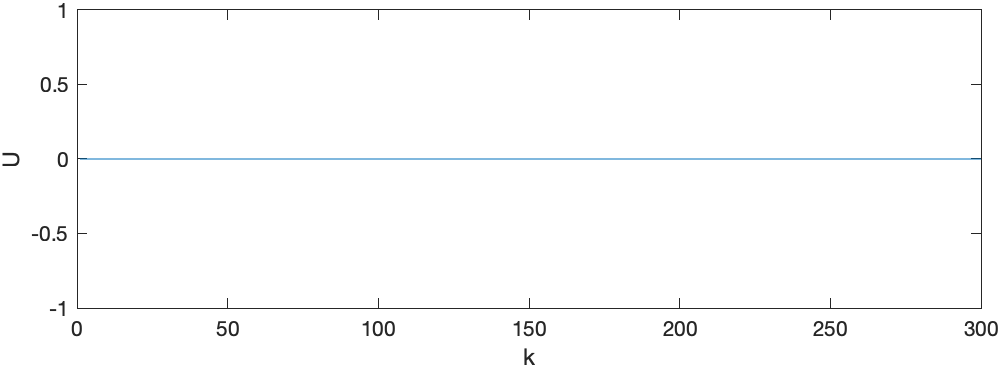
\includegraphics[scale=0.75]{png/projekt/zad1_u.png}
	\caption{Wej�cie uk�adu w punkcie pracy}
	\label{zad1_u}
\end{figure}

\begin{figure}[H]
	\centering
	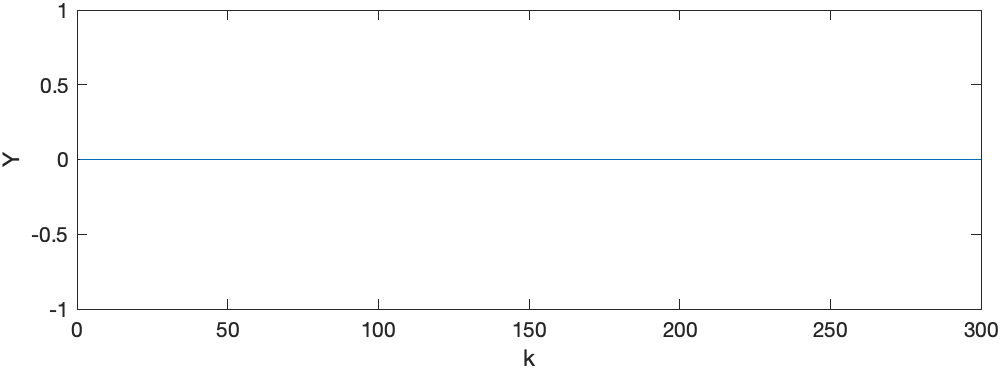
\includegraphics[scale=0.75]{png/projekt/zad1_y.png}
	\caption{Wyj�cie uk�adu w punkcie pracy}
	\label{zad1_y}
\end{figure}

 
\section{Wyznaczenie odpowiedzi skokowych procesu}

Uk�ad zosta� pobudzony sygna�ami o warto�ciach $ U = [-0,8; -0,3; 0,2; 0,6; 1,0]$.

Otrzymane zosta�y w ten spos�b odpowiedzi skokowe:

\begin{figure}[H]
	\centering
	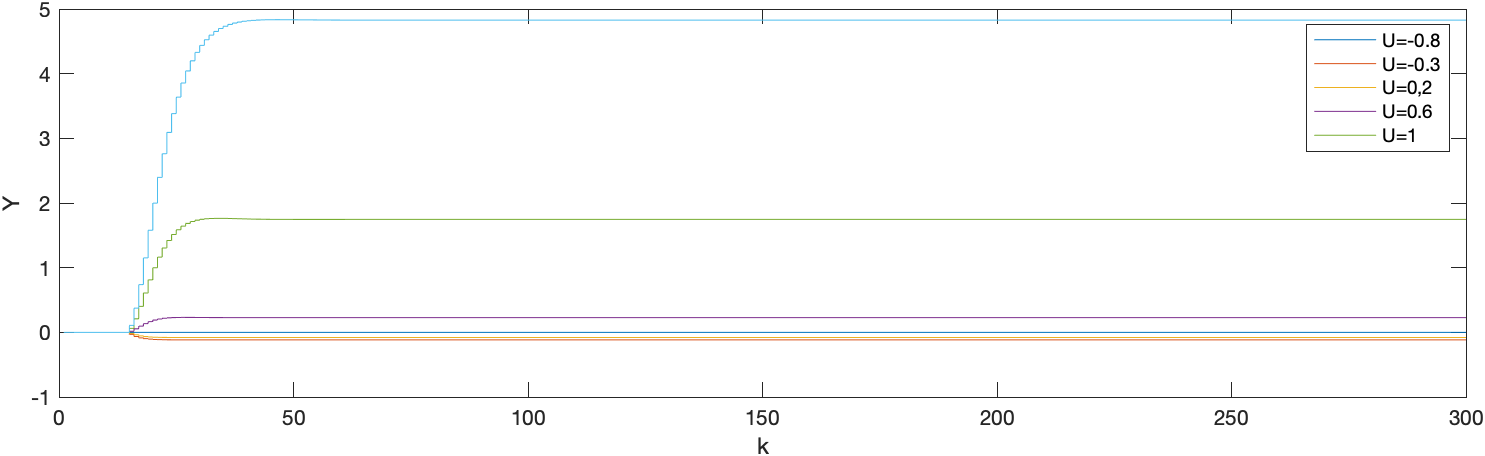
\includegraphics[scale=0.6]{png/projekt/zad2_1.png}
	\caption{Otrzymane odpowiedzi skokowe}
	\label{zad2_1}
\end{figure}

Na wykresie  \ref{zad2_2}  widoczna jest charakterystyka statyczna obiektu.

\begin{figure}[H]
	\centering
	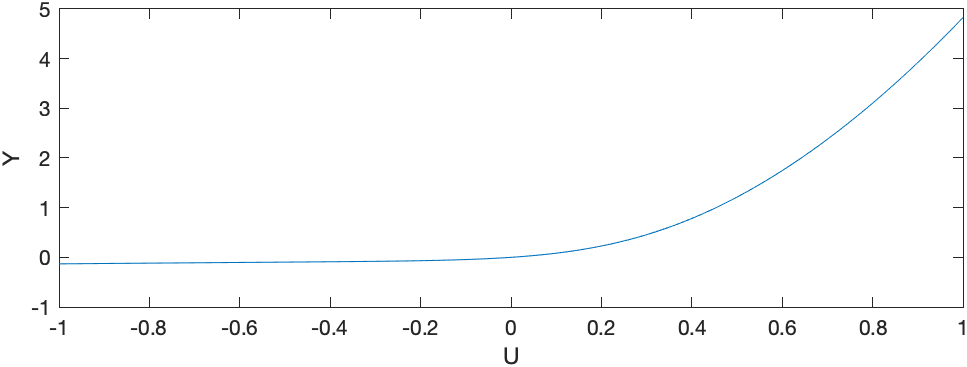
\includegraphics[scale=0.75]{png/projekt/zad2_2.png}
	\caption{Charakterystyka statyczna}
	\label{zad2_2}
\end{figure}

W�a�ciwo�ci dynamiczne oraz statyczne nie s� liniowe. Do charakterystyki statycznej nie mo�e zosta� dopasowana prosta.

\section{Algorytmy PID i DMC}

Obiekt zosta� poddany regulacji za pomoc� algorytm�w PID i DMC z Projektu 2.

TODO opis PID, DMC

\begin{figure}[H]
	\centering
	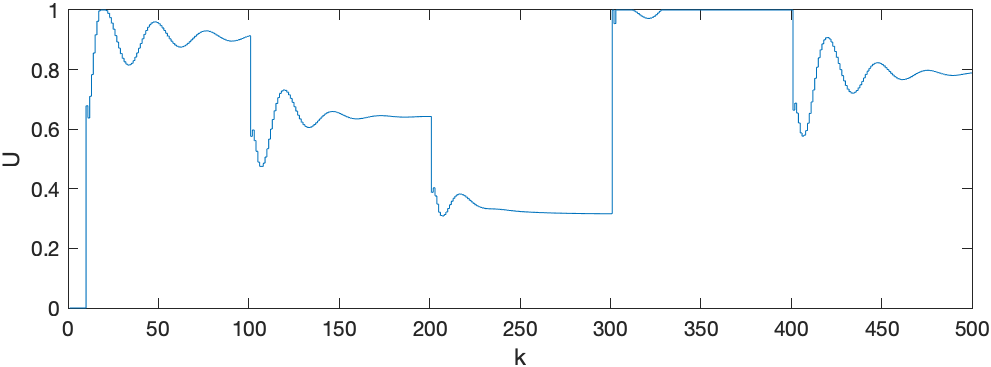
\includegraphics[scale=0.75]{png/projekt/zad3_pid_u.png}
	\caption{Wej�cie uk�adu - algorytm PID}
	\label{zad3_pid_u}
\end{figure}

\begin{figure}[H]
	\centering
	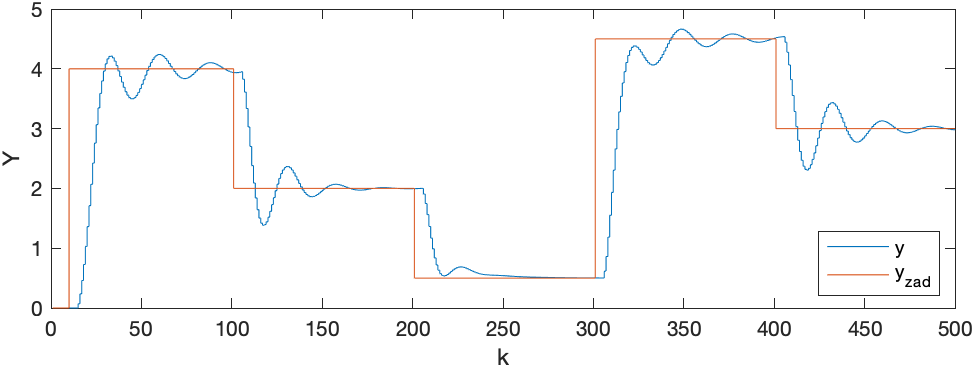
\includegraphics[scale=0.75]{png/projekt/zad3_pid_y.png}
	\caption{Wyj�cie uk�adu - algorytm PID}
	\label{zad3_pid_y}
\end{figure}

\begin{figure}[H]
	\centering
	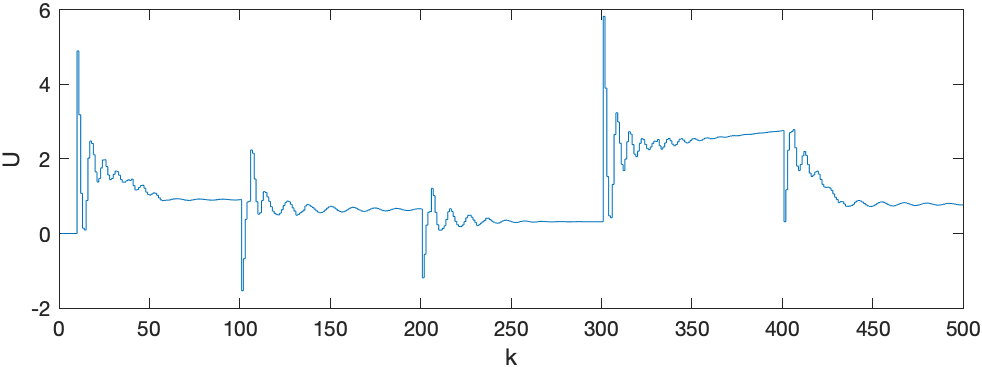
\includegraphics[scale=0.75]{png/projekt/zad3_dmc_u.png}
	\caption{Wej�cie uk�adu - algorytm PID}
	\label{zad3_dmc_u}
\end{figure}

\begin{figure}[H]
	\centering
	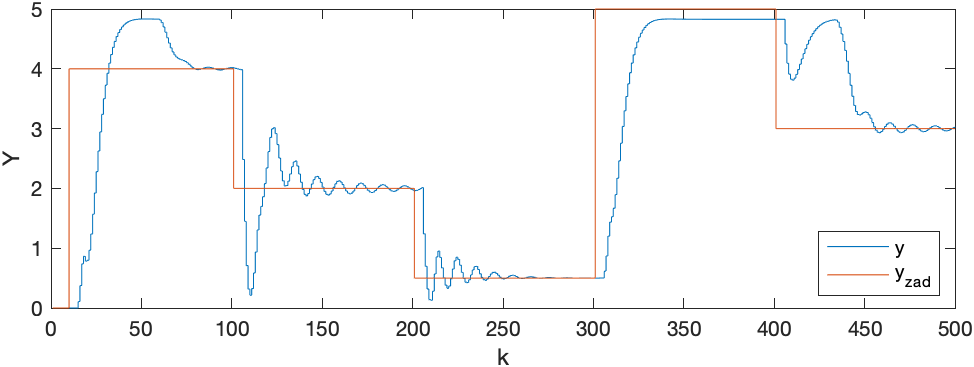
\includegraphics[scale=0.75]{png/projekt/zad3_dmc_y.png}
	\caption{Wyj�cie uk�adu - algorytm PID}
	\label{zad3_dmc_y}
\end{figure}



\section{Rozmyty algorytm PID}

\section{Rozmyty algorytm DMC}


% !TEX encoding = cp1250
\chapter{�wiczenie laboratoryjne}

Podczas tego zadania laboratoryjnego wykorzystano:
\begin{itemize}
	\item grza�k� G1 (sygna� steruj�cy $U$),
	\item wentylator W1 (warto�� zadana $Y_{zad}$),
	\item czujnik temperatury T1 (sygna� wyj�ciowy $Y$) 
\end{itemize} 

\section{Przygotowanie do wykonania �wiczenia}
Przed rozpocz�ciem pomiar�w sprawdzono mo�liwo�� sterowania i~pomiaru w~komunikacji ze stanowiskiem. Punkt pracy grza�ki $G1$ dla zespo�u obliczony zosta� wg. wzoru \ref{w_G1}:
\begin{equation}
	G1 = 25 + Z\%5\
\label{w_G1}
\end{equation}
gdzie Z~to numer zespo�u, zatem dla naszego zespo�u Z02 punkt pracy wynosi:
\begin{equation}
	G1 = 25 + 2\%5 = 27
\end{equation}
Nast�pnie okre�lono warto�� pomiaru temperatury T1 dla obliczonego punktu pracy. W~tym celu moc wentylatora W1 ustawiono na 50\%, a moc grza�ki G1 na 27\%,  za pomoc� funkcji
\texttt{sendControls([1,5], [50,27])}.
Warto�� pomiaru temperatury odczytano korzystaj�c z~funkcji 
\texttt{readMeasurements(1)}.
Temperatura T1 ustabilizowa�a si� na warto�ci \textbf{32.25\degree C}

 
\section{Wyznaczenie odpowiedzi skokowych procesu}
Zarejestrowano przebieg temperatury T1 dla trzech r�nych zmian sygna�u steruj�cego G1 rozpoczynaj�c z~punktu pracy (27\%) do 10\%, 35\% i~50\%.
Otrzymane przebiegi zmian przedstawiono na Rys. \ref{rys_przebiegi_T1}. 

\textcolor{red}{
	Czy w�a�ciwo�ci statyczne obiektu mo�na okre�li� jako (w przybli�eniu) liniowe? Je�li tak wyznaczy� wzmocnienie statyczne procesu?
}

\newpage
\begin{figure}[H]
	\centering
	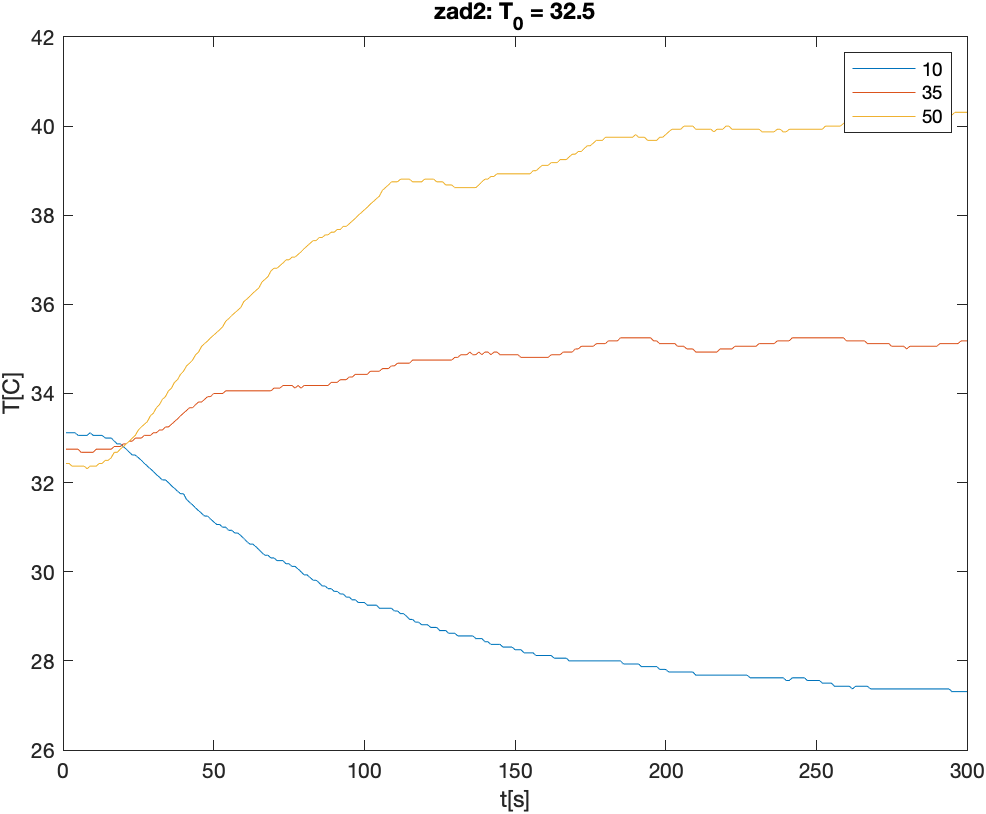
\includegraphics[scale=0.35]{png/lab1_zad2.png}
	\caption{Odpowiedzi skokowe procesu}
	\label{rys_przebiegi_T1}
\end{figure}

\section{Algorytm PID}

Poni�sze zadanie laboratoryjne realizowane by�o w inny, zimniejszy dzie�, co spowodowa�o konieczno�� wyznaczenia warto�ci pomiaru temperatury w punkcie pracy na nowo. Nowy punkt pracy dla ${G1 = 27}$ to ${ T1 = 29.37 }$ {\degree C}.

Napisano  program do regulacji cyfrowego algorytmu PID. Dob�r nastaw regulatora przeprowadzono metod� Zieglera-Nicholsa. Rozpocz�to od doboru warto�ci wzmocnienia K, przy parametrze ca�kuj�cym Ti = inf i r�niczkuj�cym Td = 0. W algorytmie uwzgl�dniono ograniczenia warto�ci sterowania G1(k) (zakres od ${U_{min} = 0}$  do ${\Delta U_{max}=100}$).

Testowano odpowied� uk�adu przy r�nych warto�ciach wzmocnienia K. 
Pocz�tkowo ustawiono zbyt du�� warto�� ${Y_{zad} = 50}$, co uniemo�liwi�o analiz� przebiegu wyj�cia uk�adu � warto�� wzrasta�a powoli, przez co pomiar zajmowa� za du�o czasu. Problem ten widoczny jest na wykresach Rys. {\ref{rys_lab_PID_k18}} i Rys.  {\ref{rys_lab_PID_k20_1}} . Pomiar z Rys. {\ref{rys_lab_PID_k18}} zosta� przerwany po zauwa�eniu nieprzewidywanego zachowania.


\begin{figure}[H]
	\centering
	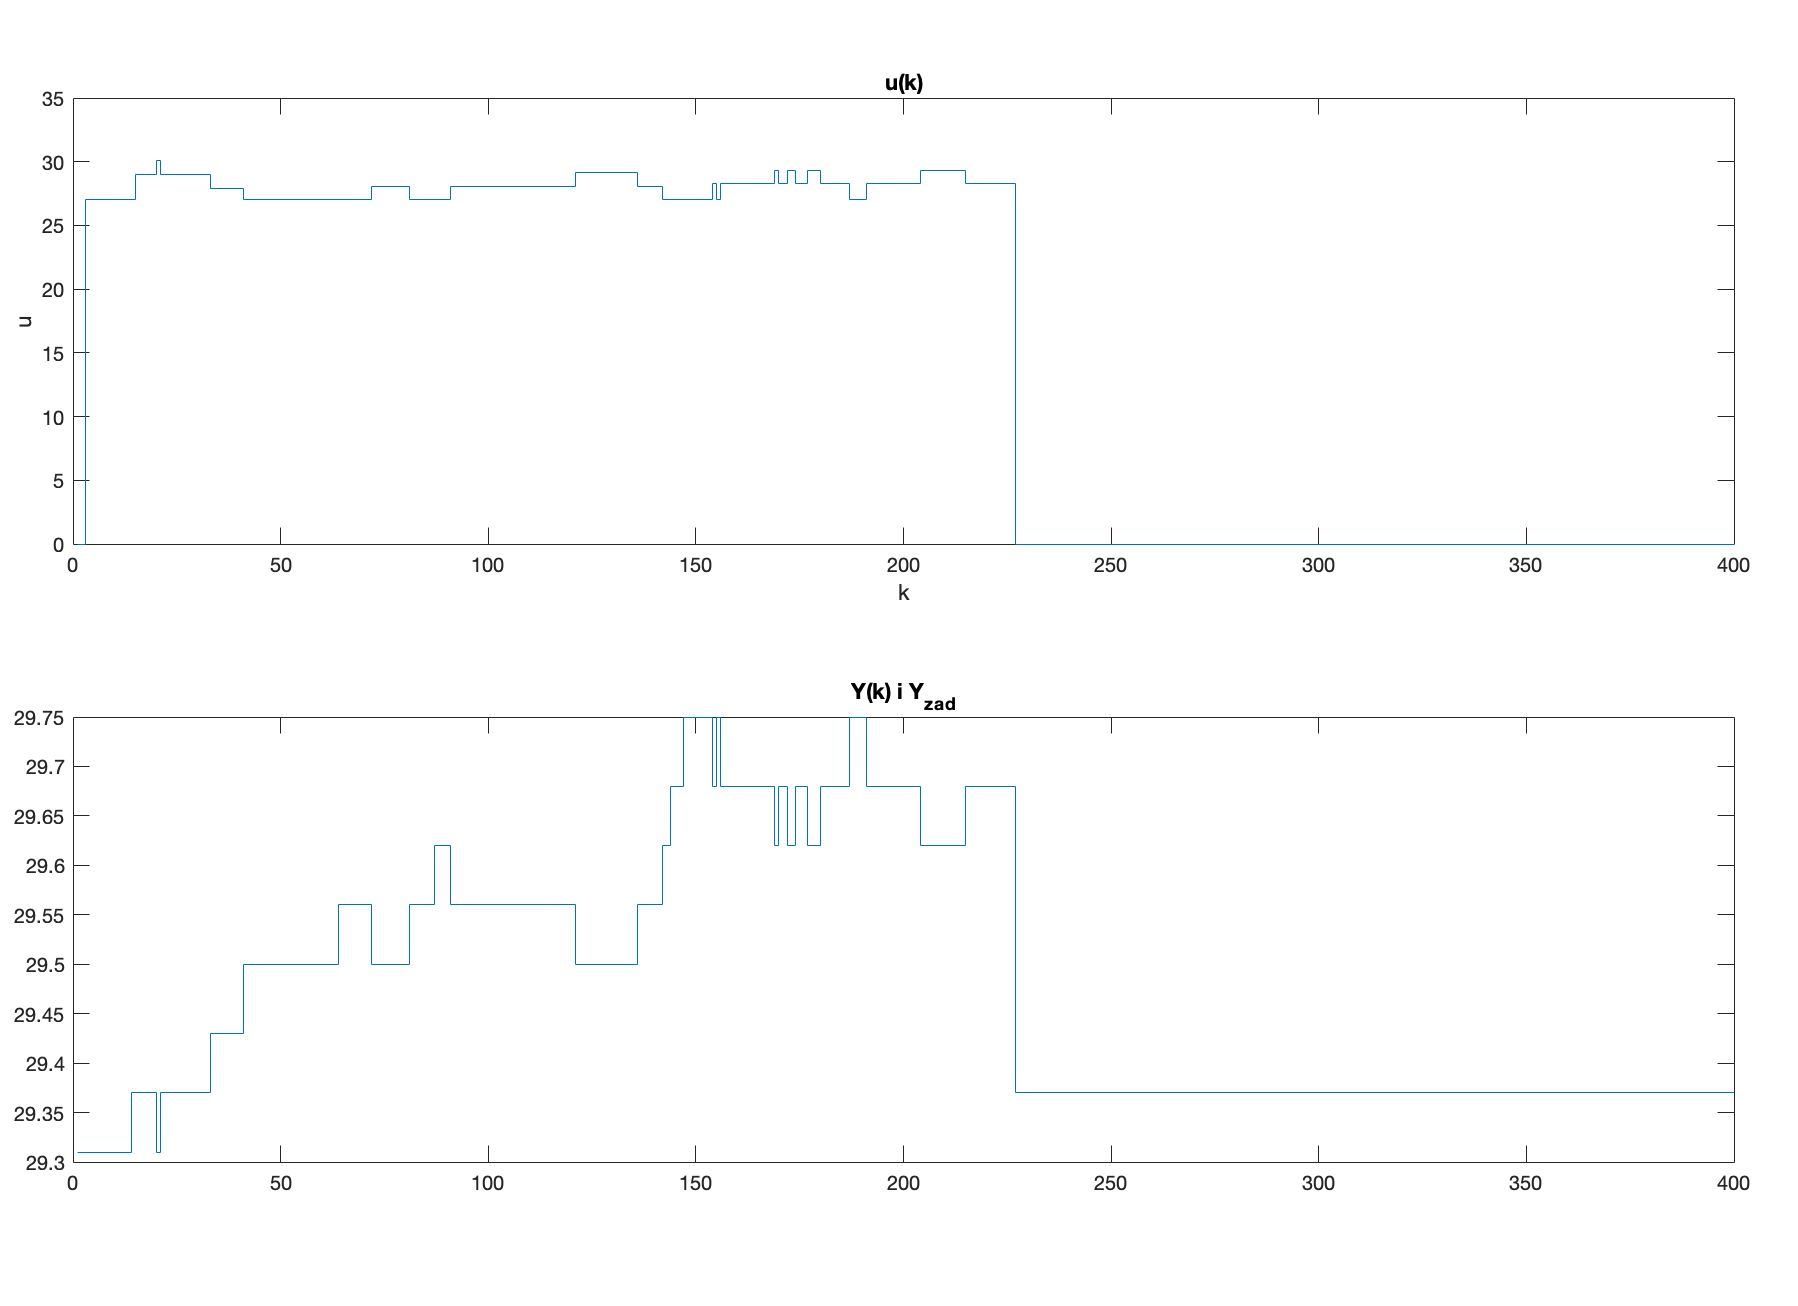
\includegraphics[scale=0.22]{png/lab2/zad5_lab1_pid_k18.png}
	\caption{Przebiegi dla ${K = 18}$ i ${Y_{zad} = 50}$}
	\label{rys_lab_PID_k18}
\end{figure}


\begin{figure}[H]
	\centering
	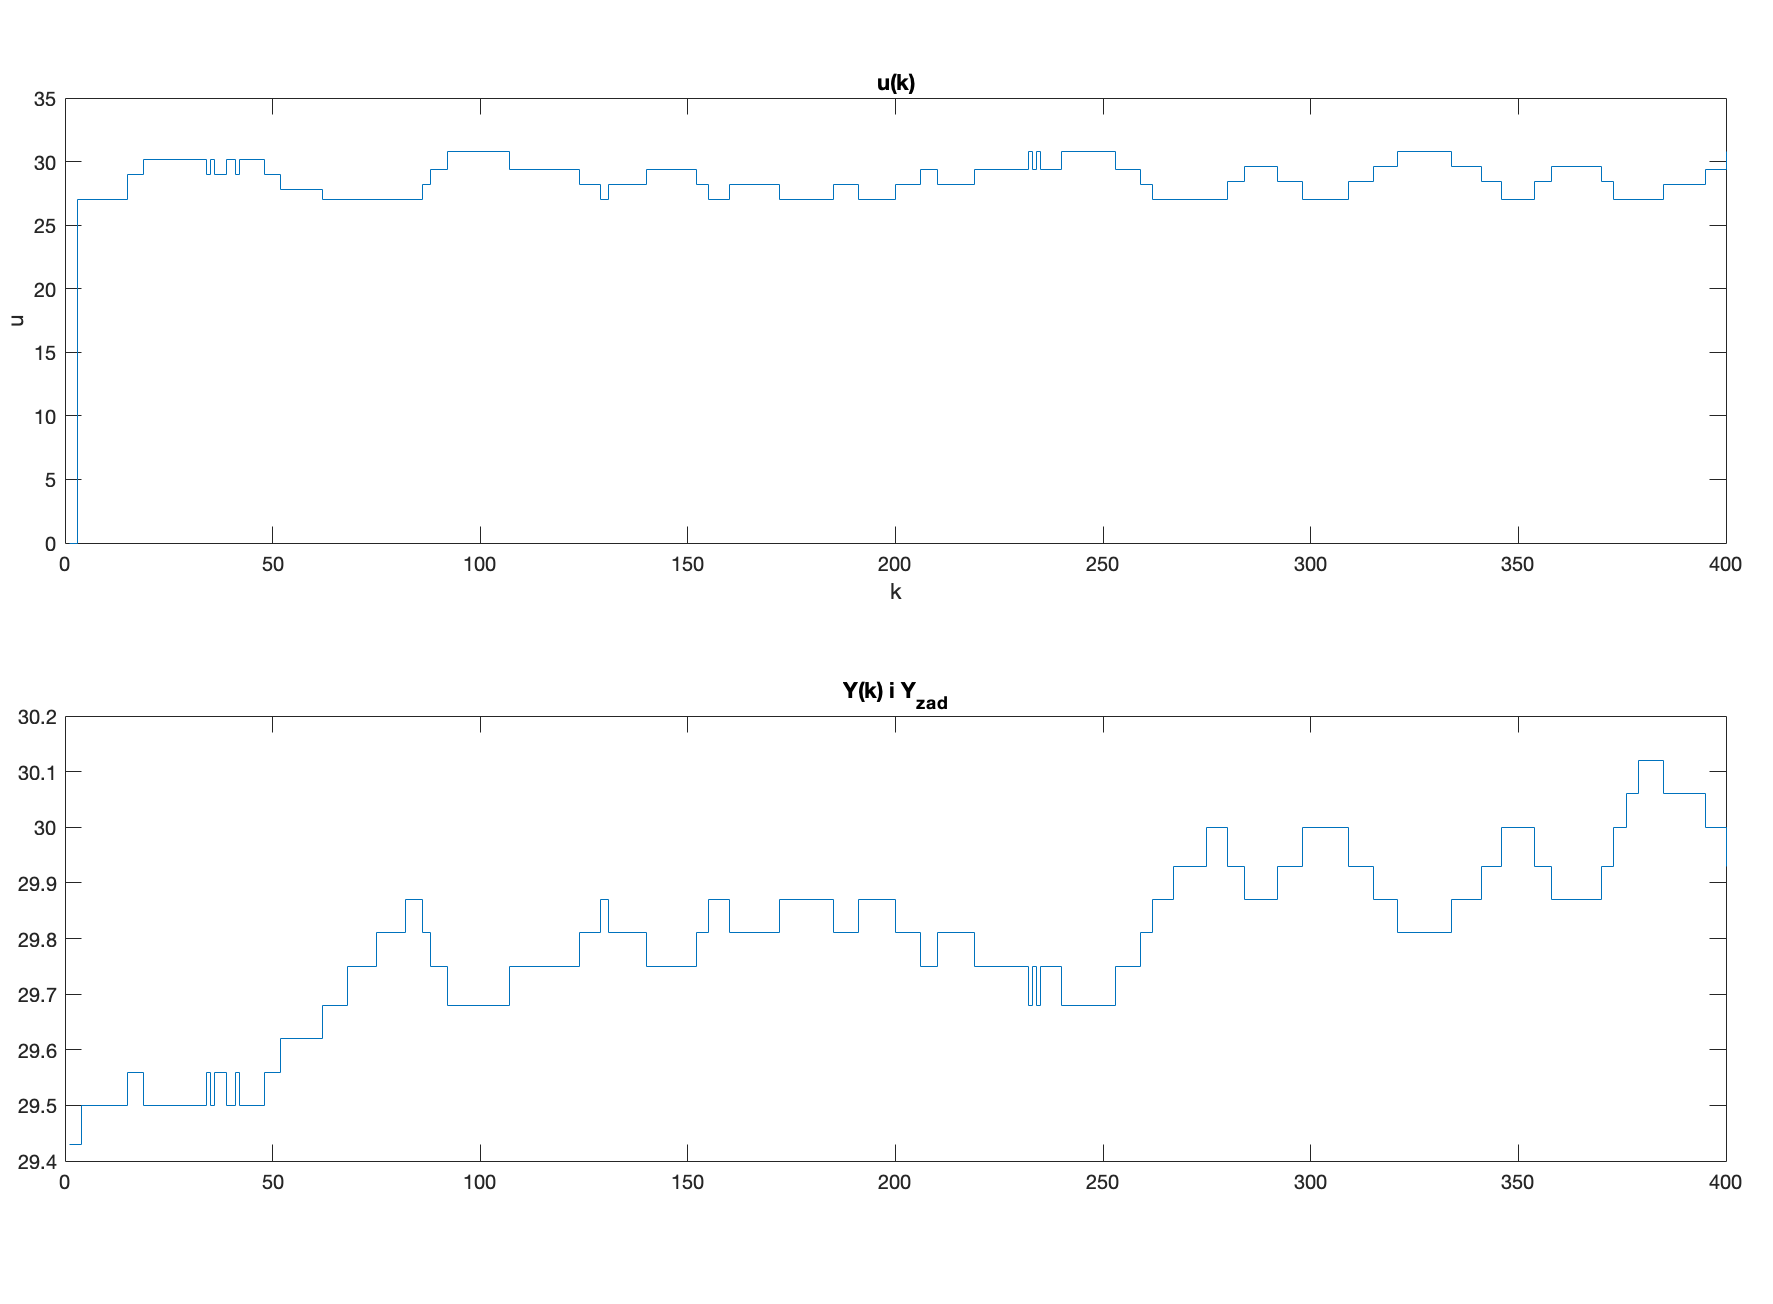
\includegraphics[scale=0.22]{png/lab2/zad5_lab1_pid_k20_v1.png}
	\caption{Przebiegi dla ${K = 20}$ i ${Y_{zad} = 50}$}
	\label{rys_lab_PID_k20_1}
\end{figure}


Po zaobserwowaniu powy�szego problemu i jego analizie zmieniono warto�� sygna�u zadanego na ${Y_{zad} = 33}$. Wyniki widoczne s� na wykresie Rys.  {\ref{rys_lab_PID_k20_2}}.


\begin{figure}[H]
	\centering
	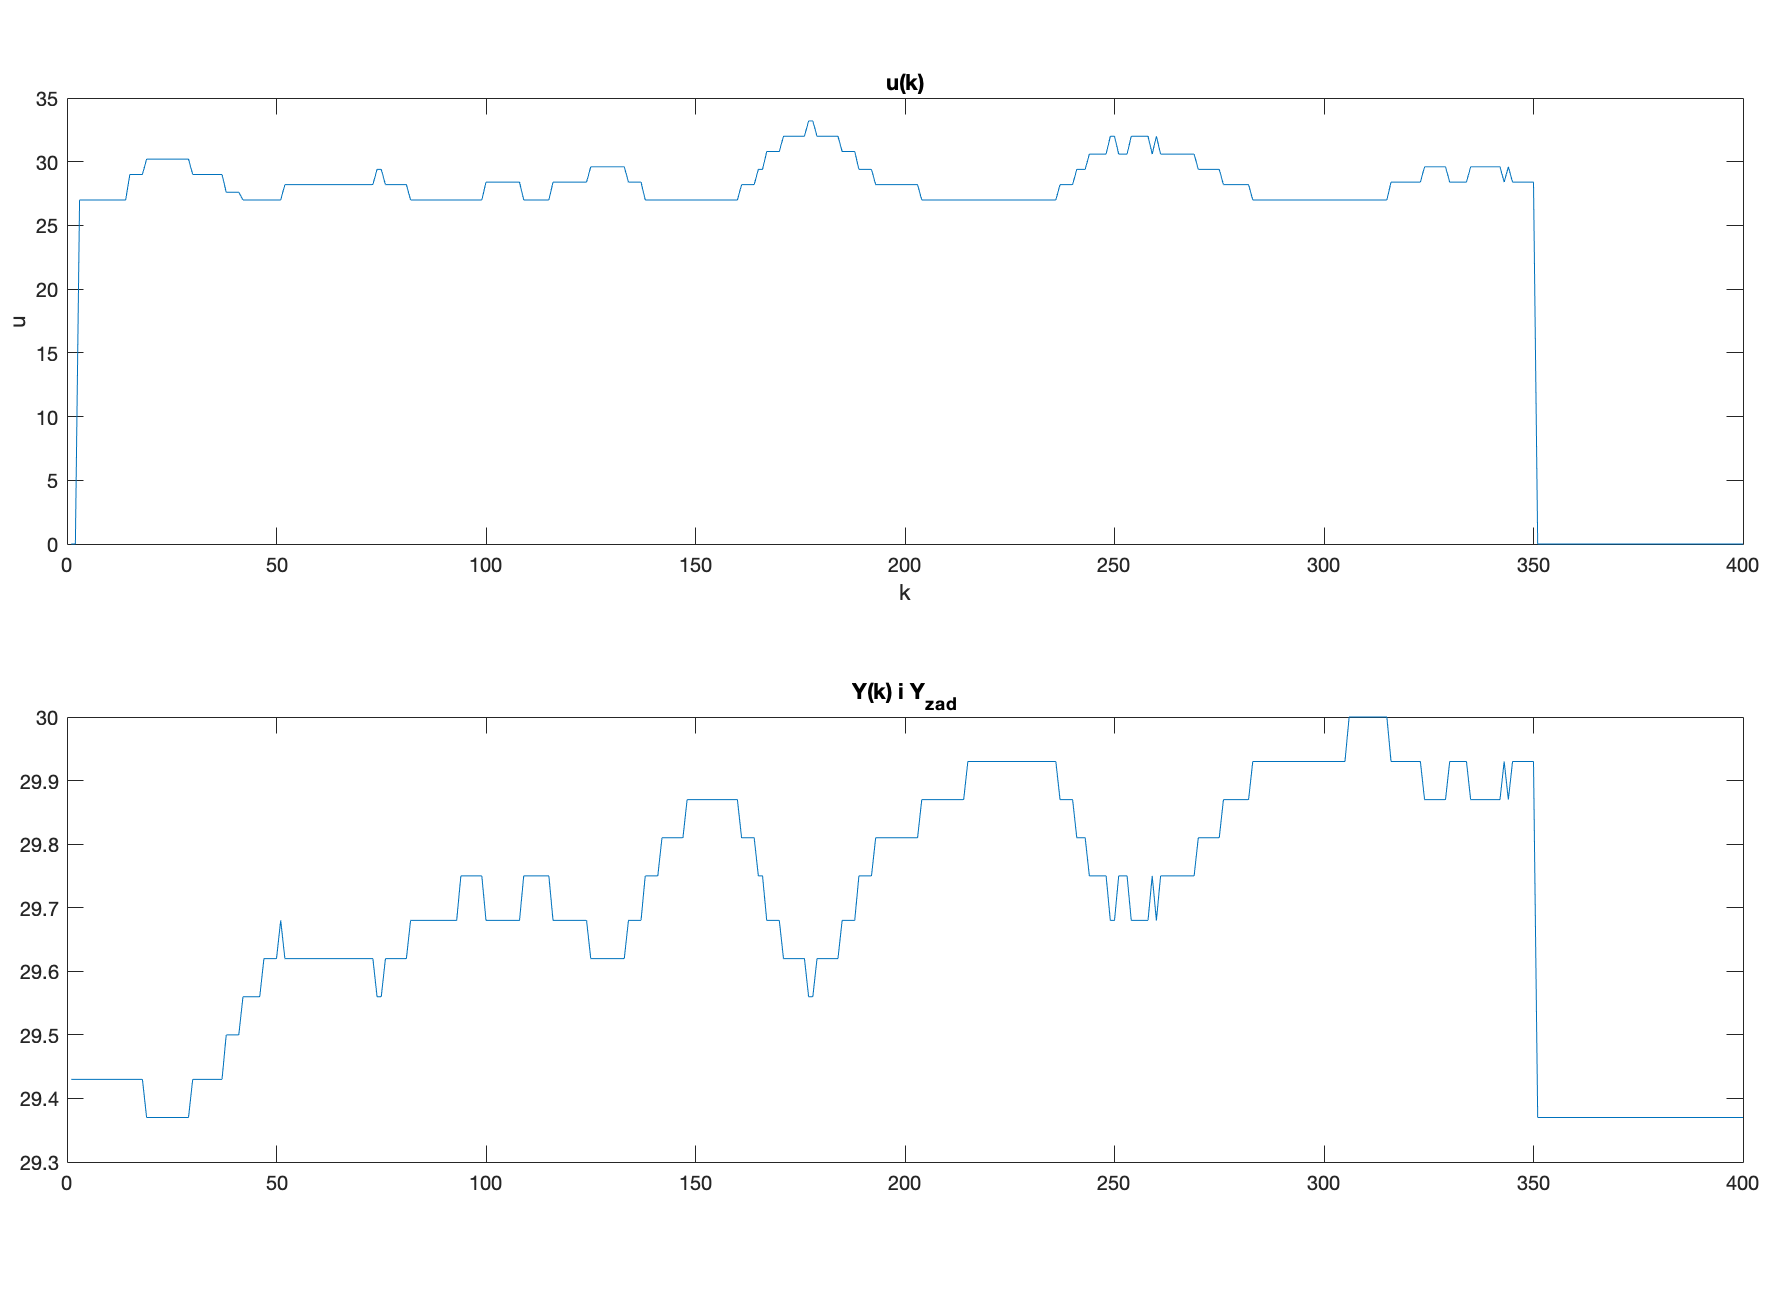
\includegraphics[scale=0.22]{png/lab2/zad5_lab1_pid_k20_v2.png}
	\caption{Przebiegi dla ${K = 20}$ i ${Y_{zad} = 33}$}
	\label{rys_lab_PID_k20_2}
\end{figure}

Mimo tej zmiany, odpowied� procesu nadal ros�a zbyt wolno. Po ponownej analizie algorytmu wywnioskowano, �e do niskiej pr�dko�ci wzrastania przyczyni� si� r�wnie� niew�a�ciwie dobrany parametr ${\Delta U_{max}=2}$ � ogranicza� on bowiem szybko�� zmian sygna�u steruj�cego. Po zmianie tej warto�ci na ${\Delta U_{max} = 20}$, uk�ad dzia�a� zgodnie z za�o�eniami (Rys. {\ref{rys_lab_PID_k20_3}}). 


\begin{figure}[H]
	\centering
	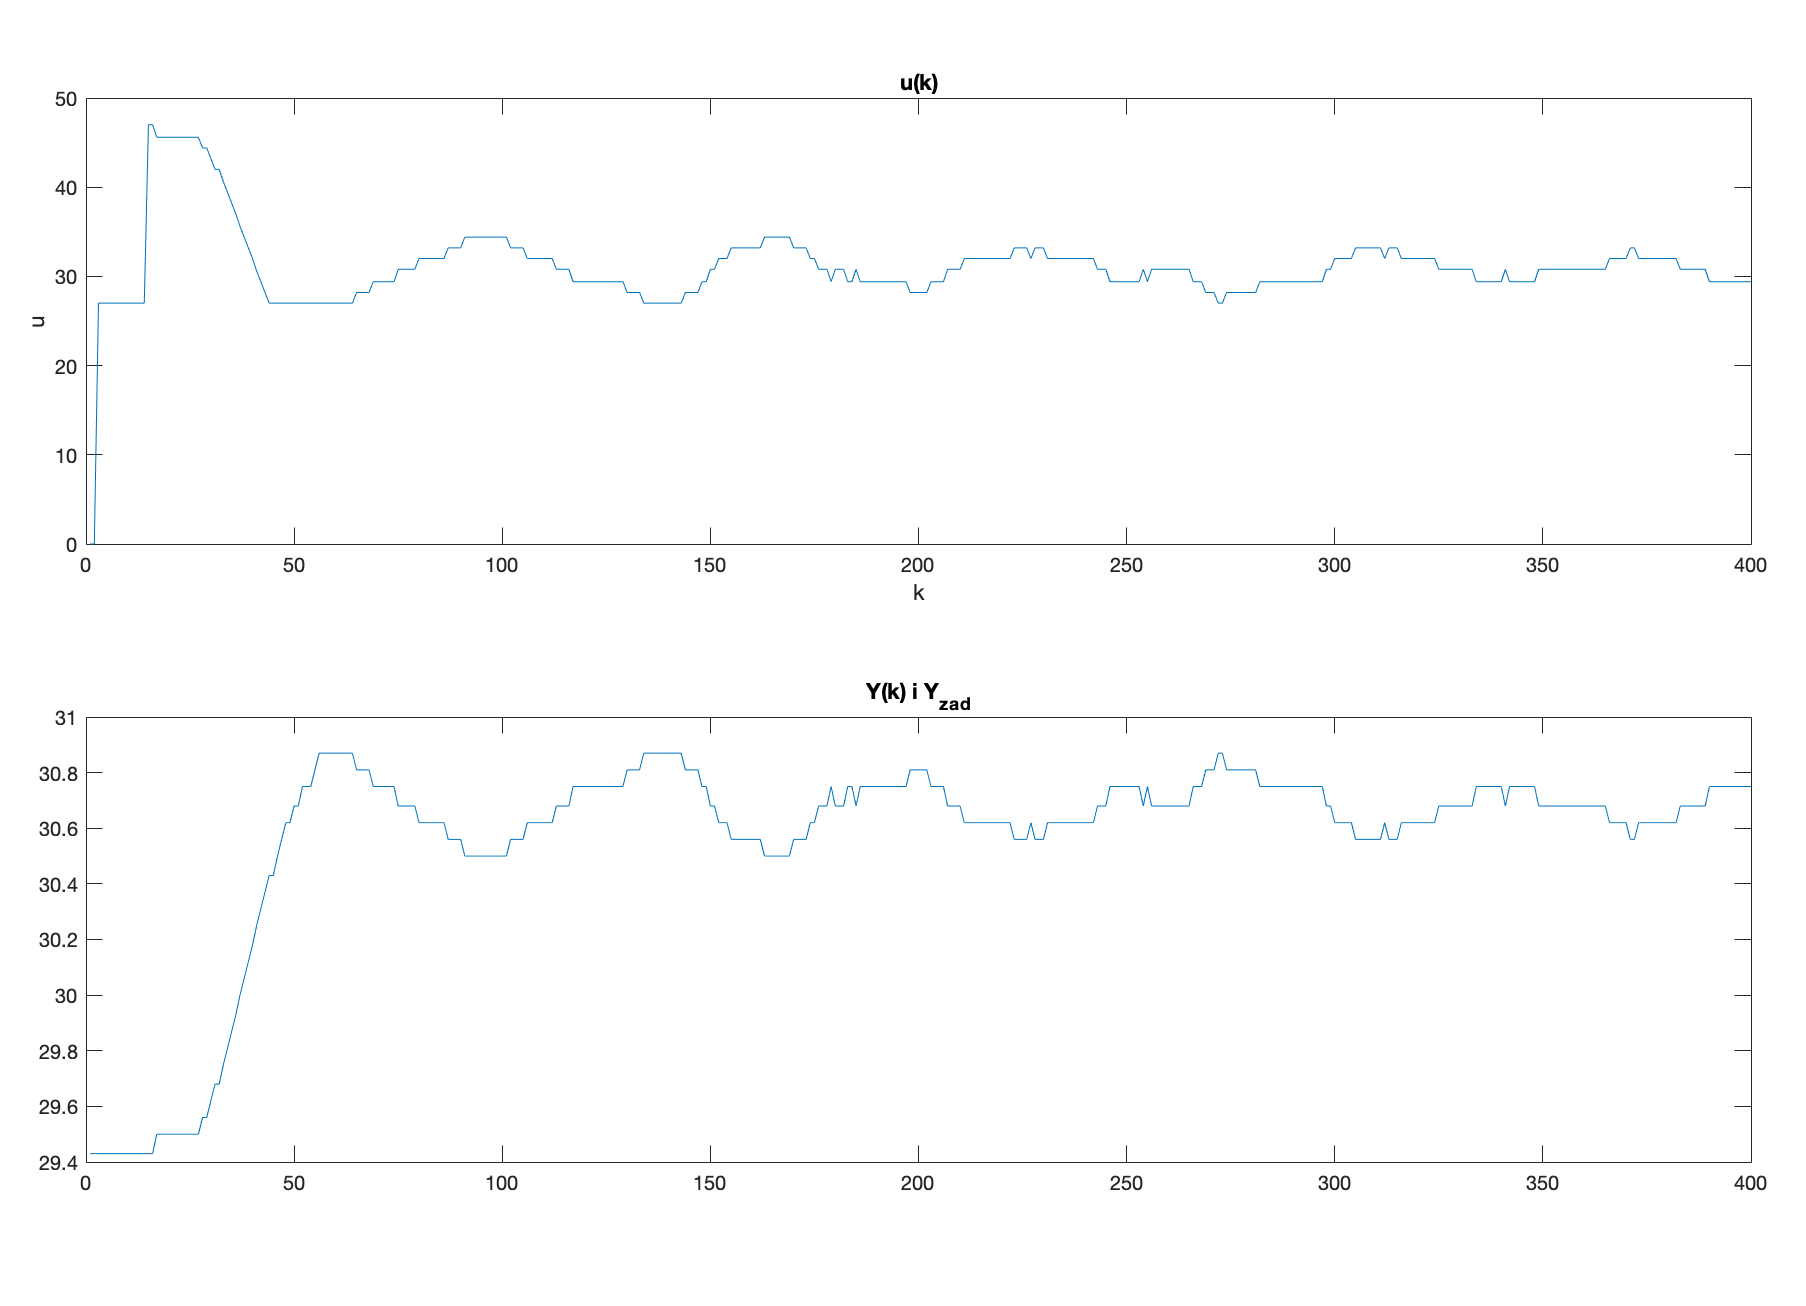
\includegraphics[scale=0.22]{png/lab2/zad5_lab1_pid_k20_v3.png}
	\caption{Przebiegi dla ${K = 20}$, ${Y_{zad} = 33}$ i zmienion� warto�ci� ${\Delta U_{max}}$}
	\label{rys_lab_PID_k20_3}
\end{figure}

Widoczne s� regularne oscylacje, jednak s� one oscylacjami gasn�cymi. Warto�� wzmocnienia zosta�a wi�c zwi�kszona do ${K = 24}$. Jak wida� na wykresie Rys. {\ref{rys_lab_PID_k24}} oscylacje nie gasn�. Zauwa�alny jest  nawet lekki wzrost amplitudy oscylacji. Przewidujemy, �e niegasn�ce oscylacje wyst�pi�yby przy warto�ci wzmocnienia ${K_{kr}=23}$, jednak przez problemy wyst�puj�ce na pocz�tku realizacji zadania nie zosta�o to sprawdzone.
Z tego powodu nie dobrano r�wnie� pozosta�ych parametr�w regulatora PID dla zmiennego sygna�u zadanego. 
Je�li zesp� mia�by wi�cej czasu, nast�pnym krokiem by�oby ustawienie nastaw regulatora wg. regu� Zieglera-Nicholsa (Rys. {\ref{t_ZN}}). Zatem po wyznaczeniu wzmocnienia krytycznego ${K_{kr}}$, z przebiegu warto�ci sterowania odczytany zosta�by okres krytyczny ${T_{kr}}$, a wst�pne nastawy regulatora PID wynosi�yby: ${K=0.6K_{kr}}$, ${T_i= 0.5T_{kr}}$ i ${T_d=0.125K_{kr}}$. Je�eli by�oby to konieczne, regulator zosta�by dostrojony metod� eksperymentaln�.


\begin{figure}[H]
	\centering
	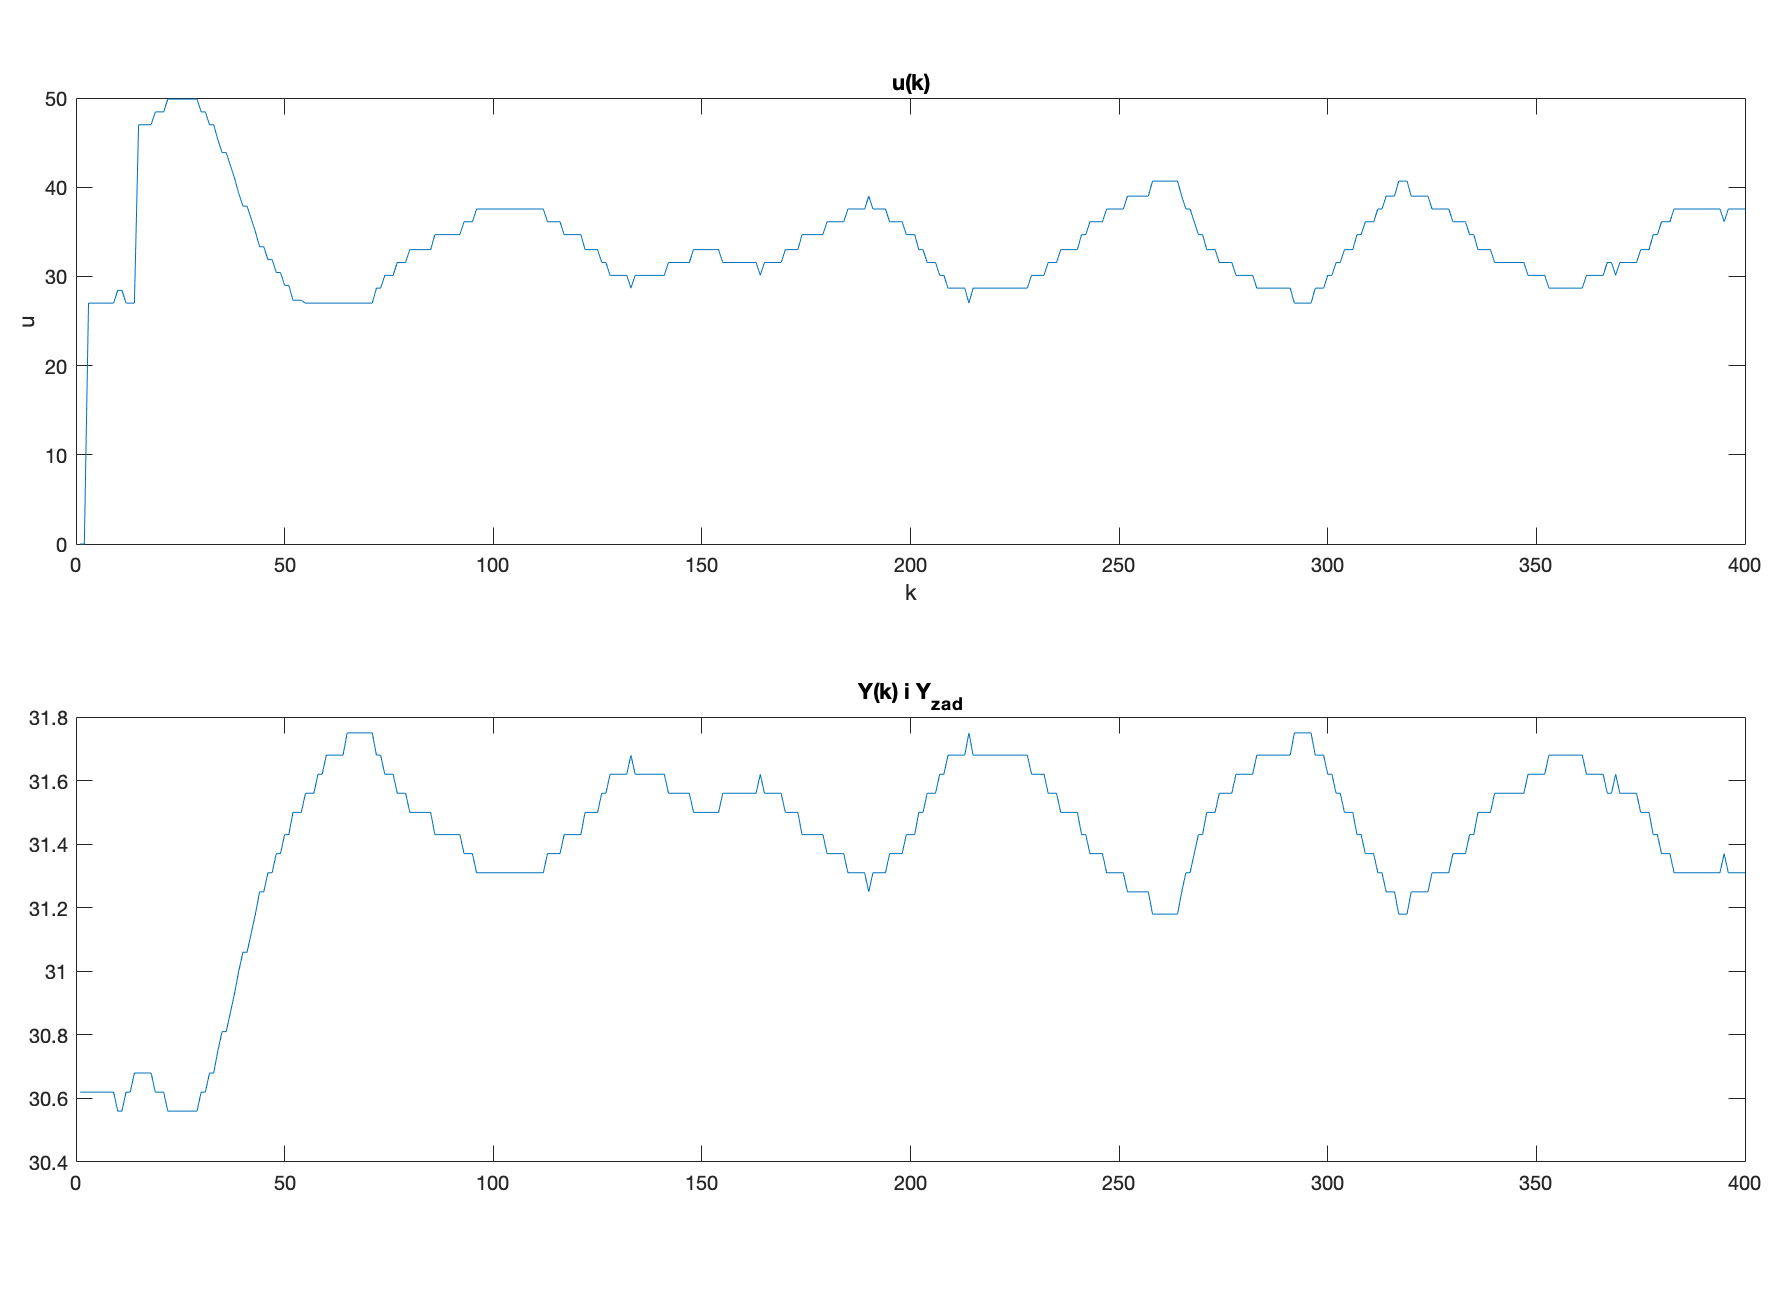
\includegraphics[scale=0.22]{png/lab2/zad5_lab1_pid_k24.png}
	\caption{Przebiegi dla ${K=24}$}
	\label{rys_lab_PID_k24}
\end{figure}



\section{Algorytm DMC}




%% !TEX encoding = cp1250
\chapter{Wzory matematyczne}
Stosujemy przecinek dziesi?tny, a~nie kropk? dziesi?tn?. Aby unikn?? dodatkowego odst?pu, stosujemy zapis \verb+\num{1,2345}+ lub \verb+\num{1.2345}+, co prowadzi do \num{1,2345}, a~nie \verb+$1,2345$+, co prowadzi do $1,2345$. Stosujemy zapis \num{1.2345e10}, a~nie $1{,}2345\times 10^{10}$. Powy?szy zapis mo?na stosowa? r�wnie? w trybie matematycznym, np. \verb+$\num{1.2345e10}$+ skompiluje si? do $\num{1.2345e10}$.

\section{Sta?e i~zmienne, indeksowanie}
Skalarne sta?e i~zmienne zapisujemy w~trybie matematycznym, np. $x$, $y$, $z$. Stosujemy indeksy dolne, np. $x_i$, g�rne, np. $x^j$, lub oba, np. $x_i^j$. Mo?na r�wnie? zastosowa? indeksy w~nawiasach, np. $y(k)$. Je?eli indeks zapisany jest czcionk? pochy??, spodziewamy si?, ?e przyjmuje on warto?? liczbow? (liczby naturalne), np. $x_i$ dla $i=1,\ldots,10$. Je?eli natomiast zastosujemy oznaczenie $x_{\mathrm{i}}$, to w�wczas indeks $\mathrm{i}$ nie przyjmuje ?adnej warto?ci, jest on integraln? cz??ci? zmiennej lub sta?ej. Dlatego oznaczaj?c horyzont sterowania stosujemy symbol $N_{\mathrm{u}}$, a~nie $N_u$, co by sugerowa?o, ?e indeks $u$ przyjmuje pewne warto?ci z zakresu liczb naturalnych. Analogicznie, sta?a czasowa ca?kowania oznaczana jest jako $T_{\mathrm{i}}$, a~nie jako $T_i$, sta?a czasowa r�?niczkowania to $T_{\mathrm{d}}$, a nie $T_d$. Sygna? warto?ci zadanej oznaczamy przez $y^{\mathrm{zad}}$, a~nie przez $y^{zad}$.

Nie nale?y stosowa? czcionki pochy?ej r�wnie? do tekst�w, kt�re uzupe?niaj? wyra?enia matematyczne, np. zamiast b??dnej postaci
\begin{equation}
y(x)=
\begin{cases}
x^2 & gdy \ x\le 0\\
x^3 & gdy \ x>0
\end{cases}
\nonumber
\end{equation}
powinno by?
\begin{equation}
y(x)=
\begin{cases}
x^2 & \textrm{gdy } x\le 0\\
x^3 & \textrm{gdy } x>0
\end{cases}
\nonumber
\end{equation}
Odst?py w trybie matematycznym wymuszamy za pomoc? instrukcji \verb+\+, \verb+\quad+, \verb+\qquad+ itd.

\section{Wektory}
Do oznaczenia wektor�w najcz??ciej stosujemy symbole pogrubione, np. $\boldsymbol{x}$, $\triangle\boldsymbol{u}(k)$. Pami?tamy, ?e w matematyce wektory zawsze s? pionowe. Wektory, kt�rych elementami s? skalary, zapisujemy wi?c jako
\begin{equation}
\triangle\boldsymbol{u}(k)=\left[\triangle u(k|k) \ \ldots \ \triangle u(k+N_{\mathrm{u}}-1|k) \right]^{\mathrm{T}}
\end{equation}
lub w~postaci
\begin{equation}
\triangle\boldsymbol{u}(k)=\left[
\begin{array}{c}
\triangle u(k|k)\\
\vdots\\
\triangle u(k+N_{\mathrm{u}}-1|k)
\end{array}
\right]
\label{w_dUk}
\end{equation}
Je?eli u?ywamy wektor�w, kt�rych elementami sk?adowymi s? inne wektory, najwygodniej zapisa? je pionowo. Np. elementami wektora (\ref{w_dUk}) s? podwektory
\begin{equation}
\triangle u(k+p|k)=\left[
\begin{array}{c}
\triangle u_1(k+p|k)\\
\vdots\\
\triangle u_{n_{\mathrm{u}}}(k+p|k)
\end{array}
\right]
\label{w_dukp}
\end{equation}
gdzie $p=1,\ldots,N_{\mathrm{u}}$. A wi?c ka?dy z~wektor�w (\ref{w_dukp}) ma d?ugo?? $n_{\mathrm{u}}$, wektor (\ref{w_dUk}) ma d?ugo?? $n_{\mathrm{u}}N_{\mathrm{u}}$.

\section{Macierze}
Do oznaczenia macierzy najcz??ciej stosujemy symbole pogrubione, np. macierz dynamiczna w~algorytmie DMC dla procesu o~jednym wej?ciu i~jednym wyj?ciu ma wymiar $N \times N_{\mathrm{u}}$ i struktur?
\begin{equation}
\boldsymbol{G}=\left[
\begin{array}
{cccc}
s_{1} & 0 & \ldots & 0\\
s_{2} & s_{1} & \ldots & 0\\
\vdots & \vdots & \ddots & \vdots\\
s_{N} & s_{N-1} & \ldots &  s_{N-N_{\mathrm{u}}+1}
\end{array}
\right]
\end{equation}
W~przypadku procesu o~$n_{\mathrm{u}}$ wej?ciach i~$n_{\mathrm{y}}$ wyj?ciach ma ona  wymiar $N\times N_{\mathrm{u}}$ i posta?
\begin{equation}
\boldsymbol{G}=\left[
\begin{array}
{cccc}
\boldsymbol{S}_{1} & \boldsymbol{0}_{n_{\mathrm{y}}\times n_{\mathrm{u}}} & \ldots & \boldsymbol{0}_{n_{\mathrm{y}}\times n_{\mathrm{u}}}\\
\boldsymbol{S}_{2} & \boldsymbol{S}_{1} & \ldots & \boldsymbol{0}_{n_{\mathrm{y}}\times n_{\mathrm{u}}}\\
\vdots & \vdots & \ddots & \vdots\\
\boldsymbol{S}_{N} & \boldsymbol{S}_{N-1} & \ldots &  \boldsymbol{S}_{N-N_{\mathrm{u}}+1}%
\end{array}
\right]
\label{w_G}
\end{equation}
gdzie ka?da z~macierzy sk?adowych ma wymiar $n_{\mathrm{y}}\times n_{\mathrm{u}}$
\begin{equation}
\boldsymbol{S}_p=\left[
\begin{array}
{ccc}
s_p^{1,1} & \ldots & s_p^{1,n_{\mathrm{u}}}\\
\vdots & \ddots & \vdots\\
s_p^{n_{\mathrm{y}},1} & \ldots & s_p^{n_{\mathrm{y}},n_{\mathrm{u}}}
\end{array}
\right]
\end{equation}
gdzie $p=1,\ldots,N$. A~wi?c macierz (\ref{w_G}) ma wymiar $n_{\mathrm{y}}N\times n_{\mathrm{u}}N_{\mathrm{u}}$.

\section{Wi?ksze wyra?enia matematyczne}
W~przypadku d?ugich wzor�w nie nale?y korzysta? z~otoczenia \verb+equation+, poniewa? wz�r taki zwykle nie~mie?ci si? na stronie o przyj?tej szeroko?ci, np.
\begin{equation}
y(k)=b_1u(k-1)+b_2u(k-2)+b_3u(k-3)+b_4u(k-4)+b_5u(k-5)-a_1y(k-1)-a_2y(k-2)-a_3y(k-3)-a_4y(k-4)-a_5y(k-5)
\end{equation}
Nale?y zastosowa? otoczenie \verb+align+, co prowadzi do wzoru
\begin{align}
y(k)&=b_1u(k-1)+b_2u(k-2)+b_3u(k-3)+b_4u(k-4)+b_5u(k-5)\nonumber\\
&\quad -a_1y(k-1)-a_2y(k-2)-a_3y(k-3)-a_4y(k-4)-a_5y(k-5)\label{w_yk}
\end{align}
Nie stosujemy otoczenia \verb+split+ z~powodu b??dnego centrowania. Numer wzoru z?o?onego z~wielu wierszy umieszczamy tylko w~ostatnim wierszu.





%\chapter{Tabele}
W~praktyce bardzo cz�sto nale�y wyr�wna� liczby wzgl�dem cyfr znacz�cych w~poszczeg�lnych kolumnach (czyli przecinek dziesi�tny ma by� we wszystkich wierszach tabeli umieszczony w~tym samym miejscu w~pionie). Do wyr�wnania liczb nale�y wykorzysta� pakiet \verb+siunitx+ (pakiety \verb+rccol+ oraz \verb+dcolumn+ maj� mniejsze mo�liwo�ci). Wszystkie przyk�ady podane w~niniejszym rozdziale wykorzystuj� pakiet \verb+siunitx+. Zwr��my uwag�, �e tytu�y znajduj�ce si� w~pierwszym wierszu wszystkich tabel s� wy�rodkowane (w~obr�bie kolejnych kom�rek).

Je�eli standardowa szeroko�� kolumn jest za ma�a, nale�y w~dowolnym wierszu wstawi� z~obu stron zawarto�ci kom�rki polecenia \verb+\hspace{odleg�o��}+, kt�re zapewniaj� odpowiedni� szeroko��. Modyfikacj� tak� zastosowano w~drugiej kolumnie tab.~\ref{t_wyrownanie_do_znaku_przecinek3}.

Je�eli tabela jest szersza ni� szeroko�� strony, nale�y zastosowa� otoczenie \verb+sidewaystable+ z~pakietu \verb+rotating+, co wykorzystano w~tab.~\ref{t_wyrownanie_do_znaku_przecinek4}.

W~zamieszczonych tabelkach wykorzystano polecenie \verb+\rule+ do wstawienia linii o~zerowej szeroko�ci do wierszy tabelek, kt�re s� zbyt w�skie.

\begin{table}
	[b] \caption{Por�wnanie liczby parametr�w~(LP) i~dok�adno�ci~(SSE) modeli}
	\label{t_wyrownanie_do_znaku_przecinek1}
	\centering
	\sisetup{table-format = 2.4}
	\begin{small}
		\begin{tabular}{|l|S[table-format=2]|S|S|S|}
			\hline
			\multicolumn{1}{|c|}{Model\rule{0pt}{3.5mm}} & LP & $\mathrm{SSE_{ucz}}$ & $\mathrm{SSE_{wer}}$ & $\mathrm{SSE_{test}}$ \\ \hline
			Liniowy \rule{0pt}{3.5mm}                    &  4 & 90.1815              & 70.7787              & \textemdash         \\
			Neuronowy, $K=1$                             &  7 & 10.1649              & 10.3895              & \textemdash         \\
			Neuronowy, $K=2$                             & 13 & 0.3282               & 0.3257               & \textemdash         \\
			Neuronowy, $K=3$                             & 19 & 0.2014               & 0.1827               & 0.1468                \\
			Neuronowy, $K=4$                             & 25 & 0.1987               & 0.1906               & \textemdash         \\
			Neuronowy, $K=5$                             & 31 & 0.1364               & 0.1971               & \textemdash         \\
			Neuronowy, $K=6$                             & 37 & 0.1340               & 0.2044               & \textemdash         \\ \hline
		\end{tabular}
	\end{small}
\end{table}

\begin{table}
	[b] \caption{Por�wnanie liczby parametr�w~(LP) i~dok�adno�ci~(SSE) modeli}
	\label{t_wyrownanie_do_znaku_przecinek2}
	\centering
	\sisetup{table-format = 1.4e-1}
	\begin{small}
		\begin{tabular}{|l|S[table-format=2]|S|S|S|}
			\hline
			\multicolumn{1}{|c|}{Model\rule{0pt}{3.5mm}} & LP & $\mathrm{SSE_{ucz}}$ & $\mathrm{SSE_{wer}}$ & $\mathrm{SSE_{test}}$ \\ \hline
			Liniowy\rule{0pt}{3.5mm} &  4 & 9.1815e1  & 7.7787e1  & \textemdash\\
			Neuronowy, $K=1$         &  7 & 1.1649e1  & 1.3895e1  & \textemdash\\
			Neuronowy, $K=2$         & 13 & 3.2821e-1 & 3.2568e-1 & \textemdash\\
			Neuronowy, $K=3$         & 19 & 2.0137e-1 & 1.8273e-1 & 1.4682e-1\\
			Neuronowy, $K=4$         & 25 & 1.9868e-1 & 1.9063e-1 & \textemdash\\
			Neuronowy, $K=5$         & 31 & 1.3642e-1 & 1.9712e-1 & \textemdash\\
			Neuronowy, $K=6$         & 37 & 1.3404e-1 & 2.0440e-1 & \textemdash\\ \hline
		\end{tabular}
	\end{small}
\end{table}

\begin{table}
	[b] \caption{Por�wnanie z�o�ono�ci obliczeniowej}
	\label{t_wyrownanie_do_znaku_przecinek3}
	\centering
	\sisetup{table-auto-round=true}
	\begin{small}
		\begin{tabular}{|l|S[table-format=2]|S[table-format=1.2]|S[table-format=1.2]|S[table-format=2.2]|S[table-format=2.2]|S[table-format=2.2]|S[table-format=3.2]|}
			\hline
			\multicolumn{1}{|c|}{Algorytm\rule{0pt}{3.25mm}} & \hspace{0.5cm} $N$ \hspace{0.5cm} & ${N_{\mathrm{u}}=1}$ & ${N_{\mathrm{u}}=2}$ & ${N_{\mathrm{u}}=3}$ & ${N_{\mathrm{u}}=4}$ & ${N_{\mathrm{u}}=5}$ & ${N_{\mathrm{u}}=10}$ \\ \hline
			NPL\rule{0pt}{3.5mm} & 5 & 0,3954 & 0,5326 & 0,8482 & 1,2868 & 1,9179 & \textemdash \\
			NO & 5 & 2,6129 & 5,0372 & 8,0029 & 12,6476 & 18,3668 & \textemdash \\
			NO$_{\mathrm{apr}}$\rule[-1.5mm]{0pt}{3.5mm} & \phantom{0}5 & 2,4654 & 4,3206 & 7,9801 & 15,2479 & 26,5298 & \textemdash \\ \hline
			NPL\rule{0pt}{3.5mm} & 10 & 0,6274 & 0, 7874 & 1,1366 & 1,6201 & 2,3101 & 9,1346 \\
			NO & 10 & 5,2040 & 9,0378 & 13,5571 & 19,1675 & 26,2604 & 76,5018 \\		
			NO$_{\mathrm{apr}}$\rule[-1.5mm]{0pt}{3.5mm} & 10 & 4,3828 & 7,5813 & 12,6279 & 20,0911 & 31, 7747 & 154,1544 \\ \hline
		\end{tabular}
	\end{small}
\end{table}

\begin{sidewaystable}
	[b] \caption{Por�wnanie z�o�ono�ci obliczeniowej}
	\label{t_wyrownanie_do_znaku_przecinek4}
	\centering
	\centering
	\sisetup{table-auto-round=true}
	\begin{small}
		\begin{tabular}{|l|S[table-format=2]|S[table-format=1.2]|S[table-format=1.2]|S[table-format=2.2]|S[table-format=2.2]|S[table-format=2.2]|S[table-format=3.2]|S[table-format=3.2]|S[table-format=3.2]|S[table-format=3.2]|}
			\hline
			\multicolumn{1}{|c|}{Algorytm\rule{0pt}{3.25mm}} & $N$ & ${N_{\mathrm{u}}=1}$ & ${N_{\mathrm{u}}=2}$ &
			${N_{\mathrm{u}}=3}$ &
			${N_{\mathrm{u}}=4}$ &
			${N_{\mathrm{u}}=5}$ &
			${N_{\mathrm{u}}=10}$ &
			${N_{\mathrm{u}}=15}$ &
			${N_{\mathrm{u}}=20}$ &
			${N_{\mathrm{u}}=30}$\\
			\hline
			NPL\rule{0pt}{3.5mm} & \phantom{0}5 & 0,3954 & 0,5326 & 0,8482 & 1,2868 & 1,9179 & \textemdash & \textemdash & \textemdash & \textemdash\\
			NO & \phantom{0}5 & 2,6129 & 5,0372 & 8,0029 & 12,6476 & 18,3668 & \textemdash & \textemdash & \textemdash & \textemdash\\
			NO$_{\mathrm{apr}}$\rule[-1.5mm]{0pt}{3.5mm} & \phantom{0}5 & 2,4654 &  4,3206 & 7,9801 & 15,2479 & 26,5298 & \textemdash & \textemdash & \textemdash & \textemdash\\
			\hline
		\end{tabular}
	\end{small}
\end{sidewaystable}
%% !TEX encoding = cp1250
\chapter{Rysunki}
Wszystkie elementy dokumentu opracowanego w~systemie \LaTeX\ powinny wygl?da? jednolicie. Do wykonywania rysunk�w korzystamy wi?c z mechanizm�w oferowanych przez dodatkowe pakiety \LaTeX a, nie do??czamy rysunk�w wykonanych jako?ciowo r�?nych, np. wykonanych w~programie Word. Nie u?ywamy rysunk�w zapisanych w~plikach bitmapowych, lecz w~plikach wektorowych (\verb+pdf+, ew. \verb+ps+ lub \verb+eps+). Jedynym wyj?tkiem s? zdj?cia.

\section{Schematy blokowe}
Do opracowania schemat�w blokowych najlepiej wykorzysta? j?zyk opisu rysunk�w \verb+TikZ/PGF+ \cite{litTantau2015}. Przy wykonywaniu prostych rysunk�w po prostu opisujemy je za pomoc? polece? dodaj?cych kolejne elementy, tzn. prostok?ty, okr?gi, linie. Na przyk?ad, ci?g polece?:
\begin{lstlisting}[style=customlatex,frame=single] 
\begin{figure}[b]
\centering
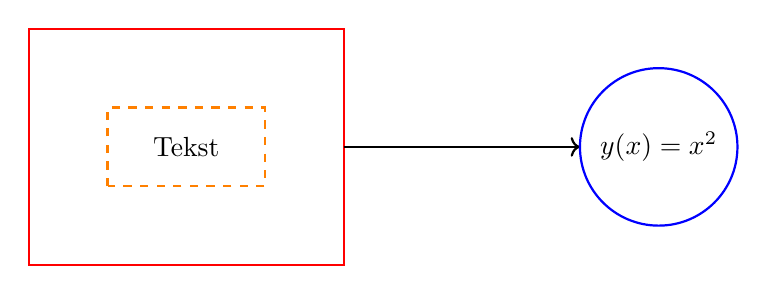
\begin{tikzpicture}
\draw [red, thick] (0,0) rectangle (4,3);
\draw [orange, thick,dashed] (1,1) rectangle (3,2);
\draw [->,thick] (4,1.5) -- (7,1.5);
\draw [blue, thick] (8,1.5) circle [radius=1];
\node at (2,1.5) {Tekst};
\node at (8,1.5) {$y(x)=x^2$};
\end{tikzpicture}
\end{figure}
\end{lstlisting}
pozwala narysowa? figury geometryczne przedstawione na rys. \ref{r_tikz_przyklad}. Zwr�?my uwag?, ?e napis oraz wz�r s? z?o?one aktualnie wykorzystywan? czcionk?, jej wielko?? jest taka sama jak w~ca?ym dokumencie.

\begin{figure}[b]
\centering
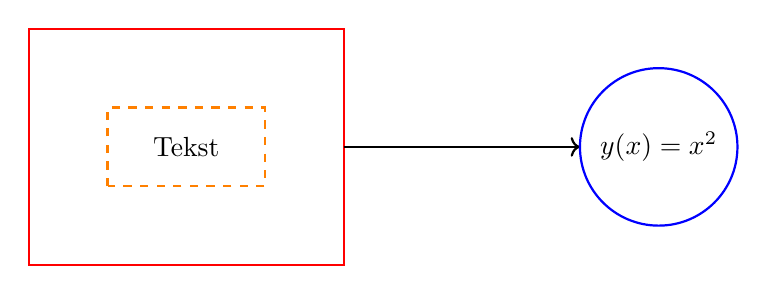
\begin{tikzpicture}
\draw [red, thick] (0,0) rectangle (4,3);
\draw [orange, thick,dashed] (1,1) rectangle (3,2);
\draw [->,thick] (4,1.5) -- (7,1.5);
\draw [blue, thick] (8,1.5) circle [radius=1];;
\node at (2,1.5) {Tekst};
\node at (8,1.5) {$y(x)=x^2$};
\end{tikzpicture}

\caption{Przyk?adowy rysunek wykonany w~j?zyku \texttt{TikZ/PGF}}
\label{r_tikz_przyklad}
\end{figure}

Przy wi?kszych rysunkach mo?na wykorzysta? programy umo?liwiaj?ce ich przygotowanie przy wykorzystaniu ?rodowiska graficznego, np. \verb+TikzEdt+ (\url{http://www.tikzedt.org/}), \verb+TpX+ (\url{http://tpx.sourceforge.net/}), \verb+ktikz+ (\url{https://www.linux-apps.com/p/1126914/}), \verb+GraTeX+ (\url{https://sourceforge.net/projects/gratex/}).

Mo?na r�wnie? wykorzysta? starsze, klasyczne pakiety \verb+picture+, \verb+epic+, \verb+eepic+. R�wnie? w~tych przypadkach mo?na ,,r?cznie'' opisywa? poszczeg�lne elementy graficzne lub skorzysta? ze ?rodowiska graficznego, np. \verb+LaTeXPiX+ (\url{http://latexpix.software.informer.com/}), kt�re znacznie przyspiesza prac?. Inne narz?dzia, umo?liwiaj?ce opracowanie rysunk�w wysokiej jako?ci, to \verb+METAPOST+ oraz \verb+PSTricks+.

\section{Kolory}
Przy umieszczaniu kilku wykres�w na tym samym rysunku, np. wynik�w eksperyment�w dla r�?nych warto?ci parametr�w, nale?y zastosowa? kolory r�?ni?ce si? od siebie w~znacznym stopniu, nie mo?na stosowa? kolor�w podobnych, np. kilku odcieni tego samego koloru. Warto zastosowa? standardow? palet? kolor�w o~nazwie \texttt{lines}, u?yt? w~pakiecie MATLAB, kt�ra zosta?a przedstawiona w~tab.~\ref{r_zestaw_kolorow}. Definicja tych kolor�w w~systemie \LaTeX\ jest nast?puj?ca:
\begin{lstlisting}[style=customlatex,frame=single]
\definecolor{niebieski}{rgb}{0,0.447,0.741}
\definecolor{czerwony}{rgb}{0.85,0.325,0.098}	
\definecolor{zolty}{rgb}{0.929,0.694,0.125}		
\definecolor{fioletowy}{rgb}{0.494,0.184,0.556}	
\definecolor{zielony}{rgb}{0.466,0.674,0.188}
\definecolor{jasnoniebieski}{rgb}{0.301,0.745,0.933}
\definecolor{ciemnioczerwony}{rgb}{0.635,0.078,0.184}
\end{lstlisting}

\definecolor{niebieski}{rgb}{0,0.447,0.741}
\definecolor{czerwony}{rgb}{0.85,0.325,0.098}	
\definecolor{zolty}{rgb}{0.929,0.694,0.125}		
\definecolor{fioletowy}{rgb}{0.494,0.184,0.556}	
\definecolor{zielony}{rgb}{0.466,0.674,0.188}
\definecolor{jasnoniebieski}{rgb}{0.301,0.745,0.933}
\definecolor{ciemnioczerwony}{rgb}{0.635,0.078,0.184}

\begin{table}[h]
\caption{Paleta 7 kolor�w}
\label{r_zestaw_kolorow}
	\centering
	\begin{small}
		\begin{tabular}{|p{3cm}|p{4cm}|}
			\hline
			%\multicolumn{1}{|c|}{Nazwa koloru\rule{0pt}{3.5mm}} & \multicolumn{1}{|c|}{} \\ \hline
			niebieski & \cellcolor{niebieski}\\
			czerwony & \cellcolor{czerwony}\\
			zolty & \cellcolor{zolty}\\
			fioletowy & \cellcolor{fioletowy}\\
			zielony & \cellcolor{zielony}\\
			jasnoniebieski & \cellcolor{jasnoniebieski}\\
			ciemnioczerwony & \cellcolor{ciemnioczerwony}\\
			\hline
		\end{tabular}
	\end{small}
\end{table}

\section{Funkcje statyczne}
Do wykonywania wykres�w prezentuj?cych wyniki symulacji i~eksperyment�w stosuje si? pakiet \verb+PGFPLOTS+ \cite{litFeuersanger2016}. Za?�?my, ?e w~katalogu \verb+rysunki/dane_stat+ znajduje si? plik \verb+dane_fx.txt+ zawieraj?cy w~pierwszej kolumnie warto?ci argumentu $x$, natomiast w~drugiej kolumnie warto?ci funkcji $f(x)$:
\begin{lstlisting}[style=customlatex,frame=single]
  -10.0000 -808.7350
   -9.0000 -696.4791
   -8.0000 -539.7850
   -7.0000 -386.1268
   -6.0000 -291.5881
   -5.0000 -267.6436
   -4.0000 -268.9551
   -3.0000 -233.3995
   -2.0000 -137.5303
   -1.0000  -16.4788
         0   70.0000
    1.0000   94.1212
    2.0000   87.2697
    3.0000  112.8005
    4.0000  209.4449
    5.0000  357.3564
    6.0000  498.0119
    7.0000  589.6732
    8.0000  647.4150
    9.0000  730.9209
   10.0000  891.2650
\end{lstlisting}
oraz podobny plik \verb+dane_gx.txt+, definiuj?cy funkcj? $g(x)$. Aby narysowa? te funkcje stosuje si? polecenia:
\begin{lstlisting}[style=customlatex,frame=single]
\newcommand{\szer}{8cm}
\newcommand{\wys}{7cm}

\begin{figure}[t]
\centering
\begin{tikzpicture}
\begin{axis}[
	width=\szer,
	height=\wys,
	xmin=-10,xmax=10,ymin=-1000,ymax=1000,
	xlabel={$x$},
	ylabel={$f(x), \ g(x)$},
	xtick={-10,-5,0,5,10},
	ytick={-1000,-500,0,500,1000},
	legend pos=south east,
]

\definecolor{niebieski}{rgb}{0,0.447,0.741}
\definecolor{czerwony}{rgb}{0.85,0.325,0.098}	

\addplot[niebieski,thick]
	file {rysunki/dane_stat/dane_fx.txt};
\addplot[czerwony,thick,densely dashed]
	file {rysunki/dane_stat/dane_gx.txt};
\legend{$f(x)$,$g(x)$}
\end{axis}
\end{tikzpicture}
\caption{Przyk?adowy rysunek funkcji $f(x)$ i~$g(x)$ wykonany 
w~j?zyku \texttt{PGFPLOTS}}
\label{r_pgfplots_funkcje}
\end{figure}
\end{lstlisting}
Otrzymany rezultat przedstawiono na rys.~\ref{r_pgfplots_funkcje}.

Dla wykorzystanej palety kolor�w ?adnie wygl?daj? rysunki o~pogrubionych liniach (styl \verb+thick+).

Istnieje mo?liwo?? ustawienia wielko?ci czcionek liczb umieszczonych: na osiach (\verb+tick label style+), w~oznaczeniach osi (\verb+label style+), w~legendzie (\verb+legend style+) oraz w~tytule rysunku (\verb+title style+). Przyk?adowa konfiguracja zmieniaj?ca wielko?? czcionek jest nast?puj?ca:
\begin{lstlisting}[style=customlatex,frame=single]
\pgfplotsset{
	tick label style={font=\tiny},
	label style={font=\footnotesize},
	legend style={font=\footnotesize},
	title style={font=\footnotesize},
	/pgf/number format/.cd, use comma, 1000 sep={}
}
\end{lstlisting}
Dodatkowo, sekwencja \verb+/pgf/number format/.cd, use comma, 1000 sep={}+ ustawia przecinek jako separator dziesi?tny (zamiast domy?lnej kropki) oraz kasuje separator, oddzielaj?cy tysi?ce od setek (domy?lenie jest to przecinek).

\newcommand{\szer}{8cm}
\newcommand{\wys}{7cm}

\begin{figure}[tb]
\centering
\begin{tikzpicture}
\begin{axis}[
	width=\szer,
	height=\wys,
	xmin=-10,xmax=10,ymin=-1000,ymax=1000,
	xlabel={$x$},
	ylabel={$f(x), \ g(x)$},
	xtick={-10,-5,0,5,10},
	ytick={-1000,-500,0,500,1000},
	legend pos=south east,
]

\definecolor{niebieski}{rgb}{0,0.447,0.741}
\definecolor{czerwony}{rgb}{0.85,0.325,0.098}	

\addplot[niebieski,thick]
	file {rysunki/dane_stat/dane_fx.txt};
\addplot[czerwony,thick,densely dashed]
	file {rysunki/dane_stat/dane_gx.txt};
\legend{$f(x)$,$g(x)$}
\end{axis}
\end{tikzpicture}
\caption{Przyk?adowy rysunek funkcji $f(x)$ i~$g(x)$ wykonany w~j?zyku \texttt{PGFPLOTS} (rysunek jest generowany przy ka?dym przetworzenia pliku ?r�d?owego}
\label{r_pgfplots_funkcje}
\end{figure}

Opisany spos�b implementacji rysunk�w jest poprawny, ale ma powa?n? wad?, poniewa? \LaTeX{}   potrzebuje do?? du?o czasu na ich przetworzenie. Okazuje si? to du?ym mankamentem szczeg�lnie w�wczas, gdy w~dokumencie znajduje si? du?o skomplikowanych rysunk�w. Skutecznym rozwi?zaniem jest przygotowanie rysunk�w i~zapis ich do plik�w \verb+pdf+, a~nast?pnie do??czenie ich do g?�wnego dokumentu poleceniem \verb+\includegraphics+. W~katalogu \verb+rysunki/zapisz_pdf+ podano kilka przyk?ad�w takich rysunk�w. Plik ?r�d?owy \verb+funkcje.tex+ ma posta?:
\lstinputlisting[style=customlatex,frame=single]{rysunki/zapisz_pdf/funkcje.tex}
Zwr�?my uwag?, ?e dzi?ki zastosowaniu klasy \verb+standalone+, wygenerowany zostanie rysunek o~zadanych wymiarach (bez niepotrzebych margines�w), plik \verb+pdf+ nie b?dzie formatu A4. Nast?puj?ce polecenie 
\begin{lstlisting}[style=customlatex,frame=single]
pdflatex funkcje.tex
\end{lstlisting}
zapisuje plik \verb+funkcje.pdf+. Wygenerowany rysunek do??cza si? do dokumentu ci?giem instrukcji:
\begin{lstlisting}[style=customlatex,frame=single]
\begin{figure}[tb]
\centering
\includegraphics[scale=1]{pgfplots_pdf/funkcje}
\caption{Przyk?adowy rysunek funkcji $f(x)$ i~$g(x)$ wykonany
w~j?zyku \texttt{PGFPLOTS}}
\label{r_pgfplots_funkcje}
\end{figure}
\end{lstlisting}
Otrzymany rezultat przedstawiono na rys.~\ref{r_pgfplots_funkcje_pdf}. Oczywi?cie, rysunki \ref{r_pgfplots_funkcje} i~\ref{r_pgfplots_funkcje_pdf} s? bardzo podobne, inna jest tylko wielko?? czcionek na osiach.

Przy du?ych zbiorach danych \LaTeX{} zg?asza b??d pami?ci. Nale?y w�wczas zastosowa? system sk?adu \hbox{Lua\LaTeX}.

Nie nale?y skalowa? rysunku przy wykorzystaniu argument�w polecenia \verb+\includegraphics+, gdy? zmieni to wielko?? zastosowanej czcionki. Je?eli zachodzi konieczno?? zmiany wielko?ci rysunku, nale?y zmodyfikowa? plik ?r�d?owy generuj?cy rysunek.

Je?eli rysunek jest znacznie szerszy ni? szeroko?? strony (oraz gdy nie mo?emy lub nie chcemy redukowa? szeroko?ci rysunku), nale?y zastosowa? otoczenie \verb+sidewaysfigure+ z~pakietu \verb+rotating+, kt�re dzia?a analogicznie jak otoczenie \verb+sidewaystable+.

W~dokumentacji pakietu \verb+PGFPLOTS+ om�wiono spos�b przygotowania rysunk�w tr�jwymiarowych \cite{litFeuersanger2016}.

\begin{figure}[ptb]
\centering
\includegraphics[scale=1]{rysunki/zapisz_pdf/funkcje}
\caption{Przyk?adowy rysunek funkcji $f(x)$ i~$g(x)$ wykonany
w~j?zyku \texttt{PGFPLOTS} i~zapisany w~pliku \texttt{funkcje.pdf}}
\label{r_pgfplots_funkcje_pdf}
\end{figure}

\section{Wyniki symulacji i~eksperyment�w}
\subsection{Procesy jednowymiarowe}
Za?�?my, ?e w~katalogu \verb+rysunki/symulacje11+ znajduje si? plik \verb+yzad.txt+ zawieraj?cy w~pierwszej kolumnie pomiary czasu $t$ (w~sekundach), natomiast w~drugiej kolumnie pr�bki sygna?u warto?ci zadanej $y^{\mathrm{zad}}$. Wykonano symulacje algorytmu regulacji GPC przy pi?ciu r�?nych warto?ciach parametru $\lambda$: $\num{0,1}$, $\num{0,2}$, $\num{0,5}$, $\num{1}$ i~$\num{2}$. Przebiegi sygna?u steruj?cego $u$ zapisano w~plikach \verb+u_lambda_0_1.txt+, \verb+u_lambda_0_2.txt+, \verb+u_lambda_0_5.txt+, \verb+u_lambda_1.txt+ i~\verb+u_lambda_2.txt+, natomiast przebiegi sygna?u wyj?ciowego procesu $y$ zapisano w~plikach \verb+y_lambda_0_1.txt+, \verb+y_lambda_0_2.txt+, \verb+y_lambda_0_5.txt+, \verb+y_lambda_1.txt+ i~\verb+y_lambda_2.txt+. Przygotowano plik \verb+symulacje11.tex+, umo?liwiaj?cy zapisanie rysunku do pliku \verb+symulacje11.pdf+. Znajduje si? on w~katalogu \verb+rysunki/zapisz_pdf+ i~ma nast?puj?c? posta?:
\lstinputlisting[style=customlatex,frame=single]{rysunki/zapisz_pdf/symulacje11.tex}
Na pocz?tku powy?szego pliku zostaje wczytany i~skonfigurowany pakiet \verb+siunitx+. Mi?dzy innymi, ustawiamy przecinek jako separator dziesi?tny. Liczby z~cz??ci? u?amkow? zapisujemy w~postaci \verb+\num{0.1}+. W~zale?no?ci od konfiguracji, otrzymamy $0.1$ lub $0{,}1$. Polecenie
\begin{lstlisting}[style=customlatex,frame=single]
pdflatex symulacje11.tex
\end{lstlisting}
zapisuje plik \verb+symulacje11.pdf+. Rezultat przedstawiono na rys.~\ref{r_pgfplots_symulacje11_pdf}. Rysunek do??cza si? do dokumentu instrukcj? \verb+\includegraphics+. Zwr�?my uwag?, ?e do narysowania wynik�w symulacji dla kolejnych warto?ci parametru $\lambda$ zastosowano r�?ne kolory oraz r�?ne style linii (linia ci?g?a, linia przerywana, itd.). Umo?liwia to ?atwe rozr�?nienie dokument�w na czarno-bia?ym wydruku. Przy wydruku kolorowym oraz dokumentach elektronicznych mo?na zrezygnowa? ze stosowania r�?nych styl�w linii, do ich rozr�?nienia wystarczaj?ce s? kolory, pod warunkiem jednak, ?e kolejne krzywe nie s? po?o?one bardzo blisko siebie.

Czasami, ze wzgl?du na ograniczon? obj?to?? dokumentu, nale?y zmniejszy? rysunki. Aby zmniejszy? obj?to?? mo?na zastosowa? u?o?enie poziome dw�ch rysunk�w, prezentuj?cych wyniki symulacji procesu. Przygotowano plik \verb+symulacje11_wersja2.tex+, umo?liwiaj?cy zapisanie rysunku do pliku \verb+symulacje11_wersja2.pdf+. Znajduje si? on w~katalogu \verb+rysunki/zapisz_pdf+ i~ma nast?puj?c? posta?:
\lstinputlisting[style=customlatex,frame=single]{rysunki/zapisz_pdf/symulacje11_wersja2.tex}
Rezultat przedstawiono na rys.~\ref{r_pgfplots_symulacje11_wersja2_pdf}.

\begin{figure}[H]
\centering
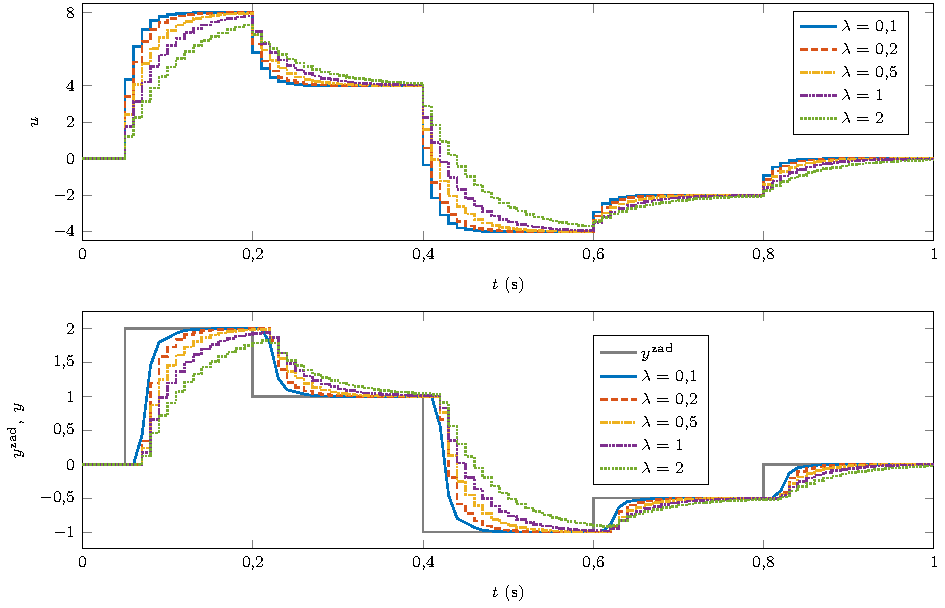
\includegraphics[scale=1]{rysunki/zapisz_pdf/symulacje11}
%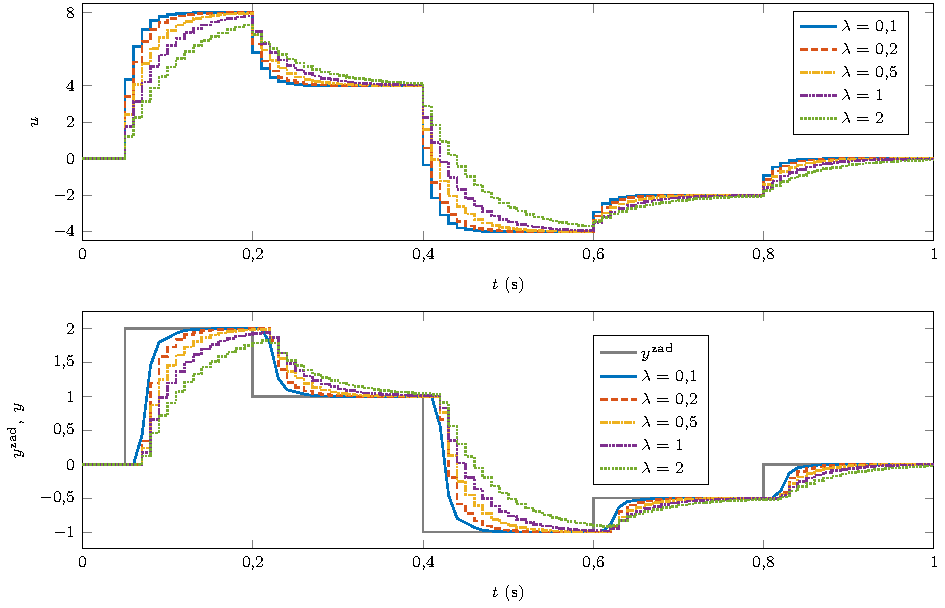
\includegraphics[scale=1]{rysunki/zapisz_pdf/symulacje11}
\caption{Przyk?adowy rysunek wynik�w symulacji procesu jednowymiarowego wykonany
w~j?zyku \texttt{PGFPLOTS} i~zapisany w~pliku \texttt{symulacje11.pdf}}
\label{r_pgfplots_symulacje11_pdf}
\end{figure}

\begin{figure}[H]
\centering
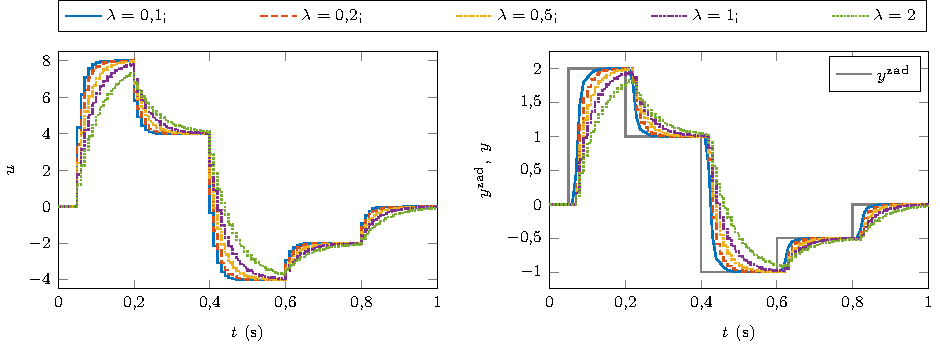
\includegraphics[scale=1]{rysunki/zapisz_pdf/symulacje11_wersja2}
\caption{Przyk?adowy rysunek wynik�w symulacji procesu jednowymiarowego wykonany
w~j?zyku \texttt{PGFPLOTS} i~zapisany w~pliku \texttt{symulacje11\_wersja2.pdf}}
\label{r_pgfplots_symulacje11_wersja2_pdf}
\end{figure}

\subsection{Procesy wielowymiarowe}
Za?�?my, ?e w~katalogu \verb+rysunki/symulacje22+ znajduj? si? wyniki symulacji procesu o~dw�ch wej?ciach i~dw�ch wyj?ciach zapisane w~plikach: \verb+yzad1.txt+, \verb+yzad2.txt+, \verb+u1.txt+, \verb+u2.txt+, \verb+y1.txt+, \verb+y2.txt+. W~pierwszej kolumnie tych plik�w podano czas $t$ (w~sekundach), natomiast w~drugiej kolumnie warto?? odpowiedniej zmiennej. Plik \verb+symulacje22.tex+, umo?liwiaj?cy zapisanie rysunku do pliku \verb+symulacje22.pdf+ znajduje si? w~katalogu \verb+rysunki/zapisz_pdf+ i~ma nast?puj?c? posta?:
\lstinputlisting[style=customlatex,frame=single]{rysunki/zapisz_pdf/symulacje22.tex}
Rezultat przedstawiono na rys.~\ref{r_pgfplots_symulacje22_pdf}.

Aby zmniejszy? obj?to?? mo?na nieco inaczej u?o?y? 4 rysunki, prezentuj?ce wyniki symulacji procesu dwuwymiarowego. Przygotowano plik \verb+symulacje22_wersja2.tex+, umo?liwiaj?cy zapisanie rysunku do pliku \verb+symulacje22_wersja2.pdf+. Znajduje si? on w~katalogu \verb+rysunki/zapisz_pdf+ i~ma nast?puj?c? posta?:
\lstinputlisting[style=customlatex,frame=single]{rysunki/zapisz_pdf/symulacje22_wersja2.tex}
Rezultat przedstawiono na rys.~\ref{r_pgfplots_symulacje22_wersja2_pdf}.

\begin{figure}[H]
\centering
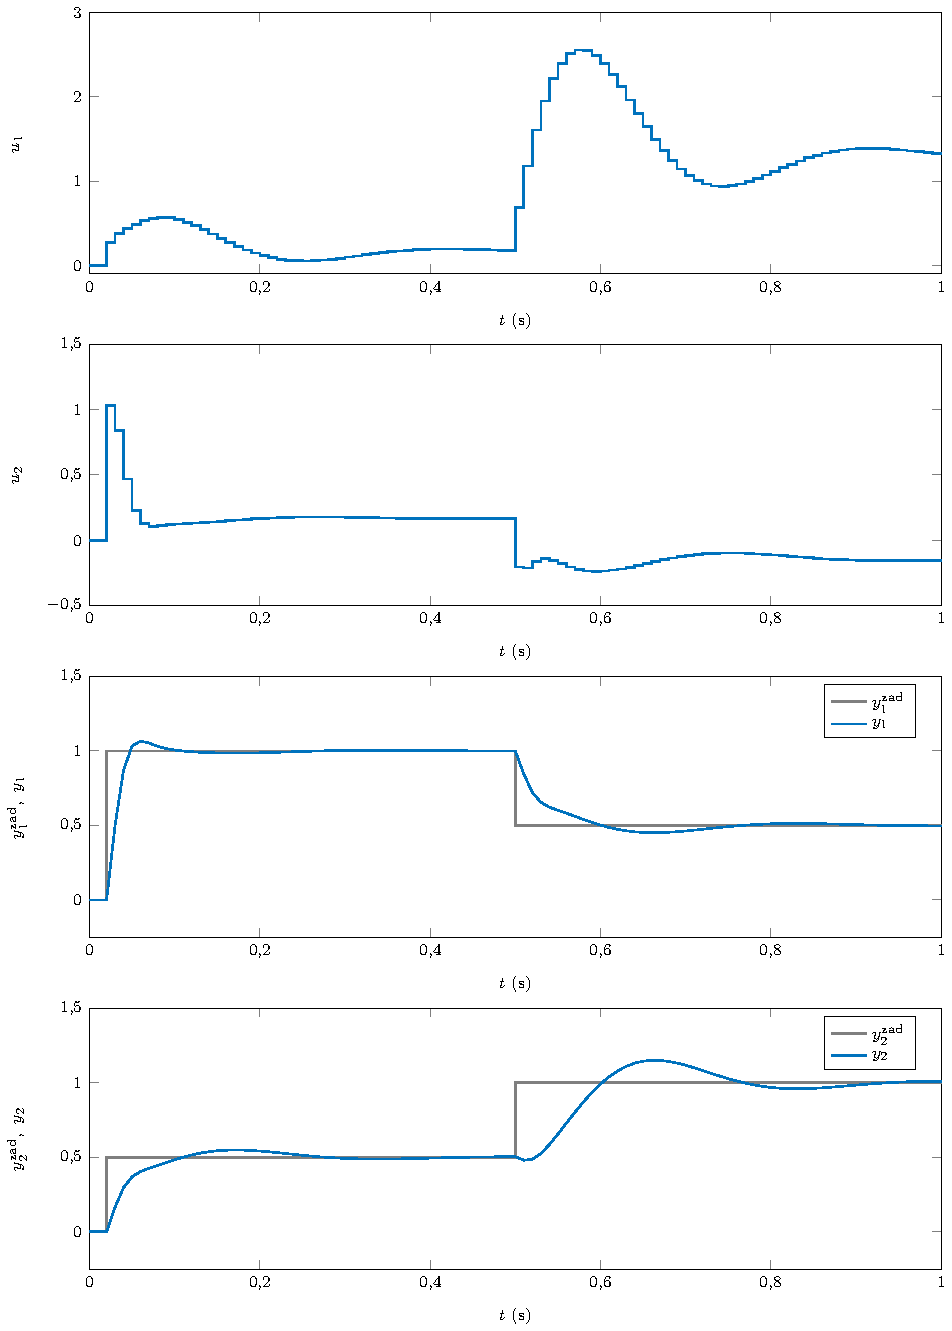
\includegraphics[scale=1]{rysunki/zapisz_pdf/symulacje22}
\caption{Przyk?adowy rysunek wynik�w symulacji procesu dwuwymiarowego wykonany
w~j?zyku \texttt{PGFPLOTS} i~zapisany w~pliku \texttt{symulacje22.pdf}}
\label{r_pgfplots_symulacje22_pdf}
\end{figure}

\begin{figure}[H]
\centering
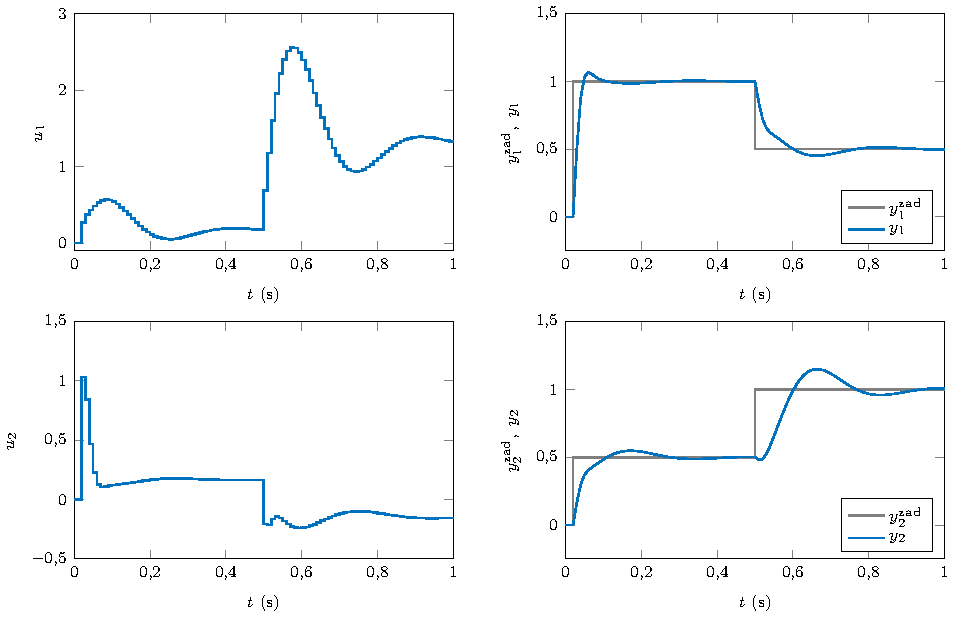
\includegraphics[scale=1]{rysunki/zapisz_pdf/symulacje22_wersja2}
\caption{Przyk?adowy rysunek wynik�w symulacji procesu dwuwymiarowego wykonany
w~j?zyku \texttt{PGFPLOTS} i~zapisany w~pliku \texttt{symulacje22\_wersja2.pdf}}
\label{r_pgfplots_symulacje22_wersja2_pdf}
\end{figure}

\section{Zapis wielu rysunk�w do jednego pliku \texttt{pdf}}
Aktywacja klasy \verb+standalone+ z~opcj? \verb+tikz+ umo?liwia zapis wielu rysunk�w do jednego pliku \texttt{pdf}. Rozwa?my przyk?adowy plik \verb+funkcje2.tex+ z~katalogu \verb+rysunki/zapisz_pdf+:
\lstinputlisting[style=customlatex,frame=single]{rysunki/zapisz_pdf/funkcje2.tex}
Ka?dy rysunek wygenerowany przez otoczenie \verb+tikzpicture+ znajdzie si? na osobnej stronie. Co wa?ne, je?eli ka?dy rysunek b?dzie mia? inne wymiary, dzi?ki klasie \verb+standalone+ ka?da strona jest przycinana do zawarto?ci. Gotowe rysunki wstawiamy do dokumentu poleceniami (oczywi?cie w~otoczeniu \verb+figure+):
\begin{lstlisting}[style=customlatex,frame=single]
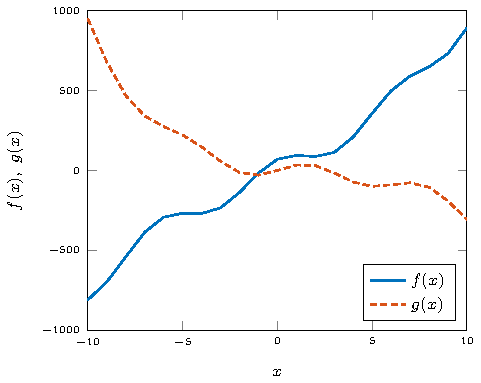
\includegraphics[page=1]{funkcje2.pdf}
\end{lstlisting}
oraz
\begin{lstlisting}[style=customlatex,frame=single]
\includegraphics[page=2]{funkcje2.pdf}
\end{lstlisting}
Opisany spos�b zapisu rysunk�w pozwala na ograniczenie liczby plik�w oraz umo?liwia grupowanie tre?ci.

\section{Prosty eksport wykres�w: skrypt \texttt{matlab2tikz}}
Opr�cz opisanego sposobu przygotowywania rysunk�w z~wykorzystaniem pakietu \verb+PGFPLOTS+, mo?na wykorzysta? skrypt \texttt{matlab2tikz}, kt�ry generuje kod ?r�d?owy (\verb+TikZ+) rysunku wykonanego w~programie MATLAB. Skrypt \texttt{matlab2tikz} dost?pny jest pod adresem: \url{https://www.mathworks.com/matlabcentral/fileexchange/22022-matlab2tikz-matlab2tikz}. Rozwa?my przyk?adowy plik \verb+wykresy_z_matlaba.m+ z~katalogu \verb+rysunki/matlab2tikz+:
\lstinputlisting[style=Matlab-editor]{./rysunki/matlab2tikz/wykresy_z_matlaba.m}
Wykres wstawiamy do dokumentu w~nst?puj?cy spos�b:
\begin{lstlisting}[style=customlatex,frame=single]
\begin{figure}[H]
\centering
	% This file was created by matlab2tikz.
%
\definecolor{mycolor1}{rgb}{0.00000,0.44700,0.74100}%
%
\begin{tikzpicture}

\begin{axis}[%
width=4.521in,
height=3.566in,
at={(0.758in,0.481in)},
scale only axis,
xmin=0,
xmax=3.141,
xlabel style={font=\color{white!15!black}},
xlabel={$x$},
ymin=-1,
ymax=1,
ylabel style={font=\color{white!15!black}},
ylabel={$y$},
axis background/.style={fill=white},
legend style={legend cell align=left, align=left, draw=white!15!black}
]
\addplot [color=mycolor1, line width=1.0pt]
  table[row sep=crcr]{%
0	0\\
0.001	2e-12\\
0.002	3.2e-11\\
0.003	1.62e-10\\
0.004	5.12e-10\\
0.005	1.25e-09\\
0.006	2.592e-09\\
0.007	4.802e-09\\
0.008	8.192e-09\\
0.009	1.3122e-08\\
0.01	2e-08\\
0.011	2.9282e-08\\
0.012	4.1472e-08\\
0.013	5.7122e-08\\
0.014	7.68319999999999e-08\\
0.015	1.0125e-07\\
0.016	1.31072e-07\\
0.017	1.67041999999999e-07\\
0.018	2.09951999999999e-07\\
0.019	2.60641999999997e-07\\
0.02	3.19999999999995e-07\\
0.021	3.8896199999999e-07\\
0.022	4.68511999999983e-07\\
0.023	5.59681999999971e-07\\
0.024	6.63551999999951e-07\\
0.025	7.81249999999921e-07\\
0.026	9.13951999999873e-07\\
0.027	1.0628819999998e-06\\
0.028	1.22931199999969e-06\\
0.029	1.41456199999953e-06\\
0.03	1.61999999999929e-06\\
0.031	1.84704199999895e-06\\
0.032	2.09715199999846e-06\\
0.033	2.37184199999778e-06\\
0.034	2.67267199999682e-06\\
0.035	3.0012499999955e-06\\
0.036	3.35923199999368e-06\\
0.037	3.74832199999122e-06\\
0.038	4.17027199998791e-06\\
0.039	4.62688199998349e-06\\
0.04	5.11999999997763e-06\\
0.041	5.65152199996992e-06\\
0.042	6.22339199995983e-06\\
0.043	6.83760199994672e-06\\
0.044	7.49619199992979e-06\\
0.045	8.20124999990806e-06\\
0.046	8.95491199988032e-06\\
0.047	9.75936199984508e-06\\
0.048	1.06168319998006e-05\\
0.049	1.15296019997446e-05\\
0.05	1.24999999996745e-05\\
0.051	1.35304019995872e-05\\
0.052	1.46232319994788e-05\\
0.053	1.5780961999345e-05\\
0.054	1.70061119991803e-05\\
0.055	1.83012499989784e-05\\
0.056	1.96689919987318e-05\\
0.057	2.11120019984317e-05\\
0.058	2.26329919980677e-05\\
0.059	2.42347219976277e-05\\
0.06	2.59199999970976e-05\\
0.061	2.76916819964609e-05\\
0.062	2.95526719956983e-05\\
0.063	3.15059219947878e-05\\
0.064	3.35544319937035e-05\\
0.065	3.5701249992416e-05\\
0.066	3.79494719908911e-05\\
0.067	4.03022419890897e-05\\
0.068	4.2762751986967e-05\\
0.069	4.53342419844716e-05\\
0.07	4.8019999981545e-05\\
0.071	5.08233619781204e-05\\
0.072	5.37477119741221e-05\\
0.073	5.67964819694639e-05\\
0.074	5.99731519640483e-05\\
0.075	6.32812499577649e-05\\
0.076	6.6724351950489e-05\\
0.077	7.03060819420801e-05\\
0.078	7.40301119323802e-05\\
0.079	7.79001619212113e-05\\
0.08	8.1919999908374e-05\\
0.081	8.60934418936448e-05\\
0.082	9.04243518767733e-05\\
0.083	9.491664185748e-05\\
0.084	9.9574271835453e-05\\
0.085	0.000104401249810344\\
0.086	0.000109401631781767\\
0.087	0.000114579521749291\\
0.088	0.000119939071712438\\
0.089	0.000125484481670679\\
0.09	0.000131219999623427\\
0.091	0.000137149921570033\\
0.092	0.000143278591509778\\
0.093	0.000149610401441872\\
0.094	0.00015614979136544\\
0.095	0.00016290124927952\\
0.096	0.000169869311183054\\
0.097	0.000177058561074877\\
0.098	0.000184473630953711\\
0.099	0.000192119200818154\\
0.1	0.000199999998666667\\
0.101	0.000208120800497567\\
0.102	0.000216486430309011\\
0.103	0.000225101760098986\\
0.104	0.00023397170986529\\
0.105	0.000243101247605525\\
0.106	0.000252495389317071\\
0.107	0.000262159198997078\\
0.108	0.00027209778864244\\
0.109	0.00028231631824978\\
0.11	0.000292819995815429\\
0.111	0.000303614077335399\\
0.112	0.000314703866805365\\
0.113	0.000326094716220636\\
0.114	0.000337792025576127\\
0.115	0.000349801242866333\\
0.116	0.000362127864085297\\
0.117	0.000374777433226577\\
0.118	0.00038775554228321\\
0.119	0.000401067831247678\\
0.12	0.000414719988111866\\
0.121	0.000428717748867023\\
0.122	0.000443066897503716\\
0.123	0.000457773266011782\\
0.124	0.000472842734380282\\
0.125	0.000488281230597447\\
0.126	0.00050409473065062\\
0.127	0.000520289258526201\\
0.128	0.000536870886209583\\
0.129	0.000553845733685086\\
0.13	0.000571219968935887\\
0.131	0.00058899980794395\\
0.132	0.000607191514689944\\
0.133	0.000625801401153164\\
0.134	0.000644835827311446\\
0.135	0.00066430120114107\\
0.136	0.000684203978616674\\
0.137	0.000704550663711144\\
0.138	0.000725347808395512\\
0.139	0.000746602012638843\\
0.14	0.000768319924408119\\
0.141	0.000790508239668112\\
0.142	0.000813173702381256\\
0.143	0.000836323104507509\\
0.144	0.000859963286004208\\
0.145	0.000884101134825921\\
0.146	0.000908743586924287\\
0.147	0.000933897626247844\\
0.148	0.000959570284741863\\
0.149	0.000985768642348157\\
0.15	0.00101249982700489\\
0.151	0.00103977101464638\\
0.152	0.00106758942920289\\
0.153	0.00109596234260038\\
0.154	0.0011248970747603\\
0.155	0.00115440099359937\\
0.156	0.00118448151502926\\
0.157	0.00121514610295639\\
0.158	0.00124640226928159\\
0.159	0.00127825757389986\\
0.16	0.00131071962470006\\
0.161	0.00134379607756456\\
0.162	0.00137749463636891\\
0.163	0.00141182305298153\\
0.164	0.00144678912726332\\
0.165	0.00148240070706727\\
0.166	0.00151866568823811\\
0.167	0.00155559201461181\\
0.168	0.00159318767801526\\
0.169	0.00163146071826574\\
0.17	0.00167041922317046\\
0.171	0.00171007132852611\\
0.172	0.00175042521811833\\
0.173	0.00179148912372115\\
0.174	0.00183327132509648\\
0.175	0.00187578014999352\\
0.176	0.00191902397414814\\
0.177	0.0019630112212823\\
0.178	0.00200775036310335\\
0.179	0.00205324991930337\\
0.18	0.0020995184575585\\
0.181	0.00214656459352815\\
0.182	0.0021943969908543\\
0.183	0.00224302436116064\\
0.184	0.00229245546405183\\
0.185	0.00234269910711257\\
0.186	0.00239376414590674\\
0.187	0.00244565948397651\\
0.188	0.00249839407284133\\
0.189	0.00255197691199696\\
0.19	0.00260641704891444\\
0.191	0.00266172357903902\\
0.192	0.00271790564578901\\
0.193	0.00277497244055471\\
0.194	0.00283293320269711\\
0.195	0.00289179721954672\\
0.196	0.00295157382640227\\
0.197	0.00301227240652934\\
0.198	0.00307390239115904\\
0.199	0.00313647325948651\\
0.2	0.00319999453866946\\
0.201	0.00326447580382667\\
0.202	0.00332992667803632\\
0.203	0.00339635683233439\\
0.204	0.00346377598571297\\
0.205	0.00353219390511842\\
0.206	0.00360162040544959\\
0.207	0.00367206534955594\\
0.208	0.00374353864823551\\
0.209	0.00381605026023294\\
0.21	0.0038896101922374\\
0.211	0.00396422849888034\\
0.212	0.0040399152827333\\
0.213	0.00411668069430558\\
0.214	0.00419453493204182\\
0.215	0.00427348824231956\\
0.216	0.00435355091944663\\
0.217	0.00443473330565855\\
0.218	0.00451704579111574\\
0.219	0.00460049881390075\\
0.22	0.0046851028600153\\
0.221	0.0047708684633773\\
0.222	0.00485780620581768\\
0.223	0.00494592671707728\\
0.224	0.00503524067480342\\
0.225	0.00512575880454656\\
0.226	0.00521749187975673\\
0.227	0.00531045072177991\\
0.228	0.00540464619985424\\
0.229	0.00550008923110619\\
0.23	0.00559679078054652\\
0.231	0.00569476186106618\\
0.232	0.00579401353343207\\
0.233	0.00589455690628261\\
0.234	0.00599640313612328\\
0.235	0.00609956342732195\\
0.236	0.00620404903210408\\
0.237	0.00630987125054774\\
0.238	0.00641704143057859\\
0.239	0.0065255709679646\\
0.24	0.00663547130631062\\
0.241	0.00674675393705287\\
0.242	0.00685943039945317\\
0.243	0.00697351228059307\\
0.244	0.00708901121536776\\
0.245	0.00720593888647983\\
0.246	0.00732430702443283\\
0.247	0.00744412740752466\\
0.248	0.00756541186184074\\
0.249	0.00768817226124705\\
0.25	0.00781242052738283\\
0.251	0.00793816862965327\\
0.252	0.0080654285852218\\
0.253	0.0081942124590023\\
0.254	0.00832453236365099\\
0.255	0.00845640045955818\\
0.256	0.00858982895483971\\
0.257	0.00872483010532821\\
0.258	0.00886141621456407\\
0.259	0.00899959963378621\\
0.26	0.00913939276192254\\
0.261	0.0092808080455802\\
0.262	0.00942385797903552\\
0.263	0.00956855510422371\\
0.264	0.00971491201072822\\
0.265	0.00986294133576994\\
0.266	0.0100126557641959\\
0.267	0.010164068028468\\
0.268	0.0103171909086509\\
0.269	0.0104720372324002\\
0.27	0.01062861987495\\
0.271	0.0107869517591001\\
0.272	0.0109470458552027\\
0.273	0.0111089151811493\\
0.274	0.0112725728023569\\
0.275	0.0114380318317536\\
0.276	0.0116053054297642\\
0.277	0.0117744068042955\\
0.278	0.0119453492107209\\
0.279	0.0121181459518647\\
0.28	0.0122928103779861\\
0.281	0.0124693558867626\\
0.282	0.0126477959232734\\
0.283	0.0128281439799819\\
0.284	0.0130104135967178\\
0.285	0.0131946183606594\\
0.286	0.0133807719063144\\
0.287	0.0135688879155009\\
0.288	0.0137589801173282\\
0.289	0.0139510622881763\\
0.29	0.0141451482516756\\
0.291	0.0143412518786853\\
0.292	0.0145393870872728\\
0.293	0.0147395678426904\\
0.294	0.0149418081573536\\
0.295	0.0151461220908174\\
0.296	0.0153525237497526\\
0.297	0.0155610272879214\\
0.298	0.0157716469061529\\
0.299	0.0159843968523168\\
0.3	0.016199291421298\\
0.301	0.0164163449549695\\
0.302	0.016635571842165\\
0.303	0.0168569865186509\\
0.304	0.0170806034670978\\
0.305	0.0173064372170508\\
0.306	0.0175345023448996\\
0.307	0.0177648134738481\\
0.308	0.0179973852738821\\
0.309	0.018232232461738\\
0.31	0.0184693698008692\\
0.311	0.018708812101413\\
0.312	0.0189505742201554\\
0.313	0.0191946710604966\\
0.314	0.0194411175724146\\
0.315	0.019689928752428\\
0.316	0.0199411196435591\\
0.317	0.0201947053352945\\
0.318	0.0204507009635464\\
0.319	0.0207091217106115\\
0.32	0.0209699828051309\\
0.321	0.0212332995220467\\
0.322	0.0214990871825599\\
0.323	0.0217673611540862\\
0.324	0.0220381368502108\\
0.325	0.0223114297306423\\
0.326	0.0225872553011664\\
0.327	0.0228656291135973\\
0.328	0.0231465667657287\\
0.329	0.0234300839012842\\
0.33	0.0237161962098655\\
0.331	0.0240049194269004\\
0.332	0.0242962693335895\\
0.333	0.0245902617568515\\
0.334	0.0248869125692673\\
0.335	0.0251862376890236\\
0.336	0.0254882530798541\\
0.337	0.025792974750981\\
0.338	0.0261004187570534\\
0.339	0.0264106011980864\\
0.34	0.0267235382193973\\
0.341	0.0270392460115412\\
0.342	0.0273577408102455\\
0.343	0.0276790388963422\\
0.344	0.0280031565956998\\
0.345	0.0283301102791529\\
0.346	0.028659916362431\\
0.347	0.0289925913060853\\
0.348	0.0293281516154147\\
0.349	0.0296666138403894\\
0.35	0.0300079945755738\\
0.351	0.0303523104600472\\
0.352	0.0306995781773232\\
0.353	0.0310498144552675\\
0.354	0.0314030360660139\\
0.355	0.0317592598258788\\
0.356	0.0321185025952735\\
0.357	0.0324807812786157\\
0.358	0.032846112824238\\
0.359	0.0332145142242958\\
0.36	0.0335860025146725\\
0.361	0.0339605947748833\\
0.362	0.0343383081279769\\
0.363	0.0347191597404353\\
0.364	0.0351031668220718\\
0.365	0.0354903466259267\\
0.366	0.0358807164481612\\
0.367	0.0362742936279496\\
0.368	0.0366710955473681\\
0.369	0.0370711396312835\\
0.37	0.0374744433472378\\
0.371	0.0378810242053317\\
0.372	0.0382908997581055\\
0.373	0.0387040876004181\\
0.374	0.0391206053693231\\
0.375	0.039540470743943\\
0.376	0.0399637014453409\\
0.377	0.0403903152363897\\
0.378	0.0408203299216389\\
0.379	0.0412537633471791\\
0.38	0.0416906334005037\\
0.381	0.0421309580103677\\
0.382	0.042574755146645\\
0.383	0.0430220428201818\\
0.384	0.0434728390826478\\
0.385	0.0439271620263849\\
0.386	0.0443850297842529\\
0.387	0.0448464605294721\\
0.388	0.0453114724754634\\
0.389	0.0457800838756853\\
0.39	0.0462523130234681\\
0.391	0.0467281782518449\\
0.392	0.0472076979333795\\
0.393	0.0476908904799913\\
0.394	0.0481777743427773\\
0.395	0.0486683680118303\\
0.396	0.0491626900160545\\
0.397	0.0496607589229772\\
0.398	0.0501625933385575\\
0.399	0.0506682119069916\\
0.4	0.0511776333105147\\
0.401	0.0516908762691989\\
0.402	0.0522079595407483\\
0.403	0.0527289019202897\\
0.404	0.0532537222401603\\
0.405	0.0537824393696914\\
0.406	0.0543150722149882\\
0.407	0.0548516397187058\\
0.408	0.0553921608598218\\
0.409	0.055936654653404\\
0.41	0.0564851401503751\\
0.411	0.0570376364372725\\
0.412	0.0575941626360049\\
0.413	0.0581547379036033\\
0.414	0.0587193814319697\\
0.415	0.0592881124476193\\
0.416	0.0598609502114204\\
0.417	0.0604379140183283\\
0.418	0.0610190231971154\\
0.419	0.061604297110097\\
0.42	0.0621937551528516\\
0.421	0.0627874167539374\\
0.422	0.0633853013746035\\
0.423	0.0639874285084965\\
0.424	0.064593817681362\\
0.425	0.0652044884507415\\
0.426	0.0658194604056638\\
0.427	0.0664387531663317\\
0.428	0.067062386383803\\
0.429	0.067690379739667\\
0.43	0.0683227529457151\\
0.431	0.0689595257436061\\
0.432	0.069600717904526\\
0.433	0.0702463492288426\\
0.434	0.0708964395457539\\
0.435	0.0715510087129313\\
0.436	0.0722100766161566\\
0.437	0.0728736631689536\\
0.438	0.0735417883122132\\
0.439	0.074214472013813\\
0.44	0.0748917342682305\\
0.441	0.0755735950961501\\
0.442	0.0762600745440638\\
0.443	0.0769511926838659\\
0.444	0.0776469696124407\\
0.445	0.0783474254512441\\
0.446	0.0790525803458785\\
0.447	0.0797624544656606\\
0.448	0.080477068003183\\
0.449	0.0811964411738686\\
0.45	0.0819205942155179\\
0.451	0.0826495473878495\\
0.452	0.0833833209720333\\
0.453	0.0841219352702161\\
0.454	0.0848654106050408\\
0.455	0.0856137673191571\\
0.456	0.086367025774725\\
0.457	0.0871252063529112\\
0.458	0.0878883294533765\\
0.459	0.088656415493757\\
0.46	0.0894294849091359\\
0.461	0.090207558151508\\
0.462	0.0909906556892357\\
0.463	0.0917787980064971\\
0.464	0.0925720056027257\\
0.465	0.0933702989920407\\
0.466	0.0941736987026704\\
0.467	0.0949822252763652\\
0.468	0.0957958992678033\\
0.469	0.0966147412439859\\
0.47	0.097438771783625\\
0.471	0.098268011476521\\
0.472	0.0991024809229309\\
0.473	0.0999422007329285\\
0.474	0.100787191525753\\
0.475	0.101637473929151\\
0.476	0.102493068578704\\
0.477	0.103353996117152\\
0.478	0.104220277193702\\
0.479	0.105091932463331\\
0.48	0.105968982586072\\
0.481	0.106851448226299\\
0.482	0.107739350051994\\
0.483	0.108632708734005\\
0.484	0.109531544945296\\
0.485	0.110435879360184\\
0.486	0.111345732653564\\
0.487	0.112261125500125\\
0.488	0.113182078573557\\
0.489	0.114108612545738\\
0.49	0.11504074808592\\
0.491	0.115978505859893\\
0.492	0.116921906529151\\
0.493	0.11787097075003\\
0.494	0.118825719172843\\
0.495	0.119786172441005\\
0.496	0.12075235119014\\
0.497	0.121724276047176\\
0.498	0.122701967629431\\
0.499	0.123685446543683\\
0.5	0.124674733385228\\
0.501	0.125669848736926\\
0.502	0.126670813168232\\
0.503	0.127677647234214\\
0.504	0.12869037147456\\
0.505	0.129709006412566\\
0.506	0.130733572554114\\
0.507	0.131764090386637\\
0.508	0.132800580378066\\
0.509	0.133843062975765\\
0.51	0.134891558605453\\
0.511	0.135946087670106\\
0.512	0.137006670548851\\
0.513	0.138073327595838\\
0.514	0.139146079139104\\
0.515	0.140224945479416\\
0.516	0.141309946889101\\
0.517	0.142401103610859\\
0.518	0.143498435856562\\
0.519	0.144601963806035\\
0.52	0.145711707605824\\
0.521	0.146827687367943\\
0.522	0.147949923168605\\
0.523	0.149078435046944\\
0.524	0.150213243003706\\
0.525	0.15135436699994\\
0.526	0.152501826955653\\
0.527	0.153655642748466\\
0.528	0.154815834212236\\
0.529	0.155982421135674\\
0.53	0.157155423260933\\
0.531	0.158334860282187\\
0.532	0.159520751844186\\
0.533	0.160713117540794\\
0.534	0.161911976913511\\
0.535	0.163117349449969\\
0.536	0.164329254582416\\
0.537	0.165547711686179\\
0.538	0.166772740078101\\
0.539	0.168004359014968\\
0.54	0.169242587691909\\
0.541	0.170487445240777\\
0.542	0.171738950728513\\
0.543	0.172997123155484\\
0.544	0.174261981453805\\
0.545	0.175533544485636\\
0.546	0.176811831041462\\
0.547	0.178096859838345\\
0.548	0.179388649518162\\
0.549	0.180687218645814\\
0.55	0.18199258570742\\
0.551	0.18330476910848\\
0.552	0.184623787172024\\
0.553	0.185949658136732\\
0.554	0.187282400155034\\
0.555	0.188622031291186\\
0.556	0.18996856951932\\
0.557	0.191322032721476\\
0.558	0.192682438685605\\
0.559	0.19404980510355\\
0.56	0.195424149569\\
0.561	0.196805489575423\\
0.562	0.198193842513972\\
0.563	0.199589225671365\\
0.564	0.200991656227745\\
0.565	0.202401151254503\\
0.566	0.203817727712088\\
0.567	0.205241402447784\\
0.568	0.20667219219346\\
0.569	0.208110113563295\\
0.57	0.209555183051481\\
0.571	0.211007417029887\\
0.572	0.212466831745709\\
0.573	0.213933443319082\\
0.574	0.21540726774067\\
0.575	0.216888320869229\\
0.576	0.218376618429132\\
0.577	0.21987217600788\\
0.578	0.221375009053571\\
0.579	0.222885132872346\\
0.58	0.22440256262581\\
0.581	0.225927313328408\\
0.582	0.227459399844793\\
0.583	0.228998836887141\\
0.584	0.230545639012458\\
0.585	0.232099820619832\\
0.586	0.23366139594768\\
0.587	0.23523037907094\\
0.588	0.236806783898249\\
0.589	0.23839062416908\\
0.59	0.239981913450847\\
0.591	0.241580665135986\\
0.592	0.24318689243899\\
0.593	0.244800608393425\\
0.594	0.246421825848903\\
0.595	0.248050557468026\\
0.596	0.249686815723293\\
0.597	0.25133061289398\\
0.598	0.252981961062976\\
0.599	0.254640872113595\\
0.6	0.256307357726341\\
0.601	0.25798142937565\\
0.602	0.259663098326591\\
0.603	0.261352375631527\\
0.604	0.263049272126752\\
0.605	0.264753798429077\\
0.606	0.266465964932393\\
0.607	0.268185781804186\\
0.608	0.269913258982026\\
0.609	0.271648406170008\\
0.61	0.273391232835162\\
0.611	0.275141748203825\\
0.612	0.27689996125797\\
0.613	0.278665880731502\\
0.614	0.28043951510651\\
0.615	0.282220872609488\\
0.616	0.284009961207507\\
0.617	0.285806788604352\\
0.618	0.287611362236622\\
0.619	0.289423689269784\\
0.62	0.29124377659419\\
0.621	0.293071630821054\\
0.622	0.294907258278384\\
0.623	0.296750665006876\\
0.624	0.298601856755767\\
0.625	0.300460838978643\\
0.626	0.302327616829206\\
0.627	0.304202195157\\
0.628	0.306084578503095\\
0.629	0.30797477109572\\
0.63	0.309872776845865\\
0.631	0.311778599342831\\
0.632	0.313692241849737\\
0.633	0.315613707298985\\
0.634	0.317542998287682\\
0.635	0.31948011707301\\
0.636	0.321425065567559\\
0.637	0.323377845334611\\
0.638	0.325338457583381\\
0.639	0.327306903164205\\
0.64	0.329283182563693\\
0.641	0.331267295899826\\
0.642	0.333259242917008\\
0.643	0.335259022981081\\
0.644	0.337266635074276\\
0.645	0.33928207779013\\
0.646	0.34130534932835\\
0.647	0.343336447489629\\
0.648	0.345375369670415\\
0.649	0.34742211285763\\
0.65	0.349476673623343\\
0.651	0.351539048119389\\
0.652	0.353609232071944\\
0.653	0.355687220776049\\
0.654	0.35777300909008\\
0.655	0.359866591430175\\
0.656	0.361967961764606\\
0.657	0.364077113608099\\
0.658	0.366194040016111\\
0.659	0.368318733579046\\
0.66	0.370451186416427\\
0.661	0.372591390171015\\
0.662	0.374739336002873\\
0.663	0.376895014583382\\
0.664	0.379058416089204\\
0.665	0.381229530196192\\
0.666	0.383408346073246\\
0.667	0.385594852376121\\
0.668	0.387789037241174\\
0.669	0.389990888279068\\
0.67	0.392200392568414\\
0.671	0.394417536649366\\
0.672	0.396642306517153\\
0.673	0.398874687615572\\
0.674	0.401114664830408\\
0.675	0.40336222248282\\
0.676	0.405617344322654\\
0.677	0.407880013521714\\
0.678	0.410150212666975\\
0.679	0.412427923753735\\
0.68	0.414713128178723\\
0.681	0.417005806733141\\
0.682	0.419305939595661\\
0.683	0.421613506325354\\
0.684	0.423928485854575\\
0.685	0.426250856481788\\
0.686	0.428580595864333\\
0.687	0.43091768101114\\
0.688	0.433262088275385\\
0.689	0.435613793347091\\
0.69	0.437972771245676\\
0.691	0.440338996312437\\
0.692	0.442712442202982\\
0.693	0.445093081879609\\
0.694	0.447480887603625\\
0.695	0.449875830927604\\
0.696	0.4522778826876\\
0.697	0.454687012995291\\
0.698	0.457103191230075\\
0.699	0.459526386031106\\
0.7	0.461956565289273\\
0.701	0.464393696139124\\
0.702	0.466837744950733\\
0.703	0.469288677321511\\
0.704	0.471746458067957\\
0.705	0.474211051217358\\
0.706	0.476682419999429\\
0.707	0.479160526837898\\
0.708	0.481645333342031\\
0.709	0.484136800298111\\
0.71	0.486634887660846\\
0.711	0.489139554544738\\
0.712	0.491650759215378\\
0.713	0.494168459080703\\
0.714	0.496692610682182\\
0.715	0.499223169685961\\
0.716	0.50176009087394\\
0.717	0.504303328134801\\
0.718	0.506852834454986\\
0.719	0.509408561909608\\
0.72	0.51197046165332\\
0.721	0.514538483911123\\
0.722	0.51711257796912\\
0.723	0.519692692165222\\
0.724	0.522278773879794\\
0.725	0.524870769526253\\
0.726	0.527468624541607\\
0.727	0.530072283376952\\
0.728	0.532681689487906\\
0.729	0.535296785324997\\
0.73	0.537917512324001\\
0.731	0.540543810896226\\
0.732	0.543175620418744\\
0.733	0.545812879224578\\
0.734	0.548455524592838\\
0.735	0.551103492738804\\
0.736	0.553756718803964\\
0.737	0.556415136846005\\
0.738	0.55907867982875\\
0.739	0.561747279612057\\
0.74	0.564420866941665\\
0.741	0.567099371438996\\
0.742	0.56978272159091\\
0.743	0.57247084473942\\
0.744	0.575163667071358\\
0.745	0.577861113608\\
0.746	0.580563108194647\\
0.747	0.583269573490168\\
0.748	0.585980430956493\\
0.749	0.588695600848077\\
0.75	0.591415002201316\\
0.751	0.594138552823927\\
0.752	0.596866169284286\\
0.753	0.599597766900741\\
0.754	0.60233325973087\\
0.755	0.60507256056072\\
0.756	0.607815580894003\\
0.757	0.610562230941261\\
0.758	0.613312419608998\\
0.759	0.61606605448878\\
0.76	0.618823041846305\\
0.761	0.621583286610443\\
0.762	0.624346692362251\\
0.763	0.627113161323953\\
0.764	0.629882594347902\\
0.765	0.632654890905515\\
0.766	0.63542994907618\\
0.767	0.638207665536144\\
0.768	0.640987935547384\\
0.769	0.643770652946448\\
0.77	0.646555710133285\\
0.771	0.649342998060058\\
0.772	0.652132406219937\\
0.773	0.65492382263588\\
0.774	0.6577171338494\\
0.775	0.660512224909324\\
0.776	0.663308979360539\\
0.777	0.666107279232726\\
0.778	0.668907005029099\\
0.779	0.671708035715125\\
0.78	0.67451024870725\\
0.781	0.677313519861621\\
0.782	0.680117723462807\\
0.783	0.682922732212521\\
0.784	0.68572841721835\\
0.785	0.688534647982486\\
0.786	0.691341292390464\\
0.787	0.694148216699918\\
0.788	0.696955285529335\\
0.789	0.699762361846833\\
0.79	0.70256930695895\\
0.791	0.705375980499452\\
0.792	0.708182240418161\\
0.793	0.710987942969802\\
0.794	0.713792942702877\\
0.795	0.716597092448566\\
0.796	0.719400243309655\\
0.797	0.722202244649495\\
0.798	0.725002944080996\\
0.799	0.727802187455656\\
0.8	0.730599818852629\\
0.801	0.733395680567834\\
0.802	0.736189613103107\\
0.803	0.738981455155401\\
0.804	0.741771043606033\\
0.805	0.744558213509985\\
0.806	0.747342798085257\\
0.807	0.75012462870228\\
0.808	0.752903534873387\\
0.809	0.755679344242349\\
0.81	0.758451882573978\\
0.811	0.761220973743796\\
0.812	0.763986439727781\\
0.813	0.766748100592182\\
0.814	0.769505774483422\\
0.815	0.772259277618076\\
0.816	0.775008424272935\\
0.817	0.777753026775164\\
0.818	0.780492895492543\\
0.819	0.783227838823817\\
0.82	0.785957663189131\\
0.821	0.788682173020578\\
0.822	0.791401170752848\\
0.823	0.794114456813994\\
0.824	0.796821829616301\\
0.825	0.799523085547284\\
0.826	0.802218018960804\\
0.827	0.804906422168306\\
0.828	0.80758808543019\\
0.829	0.81026279694732\\
0.83	0.812930342852663\\
0.831	0.815590507203076\\
0.832	0.818243071971237\\
0.833	0.820887817037731\\
0.834	0.823524520183283\\
0.835	0.82615295708116\\
0.836	0.82877290128973\\
0.837	0.831384124245199\\
0.838	0.833986395254508\\
0.839	0.836579481488423\\
0.84	0.839163147974798\\
0.841	0.84173715759203\\
0.842	0.844301271062708\\
0.843	0.846855246947455\\
0.844	0.84939884163898\\
0.845	0.851931809356333\\
0.846	0.854453902139374\\
0.847	0.856964869843466\\
0.848	0.859464460134381\\
0.849	0.861952418483451\\
0.85	0.864428488162936\\
0.851	0.86689241024165\\
0.852	0.869343923580821\\
0.853	0.871782764830208\\
0.854	0.874208668424473\\
0.855	0.876621366579822\\
0.856	0.87902058929091\\
0.857	0.881406064328021\\
0.858	0.883777517234539\\
0.859	0.886134671324689\\
0.86	0.888477247681593\\
0.861	0.89080496515561\\
0.862	0.893117540362992\\
0.863	0.895414687684846\\
0.864	0.897696119266423\\
0.865	0.899961545016728\\
0.866	0.902210672608464\\
0.867	0.90444320747832\\
0.868	0.906658852827594\\
0.869	0.908857309623187\\
0.87	0.911038276598939\\
0.871	0.913201450257346\\
0.872	0.915346524871645\\
0.873	0.917473192488284\\
0.874	0.919581142929774\\
0.875	0.921670063797951\\
0.876	0.923739640477628\\
0.877	0.925789556140664\\
0.878	0.927819491750454\\
0.879	0.929829126066845\\
0.88	0.931818135651482\\
0.881	0.933786194873598\\
0.882	0.93573297591626\\
0.883	0.937658148783063\\
0.884	0.939561381305299\\
0.885	0.941442339149593\\
0.886	0.943300685826028\\
0.887	0.945136082696751\\
0.888	0.946948188985092\\
0.889	0.948736661785175\\
0.89	0.950501156072057\\
0.891	0.952241324712381\\
0.892	0.953956818475571\\
0.893	0.955647286045565\\
0.894	0.957312374033094\\
0.895	0.958951726988524\\
0.896	0.960564987415271\\
0.897	0.962151795783782\\
0.898	0.96371179054611\\
0.899	0.965244608151081\\
0.9	0.966749883060068\\
0.901	0.968227247763372\\
0.902	0.969676332797233\\
0.903	0.971096766761468\\
0.904	0.972488176337753\\
0.905	0.973850186308554\\
0.906	0.975182419576719\\
0.907	0.976484497185741\\
0.908	0.977756038340699\\
0.909	0.978996660429887\\
0.91	0.980205979047144\\
0.911	0.981383608014895\\
0.912	0.982529159407903\\
0.913	0.983642243577756\\
0.914	0.984722469178092\\
0.915	0.985769443190566\\
0.916	0.986782770951583\\
0.917	0.987762056179796\\
0.918	0.988706901004379\\
0.919	0.989616905994098\\
0.92	0.990491670187167\\
0.921	0.991330791121926\\
0.922	0.992133864868332\\
0.923	0.992900486060277\\
0.924	0.993630247928752\\
0.925	0.994322742335856\\
0.926	0.994977559809668\\
0.927	0.995594289579988\\
0.928	0.996172519614961\\
0.929	0.996711836658589\\
0.93	0.997211826269153\\
0.931	0.997672072858533\\
0.932	0.998092159732467\\
0.933	0.998471669131734\\
0.934	0.998810182274278\\
0.935	0.999107279398295\\
0.936	0.999362539806278\\
0.937	0.999575541910039\\
0.938	0.999745863276715\\
0.939	0.999873080675772\\
0.94	0.999956770127012\\
0.941	0.999996506949601\\
0.942	0.999991865812119\\
0.943	0.999942420783647\\
0.944	0.99984774538591\\
0.945	0.999707412646463\\
0.946	0.999520995152959\\
0.947	0.999288065108486\\
0.948	0.999008194387995\\
0.949	0.998680954595826\\
0.95	0.998305917124343\\
0.951	0.997882653213683\\
0.952	0.99741073401264\\
0.953	0.996889730640681\\
0.954	0.996319214251109\\
0.955	0.995698756095388\\
0.956	0.99502792758863\\
0.957	0.994306300376262\\
0.958	0.993533446401872\\
0.959	0.992708937976259\\
0.96	0.991832347847678\\
0.961	0.990903249273303\\
0.962	0.989921216091912\\
0.963	0.988885822797801\\
0.964	0.987796644615936\\
0.965	0.986653257578357\\
0.966	0.985455238601834\\
0.967	0.984202165566793\\
0.968	0.982893617397507\\
0.969	0.981529174143575\\
0.97	0.980108417062687\\
0.971	0.978630928704683\\
0.972	0.977096292996917\\
0.973	0.975504095330933\\
0.974	0.973853922650459\\
0.975	0.972145363540721\\
0.976	0.970378008319093\\
0.977	0.968551449127084\\
0.978	0.96666528002367\\
0.979	0.96471909707997\\
0.98	0.962712498475284\\
0.981	0.960645084594491\\
0.982	0.958516458126813\\
0.983	0.956326224165945\\
0.984	0.954073990311572\\
0.985	0.951759366772255\\
0.986	0.949381966469712\\
0.987	0.946941405144477\\
0.988	0.944437301462961\\
0.989	0.941869277125901\\
0.99	0.939236956978211\\
0.991	0.936539969120231\\
0.992	0.933777945020382\\
0.993	0.930950519629224\\
0.994	0.928057331494921\\
0.995	0.925098022880109\\
0.996	0.922072239880184\\
0.997	0.918979632542983\\
0.998	0.915819854989887\\
0.999	0.912592565538323\\
1	0.909297426825682\\
1.001	0.905934105934631\\
1.002	0.902502274519843\\
1.003	0.899001608936119\\
1.004	0.895431790367915\\
1.005	0.891792504960261\\
1.006	0.888083443951078\\
1.007	0.88430430380488\\
1.008	0.88045478634786\\
1.009	0.876534598904359\\
1.01	0.872543454434703\\
1.011	0.86848107167441\\
1.012	0.86434717527476\\
1.013	0.86014149594471\\
1.014	0.855863770594166\\
1.015	0.851513742478577\\
1.016	0.847091161344878\\
1.017	0.842595783578721\\
1.018	0.838027372353046\\
1.019	0.833385697777925\\
1.02	0.828670537051704\\
1.021	0.823881674613405\\
1.022	0.819018902296411\\
1.023	0.814082019483369\\
1.024	0.809070833262346\\
1.025	0.803985158584191\\
1.026	0.798824818421103\\
1.027	0.793589643926387\\
1.028	0.788279474595359\\
1.029	0.782894158427433\\
1.03	0.777433552089298\\
1.031	0.771897521079248\\
1.032	0.766285939892563\\
1.033	0.76059869218799\\
1.034	0.754835670955251\\
1.035	0.74899677868359\\
1.036	0.743081927531302\\
1.037	0.737091039496262\\
1.038	0.731024046587375\\
1.039	0.72488089099698\\
1.04	0.718661525274122\\
1.041	0.712365912498718\\
1.042	0.705994026456531\\
1.043	0.699545851814991\\
1.044	0.693021384299751\\
1.045	0.686420630872025\\
1.046	0.679743609906608\\
1.047	0.672990351370599\\
1.048	0.666160897002743\\
1.049	0.6592553004934\\
1.05	0.652273627665062\\
1.051	0.645215956653424\\
1.052	0.638082378088916\\
1.053	0.630872995278719\\
1.054	0.623587924389157\\
1.055	0.616227294628483\\
1.056	0.60879124842996\\
1.057	0.601279941635248\\
1.058	0.593693543677988\\
1.059	0.586032237767602\\
1.06	0.578296221073199\\
1.061	0.570485704907591\\
1.062	0.562600914911314\\
1.063	0.554642091236661\\
1.064	0.546609488731617\\
1.065	0.538503377123686\\
1.066	0.530324041203515\\
1.067	0.522071781008303\\
1.068	0.513746912004886\\
1.069	0.505349765272485\\
1.07	0.496880687685011\\
1.071	0.488340042092917\\
1.072	0.479728207504474\\
1.073	0.471045579266461\\
1.074	0.462292569244153\\
1.075	0.453469606000598\\
1.076	0.444577134975034\\
1.077	0.435615618660468\\
1.078	0.426585536780261\\
1.079	0.417487386463707\\
1.08	0.408321682420493\\
1.081	0.39908895711399\\
1.082	0.389789760933268\\
1.083	0.380424662363803\\
1.084	0.370994248156728\\
1.085	0.361499123496627\\
1.086	0.351939912167706\\
1.087	0.342317256718335\\
1.088	0.332631818623805\\
1.089	0.32288427844727\\
1.09	0.31307533599874\\
1.091	0.303205710492074\\
1.092	0.29327614069984\\
1.093	0.283287385105999\\
1.094	0.273240222056255\\
1.095	0.263135449906049\\
1.096	0.252973887166023\\
1.097	0.242756372644928\\
1.098	0.232483765589807\\
1.099	0.222156945823419\\
1.1	0.211776813878728\\
1.101	0.201344291130435\\
1.102	0.190860319923355\\
1.103	0.180325863697628\\
1.104	0.16974190711056\\
1.105	0.159109456155072\\
1.106	0.148429538274568\\
1.107	0.137703202474176\\
1.108	0.126931519428189\\
1.109	0.116115581583643\\
1.11	0.105256503259862\\
1.111	0.0943554207439116\\
1.112	0.0834134923817753\\
1.113	0.0724318986652015\\
1.114	0.0614118423140259\\
1.115	0.0503545483539258\\
1.116	0.0392612641893983\\
1.117	0.0281332596719168\\
1.118	0.0169718271630628\\
1.119	0.00577828159258111\\
1.12	-0.0054460394888536\\
1.121	-0.0166997758621992\\
1.122	-0.0279815445981622\\
1.123	-0.03928994002091\\
1.124	-0.0506235336775986\\
1.125	-0.061980874313767\\
1.126	-0.0733604878548177\\
1.127	-0.0847608773936358\\
1.128	-0.0961805231845679\\
1.129	-0.107617882643816\\
1.13	-0.119071390356469\\
1.131	-0.130539458090227\\
1.132	-0.142020474816046\\
1.133	-0.153512806735755\\
1.134	-0.165014797316879\\
1.135	-0.176524767334723\\
1.136	-0.188041014921934\\
1.137	-0.199561815625631\\
1.138	-0.211085422472286\\
1.139	-0.222610066040464\\
1.14	-0.234133954541611\\
1.141	-0.245655273908985\\
1.142	-0.25717218789493\\
1.143	-0.268682838176577\\
1.144	-0.28018534447019\\
1.145	-0.291677804654224\\
1.146	-0.303158294901321\\
1.147	-0.314624869819312\\
1.148	-0.326075562601447\\
1.149	-0.33750838518592\\
1.15	-0.348921328424923\\
1.151	-0.36031236226327\\
1.152	-0.371679435926851\\
1.153	-0.383020478120944\\
1.154	-0.394333397238632\\
1.155	-0.405616081579391\\
1.156	-0.416866399578027\\
1.157	-0.428082200044115\\
1.158	-0.439261312412026\\
1.159	-0.450401547001764\\
1.16	-0.461500695290658\\
1.161	-0.472556530196133\\
1.162	-0.483566806369622\\
1.163	-0.494529260501816\\
1.164	-0.505441611639327\\
1.165	-0.516301561512956\\
1.166	-0.527106794877627\\
1.167	-0.537854979864185\\
1.168	-0.548543768343118\\
1.169	-0.559170796300393\\
1.17	-0.569733684225454\\
1.171	-0.580230037511581\\
1.172	-0.590657446868644\\
1.173	-0.60101348874845\\
1.174	-0.611295725782717\\
1.175	-0.621501707233855\\
1.176	-0.631628969458587\\
1.177	-0.641675036384596\\
1.178	-0.65163742000021\\
1.179	-0.661513620857308\\
1.18	-0.671301128587459\\
1.181	-0.680997422431462\\
1.182	-0.690599971782295\\
1.183	-0.700106236741637\\
1.184	-0.709513668689961\\
1.185	-0.718819710870343\\
1.186	-0.728021798985997\\
1.187	-0.737117361811663\\
1.188	-0.746103821818838\\
1.189	-0.754978595814986\\
1.19	-0.763739095596698\\
1.191	-0.772382728616927\\
1.192	-0.780906898666264\\
1.193	-0.789309006568365\\
1.194	-0.797586450889489\\
1.195	-0.805736628662239\\
1.196	-0.813756936123461\\
1.197	-0.821644769466378\\
1.198	-0.829397525606907\\
1.199	-0.837012602964211\\
1.2	-0.844487402255433\\
1.201	-0.851819327304653\\
1.202	-0.859005785865993\\
1.203	-0.866044190460891\\
1.204	-0.872931959229476\\
1.205	-0.879666516796038\\
1.206	-0.886245295148504\\
1.207	-0.892665734531908\\
1.208	-0.89892528435575\\
1.209	-0.905021404115213\\
1.21	-0.910951564326124\\
1.211	-0.916713247473591\\
1.212	-0.922303948974211\\
1.213	-0.927721178151753\\
1.214	-0.932962459226185\\
1.215	-0.938025332315945\\
1.216	-0.942907354453295\\
1.217	-0.947606100612648\\
1.218	-0.952119164751684\\
1.219	-0.956444160865122\\
1.22	-0.960578724050956\\
1.221	-0.964520511588985\\
1.222	-0.968267204031434\\
1.223	-0.971816506305489\\
1.224	-0.975166148827487\\
1.225	-0.978313888628592\\
1.226	-0.981257510491673\\
1.227	-0.983994828099176\\
1.228	-0.986523685191703\\
1.229	-0.988841956737048\\
1.23	-0.990947550109405\\
1.231	-0.992838406278448\\
1.232	-0.994512501007981\\
1.233	-0.995967846063861\\
1.234	-0.997202490430822\\
1.235	-0.99821452153791\\
1.236	-0.999002066492128\\
1.237	-0.999563293319964\\
1.238	-0.999896412216385\\
1.239	-0.999999676800944\\
1.24	-0.999871385380552\\
1.241	-0.999509882218535\\
1.242	-0.998913558809514\\
1.243	-0.99808085515968\\
1.244	-0.997010261071996\\
1.245	-0.995700317435852\\
1.246	-0.9941496175207\\
1.247	-0.992356808273137\\
1.248	-0.990320591616966\\
1.249	-0.988039725755655\\
1.25	-0.9855130264767\\
1.251	-0.982739368457293\\
1.252	-0.979717686570755\\
1.253	-0.976446977193125\\
1.254	-0.972926299509323\\
1.255	-0.969154776818251\\
1.256	-0.965131597836234\\
1.257	-0.960856017998118\\
1.258	-0.956327360755407\\
1.259	-0.951545018870727\\
1.26	-0.946508455707973\\
1.261	-0.941217206517391\\
1.262	-0.93567087971492\\
1.263	-0.929869158155034\\
1.264	-0.923811800396366\\
1.265	-0.917498641959317\\
1.266	-0.910929596574931\\
1.267	-0.904104657424184\\
1.268	-0.897023898366952\\
1.269	-0.889687475159781\\
1.27	-0.882095626661684\\
1.271	-0.874248676027073\\
1.272	-0.866147031885019\\
1.273	-0.857791189503915\\
1.274	-0.849181731940722\\
1.275	-0.84031933117383\\
1.276	-0.831204749218706\\
1.277	-0.821838839225317\\
1.278	-0.812222546556489\\
1.279	-0.802356909846164\\
1.28	-0.792243062036675\\
1.281	-0.781882231394009\\
1.282	-0.771275742500115\\
1.283	-0.760425017221257\\
1.284	-0.749331575651377\\
1.285	-0.737997037029518\\
1.286	-0.726423120630202\\
1.287	-0.714611646625817\\
1.288	-0.702564536919888\\
1.289	-0.690283815950246\\
1.29	-0.677771611460986\\
1.291	-0.665030155242185\\
1.292	-0.652061783836264\\
1.293	-0.638868939209961\\
1.294	-0.625454169390759\\
1.295	-0.611820129066753\\
1.296	-0.597969580148773\\
1.297	-0.583905392293731\\
1.298	-0.569630543388005\\
1.299	-0.555148119989843\\
1.3	-0.54046131772954\\
1.301	-0.525573441666419\\
1.302	-0.510487906601336\\
1.303	-0.495208237343736\\
1.304	-0.479738068931998\\
1.305	-0.464081146806069\\
1.306	-0.448241326931144\\
1.307	-0.432222575871397\\
1.308	-0.416028970812516\\
1.309	-0.399664699532036\\
1.31	-0.383134060316269\\
1.311	-0.366441461822814\\
1.312	-0.349591422887435\\
1.313	-0.332588572274343\\
1.314	-0.315437648368659\\
1.315	-0.298143498810114\\
1.316	-0.280711080066784\\
1.317	-0.26314545694793\\
1.318	-0.245451802054782\\
1.319	-0.227635395168328\\
1.32	-0.209701622573\\
1.321	-0.191655976315345\\
1.322	-0.173504053396583\\
1.323	-0.155251554898191\\
1.324	-0.136904285039442\\
1.325	-0.118468150166085\\
1.326	-0.0999491576691084\\
1.327	-0.0813534148328466\\
1.328	-0.0626871276113996\\
1.329	-0.0439565993326642\\
1.33	-0.0251682293290115\\
1.331	-0.00632851149395102\\
1.332	0.0125559672361271\\
1.333	0.0314785284757384\\
1.334	0.0504324040604632\\
1.335	0.0694107377940288\\
1.336	0.0884065872730977\\
1.337	0.107412925790229\\
1.338	0.12642264431575\\
1.339	0.145428553558919\\
1.34	0.164423386109035\\
1.341	0.18339979865682\\
1.342	0.202350374296628\\
1.343	0.221267624909728\\
1.344	0.240143993629137\\
1.345	0.258971857386158\\
1.346	0.277743529539\\
1.347	0.296451262583549\\
1.348	0.315087250946567\\
1.349	0.33364363386128\\
1.35	0.35211249832555\\
1.351	0.370485882142459\\
1.352	0.388755777043407\\
1.353	0.406914131893439\\
1.354	0.42495285597878\\
1.355	0.442863822376194\\
1.356	0.460638871404\\
1.357	0.478269814154246\\
1.358	0.495748436105771\\
1.359	0.513066500817495\\
1.36	0.530215753701544\\
1.361	0.547187925875428\\
1.362	0.56397473809273\\
1.363	0.580567904751389\\
1.364	0.59695913797888\\
1.365	0.613140151793257\\
1.366	0.629102666339173\\
1.367	0.644838412197732\\
1.368	0.660339134769114\\
1.369	0.675596598726664\\
1.37	0.690602592541255\\
1.371	0.705348933074432\\
1.372	0.719827470238987\\
1.373	0.734030091725326\\
1.374	0.747948727792085\\
1.375	0.76157535611921\\
1.376	0.774902006721773\\
1.377	0.787920766922564\\
1.378	0.800623786381574\\
1.379	0.81300328218022\\
1.38	0.825051543958236\\
1.381	0.836760939100935\\
1.382	0.848123917974564\\
1.383	0.859133019207262\\
1.384	0.869780875013193\\
1.385	0.880060216557155\\
1.386	0.889963879357062\\
1.387	0.899484808721413\\
1.388	0.908616065218945\\
1.389	0.917350830177433\\
1.39	0.925682411208602\\
1.391	0.933604247755957\\
1.392	0.941109916662303\\
1.393	0.948193137753563\\
1.394	0.954847779435493\\
1.395	0.961067864299703\\
1.396	0.966847574735411\\
1.397	0.972181258543147\\
1.398	0.977063434546636\\
1.399	0.98148879819893\\
1.4	0.985452227178798\\
1.401	0.988948786973292\\
1.402	0.991973736442306\\
1.403	0.994522533360879\\
1.404	0.996590839934879\\
1.405	0.998174528285649\\
1.406	0.999269685899095\\
1.407	0.999872621034614\\
1.408	0.999979868089196\\
1.409	0.999588192911934\\
1.41	0.998694598064116\\
1.411	0.997296328019992\\
1.412	0.995390874303242\\
1.413	0.992975980554085\\
1.414	0.990049647521935\\
1.415	0.986610137978402\\
1.416	0.982655981545416\\
1.417	0.978185979433155\\
1.418	0.973199209082439\\
1.419	0.967695028706161\\
1.42	0.961673081724315\\
1.421	0.95513330108709\\
1.422	0.948075913480518\\
1.423	0.940501443409035\\
1.424	0.932410717149394\\
1.425	0.923804866570221\\
1.426	0.914685332811568\\
1.427	0.905053869818732\\
1.428	0.894912547724654\\
1.429	0.884263756075109\\
1.43	0.873110206890998\\
1.431	0.861454937561939\\
1.432	0.849301313565465\\
1.433	0.836653031006016\\
1.434	0.823514118968076\\
1.435	0.809888941677654\\
1.436	0.795782200466504\\
1.437	0.781198935533325\\
1.438	0.766144527496425\\
1.439	0.750624698732131\\
1.44	0.734645514493534\\
1.441	0.718213383803943\\
1.442	0.701335060119766\\
1.443	0.684017641757298\\
1.444	0.666268572078261\\
1.445	0.648095639428776\\
1.446	0.629506976826726\\
1.447	0.610511061392382\\
1.448	0.591116713517488\\
1.449	0.571333095767821\\
1.45	0.551169711514675\\
1.451	0.530636403290546\\
1.452	0.509743350864681\\
1.453	0.488501069034053\\
1.454	0.466920405125718\\
1.455	0.445012536206405\\
1.456	0.422788965995611\\
1.457	0.400261521478388\\
1.458	0.377442349214436\\
1.459	0.354343911340067\\
1.46	0.330978981260009\\
1.461	0.307360639026037\\
1.462	0.283502266399809\\
1.463	0.259417541597296\\
1.464	0.235120433712671\\
1.465	0.210625196819482\\
1.466	0.185946363747464\\
1.467	0.161098739533303\\
1.468	0.136097394544225\\
1.469	0.110957657273258\\
1.47	0.0856951068055692\\
1.471	0.0603255649553018\\
1.472	0.0348650880728884\\
1.473	0.00932995852283999\\
1.474	-0.0162633241673544\\
1.475	-0.041898052486659\\
1.476	-0.0675573204469214\\
1.477	-0.0932240334151118\\
1.478	-0.118880918269374\\
1.479	-0.144510533876996\\
1.48	-0.170095281891614\\
1.481	-0.195617417867032\\
1.482	-0.221059062684269\\
1.483	-0.246402214288435\\
1.484	-0.27162875973133\\
1.485	-0.296720487515585\\
1.486	-0.321659100235457\\
1.487	-0.346426227509319\\
1.488	-0.371003439198139\\
1.489	-0.395372258904211\\
1.49	-0.419514177743566\\
1.491	-0.443410668385534\\
1.492	-0.467043199352036\\
1.493	-0.490393249569211\\
1.494	-0.513442323163155\\
1.495	-0.536171964491448\\
1.496	-0.558563773401441\\
1.497	-0.580599420706096\\
1.498	-0.602260663867442\\
1.499	-0.623529362877622\\
1.5	-0.644387496326683\\
1.501	-0.664817177646191\\
1.502	-0.684800671516986\\
1.503	-0.70432041042926\\
1.504	-0.723359011382379\\
1.505	-0.741899292711798\\
1.506	-0.759924291029597\\
1.507	-0.777417278265118\\
1.508	-0.794361778791413\\
1.509	-0.81074158662308\\
1.51	-0.826540782670408\\
1.511	-0.841743752034541\\
1.512	-0.856335201327787\\
1.513	-0.870300176002976\\
1.514	-0.883624077675185\\
1.515	-0.896292681418967\\
1.516	-0.908292153023663\\
1.517	-0.919609066189158\\
1.518	-0.93023041964396\\
1.519	-0.940143654167271\\
1.52	-0.949336669496226\\
1.521	-0.957797841099335\\
1.522	-0.965516036796681\\
1.523	-0.97248063320728\\
1.524	-0.978681532003618\\
1.525	-0.984109175953203\\
1.526	-0.98875456472665\\
1.527	-0.992609270451652\\
1.528	-0.99566545299192\\
1.529	-0.997915874930024\\
1.53	-0.999353916232871\\
1.531	-0.9999735885784\\
1.532	-0.999769549321953\\
1.533	-0.998737115080658\\
1.534	-0.996872274914073\\
1.535	-0.994171703079276\\
1.536	-0.990632771338537\\
1.537	-0.986253560797702\\
1.538	-0.981032873253405\\
1.539	-0.974970242027289\\
1.54	-0.968065942265434\\
1.541	-0.960321000681339\\
1.542	-0.951737204720835\\
1.543	-0.942317111127563\\
1.544	-0.932064053887698\\
1.545	-0.920982151532936\\
1.546	-0.909076313780866\\
1.547	-0.896352247492255\\
1.548	-0.882816461924916\\
1.549	-0.868476273264342\\
1.55	-0.853339808411455\\
1.551	-0.837416008008414\\
1.552	-0.820714628683687\\
1.553	-0.803246244498207\\
1.554	-0.785022247574783\\
1.555	-0.766054847893653\\
1.556	-0.746357072237427\\
1.557	-0.725942762269507\\
1.558	-0.704826571730485\\
1.559	-0.683023962737927\\
1.56	-0.660551201175431\\
1.561	-0.637425351157851\\
1.562	-0.613664268560127\\
1.563	-0.589286593598211\\
1.564	-0.564311742451207\\
1.565	-0.538759897915028\\
1.566	-0.512651999078454\\
1.567	-0.48600973001387\\
1.568	-0.458855507475499\\
1.569	-0.431212467599446\\
1.57	-0.403104451600563\\
1.571	-0.374555990462567\\
1.572	-0.345592288618679\\
1.573	-0.316239206621606\\
1.574	-0.286523242802468\\
1.575	-0.256471513919948\\
1.576	-0.226111734801811\\
1.577	-0.195472196982653\\
1.578	-0.164581746342638\\
1.579	-0.133469759753779\\
1.58	-0.102166120741325\\
1.581	-0.0707011941695677\\
1.582	-0.0391057999624758\\
1.583	-0.00741118587143076\\
1.584	0.0243510006966141\\
1.585	0.056148741775294\\
1.586	0.0879496788429314\\
1.587	0.119721143716255\\
1.588	0.151430190314269\\
1.589	0.183043627270793\\
1.59	0.214528051373093\\
1.591	0.245849881801887\\
1.592	0.276975395146977\\
1.593	0.307870761170607\\
1.594	0.338502079289507\\
1.595	0.368835415744554\\
1.596	0.398836841425767\\
1.597	0.428472470318332\\
1.598	0.457708498534158\\
1.599	0.486511243891485\\
1.6	0.514847186003833\\
1.601	0.542683006837654\\
1.602	0.569985631696877\\
1.603	0.596722270590587\\
1.604	0.622860459938984\\
1.605	0.64836810457086\\
1.606	0.673213519964767\\
1.607	0.697365474684269\\
1.608	0.72079323295652\\
1.609	0.743466597341947\\
1.61	0.765355951441441\\
1.611	0.786432302586346\\
1.612	0.806667324455078\\
1.613	0.826033399559277\\
1.614	0.844503661540994\\
1.615	0.862052037221613\\
1.616	0.878653288341936\\
1.617	0.894283052932137\\
1.618	0.908917886249198\\
1.619	0.92253530121881\\
1.62	0.935113808317795\\
1.621	0.946632954832629\\
1.622	0.957073363428839\\
1.623	0.966416769965765\\
1.624	0.974646060490535\\
1.625	0.98174530734497\\
1.626	0.987699804318698\\
1.627	0.992496100781788\\
1.628	0.996122034730001\\
1.629	0.998566764675941\\
1.63	0.999820800319416\\
1.631	0.999876031930688\\
1.632	0.998725758380569\\
1.633	0.996364713751833\\
1.634	0.992789092467015\\
1.635	0.987996572868334\\
1.636	0.981986339186341\\
1.637	0.974759101834782\\
1.638	0.966317115970311\\
1.639	0.956664198256753\\
1.64	0.945805741775084\\
1.641	0.933748729021546\\
1.642	0.920501742938093\\
1.643	0.906074975920827\\
1.644	0.89048023675413\\
1.645	0.873730955419957\\
1.646	0.855842185733997\\
1.647	0.836830605762468\\
1.648	0.81671451597585\\
1.649	0.795513835098087\\
1.65	0.773250093612674\\
1.651	0.749946424889494\\
1.652	0.725627553899422\\
1.653	0.700319783486392\\
1.654	0.674050978170083\\
1.655	0.64685054545524\\
1.656	0.618749414627408\\
1.657	0.589780013017938\\
1.658	0.559976239725101\\
1.659	0.52937343678149\\
1.66	0.498008357762097\\
1.661	0.465919133830961\\
1.662	0.43314523722876\\
1.663	0.399727442207397\\
1.664	0.365707783422335\\
1.665	0.331129511797244\\
1.666	0.296037047880444\\
1.667	0.260475932716608\\
1.668	0.224492776262235\\
1.669	0.188135203377533\\
1.67	0.151451797432527\\
1.671	0.11449204156949\\
1.672	0.0773062576690177\\
1.673	0.0399455430714399\\
1.674	0.00246170511064289\\
1.675	-0.035092806478301\\
1.676	-0.0726649692108101\\
1.677	-0.11020125949256\\
1.678	-0.147647726170621\\
1.679	-0.184950065914931\\
1.68	-0.222053700343596\\
1.681	-0.258903854801215\\
1.682	-0.295445638694059\\
1.683	-0.331624127281682\\
1.684	-0.367384444819309\\
1.685	-0.402671848941205\\
1.686	-0.437431816170135\\
1.687	-0.471610128434093\\
1.688	-0.505152960466503\\
1.689	-0.538006967962425\\
1.69	-0.570119376358568\\
1.691	-0.601438070101446\\
1.692	-0.63191168226361\\
1.693	-0.66148968436468\\
1.694	-0.69012247624986\\
1.695	-0.717761475875761\\
1.696	-0.744359208849638\\
1.697	-0.769869397565698\\
1.698	-0.794247049778924\\
1.699	-0.817448546454666\\
1.7	-0.839431728729676\\
1.701	-0.860155983818495\\
1.702	-0.879582329696946\\
1.703	-0.897673498393372\\
1.704	-0.914394017716626\\
1.705	-0.929710291249169\\
1.706	-0.943590676432729\\
1.707	-0.956005560573855\\
1.708	-0.966927434596456\\
1.709	-0.976330964368889\\
1.71	-0.984193059433668\\
1.711	-0.990492938968957\\
1.712	-0.995212194812229\\
1.713	-0.99833485137827\\
1.714	-0.999847422305694\\
1.715	-0.99973896366861\\
1.716	-0.998001123592857\\
1.717	-0.994628188119444\\
1.718	-0.989617123161408\\
1.719	-0.982967612404234\\
1.72	-0.97468209100442\\
1.721	-0.964765774945435\\
1.722	-0.953226685915572\\
1.723	-0.940075671577646\\
1.724	-0.92532642110656\\
1.725	-0.908995475876944\\
1.726	-0.891102235190033\\
1.727	-0.871668956935794\\
1.728	-0.850720753094144\\
1.729	-0.828285579986695\\
1.73	-0.804394223198996\\
1.731	-0.779080277101652\\
1.732	-0.752380118907921\\
1.733	-0.724332877214526\\
1.734	-0.694980394982326\\
1.735	-0.664367186923299\\
1.736	-0.632540391270835\\
1.737	-0.599549715920879\\
1.738	-0.565447378942289\\
1.739	-0.530288043466365\\
1.74	-0.49412874697642\\
1.741	-0.45702882503056\\
1.742	-0.419049829462273\\
1.743	-0.380255441115973\\
1.744	-0.340711377186575\\
1.745	-0.300485293245119\\
1.746	-0.259646680044477\\
1.747	-0.218266755212623\\
1.748	-0.176418349953008\\
1.749	-0.134175790885177\\
1.75	-0.0916147771709822\\
1.751	-0.048812253085379\\
1.752	-0.00584627620298729\\
1.753	0.0372041186149147\\
1.754	0.0802590592361071\\
1.755	0.123237980065764\\
1.756	0.166059769425419\\
1.757	0.208642920267619\\
1.758	0.250905683979752\\
1.759	0.292766227018163\\
1.76	0.334142790102534\\
1.761	0.374953849688701\\
1.762	0.415118281427628\\
1.763	0.454555525307196\\
1.764	0.493185752163785\\
1.765	0.530930031240408\\
1.766	0.567710498459409\\
1.767	0.603450525068573\\
1.768	0.63807488631177\\
1.769	0.671509929767193\\
1.77	0.703683742989852\\
1.771	0.734526320088099\\
1.772	0.763969726858862\\
1.773	0.791948264100971\\
1.774	0.818398628722131\\
1.775	0.8432600722514\\
1.776	0.866474556366875\\
1.777	0.887986905046119\\
1.778	0.90774495294646\\
1.779	0.925699689621943\\
1.78	0.941805399184977\\
1.781	0.956019795022366\\
1.782	0.968304149178515\\
1.783	0.978623416022152\\
1.784	0.986946349818029\\
1.785	0.993245615830659\\
1.786	0.997497894594183\\
1.787	0.999683978990256\\
1.788	0.999788863784867\\
1.789	0.997801827284947\\
1.79	0.993716504786715\\
1.791	0.987530953499816\\
1.792	0.979247708644448\\
1.793	0.968873830432972\\
1.794	0.956420941662631\\
1.795	0.941905255662492\\
1.796	0.925347594354836\\
1.797	0.906773396209783\\
1.798	0.886212713891011\\
1.799	0.863700201410963\\
1.8	0.839275090634946\\
1.801	0.812981156995829\\
1.802	0.784866674303914\\
1.803	0.754984358560609\\
1.804	0.723391300708945\\
1.805	0.690148888279728\\
1.806	0.655322715917901\\
1.807	0.618982484800959\\
1.808	0.581201890988191\\
1.809	0.542058502768088\\
1.81	0.501633627099259\\
1.811	0.460012165269599\\
1.812	0.417282457927436\\
1.813	0.373536119668395\\
1.814	0.328867863391268\\
1.815	0.283375314666663\\
1.816	0.237158816391934\\
1.817	0.190321224036603\\
1.818	0.142967691812103\\
1.819	0.0952054501301956\\
1.82	0.0471435747436454\\
1.821	-0.00110725200719511\\
1.822	-0.0494349873898527\\
1.823	-0.097726481435928\\
1.824	-0.145867736549433\\
1.825	-0.193744173030652\\
1.826	-0.241240899953056\\
1.827	-0.28824299080444\\
1.828	-0.334635763279351\\
1.829	-0.380305062585588\\
1.83	-0.425137547605582\\
1.831	-0.469020979231558\\
1.832	-0.511844510174043\\
1.833	-0.553498975523991\\
1.834	-0.593877183332476\\
1.835	-0.632874204455746\\
1.836	-0.67038766090025\\
1.837	-0.706318011889685\\
1.838	-0.740568836866451\\
1.839	-0.77304711463119\\
1.84	-0.803663497818238\\
1.841	-0.832332581900296\\
1.842	-0.858973167913938\\
1.843	-0.883508518097394\\
1.844	-0.905866603634812\\
1.845	-0.925980343705648\\
1.846	-0.943787835045221\\
1.847	-0.959232571231726\\
1.848	-0.972263650927203\\
1.849	-0.982835974314163\\
1.85	-0.990910426986726\\
1.851	-0.996454050574352\\
1.852	-0.99944019939842\\
1.853	-0.999848682486242\\
1.854	-0.997665890294236\\
1.855	-0.992884905521435\\
1.856	-0.985505597426582\\
1.857	-0.975534699096517\\
1.858	-0.96298586715045\\
1.859	-0.947879723404054\\
1.86	-0.93024387805882\\
1.861	-0.910112934026106\\
1.862	-0.887528472041219\\
1.863	-0.862539016271157\\
1.864	-0.835199980169761\\
1.865	-0.805573592386014\\
1.866	-0.773728802585398\\
1.867	-0.739741167099422\\
1.868	-0.703692714376032\\
1.869	-0.665671790261776\\
1.87	-0.625772883206869\\
1.871	-0.584096429544951\\
1.872	-0.540748599061755\\
1.873	-0.49584106112922\\
1.874	-0.44949073174557\\
1.875	-0.401819501885242\\
1.876	-0.352953947627348\\
1.877	-0.303025022594862\\
1.878	-0.252167733301682\\
1.879	-0.200520798067722\\
1.88	-0.148226290226107\\
1.881	-0.0954292664085057\\
1.882	-0.0422773807566156\\
1.883	0.011079514032342\\
1.884	0.0644897778588412\\
1.885	0.117800405549034\\
1.886	0.170857459277612\\
1.887	0.223506509953001\\
1.888	0.275593086380797\\
1.889	0.326963130973713\\
1.89	0.377463460729952\\
1.891	0.426942232160194\\
1.892	0.475249408803308\\
1.893	0.522237229935648\\
1.894	0.567760679046079\\
1.895	0.611677950620932\\
1.896	0.653850913758361\\
1.897	0.6941455711119\\
1.898	0.732432511646961\\
1.899	0.768587355683357\\
1.9	0.802491190690087\\
1.901	0.834030996297755\\
1.902	0.863100056996984\\
1.903	0.889598361000381\\
1.904	0.91343298375919\\
1.905	0.934518454645341\\
1.906	0.95277710533406\\
1.907	0.96813939845258\\
1.908	0.980544235095957\\
1.909	0.989939239852377\\
1.91	0.996281022026877\\
1.911	0.999535411804813\\
1.912	0.999677670153954\\
1.913	0.996692671327327\\
1.914	0.990575056897338\\
1.915	0.981329360325413\\
1.916	0.968970101150246\\
1.917	0.953521847961473\\
1.918	0.935019249414312\\
1.919	0.913507032633768\\
1.92	0.889039968454863\\
1.921	0.861682803046883\\
1.922	0.831510155575731\\
1.923	0.798606381667484\\
1.924	0.763065402549378\\
1.925	0.724990499859899\\
1.926	0.684494076238459\\
1.927	0.641697381925628\\
1.928	0.596730207728082\\
1.929	0.549730544826319\\
1.93	0.500844212029297\\
1.931	0.450224451205713\\
1.932	0.398031491748963\\
1.933	0.344432085058396\\
1.934	0.289599010145984\\
1.935	0.233710551601417\\
1.936	0.17694995127241\\
1.937	0.119504835137037\\
1.938	0.0615666169641826\\
1.939	0.0033298804724269\\
1.94	-0.0550082581899519\\
1.941	-0.113248805714464\\
1.942	-0.171191562618542\\
1.943	-0.22863580781864\\
1.944	-0.285380994567867\\
1.945	-0.341227455450795\\
1.946	-0.395977114048027\\
1.947	-0.449434200812078\\
1.948	-0.501405970630649\\
1.949	-0.55170341949787\\
1.95	-0.60014199766529\\
1.951	-0.646542316605883\\
1.952	-0.690730847093791\\
1.953	-0.732540605682761\\
1.954	-0.771811826855077\\
1.955	-0.808392618113154\\
1.956	-0.842139595295535\\
1.957	-0.872918495420334\\
1.958	-0.900604764390484\\
1.959	-0.925084116938223\\
1.96	-0.946253066239794\\
1.961	-0.964019420696747\\
1.962	-0.978302745456206\\
1.963	-0.989034786330339\\
1.964	-0.996159853873682\\
1.965	-0.99963516548694\\
1.966	-0.999431143536388\\
1.967	-0.995531667609399\\
1.968	-0.987934279168344\\
1.969	-0.976650337016997\\
1.97	-0.961705122155219\\
1.971	-0.943137890768625\\
1.972	-0.92100187427993\\
1.973	-0.895364225576729\\
1.974	-0.866305910726833\\
1.975	-0.833921545695205\\
1.976	-0.798319177786813\\
1.977	-0.75962001175497\\
1.978	-0.717958080736066\\
1.979	-0.673479862396133\\
1.98	-0.626343840904005\\
1.981	-0.576720015576368\\
1.982	-0.524789357273713\\
1.983	-0.470743213859229\\
1.984	-0.414782666266978\\
1.985	-0.357117836957424\\
1.986	-0.297967152769253\\
1.987	-0.237556564402758\\
1.988	-0.176118724993475\\
1.989	-0.113892130451435\\
1.99	-0.0511202244530283\\
1.991	0.0119495288244461\\
1.992	0.0750666009404454\\
1.993	0.137978380930202\\
1.994	0.200431178900212\\
1.995	0.262171247671332\\
1.996	0.322945818511239\\
1.997	0.382504146860226\\
1.998	0.440598563833204\\
1.999	0.496985529173113\\
2	0.551426681241691\\
2.001	0.603689879559391\\
2.002	0.653550235352123\\
2.003	0.700791125524982\\
2.004	0.745205185466412\\
2.005	0.786595276088835\\
2.006	0.824775420533996\\
2.007	0.859571706015395\\
2.008	0.890823146334807\\
2.009	0.918382500694859\\
2.01	0.942117044538319\\
2.011	0.961909288272062\\
2.012	0.977657639884788\\
2.013	0.989277007638695\\
2.014	0.996699339207584\\
2.015	0.999874093847284\\
2.016	0.998768644417445\\
2.017	0.993368606326663\\
2.018	0.983678090744882\\
2.019	0.969719879717009\\
2.02	0.951535521119054\\
2.021	0.929185341721553\\
2.022	0.902748376963987\\
2.023	0.872322216396465\\
2.024	0.838022764110015\\
2.025	0.79998391385417\\
2.026	0.75835713892554\\
2.027	0.713310997306786\\
2.028	0.665030552935425\\
2.029	0.613716714387546\\
2.03	0.559585492670573\\
2.031	0.502867180228072\\
2.032	0.443805453668007\\
2.033	0.382656403132758\\
2.034	0.319687491627689\\
2.035	0.255176448020854\\
2.036	0.189410097809635\\
2.037	0.12268313612344\\
2.038	0.0552968477924011\\
2.039	-0.0124422203442553\\
2.04	-0.0802236293895166\\
2.041	-0.147734454789911\\
2.042	-0.214660723093664\\
2.043	-0.280688872707391\\
2.044	-0.34550723205752\\
2.045	-0.408807508352323\\
2.046	-0.470286279958633\\
2.047	-0.529646485257532\\
2.048	-0.586598900724796\\
2.049	-0.64086360089536\\
2.05	-0.69217139282291\\
2.051	-0.740265217628549\\
2.052	-0.78490151175619\\
2.053	-0.82585152061136\\
2.054	-0.862902557357449\\
2.055	-0.895859199780158\\
2.056	-0.924544418306172\\
2.057	-0.948800628475214\\
2.058	-0.968490661418733\\
2.059	-0.983498646188378\\
2.06	-0.993730798107182\\
2.061	-0.999116107682231\\
2.062	-0.999606925019488\\
2.063	-0.995179435118644\\
2.064	-0.985834019895982\\
2.065	-0.971595503285478\\
2.066	-0.952513276300108\\
2.067	-0.928661299495311\\
2.068	-0.900137980861697\\
2.069	-0.867065927782302\\
2.07	-0.829591572318652\\
2.071	-0.787884669735833\\
2.072	-0.742137670837157\\
2.073	-0.692564969351919\\
2.074	-0.639402026297954\\
2.075	-0.582904373926726\\
2.076	-0.523346502542716\\
2.077	-0.461020634171389\\
2.078	-0.396235387726271\\
2.079	-0.32931434099049\\
2.08	-0.260594495378461\\
2.081	-0.190424650078019\\
2.082	-0.119163692780668\\
2.083	-0.0471788147950265\\
2.084	0.0251563411091581\\
2.085	0.0974635912580374\\
2.086	0.16936217067956\\
2.087	0.240470731964826\\
2.088	0.310409373194523\\
2.089	0.378801684388496\\
2.09	0.445276801641022\\
2.091	0.509471457856932\\
2.092	0.571032018817267\\
2.093	0.62961649317421\\
2.094	0.68489650490631\\
2.095	0.736559216761334\\
2.096	0.784309193273973\\
2.097	0.827870192070332\\
2.098	0.866986872365667\\
2.099	0.90142640981961\\
2.1	0.930980007241573\\
2.101	0.955464291032926\\
2.102	0.974722583712877\\
2.103	0.988626043401443\\
2.104	0.997074661722669\\
2.105	0.999998112242758\\
2.106	0.997356442269763\\
2.107	0.989140601609315\\
2.108	0.975372802693249\\
2.109	0.956106707369918\\
2.11	0.931427436563609\\
2.111	0.901451399970542\\
2.112	0.866325943956121\\
2.113	0.826228816848165\\
2.114	0.781367451875847\\
2.115	0.731978069082244\\
2.116	0.678324598629714\\
2.117	0.620697429018017\\
2.118	0.559411984838861\\
2.119	0.494807139788426\\
2.12	0.427243471747445\\
2.121	0.357101367808049\\
2.122	0.284778988170316\\
2.123	0.210690098845189\\
2.124	0.135261784072785\\
2.125	0.0589320502925529\\
2.126	-0.0178526656219786\\
2.127	-0.0946400703386432\\
2.128	-0.17097465597512\\
2.129	-0.246400394987859\\
2.13	-0.320463472490122\\
2.131	-0.392715039931535\\
2.132	-0.462713973646739\\
2.133	-0.530029621448493\\
2.134	-0.594244520205161\\
2.135	-0.654957067212918\\
2.136	-0.711784128143863\\
2.137	-0.764363564433867\\
2.138	-0.812356663164918\\
2.139	-0.855450452798708\\
2.14	-0.893359888533361\\
2.141	-0.925829891582089\\
2.142	-0.952637227309542\\
2.143	-0.973592207911085\\
2.144	-0.988540206174327\\
2.145	-0.997362967823175\\
2.146	-0.999979711005492\\
2.147	-0.996348002642383\\
2.148	-0.986464402605739\\
2.149	-0.970364868023489\\
2.15	-0.948124911423492\\
2.151	-0.919859507908873\\
2.152	-0.885722748102146\\
2.153	-0.845907235193788\\
2.154	-0.800643226073342\\
2.155	-0.7501975181986\\
2.156	-0.694872085559364\\
2.157	-0.635002468806417\\
2.158	-0.570955926333312\\
2.159	-0.503129354804729\\
2.16	-0.431946989310865\\
2.161	-0.357857894979797\\
2.162	-0.281333263485843\\
2.163	-0.20286352944266\\
2.164	-0.122955323149399\\
2.165	-0.0421282775574183\\
2.166	0.0390882913671879\\
2.167	0.120158810508003\\
2.168	0.200544960223271\\
2.169	0.279709247301073\\
2.17	0.357118616985549\\
2.171	0.432248080127486\\
2.172	0.504584330978732\\
2.173	0.573629330773638\\
2.174	0.638903832028718\\
2.175	0.69995081845205\\
2.176	0.756338835487452\\
2.177	0.807665186830017\\
2.178	0.853558972741999\\
2.179	0.893683946669077\\
2.18	0.927741167509839\\
2.181	0.955471425921282\\
2.182	0.976657424247459\\
2.183	0.991125691034139\\
2.184	0.99874821263147\\
2.185	0.999443766083029\\
2.186	0.993178939344664\\
2.187	0.979968826859654\\
2.188	0.959877390627434\\
2.189	0.933017479128394\\
2.19	0.899550498793974\\
2.191	0.859685735124117\\
2.192	0.813679323038346\\
2.193	0.761832868584364\\
2.194	0.704491726702461\\
2.195	0.642042942337378\\
2.196	0.57491286478101\\
2.197	0.503564447702037\\
2.198	0.42849424985196\\
2.199	0.350229153909517\\
2.2	0.269322823321063\\
2.201	0.186351919288587\\
2.202	0.101912102232789\\
2.203	0.0166138440982677\\
2.204	-0.0689219202526342\\
2.205	-0.154068272602936\\
2.206	-0.23819689043201\\
2.207	-0.320682692679014\\
2.208	-0.400908518357255\\
2.209	-0.478269803310681\\
2.21	-0.552179219803306\\
2.211	-0.622071243288891\\
2.212	-0.687406610634923\\
2.213	-0.747676634272533\\
2.214	-0.802407337221484\\
2.215	-0.851163374698364\\
2.216	-0.893551709055385\\
2.217	-0.929225006118332\\
2.218	-0.957884722588526\\
2.219	-0.979283856039477\\
2.22	-0.993229331167307\\
2.221	-0.999583998331727\\
2.222	-0.998268223039991\\
2.223	-0.989261047863679\\
2.224	-0.972600911319821\\
2.225	-0.948385911474429\\
2.226	-0.91677360541568\\
2.227	-0.877980339273057\\
2.228	-0.832280107101497\\
2.229	-0.780002940679792\\
2.23	-0.721532836061798\\
2.231	-0.657305226537192\\
2.232	-0.587804015476806\\
2.233	-0.513558186322508\\
2.234	-0.435138010702697\\
2.235	-0.353150879280753\\
2.236	-0.268236783439894\\
2.237	-0.181063479245549\\
2.238	-0.0923213682725708\\
2.239	-0.00271813280764983\\
2.24	0.0870268343881499\\
2.241	0.176188163179408\\
2.242	0.264040357353143\\
2.243	0.349863717687883\\
2.244	0.432950288965765\\
2.245	0.51260978206469\\
2.246	0.588175421623406\\
2.247	0.659009669533179\\
2.248	0.724509774683397\\
2.249	0.784113099987436\\
2.25	0.837302178740305\\
2.251	0.883609453812488\\
2.252	0.922621655064862\\
2.253	0.95398377266726\\
2.254	0.977402586710556\\
2.255	0.992649716604164\\
2.256	0.999564157228715\\
2.257	0.998054272647314\\
2.258	0.988099222341361\\
2.259	0.969749799400075\\
2.26	0.943128664824538\\
2.261	0.908429967071166\\
2.262	0.865918341118077\\
2.263	0.815927286649089\\
2.264	0.758856930371517\\
2.265	0.695171182968527\\
2.266	0.625394306687862\\
2.267	0.550106915038607\\
2.268	0.469941431454079\\
2.269	0.385577039034353\\
2.27	0.297734158555126\\
2.271	0.207168496769437\\
2.272	0.114664711589729\\
2.273	0.0210297449678458\\
2.274	-0.0729141218531942\\
2.275	-0.166336432602251\\
2.276	-0.258405878666119\\
2.277	-0.348297716623094\\
2.278	-0.435201215095561\\
2.279	-0.518327064001203\\
2.28	-0.596914678474153\\
2.281	-0.67023932952783\\
2.282	-0.737619033951505\\
2.283	-0.798421136984673\\
2.284	-0.852068523002537\\
2.285	-0.898045391768296\\
2.286	-0.935902540757863\\
2.287	-0.965262097625998\\
2.288	-0.985821651038683\\
2.289	-0.997357732821129\\
2.29	-0.99972860962993\\
2.291	-0.99287634811464\\
2.292	-0.976828123745212\\
2.293	-0.951696750097145\\
2.294	-0.917680412352788\\
2.295	-0.875061596034986\\
2.296	-0.824205209476405\\
2.297	-0.765555906175823\\
2.298	-0.699634620932001\\
2.299	-0.627034341404708\\
2.3	-0.548415144453248\\
2.301	-0.464498534172721\\
2.302	-0.37606112590838\\
2.303	-0.283927727601836\\
2.304	-0.188963876537001\\
2.305	-0.0920678958300181\\
2.306	0.00583745922240622\\
2.307	0.103813689625125\\
2.308	0.20091549613149\\
2.309	0.296199893931358\\
2.31	0.388735411751463\\
2.311	0.477611286235562\\
2.312	0.561946561006665\\
2.313	0.640898999225306\\
2.314	0.713673718766823\\
2.315	0.779531460366659\\
2.316	0.837796401233297\\
2.317	0.887863429700145\\
2.318	0.929204800473185\\
2.319	0.961376094907127\\
2.32	0.984021416479789\\
2.321	0.996877758194302\\
2.322	0.999778485970276\\
2.323	0.992655890131254\\
2.324	0.975542765789131\\
2.325	0.948572992191057\\
2.326	0.911981090847623\\
2.327	0.866100752411752\\
2.328	0.811362332730002\\
2.329	0.748289329137745\\
2.33	0.677493858811784\\
2.331	0.599671171716489\\
2.332	0.515593241269409\\
2.333	0.426101486196781\\
2.334	0.332098687030709\\
2.335	0.234540170206879\\
2.336	0.134424341643363\\
2.337	0.0327826599065048\\
2.338	-0.0693308534999955\\
2.339	-0.170850462650968\\
2.34	-0.270709814898111\\
2.341	-0.367853173639582\\
2.342	-0.461246668700326\\
2.343	-0.549889444709793\\
2.344	-0.63282458695609\\
2.345	-0.709149704575311\\
2.346	-0.778027052619663\\
2.347	-0.838693077552095\\
2.348	-0.890467275033829\\
2.349	-0.932760254483257\\
2.35	-0.965080911760871\\
2.351	-0.987042619423276\\
2.352	-0.998368353228158\\
2.353	-0.998894683885602\\
2.354	-0.988574574345595\\
2.355	-0.967478935084801\\
2.356	-0.935796902789719\\
2.357	-0.893834821400863\\
2.358	-0.842013918544736\\
2.359	-0.780866684789761\\
2.36	-0.711031977765351\\
2.361	-0.633248887816972\\
2.362	-0.54834941637194\\
2.363	-0.457250032391502\\
2.364	-0.360942186016486\\
2.365	-0.260481871611885\\
2.366	-0.156978344713028\\
2.367	-0.0515821087166852\\
2.368	0.0545277026051818\\
2.369	0.1601564117102\\
2.37	0.264107210346529\\
2.371	0.365194750304472\\
2.372	0.462258758591724\\
2.373	0.554177520950849\\
2.374	0.639881076583288\\
2.375	0.718363967697287\\
2.376	0.788697390087032\\
2.377	0.850040595390714\\
2.378	0.901651401948224\\
2.379	0.942895679253812\\
2.38	0.973255680817719\\
2.381	0.992337111732903\\
2.382	0.999874830291051\\
2.383	0.995737097480622\\
2.384	0.979928303988987\\
2.385	0.952590121258738\\
2.386	0.914001041035905\\
2.387	0.864574286500911\\
2.388	0.804854097282105\\
2.389	0.735510410197627\\
2.39	0.657331977222551\\
2.391	0.571217981698783\\
2.392	0.478168232956125\\
2.393	0.379272038048462\\
2.394	0.275695866992919\\
2.395	0.168669944494964\\
2.396	0.0594739164199934\\
2.397	-0.0505782469804972\\
2.398	-0.160153937071176\\
2.399	-0.267917997957229\\
2.4	-0.372549030622895\\
2.401	-0.472755712208386\\
2.402	-0.567292929131948\\
2.403	-0.654977521791322\\
2.404	-0.734703440116921\\
2.405	-0.805456113327421\\
2.406	-0.866325843866013\\
2.407	-0.916520044637816\\
2.408	-0.955374150264752\\
2.409	-0.982361047031094\\
2.41	-0.997098882379283\\
2.411	-0.999357133075479\\
2.412	-0.98906083130673\\
2.413	-0.966292869777957\\
2.414	-0.93129433010346\\
2.415	-0.884462803163204\\
2.416	-0.826348695330432\\
2.417	-0.757649540263257\\
2.418	-0.679202361967588\\
2.419	-0.591974160747483\\
2.42	-0.497050619120737\\
2.421	-0.395623149452394\\
2.422	-0.288974428603167\\
2.423	-0.178462586972655\\
2.424	-0.0655042396175594\\
2.425	0.0484434346665564\\
2.426	0.16190134457595\\
2.427	0.273387632917861\\
2.428	0.381437073362031\\
2.429	0.484620464797401\\
2.43	0.581563766726434\\
2.431	0.670966718434834\\
2.432	0.751620687408165\\
2.433	0.822425498666888\\
2.434	0.882405006342106\\
2.435	0.930721181861679\\
2.436	0.966686509454056\\
2.437	0.989774499150599\\
2.438	0.999628149880044\\
2.439	0.996066220353966\\
2.44	0.979087192953699\\
2.441	0.948870845420719\\
2.442	0.905777376459236\\
2.443	0.850344063987075\\
2.444	0.783279468294797\\
2.445	0.705455226348617\\
2.446	0.617895517436377\\
2.447	0.521764313835448\\
2.448	0.418350562699562\\
2.449	0.309051476441807\\
2.45	0.195354138070377\\
2.451	0.0788156547584412\\
2.452	-0.0389578830256893\\
2.453	-0.156333358631918\\
2.454	-0.271673207063011\\
2.455	-0.383358304538128\\
2.456	-0.489810851455436\\
2.457	-0.589516925439037\\
2.458	-0.681048380679954\\
2.459	-0.763083773923768\\
2.46	-0.834428006247994\\
2.461	-0.894030383184353\\
2.462	-0.941000813678138\\
2.463	-0.974623890671054\\
2.464	-0.994370622514542\\
2.465	-0.999907614669325\\
2.466	-0.991103534861308\\
2.467	-0.968032731626019\\
2.468	-0.930975915506085\\
2.469	-0.880417853547156\\
2.47	-0.817042070599672\\
2.471	-0.74172259467651\\
2.472	-0.655512827611376\\
2.473	-0.559631665862616\\
2.474	-0.455447038858399\\
2.475	-0.344457073123826\\
2.476	-0.228269128925622\\
2.477	-0.108576991692372\\
2.478	0.0128634675800932\\
2.479	0.134259820897436\\
2.48	0.253809435565067\\
2.481	0.369726266841372\\
2.482	0.480267694890734\\
2.483	0.5837610030604\\
2.484	0.678629093564888\\
2.485	0.763415041837833\\
2.486	0.836805102157365\\
2.487	0.897649794613799\\
2.488	0.944982726929928\\
2.489	0.978036833826365\\
2.49	0.996257751213164\\
2.491	0.999314082064986\\
2.492	0.987104354885553\\
2.493	0.9597605235986\\
2.494	0.917647908849842\\
2.495	0.861361534334997\\
2.496	0.791718867095708\\
2.497	0.709749026914217\\
2.498	0.616678586125566\\
2.499	0.513914136465145\\
2.5	0.403021853089622\\
2.501	0.28570433676815\\
2.502	0.163775062572916\\
2.503	0.0391308063832088\\
2.504	-0.0862775416220409\\
2.505	-0.210475335282033\\
2.506	-0.331495235817867\\
2.507	-0.447408494926091\\
2.508	-0.556355961183416\\
2.509	-0.65657831002187\\
2.51	-0.746445002208706\\
2.511	-0.824481488520723\\
2.512	-0.889394199098527\\
2.513	-0.940092884628636\\
2.514	-0.975709912720097\\
2.515	-0.995616166183794\\
2.516	-0.999433239816886\\
2.517	-0.987041688057984\\
2.518	-0.958585136711867\\
2.519	-0.914470136942917\\
2.52	-0.855361707914945\\
2.521	-0.782174584743683\\
2.522	-0.696060259703084\\
2.523	-0.598389975717683\\
2.524	-0.490733900890596\\
2.525	-0.37483677996546\\
2.526	-0.252590422019826\\
2.527	-0.126003442195737\\
2.528	0.00283127219473358\\
2.529	0.131770855307471\\
2.53	0.258657962618579\\
2.531	0.381356894516831\\
2.532	0.497789741582685\\
2.533	0.605971939811695\\
2.534	0.704046624612224\\
2.535	0.790317183431458\\
2.536	0.863277428367464\\
2.537	0.921638841947768\\
2.538	0.964354391054748\\
2.539	0.990638455237438\\
2.54	0.999982475666397\\
2.541	0.992165998898776\\
2.542	0.96726286440148\\
2.543	0.925642365262661\\
2.544	0.867965296413619\\
2.545	0.795174892582933\\
2.546	0.70848274762928\\
2.547	0.609349896301445\\
2.548	0.499463327274865\\
2.549	0.380708280928717\\
2.55	0.255136765185742\\
2.551	0.124932796327965\\
2.552	-0.00762506241679653\\
2.553	-0.140203234881344\\
2.554	-0.27045406231865\\
2.555	-0.396057418556011\\
2.556	-0.514762275209224\\
2.557	-0.624427471851405\\
2.558	-0.723060948912536\\
2.559	-0.808856717429411\\
2.56	-0.880228869546547\\
2.561	-0.935841976614609\\
2.562	-0.974637277320687\\
2.563	-0.995854125756369\\
2.564	-0.999046247680704\\
2.565	-0.984092441247563\\
2.566	-0.951201454712228\\
2.567	-0.900910876497921\\
2.568	-0.834079980720045\\
2.569	-0.751876581932208\\
2.57	-0.655758064478492\\
2.571	-0.547446862347556\\
2.572	-0.428900772743715\\
2.573	-0.302278588644727\\
2.574	-0.16990163038573\\
2.575	-0.0342118418708304\\
2.576	0.102272808433358\\
2.577	0.237004819646693\\
2.578	0.367454693825683\\
2.579	0.491158631954898\\
2.58	0.605765491567137\\
2.581	0.70908210733007\\
2.582	0.79911609342005\\
2.583	0.874115281118695\\
2.584	0.932602996498844\\
2.585	0.973408450651917\\
2.586	0.995691597667922\\
2.587	0.998961912217082\\
2.588	0.983090647497749\\
2.589	0.948316253641341\\
2.59	0.89524276428489\\
2.591	0.824831092611907\\
2.592	0.738383315229563\\
2.593	0.637520160178255\\
2.594	0.524152051469536\\
2.595	0.400444194102315\\
2.596	0.268776307834575\\
2.597	0.131697732485439\\
2.598	-0.00812127025222207\\
2.599	-0.147941105864182\\
2.6	-0.285006343262884\\
2.601	-0.41660008185518\\
2.602	-0.540098120102116\\
2.603	-0.653021844100116\\
2.604	-0.753088764027269\\
2.605	-0.838259657308472\\
2.606	-0.906781329861012\\
2.607	-0.957224080145495\\
2.608	-0.98851304389502\\
2.609	-0.999952708820163\\
2.61	-0.991244016381255\\
2.611	-0.962493609598342\\
2.612	-0.914214939204842\\
2.613	-0.847321102327973\\
2.614	-0.763109455137301\\
2.615	-0.663238210205752\\
2.616	-0.549695397219422\\
2.617	-0.424760728652783\\
2.618	-0.290961066622949\\
2.619	-0.151020329967096\\
2.62	-0.00780480845324105\\
2.621	0.135735039030509\\
2.622	0.276625136109626\\
2.623	0.411929457681284\\
2.624	0.538811541303413\\
2.625	0.65459455098913\\
2.626	0.756818614353042\\
2.627	0.843294192427238\\
2.628	0.912150306745531\\
2.629	0.961876539627417\\
2.63	0.991357839540543\\
2.631	0.999901301984371\\
2.632	0.98725425499914\\
2.633	0.953613154147654\\
2.634	0.899622981201824\\
2.635	0.826367039975825\\
2.636	0.735347247673989\\
2.637	0.62845522644151\\
2.638	0.507934703070782\\
2.639	0.376335920551704\\
2.64	0.236462948945471\\
2.641	0.0913149506666998\\
2.642	-0.0559773973031456\\
2.643	-0.202218998107196\\
2.644	-0.344219523775248\\
2.645	-0.478863208180115\\
2.646	-0.603177718951764\\
2.647	-0.714400580828424\\
2.648	-0.810041654412894\\
2.649	-0.887940239514307\\
2.65	-0.946315470391002\\
2.651	-0.983808799720255\\
2.652	-0.999517526707886\\
2.653	-0.993018509425918\\
2.654	-0.964381408580668\\
2.655	-0.914171035235426\\
2.656	-0.843438613806258\\
2.657	-0.753702018771784\\
2.658	-0.646915293546522\\
2.659	-0.525428007233174\\
2.66	-0.391935243808587\\
2.661	-0.249419243094491\\
2.662	-0.101083918201893\\
2.663	0.0497163450624717\\
2.664	0.199552049713366\\
2.665	0.344996434508308\\
2.666	0.482704048947999\\
2.667	0.609488256417153\\
2.668	0.722395863852548\\
2.669	0.81877711641124\\
2.67	0.896349377330949\\
2.671	0.953252935416097\\
2.672	0.98809754326916\\
2.673	0.999998485484138\\
2.674	0.98860120360148\\
2.675	0.954093758933905\\
2.676	0.897206689921877\\
2.677	0.819200111353021\\
2.678	0.721838201980142\\
2.679	0.607351527853313\\
2.68	0.478387943907013\\
2.681	0.337953098864827\\
2.682	0.189341831336001\\
2.683	0.0360619814103815\\
2.684	-0.118247654083893\\
2.685	-0.269903328733391\\
2.686	-0.415264299246462\\
2.687	-0.550820630543099\\
2.688	-0.673278733105583\\
2.689	-0.779642536469511\\
2.69	-0.867288278083584\\
2.691	-0.934031012596676\\
2.692	-0.978181120835204\\
2.693	-0.998589316957989\\
2.694	-0.994678911998248\\
2.695	-0.966464386597901\\
2.696	-0.914555648606885\\
2.697	-0.84014769491312\\
2.698	-0.744995753267778\\
2.699	-0.631376340368671\\
2.7	-0.502035028164231\\
2.701	-0.360122052283144\\
2.702	-0.209117215866731\\
2.703	-0.0527458304589784\\
2.704	0.105112314842511\\
2.705	0.260518761062104\\
2.706	0.409574617076544\\
2.707	0.548518785435492\\
2.708	0.673823699272071\\
2.709	0.782286120447325\\
2.71	0.871110638889333\\
2.711	0.937983664467717\\
2.712	0.981135912991787\\
2.713	0.999391652758395\\
2.714	0.992203291744718\\
2.715	0.95967024089441\\
2.716	0.902541377613737\\
2.717	0.82220084616495\\
2.718	0.720637357888539\\
2.719	0.60039758330551\\
2.72	0.464524649038576\\
2.721	0.316483154028605\\
2.722	0.160072490854648\\
2.723	-0.000669411189212405\\
2.724	-0.161569523697656\\
2.725	-0.318427717217664\\
2.726	-0.467126542114496\\
2.727	-0.603739927742377\\
2.728	-0.724637922814551\\
2.729	-0.826584663212393\\
2.73	-0.906826892522284\\
2.731	-0.963170573059183\\
2.732	-0.994043406733885\\
2.733	-0.998541429617906\\
2.734	-0.976458243396614\\
2.735	-0.928295891382403\\
2.736	-0.855256865265527\\
2.737	-0.759217229037057\\
2.738	-0.642681355409669\\
2.739	-0.508719273956758\\
2.74	-0.360888115316057\\
2.741	-0.203139588600433\\
2.742	-0.0397158366753866\\
2.743	0.124963635785367\\
2.744	0.286420984238004\\
2.745	0.440241813604742\\
2.746	0.582196431084936\\
2.747	0.708357226147504\\
2.748	0.815208900546964\\
2.749	0.899748421926118\\
2.75	0.959571814395076\\
2.751	0.992945223401561\\
2.752	0.998858092776241\\
2.753	0.977056759284177\\
2.754	0.9280572925054\\
2.755	0.853136971771205\\
2.756	0.754304382118147\\
2.757	0.634248711650008\\
2.758	0.496269426557242\\
2.759	0.344188070410964\\
2.76	0.182244464611884\\
2.761	0.0149800612238814\\
2.762	-0.152888396690698\\
2.763	-0.316601431527983\\
2.764	-0.471491902104565\\
2.765	-0.613118762510709\\
2.766	-0.73739566563047\\
2.767	-0.840710661685252\\
2.768	-0.920033445280443\\
2.769	-0.973006913247614\\
2.77	-0.998020203097273\\
2.771	-0.994260878121919\\
2.772	-0.961744497320775\\
2.773	-0.901320441081617\\
2.774	-0.814653539580791\\
2.775	-0.704181751157589\\
2.776	-0.573050842380031\\
2.777	-0.425027709507589\\
2.778	-0.264394631993307\\
2.779	-0.0958273426416568\\
2.78	0.0757396825751723\\
2.781	0.245256886019659\\
2.782	0.40770809289256\\
2.783	0.55825942933039\\
2.784	0.692404269990811\\
2.785	0.806099847268336\\
2.786	0.895891342208336\\
2.787	0.959019593567985\\
2.788	0.993508999143732\\
2.789	0.998232731479463\\
2.79	0.972953033841179\\
2.791	0.918335084151767\\
2.792	0.835933693939982\\
2.793	0.728152923612307\\
2.794	0.598179520318146\\
2.795	0.449891895332963\\
2.796	0.287747129147227\\
2.797	0.116649199924322\\
2.798	-0.0581977482426869\\
2.799	-0.231446767514337\\
2.8	-0.397771381086141\\
2.801	-0.552029804209949\\
2.802	-0.689425046400192\\
2.803	-0.805655886709231\\
2.804	-0.897053927598122\\
2.805	-0.960702299481054\\
2.806	-0.994532098803813\\
2.807	-0.997393284161603\\
2.808	-0.969097509699432\\
2.809	-0.910431221180503\\
2.81	-0.823138252627994\\
2.811	-0.709872112709263\\
2.812	-0.574119110611469\\
2.813	-0.420094410726492\\
2.814	-0.252613993749752\\
2.815	-0.0769463095449206\\
2.816	0.101351892932225\\
2.817	0.276610505604217\\
2.818	0.443226303135422\\
2.819	0.595842772663662\\
2.82	0.729523751270591\\
2.821	0.83991521029521\\
2.822	0.923389829665449\\
2.823	0.977169487840701\\
2.824	0.999421441279747\\
2.825	0.989324763486015\\
2.826	0.947104534334354\\
2.827	0.874032287712374\\
2.828	0.772392307933168\\
2.829	0.645414478534267\\
2.83	0.497175494901047\\
2.831	0.332471318013918\\
2.832	0.156664734545254\\
2.833	-0.0244872356080342\\
2.834	-0.205020610557283\\
2.835	-0.378960360018476\\
2.836	-0.540518554189165\\
2.837	-0.684288177925213\\
2.838	-0.805426094312615\\
2.839	-0.899818914900967\\
2.84	-0.964226020896933\\
2.841	-0.99639466798283\\
2.842	-0.995142977523595\\
2.843	-0.960407642620627\\
2.844	-0.893254326811595\\
2.845	-0.795849969408147\\
2.846	-0.671397494010418\\
2.847	-0.524034702742834\\
2.848	-0.358700384346712\\
2.849	-0.180971826058592\\
2.85	0.00312104416170384\\
2.851	0.18729878491509\\
2.852	0.365246060528121\\
2.853	0.530828519983517\\
2.854	0.678305491746552\\
2.855	0.802531093302327\\
2.856	0.899136654426569\\
2.857	0.964687905112567\\
2.858	0.996811167936437\\
2.859	0.994283797129745\\
2.86	0.957085291455712\\
2.861	0.886406836828972\\
2.862	0.784618463310147\\
2.863	0.655194481072687\\
2.864	0.502599339817084\\
2.865	0.332137483512269\\
2.866	0.149772095700901\\
2.867	-0.0380811989849323\\
2.868	-0.224778638409438\\
2.869	-0.403682855525051\\
2.87	-0.568399392681133\\
2.871	-0.713006767024798\\
2.872	-0.832271772622276\\
2.873	-0.921842121922992\\
2.874	-0.978409237265143\\
2.875	-0.999834981870843\\
2.876	-0.98523733858837\\
2.877	-0.935031463559173\\
2.878	-0.850924112980761\\
2.879	-0.735861109670052\\
2.88	-0.593929223012204\\
2.881	-0.430215519338449\\
2.882	-0.250628837665203\\
2.883	-0.0616894978182449\\
2.884	0.129705401793682\\
2.885	0.316532740821932\\
2.886	0.491901126388743\\
2.887	0.64930619220579\\
2.888	0.782873967155358\\
2.889	0.887583147612382\\
2.89	0.959457768545452\\
2.891	0.995722756882915\\
2.892	0.994916135581472\\
2.893	0.95695318535404\\
2.894	0.883139609765472\\
2.895	0.776132626456297\\
2.896	0.639850854215603\\
2.897	0.479335810107989\\
2.898	0.300569699135878\\
2.899	0.110255898699885\\
2.9	-0.0844299566538638\\
2.901	-0.276109159186335\\
2.902	-0.457479353507149\\
2.903	-0.621593650046955\\
2.904	-0.76212874253703\\
2.905	-0.873631623577689\\
2.906	-0.95173517516399\\
2.907	-0.993333979372946\\
2.908	-0.996713113791273\\
2.909	-0.961624417841235\\
2.91	-0.889306678417239\\
2.911	-0.782448314045885\\
2.912	-0.645093356005956\\
2.913	-0.482493747330947\\
2.914	-0.300913119398768\\
2.915	-0.107389175504441\\
2.916	0.0905364690019711\\
2.917	0.28511074189819\\
2.918	0.468672600467748\\
2.919	0.633955698358368\\
2.92	0.774378255835277\\
2.921	0.884308503280581\\
2.922	0.959294882539467\\
2.923	0.99625144897883\\
2.924	0.993590576404709\\
2.925	0.951297067861716\\
2.926	0.870940043515418\\
2.927	0.755621425779772\\
2.928	0.60986237609912\\
2.929	0.439431556514233\\
2.93	0.251121490171637\\
2.931	0.0524814788969872\\
2.932	-0.148482589659225\\
2.933	-0.343629729669967\\
2.934	-0.525013799408831\\
2.935	-0.685208541917458\\
2.936	-0.817614390229002\\
2.937	-0.916734272663666\\
2.938	-0.97840675615369\\
2.939	-0.999986464957602\\
2.94	-0.980463751133769\\
2.941	-0.920517995076323\\
2.942	-0.822501586043719\\
2.943	-0.690354467667813\\
2.944	-0.52945201678148\\
2.945	-0.346391836153192\\
2.946	-0.148727664115673\\
2.947	0.0553390764684455\\
2.948	0.257297653533321\\
2.949	0.448682468153168\\
2.95	0.621428847178435\\
2.951	0.768215217460791\\
2.952	0.882777069667702\\
2.953	0.960179120013465\\
2.954	0.997033670532447\\
2.955	0.991655295297408\\
2.956	0.944144559838105\\
2.957	0.856396411575649\\
2.958	0.732032040985162\\
2.959	0.576256274811879\\
2.96	0.395645785535295\\
2.961	0.197876445937451\\
2.962	-0.0085991103921933\\
2.963	-0.214910366023881\\
2.964	-0.412149125009899\\
2.965	-0.591754813620411\\
2.966	-0.745888208185238\\
2.967	-0.867777205686562\\
2.968	-0.952019256043212\\
2.969	-0.994826766166694\\
2.97	-0.994204102569389\\
2.971	-0.950047670552552\\
2.972	-0.864163817484828\\
2.973	-0.740202858370476\\
2.974	-0.583511201690506\\
2.975	-0.400907201615298\\
2.976	-0.200389816677313\\
2.977	0.00920774207810302\\
2.978	0.218604582892227\\
2.979	0.418482147225651\\
2.98	0.599899620651212\\
2.981	0.754696217242753\\
2.982	0.875862159822549\\
2.983	0.957861346953484\\
2.984	0.996890650223447\\
2.985	0.991063447384341\\
2.986	0.940508259931087\\
2.987	0.847377090004031\\
2.988	0.715762079632697\\
2.989	0.551523267008776\\
2.99	0.362034302319677\\
2.991	0.155856821664267\\
2.992	-0.0576424183752064\\
2.993	-0.268714734490768\\
2.994	-0.467674054291551\\
2.995	-0.645342583108387\\
2.996	-0.793477069352784\\
2.997	-0.905155766579407\\
2.998	-0.975107750792635\\
2.999	-0.999968686967203\\
3	-0.97845035079338\\
3.001	-0.911415063722864\\
3.002	-0.801850522366852\\
3.003	-0.654745102753132\\
3.004	-0.476868384771082\\
3.005	-0.276466154099458\\
3.006	-0.0628832828536767\\
3.007	0.15386853578317\\
3.008	0.363578398318936\\
3.009	0.556317416417955\\
3.01	0.722910898540007\\
3.011	0.855378964758569\\
3.012	0.947324282323889\\
3.013	0.994247855565524\\
3.014	0.993776995316137\\
3.015	0.945793593197289\\
3.016	0.852455456341719\\
3.017	0.718108506205875\\
3.018	0.549092874606601\\
3.019	0.353451091295342\\
3.02	0.140551399128296\\
3.021	-0.0793564851750773\\
3.022	-0.295632342263934\\
3.023	-0.497759787948939\\
3.024	-0.675859170953777\\
3.025	-0.821173973842384\\
3.026	-0.926506633558339\\
3.027	-0.986581867553697\\
3.028	-0.998318870825126\\
3.029	-0.960997995418762\\
3.03	-0.876312543705637\\
3.031	-0.748301864596956\\
3.032	-0.58316777133497\\
3.033	-0.388982115494182\\
3.034	-0.175298864585455\\
3.035	0.0473110399443654\\
3.036	0.267779677690809\\
3.037	0.475091599333232\\
3.038	0.658835531014974\\
3.039	0.809730669362358\\
3.04	0.920100826173346\\
3.041	0.98427196702215\\
3.042	0.998872243080444\\
3.043	0.963018281591803\\
3.044	0.878377059435167\\
3.045	0.749098868312749\\
3.046	0.581623384607685\\
3.047	0.384367355083339\\
3.048	0.167308568736401\\
3.049	-0.0585137161993574\\
3.05	-0.281557176410485\\
3.051	-0.490365604370447\\
3.052	-0.674158867094559\\
3.053	-0.823393219883601\\
3.054	-0.930262695799057\\
3.055	-0.989114969943899\\
3.056	-0.996759197136119\\
3.057	-0.952648652592417\\
3.058	-0.858927310245802\\
3.059	-0.720336458997682\\
3.06	-0.543984729744994\\
3.061	-0.338992108884192\\
3.062	-0.116025267262111\\
3.063	0.113252526103895\\
3.064	0.33678883593746\\
3.065	0.542775381385426\\
3.066	0.720274017455652\\
3.067	0.859802115173998\\
3.068	0.953845812326252\\
3.069	0.997273045546781\\
3.07	0.987623263172063\\
3.071	0.925257015588443\\
3.072	0.813355909942422\\
3.073	0.657771323978517\\
3.074	0.466728384088703\\
3.075	0.250399591400698\\
3.076	0.0203696973551449\\
3.077	-0.210980415018122\\
3.078	-0.431138347515128\\
3.079	-0.628137759369256\\
3.08	-0.791212199149482\\
3.081	-0.911389327529622\\
3.082	-0.981992462567846\\
3.083	-0.999021030141692\\
3.084	-0.961387779634257\\
3.085	-0.870998210725516\\
3.086	-0.732666155037459\\
3.087	-0.55386841252539\\
3.088	-0.344350269233302\\
3.089	-0.115602125266714\\
3.09	0.119765135526228\\
3.091	0.348712427921182\\
3.092	0.558494603190381\\
3.093	0.737372503599876\\
3.094	0.875275053969118\\
3.095	0.964373804808681\\
3.096	0.999536778486466\\
3.097	0.978634835439558\\
3.098	0.902681744656143\\
3.099	0.775798287952621\\
3.1	0.605000552877652\\
3.101	0.399822528527135\\
3.102	0.171792648594627\\
3.103	-0.0662075228961477\\
3.104	-0.300667199295606\\
3.105	-0.518212451141913\\
3.106	-0.706371117010244\\
3.107	-0.854292726608571\\
3.108	-0.953381649286629\\
3.109	-0.997806147080031\\
3.11	-0.984852693782378\\
3.111	-0.915103470572709\\
3.112	-0.79242490006274\\
3.113	-0.623765879968169\\
3.114	-0.418775411136072\\
3.115	-0.18925994362707\\
3.116	0.051489637891214\\
3.117	0.289463480072358\\
3.118	0.510746884408322\\
3.119	0.702335893836448\\
3.12	0.852906471444\\
3.121	0.953491532578251\\
3.122	0.998024952928993\\
3.123	0.983719022607355\\
3.124	0.911251255277839\\
3.125	0.784747465941391\\
3.126	0.61155997213888\\
3.127	0.401851954918252\\
3.128	0.168010714556183\\
3.129	-0.0760769359120801\\
3.13	-0.315845228015467\\
3.131	-0.53691775671681\\
3.132	-0.725971900576456\\
3.133	-0.871547274067421\\
3.134	-0.964748870731185\\
3.135	-0.999801306570389\\
3.136	-0.97441904736317\\
3.137	-0.88996823121728\\
3.138	-0.75140806264089\\
3.139	-0.567013029576178\\
3.14	-0.347890584224281\\
3.141	-0.107321614592962\\
};
\addlegendentry{data1}

\end{axis}
\end{tikzpicture}%
\caption{Przyk?adowy rysunek wykonany w~MATLABie 
i~wygenerowany skryptem \texttt{matlab2tikz}}
\label{r_matlab2tikz}
\end{figure}
\end{lstlisting}
Otrzymany rezultat przedstawiono na rys. \ref{r_matlab2tikz}. Oczywi?cie, czasami konieczna jest ingerencja i~drobna modyfikacja plik�w wygenerowanych przez skrypt \texttt{matlab2tikz}, np. w~celu zmiany wielko?ci czcionki lub ca?ego rysunku.

Rysunek jest generowany na podstawie kodu ?r�d?owego przy ka?dym przetworzeniu dokumentu przez system \LaTeX, a~wi?c przy wi?kszej liczbie rysunk�w celowe jest oddzielne przygotowanie poszczeg�lnych rysunk�w w~plikach \verb+pdf+, a~nast?pnie ich do??czenie do dokumentu przy u?yciu polecenia \verb+\includegraphics+.

\begin{figure}[H]
\centering
	% This file was created by matlab2tikz.
%
\definecolor{mycolor1}{rgb}{0.00000,0.44700,0.74100}%
%
\begin{tikzpicture}

\begin{axis}[%
width=4.521in,
height=3.566in,
at={(0.758in,0.481in)},
scale only axis,
xmin=0,
xmax=3.141,
xlabel style={font=\color{white!15!black}},
xlabel={$x$},
ymin=-1,
ymax=1,
ylabel style={font=\color{white!15!black}},
ylabel={$y$},
axis background/.style={fill=white},
legend style={legend cell align=left, align=left, draw=white!15!black}
]
\addplot [color=mycolor1, line width=1.0pt]
  table[row sep=crcr]{%
0	0\\
0.001	2e-12\\
0.002	3.2e-11\\
0.003	1.62e-10\\
0.004	5.12e-10\\
0.005	1.25e-09\\
0.006	2.592e-09\\
0.007	4.802e-09\\
0.008	8.192e-09\\
0.009	1.3122e-08\\
0.01	2e-08\\
0.011	2.9282e-08\\
0.012	4.1472e-08\\
0.013	5.7122e-08\\
0.014	7.68319999999999e-08\\
0.015	1.0125e-07\\
0.016	1.31072e-07\\
0.017	1.67041999999999e-07\\
0.018	2.09951999999999e-07\\
0.019	2.60641999999997e-07\\
0.02	3.19999999999995e-07\\
0.021	3.8896199999999e-07\\
0.022	4.68511999999983e-07\\
0.023	5.59681999999971e-07\\
0.024	6.63551999999951e-07\\
0.025	7.81249999999921e-07\\
0.026	9.13951999999873e-07\\
0.027	1.0628819999998e-06\\
0.028	1.22931199999969e-06\\
0.029	1.41456199999953e-06\\
0.03	1.61999999999929e-06\\
0.031	1.84704199999895e-06\\
0.032	2.09715199999846e-06\\
0.033	2.37184199999778e-06\\
0.034	2.67267199999682e-06\\
0.035	3.0012499999955e-06\\
0.036	3.35923199999368e-06\\
0.037	3.74832199999122e-06\\
0.038	4.17027199998791e-06\\
0.039	4.62688199998349e-06\\
0.04	5.11999999997763e-06\\
0.041	5.65152199996992e-06\\
0.042	6.22339199995983e-06\\
0.043	6.83760199994672e-06\\
0.044	7.49619199992979e-06\\
0.045	8.20124999990806e-06\\
0.046	8.95491199988032e-06\\
0.047	9.75936199984508e-06\\
0.048	1.06168319998006e-05\\
0.049	1.15296019997446e-05\\
0.05	1.24999999996745e-05\\
0.051	1.35304019995872e-05\\
0.052	1.46232319994788e-05\\
0.053	1.5780961999345e-05\\
0.054	1.70061119991803e-05\\
0.055	1.83012499989784e-05\\
0.056	1.96689919987318e-05\\
0.057	2.11120019984317e-05\\
0.058	2.26329919980677e-05\\
0.059	2.42347219976277e-05\\
0.06	2.59199999970976e-05\\
0.061	2.76916819964609e-05\\
0.062	2.95526719956983e-05\\
0.063	3.15059219947878e-05\\
0.064	3.35544319937035e-05\\
0.065	3.5701249992416e-05\\
0.066	3.79494719908911e-05\\
0.067	4.03022419890897e-05\\
0.068	4.2762751986967e-05\\
0.069	4.53342419844716e-05\\
0.07	4.8019999981545e-05\\
0.071	5.08233619781204e-05\\
0.072	5.37477119741221e-05\\
0.073	5.67964819694639e-05\\
0.074	5.99731519640483e-05\\
0.075	6.32812499577649e-05\\
0.076	6.6724351950489e-05\\
0.077	7.03060819420801e-05\\
0.078	7.40301119323802e-05\\
0.079	7.79001619212113e-05\\
0.08	8.1919999908374e-05\\
0.081	8.60934418936448e-05\\
0.082	9.04243518767733e-05\\
0.083	9.491664185748e-05\\
0.084	9.9574271835453e-05\\
0.085	0.000104401249810344\\
0.086	0.000109401631781767\\
0.087	0.000114579521749291\\
0.088	0.000119939071712438\\
0.089	0.000125484481670679\\
0.09	0.000131219999623427\\
0.091	0.000137149921570033\\
0.092	0.000143278591509778\\
0.093	0.000149610401441872\\
0.094	0.00015614979136544\\
0.095	0.00016290124927952\\
0.096	0.000169869311183054\\
0.097	0.000177058561074877\\
0.098	0.000184473630953711\\
0.099	0.000192119200818154\\
0.1	0.000199999998666667\\
0.101	0.000208120800497567\\
0.102	0.000216486430309011\\
0.103	0.000225101760098986\\
0.104	0.00023397170986529\\
0.105	0.000243101247605525\\
0.106	0.000252495389317071\\
0.107	0.000262159198997078\\
0.108	0.00027209778864244\\
0.109	0.00028231631824978\\
0.11	0.000292819995815429\\
0.111	0.000303614077335399\\
0.112	0.000314703866805365\\
0.113	0.000326094716220636\\
0.114	0.000337792025576127\\
0.115	0.000349801242866333\\
0.116	0.000362127864085297\\
0.117	0.000374777433226577\\
0.118	0.00038775554228321\\
0.119	0.000401067831247678\\
0.12	0.000414719988111866\\
0.121	0.000428717748867023\\
0.122	0.000443066897503716\\
0.123	0.000457773266011782\\
0.124	0.000472842734380282\\
0.125	0.000488281230597447\\
0.126	0.00050409473065062\\
0.127	0.000520289258526201\\
0.128	0.000536870886209583\\
0.129	0.000553845733685086\\
0.13	0.000571219968935887\\
0.131	0.00058899980794395\\
0.132	0.000607191514689944\\
0.133	0.000625801401153164\\
0.134	0.000644835827311446\\
0.135	0.00066430120114107\\
0.136	0.000684203978616674\\
0.137	0.000704550663711144\\
0.138	0.000725347808395512\\
0.139	0.000746602012638843\\
0.14	0.000768319924408119\\
0.141	0.000790508239668112\\
0.142	0.000813173702381256\\
0.143	0.000836323104507509\\
0.144	0.000859963286004208\\
0.145	0.000884101134825921\\
0.146	0.000908743586924287\\
0.147	0.000933897626247844\\
0.148	0.000959570284741863\\
0.149	0.000985768642348157\\
0.15	0.00101249982700489\\
0.151	0.00103977101464638\\
0.152	0.00106758942920289\\
0.153	0.00109596234260038\\
0.154	0.0011248970747603\\
0.155	0.00115440099359937\\
0.156	0.00118448151502926\\
0.157	0.00121514610295639\\
0.158	0.00124640226928159\\
0.159	0.00127825757389986\\
0.16	0.00131071962470006\\
0.161	0.00134379607756456\\
0.162	0.00137749463636891\\
0.163	0.00141182305298153\\
0.164	0.00144678912726332\\
0.165	0.00148240070706727\\
0.166	0.00151866568823811\\
0.167	0.00155559201461181\\
0.168	0.00159318767801526\\
0.169	0.00163146071826574\\
0.17	0.00167041922317046\\
0.171	0.00171007132852611\\
0.172	0.00175042521811833\\
0.173	0.00179148912372115\\
0.174	0.00183327132509648\\
0.175	0.00187578014999352\\
0.176	0.00191902397414814\\
0.177	0.0019630112212823\\
0.178	0.00200775036310335\\
0.179	0.00205324991930337\\
0.18	0.0020995184575585\\
0.181	0.00214656459352815\\
0.182	0.0021943969908543\\
0.183	0.00224302436116064\\
0.184	0.00229245546405183\\
0.185	0.00234269910711257\\
0.186	0.00239376414590674\\
0.187	0.00244565948397651\\
0.188	0.00249839407284133\\
0.189	0.00255197691199696\\
0.19	0.00260641704891444\\
0.191	0.00266172357903902\\
0.192	0.00271790564578901\\
0.193	0.00277497244055471\\
0.194	0.00283293320269711\\
0.195	0.00289179721954672\\
0.196	0.00295157382640227\\
0.197	0.00301227240652934\\
0.198	0.00307390239115904\\
0.199	0.00313647325948651\\
0.2	0.00319999453866946\\
0.201	0.00326447580382667\\
0.202	0.00332992667803632\\
0.203	0.00339635683233439\\
0.204	0.00346377598571297\\
0.205	0.00353219390511842\\
0.206	0.00360162040544959\\
0.207	0.00367206534955594\\
0.208	0.00374353864823551\\
0.209	0.00381605026023294\\
0.21	0.0038896101922374\\
0.211	0.00396422849888034\\
0.212	0.0040399152827333\\
0.213	0.00411668069430558\\
0.214	0.00419453493204182\\
0.215	0.00427348824231956\\
0.216	0.00435355091944663\\
0.217	0.00443473330565855\\
0.218	0.00451704579111574\\
0.219	0.00460049881390075\\
0.22	0.0046851028600153\\
0.221	0.0047708684633773\\
0.222	0.00485780620581768\\
0.223	0.00494592671707728\\
0.224	0.00503524067480342\\
0.225	0.00512575880454656\\
0.226	0.00521749187975673\\
0.227	0.00531045072177991\\
0.228	0.00540464619985424\\
0.229	0.00550008923110619\\
0.23	0.00559679078054652\\
0.231	0.00569476186106618\\
0.232	0.00579401353343207\\
0.233	0.00589455690628261\\
0.234	0.00599640313612328\\
0.235	0.00609956342732195\\
0.236	0.00620404903210408\\
0.237	0.00630987125054774\\
0.238	0.00641704143057859\\
0.239	0.0065255709679646\\
0.24	0.00663547130631062\\
0.241	0.00674675393705287\\
0.242	0.00685943039945317\\
0.243	0.00697351228059307\\
0.244	0.00708901121536776\\
0.245	0.00720593888647983\\
0.246	0.00732430702443283\\
0.247	0.00744412740752466\\
0.248	0.00756541186184074\\
0.249	0.00768817226124705\\
0.25	0.00781242052738283\\
0.251	0.00793816862965327\\
0.252	0.0080654285852218\\
0.253	0.0081942124590023\\
0.254	0.00832453236365099\\
0.255	0.00845640045955818\\
0.256	0.00858982895483971\\
0.257	0.00872483010532821\\
0.258	0.00886141621456407\\
0.259	0.00899959963378621\\
0.26	0.00913939276192254\\
0.261	0.0092808080455802\\
0.262	0.00942385797903552\\
0.263	0.00956855510422371\\
0.264	0.00971491201072822\\
0.265	0.00986294133576994\\
0.266	0.0100126557641959\\
0.267	0.010164068028468\\
0.268	0.0103171909086509\\
0.269	0.0104720372324002\\
0.27	0.01062861987495\\
0.271	0.0107869517591001\\
0.272	0.0109470458552027\\
0.273	0.0111089151811493\\
0.274	0.0112725728023569\\
0.275	0.0114380318317536\\
0.276	0.0116053054297642\\
0.277	0.0117744068042955\\
0.278	0.0119453492107209\\
0.279	0.0121181459518647\\
0.28	0.0122928103779861\\
0.281	0.0124693558867626\\
0.282	0.0126477959232734\\
0.283	0.0128281439799819\\
0.284	0.0130104135967178\\
0.285	0.0131946183606594\\
0.286	0.0133807719063144\\
0.287	0.0135688879155009\\
0.288	0.0137589801173282\\
0.289	0.0139510622881763\\
0.29	0.0141451482516756\\
0.291	0.0143412518786853\\
0.292	0.0145393870872728\\
0.293	0.0147395678426904\\
0.294	0.0149418081573536\\
0.295	0.0151461220908174\\
0.296	0.0153525237497526\\
0.297	0.0155610272879214\\
0.298	0.0157716469061529\\
0.299	0.0159843968523168\\
0.3	0.016199291421298\\
0.301	0.0164163449549695\\
0.302	0.016635571842165\\
0.303	0.0168569865186509\\
0.304	0.0170806034670978\\
0.305	0.0173064372170508\\
0.306	0.0175345023448996\\
0.307	0.0177648134738481\\
0.308	0.0179973852738821\\
0.309	0.018232232461738\\
0.31	0.0184693698008692\\
0.311	0.018708812101413\\
0.312	0.0189505742201554\\
0.313	0.0191946710604966\\
0.314	0.0194411175724146\\
0.315	0.019689928752428\\
0.316	0.0199411196435591\\
0.317	0.0201947053352945\\
0.318	0.0204507009635464\\
0.319	0.0207091217106115\\
0.32	0.0209699828051309\\
0.321	0.0212332995220467\\
0.322	0.0214990871825599\\
0.323	0.0217673611540862\\
0.324	0.0220381368502108\\
0.325	0.0223114297306423\\
0.326	0.0225872553011664\\
0.327	0.0228656291135973\\
0.328	0.0231465667657287\\
0.329	0.0234300839012842\\
0.33	0.0237161962098655\\
0.331	0.0240049194269004\\
0.332	0.0242962693335895\\
0.333	0.0245902617568515\\
0.334	0.0248869125692673\\
0.335	0.0251862376890236\\
0.336	0.0254882530798541\\
0.337	0.025792974750981\\
0.338	0.0261004187570534\\
0.339	0.0264106011980864\\
0.34	0.0267235382193973\\
0.341	0.0270392460115412\\
0.342	0.0273577408102455\\
0.343	0.0276790388963422\\
0.344	0.0280031565956998\\
0.345	0.0283301102791529\\
0.346	0.028659916362431\\
0.347	0.0289925913060853\\
0.348	0.0293281516154147\\
0.349	0.0296666138403894\\
0.35	0.0300079945755738\\
0.351	0.0303523104600472\\
0.352	0.0306995781773232\\
0.353	0.0310498144552675\\
0.354	0.0314030360660139\\
0.355	0.0317592598258788\\
0.356	0.0321185025952735\\
0.357	0.0324807812786157\\
0.358	0.032846112824238\\
0.359	0.0332145142242958\\
0.36	0.0335860025146725\\
0.361	0.0339605947748833\\
0.362	0.0343383081279769\\
0.363	0.0347191597404353\\
0.364	0.0351031668220718\\
0.365	0.0354903466259267\\
0.366	0.0358807164481612\\
0.367	0.0362742936279496\\
0.368	0.0366710955473681\\
0.369	0.0370711396312835\\
0.37	0.0374744433472378\\
0.371	0.0378810242053317\\
0.372	0.0382908997581055\\
0.373	0.0387040876004181\\
0.374	0.0391206053693231\\
0.375	0.039540470743943\\
0.376	0.0399637014453409\\
0.377	0.0403903152363897\\
0.378	0.0408203299216389\\
0.379	0.0412537633471791\\
0.38	0.0416906334005037\\
0.381	0.0421309580103677\\
0.382	0.042574755146645\\
0.383	0.0430220428201818\\
0.384	0.0434728390826478\\
0.385	0.0439271620263849\\
0.386	0.0443850297842529\\
0.387	0.0448464605294721\\
0.388	0.0453114724754634\\
0.389	0.0457800838756853\\
0.39	0.0462523130234681\\
0.391	0.0467281782518449\\
0.392	0.0472076979333795\\
0.393	0.0476908904799913\\
0.394	0.0481777743427773\\
0.395	0.0486683680118303\\
0.396	0.0491626900160545\\
0.397	0.0496607589229772\\
0.398	0.0501625933385575\\
0.399	0.0506682119069916\\
0.4	0.0511776333105147\\
0.401	0.0516908762691989\\
0.402	0.0522079595407483\\
0.403	0.0527289019202897\\
0.404	0.0532537222401603\\
0.405	0.0537824393696914\\
0.406	0.0543150722149882\\
0.407	0.0548516397187058\\
0.408	0.0553921608598218\\
0.409	0.055936654653404\\
0.41	0.0564851401503751\\
0.411	0.0570376364372725\\
0.412	0.0575941626360049\\
0.413	0.0581547379036033\\
0.414	0.0587193814319697\\
0.415	0.0592881124476193\\
0.416	0.0598609502114204\\
0.417	0.0604379140183283\\
0.418	0.0610190231971154\\
0.419	0.061604297110097\\
0.42	0.0621937551528516\\
0.421	0.0627874167539374\\
0.422	0.0633853013746035\\
0.423	0.0639874285084965\\
0.424	0.064593817681362\\
0.425	0.0652044884507415\\
0.426	0.0658194604056638\\
0.427	0.0664387531663317\\
0.428	0.067062386383803\\
0.429	0.067690379739667\\
0.43	0.0683227529457151\\
0.431	0.0689595257436061\\
0.432	0.069600717904526\\
0.433	0.0702463492288426\\
0.434	0.0708964395457539\\
0.435	0.0715510087129313\\
0.436	0.0722100766161566\\
0.437	0.0728736631689536\\
0.438	0.0735417883122132\\
0.439	0.074214472013813\\
0.44	0.0748917342682305\\
0.441	0.0755735950961501\\
0.442	0.0762600745440638\\
0.443	0.0769511926838659\\
0.444	0.0776469696124407\\
0.445	0.0783474254512441\\
0.446	0.0790525803458785\\
0.447	0.0797624544656606\\
0.448	0.080477068003183\\
0.449	0.0811964411738686\\
0.45	0.0819205942155179\\
0.451	0.0826495473878495\\
0.452	0.0833833209720333\\
0.453	0.0841219352702161\\
0.454	0.0848654106050408\\
0.455	0.0856137673191571\\
0.456	0.086367025774725\\
0.457	0.0871252063529112\\
0.458	0.0878883294533765\\
0.459	0.088656415493757\\
0.46	0.0894294849091359\\
0.461	0.090207558151508\\
0.462	0.0909906556892357\\
0.463	0.0917787980064971\\
0.464	0.0925720056027257\\
0.465	0.0933702989920407\\
0.466	0.0941736987026704\\
0.467	0.0949822252763652\\
0.468	0.0957958992678033\\
0.469	0.0966147412439859\\
0.47	0.097438771783625\\
0.471	0.098268011476521\\
0.472	0.0991024809229309\\
0.473	0.0999422007329285\\
0.474	0.100787191525753\\
0.475	0.101637473929151\\
0.476	0.102493068578704\\
0.477	0.103353996117152\\
0.478	0.104220277193702\\
0.479	0.105091932463331\\
0.48	0.105968982586072\\
0.481	0.106851448226299\\
0.482	0.107739350051994\\
0.483	0.108632708734005\\
0.484	0.109531544945296\\
0.485	0.110435879360184\\
0.486	0.111345732653564\\
0.487	0.112261125500125\\
0.488	0.113182078573557\\
0.489	0.114108612545738\\
0.49	0.11504074808592\\
0.491	0.115978505859893\\
0.492	0.116921906529151\\
0.493	0.11787097075003\\
0.494	0.118825719172843\\
0.495	0.119786172441005\\
0.496	0.12075235119014\\
0.497	0.121724276047176\\
0.498	0.122701967629431\\
0.499	0.123685446543683\\
0.5	0.124674733385228\\
0.501	0.125669848736926\\
0.502	0.126670813168232\\
0.503	0.127677647234214\\
0.504	0.12869037147456\\
0.505	0.129709006412566\\
0.506	0.130733572554114\\
0.507	0.131764090386637\\
0.508	0.132800580378066\\
0.509	0.133843062975765\\
0.51	0.134891558605453\\
0.511	0.135946087670106\\
0.512	0.137006670548851\\
0.513	0.138073327595838\\
0.514	0.139146079139104\\
0.515	0.140224945479416\\
0.516	0.141309946889101\\
0.517	0.142401103610859\\
0.518	0.143498435856562\\
0.519	0.144601963806035\\
0.52	0.145711707605824\\
0.521	0.146827687367943\\
0.522	0.147949923168605\\
0.523	0.149078435046944\\
0.524	0.150213243003706\\
0.525	0.15135436699994\\
0.526	0.152501826955653\\
0.527	0.153655642748466\\
0.528	0.154815834212236\\
0.529	0.155982421135674\\
0.53	0.157155423260933\\
0.531	0.158334860282187\\
0.532	0.159520751844186\\
0.533	0.160713117540794\\
0.534	0.161911976913511\\
0.535	0.163117349449969\\
0.536	0.164329254582416\\
0.537	0.165547711686179\\
0.538	0.166772740078101\\
0.539	0.168004359014968\\
0.54	0.169242587691909\\
0.541	0.170487445240777\\
0.542	0.171738950728513\\
0.543	0.172997123155484\\
0.544	0.174261981453805\\
0.545	0.175533544485636\\
0.546	0.176811831041462\\
0.547	0.178096859838345\\
0.548	0.179388649518162\\
0.549	0.180687218645814\\
0.55	0.18199258570742\\
0.551	0.18330476910848\\
0.552	0.184623787172024\\
0.553	0.185949658136732\\
0.554	0.187282400155034\\
0.555	0.188622031291186\\
0.556	0.18996856951932\\
0.557	0.191322032721476\\
0.558	0.192682438685605\\
0.559	0.19404980510355\\
0.56	0.195424149569\\
0.561	0.196805489575423\\
0.562	0.198193842513972\\
0.563	0.199589225671365\\
0.564	0.200991656227745\\
0.565	0.202401151254503\\
0.566	0.203817727712088\\
0.567	0.205241402447784\\
0.568	0.20667219219346\\
0.569	0.208110113563295\\
0.57	0.209555183051481\\
0.571	0.211007417029887\\
0.572	0.212466831745709\\
0.573	0.213933443319082\\
0.574	0.21540726774067\\
0.575	0.216888320869229\\
0.576	0.218376618429132\\
0.577	0.21987217600788\\
0.578	0.221375009053571\\
0.579	0.222885132872346\\
0.58	0.22440256262581\\
0.581	0.225927313328408\\
0.582	0.227459399844793\\
0.583	0.228998836887141\\
0.584	0.230545639012458\\
0.585	0.232099820619832\\
0.586	0.23366139594768\\
0.587	0.23523037907094\\
0.588	0.236806783898249\\
0.589	0.23839062416908\\
0.59	0.239981913450847\\
0.591	0.241580665135986\\
0.592	0.24318689243899\\
0.593	0.244800608393425\\
0.594	0.246421825848903\\
0.595	0.248050557468026\\
0.596	0.249686815723293\\
0.597	0.25133061289398\\
0.598	0.252981961062976\\
0.599	0.254640872113595\\
0.6	0.256307357726341\\
0.601	0.25798142937565\\
0.602	0.259663098326591\\
0.603	0.261352375631527\\
0.604	0.263049272126752\\
0.605	0.264753798429077\\
0.606	0.266465964932393\\
0.607	0.268185781804186\\
0.608	0.269913258982026\\
0.609	0.271648406170008\\
0.61	0.273391232835162\\
0.611	0.275141748203825\\
0.612	0.27689996125797\\
0.613	0.278665880731502\\
0.614	0.28043951510651\\
0.615	0.282220872609488\\
0.616	0.284009961207507\\
0.617	0.285806788604352\\
0.618	0.287611362236622\\
0.619	0.289423689269784\\
0.62	0.29124377659419\\
0.621	0.293071630821054\\
0.622	0.294907258278384\\
0.623	0.296750665006876\\
0.624	0.298601856755767\\
0.625	0.300460838978643\\
0.626	0.302327616829206\\
0.627	0.304202195157\\
0.628	0.306084578503095\\
0.629	0.30797477109572\\
0.63	0.309872776845865\\
0.631	0.311778599342831\\
0.632	0.313692241849737\\
0.633	0.315613707298985\\
0.634	0.317542998287682\\
0.635	0.31948011707301\\
0.636	0.321425065567559\\
0.637	0.323377845334611\\
0.638	0.325338457583381\\
0.639	0.327306903164205\\
0.64	0.329283182563693\\
0.641	0.331267295899826\\
0.642	0.333259242917008\\
0.643	0.335259022981081\\
0.644	0.337266635074276\\
0.645	0.33928207779013\\
0.646	0.34130534932835\\
0.647	0.343336447489629\\
0.648	0.345375369670415\\
0.649	0.34742211285763\\
0.65	0.349476673623343\\
0.651	0.351539048119389\\
0.652	0.353609232071944\\
0.653	0.355687220776049\\
0.654	0.35777300909008\\
0.655	0.359866591430175\\
0.656	0.361967961764606\\
0.657	0.364077113608099\\
0.658	0.366194040016111\\
0.659	0.368318733579046\\
0.66	0.370451186416427\\
0.661	0.372591390171015\\
0.662	0.374739336002873\\
0.663	0.376895014583382\\
0.664	0.379058416089204\\
0.665	0.381229530196192\\
0.666	0.383408346073246\\
0.667	0.385594852376121\\
0.668	0.387789037241174\\
0.669	0.389990888279068\\
0.67	0.392200392568414\\
0.671	0.394417536649366\\
0.672	0.396642306517153\\
0.673	0.398874687615572\\
0.674	0.401114664830408\\
0.675	0.40336222248282\\
0.676	0.405617344322654\\
0.677	0.407880013521714\\
0.678	0.410150212666975\\
0.679	0.412427923753735\\
0.68	0.414713128178723\\
0.681	0.417005806733141\\
0.682	0.419305939595661\\
0.683	0.421613506325354\\
0.684	0.423928485854575\\
0.685	0.426250856481788\\
0.686	0.428580595864333\\
0.687	0.43091768101114\\
0.688	0.433262088275385\\
0.689	0.435613793347091\\
0.69	0.437972771245676\\
0.691	0.440338996312437\\
0.692	0.442712442202982\\
0.693	0.445093081879609\\
0.694	0.447480887603625\\
0.695	0.449875830927604\\
0.696	0.4522778826876\\
0.697	0.454687012995291\\
0.698	0.457103191230075\\
0.699	0.459526386031106\\
0.7	0.461956565289273\\
0.701	0.464393696139124\\
0.702	0.466837744950733\\
0.703	0.469288677321511\\
0.704	0.471746458067957\\
0.705	0.474211051217358\\
0.706	0.476682419999429\\
0.707	0.479160526837898\\
0.708	0.481645333342031\\
0.709	0.484136800298111\\
0.71	0.486634887660846\\
0.711	0.489139554544738\\
0.712	0.491650759215378\\
0.713	0.494168459080703\\
0.714	0.496692610682182\\
0.715	0.499223169685961\\
0.716	0.50176009087394\\
0.717	0.504303328134801\\
0.718	0.506852834454986\\
0.719	0.509408561909608\\
0.72	0.51197046165332\\
0.721	0.514538483911123\\
0.722	0.51711257796912\\
0.723	0.519692692165222\\
0.724	0.522278773879794\\
0.725	0.524870769526253\\
0.726	0.527468624541607\\
0.727	0.530072283376952\\
0.728	0.532681689487906\\
0.729	0.535296785324997\\
0.73	0.537917512324001\\
0.731	0.540543810896226\\
0.732	0.543175620418744\\
0.733	0.545812879224578\\
0.734	0.548455524592838\\
0.735	0.551103492738804\\
0.736	0.553756718803964\\
0.737	0.556415136846005\\
0.738	0.55907867982875\\
0.739	0.561747279612057\\
0.74	0.564420866941665\\
0.741	0.567099371438996\\
0.742	0.56978272159091\\
0.743	0.57247084473942\\
0.744	0.575163667071358\\
0.745	0.577861113608\\
0.746	0.580563108194647\\
0.747	0.583269573490168\\
0.748	0.585980430956493\\
0.749	0.588695600848077\\
0.75	0.591415002201316\\
0.751	0.594138552823927\\
0.752	0.596866169284286\\
0.753	0.599597766900741\\
0.754	0.60233325973087\\
0.755	0.60507256056072\\
0.756	0.607815580894003\\
0.757	0.610562230941261\\
0.758	0.613312419608998\\
0.759	0.61606605448878\\
0.76	0.618823041846305\\
0.761	0.621583286610443\\
0.762	0.624346692362251\\
0.763	0.627113161323953\\
0.764	0.629882594347902\\
0.765	0.632654890905515\\
0.766	0.63542994907618\\
0.767	0.638207665536144\\
0.768	0.640987935547384\\
0.769	0.643770652946448\\
0.77	0.646555710133285\\
0.771	0.649342998060058\\
0.772	0.652132406219937\\
0.773	0.65492382263588\\
0.774	0.6577171338494\\
0.775	0.660512224909324\\
0.776	0.663308979360539\\
0.777	0.666107279232726\\
0.778	0.668907005029099\\
0.779	0.671708035715125\\
0.78	0.67451024870725\\
0.781	0.677313519861621\\
0.782	0.680117723462807\\
0.783	0.682922732212521\\
0.784	0.68572841721835\\
0.785	0.688534647982486\\
0.786	0.691341292390464\\
0.787	0.694148216699918\\
0.788	0.696955285529335\\
0.789	0.699762361846833\\
0.79	0.70256930695895\\
0.791	0.705375980499452\\
0.792	0.708182240418161\\
0.793	0.710987942969802\\
0.794	0.713792942702877\\
0.795	0.716597092448566\\
0.796	0.719400243309655\\
0.797	0.722202244649495\\
0.798	0.725002944080996\\
0.799	0.727802187455656\\
0.8	0.730599818852629\\
0.801	0.733395680567834\\
0.802	0.736189613103107\\
0.803	0.738981455155401\\
0.804	0.741771043606033\\
0.805	0.744558213509985\\
0.806	0.747342798085257\\
0.807	0.75012462870228\\
0.808	0.752903534873387\\
0.809	0.755679344242349\\
0.81	0.758451882573978\\
0.811	0.761220973743796\\
0.812	0.763986439727781\\
0.813	0.766748100592182\\
0.814	0.769505774483422\\
0.815	0.772259277618076\\
0.816	0.775008424272935\\
0.817	0.777753026775164\\
0.818	0.780492895492543\\
0.819	0.783227838823817\\
0.82	0.785957663189131\\
0.821	0.788682173020578\\
0.822	0.791401170752848\\
0.823	0.794114456813994\\
0.824	0.796821829616301\\
0.825	0.799523085547284\\
0.826	0.802218018960804\\
0.827	0.804906422168306\\
0.828	0.80758808543019\\
0.829	0.81026279694732\\
0.83	0.812930342852663\\
0.831	0.815590507203076\\
0.832	0.818243071971237\\
0.833	0.820887817037731\\
0.834	0.823524520183283\\
0.835	0.82615295708116\\
0.836	0.82877290128973\\
0.837	0.831384124245199\\
0.838	0.833986395254508\\
0.839	0.836579481488423\\
0.84	0.839163147974798\\
0.841	0.84173715759203\\
0.842	0.844301271062708\\
0.843	0.846855246947455\\
0.844	0.84939884163898\\
0.845	0.851931809356333\\
0.846	0.854453902139374\\
0.847	0.856964869843466\\
0.848	0.859464460134381\\
0.849	0.861952418483451\\
0.85	0.864428488162936\\
0.851	0.86689241024165\\
0.852	0.869343923580821\\
0.853	0.871782764830208\\
0.854	0.874208668424473\\
0.855	0.876621366579822\\
0.856	0.87902058929091\\
0.857	0.881406064328021\\
0.858	0.883777517234539\\
0.859	0.886134671324689\\
0.86	0.888477247681593\\
0.861	0.89080496515561\\
0.862	0.893117540362992\\
0.863	0.895414687684846\\
0.864	0.897696119266423\\
0.865	0.899961545016728\\
0.866	0.902210672608464\\
0.867	0.90444320747832\\
0.868	0.906658852827594\\
0.869	0.908857309623187\\
0.87	0.911038276598939\\
0.871	0.913201450257346\\
0.872	0.915346524871645\\
0.873	0.917473192488284\\
0.874	0.919581142929774\\
0.875	0.921670063797951\\
0.876	0.923739640477628\\
0.877	0.925789556140664\\
0.878	0.927819491750454\\
0.879	0.929829126066845\\
0.88	0.931818135651482\\
0.881	0.933786194873598\\
0.882	0.93573297591626\\
0.883	0.937658148783063\\
0.884	0.939561381305299\\
0.885	0.941442339149593\\
0.886	0.943300685826028\\
0.887	0.945136082696751\\
0.888	0.946948188985092\\
0.889	0.948736661785175\\
0.89	0.950501156072057\\
0.891	0.952241324712381\\
0.892	0.953956818475571\\
0.893	0.955647286045565\\
0.894	0.957312374033094\\
0.895	0.958951726988524\\
0.896	0.960564987415271\\
0.897	0.962151795783782\\
0.898	0.96371179054611\\
0.899	0.965244608151081\\
0.9	0.966749883060068\\
0.901	0.968227247763372\\
0.902	0.969676332797233\\
0.903	0.971096766761468\\
0.904	0.972488176337753\\
0.905	0.973850186308554\\
0.906	0.975182419576719\\
0.907	0.976484497185741\\
0.908	0.977756038340699\\
0.909	0.978996660429887\\
0.91	0.980205979047144\\
0.911	0.981383608014895\\
0.912	0.982529159407903\\
0.913	0.983642243577756\\
0.914	0.984722469178092\\
0.915	0.985769443190566\\
0.916	0.986782770951583\\
0.917	0.987762056179796\\
0.918	0.988706901004379\\
0.919	0.989616905994098\\
0.92	0.990491670187167\\
0.921	0.991330791121926\\
0.922	0.992133864868332\\
0.923	0.992900486060277\\
0.924	0.993630247928752\\
0.925	0.994322742335856\\
0.926	0.994977559809668\\
0.927	0.995594289579988\\
0.928	0.996172519614961\\
0.929	0.996711836658589\\
0.93	0.997211826269153\\
0.931	0.997672072858533\\
0.932	0.998092159732467\\
0.933	0.998471669131734\\
0.934	0.998810182274278\\
0.935	0.999107279398295\\
0.936	0.999362539806278\\
0.937	0.999575541910039\\
0.938	0.999745863276715\\
0.939	0.999873080675772\\
0.94	0.999956770127012\\
0.941	0.999996506949601\\
0.942	0.999991865812119\\
0.943	0.999942420783647\\
0.944	0.99984774538591\\
0.945	0.999707412646463\\
0.946	0.999520995152959\\
0.947	0.999288065108486\\
0.948	0.999008194387995\\
0.949	0.998680954595826\\
0.95	0.998305917124343\\
0.951	0.997882653213683\\
0.952	0.99741073401264\\
0.953	0.996889730640681\\
0.954	0.996319214251109\\
0.955	0.995698756095388\\
0.956	0.99502792758863\\
0.957	0.994306300376262\\
0.958	0.993533446401872\\
0.959	0.992708937976259\\
0.96	0.991832347847678\\
0.961	0.990903249273303\\
0.962	0.989921216091912\\
0.963	0.988885822797801\\
0.964	0.987796644615936\\
0.965	0.986653257578357\\
0.966	0.985455238601834\\
0.967	0.984202165566793\\
0.968	0.982893617397507\\
0.969	0.981529174143575\\
0.97	0.980108417062687\\
0.971	0.978630928704683\\
0.972	0.977096292996917\\
0.973	0.975504095330933\\
0.974	0.973853922650459\\
0.975	0.972145363540721\\
0.976	0.970378008319093\\
0.977	0.968551449127084\\
0.978	0.96666528002367\\
0.979	0.96471909707997\\
0.98	0.962712498475284\\
0.981	0.960645084594491\\
0.982	0.958516458126813\\
0.983	0.956326224165945\\
0.984	0.954073990311572\\
0.985	0.951759366772255\\
0.986	0.949381966469712\\
0.987	0.946941405144477\\
0.988	0.944437301462961\\
0.989	0.941869277125901\\
0.99	0.939236956978211\\
0.991	0.936539969120231\\
0.992	0.933777945020382\\
0.993	0.930950519629224\\
0.994	0.928057331494921\\
0.995	0.925098022880109\\
0.996	0.922072239880184\\
0.997	0.918979632542983\\
0.998	0.915819854989887\\
0.999	0.912592565538323\\
1	0.909297426825682\\
1.001	0.905934105934631\\
1.002	0.902502274519843\\
1.003	0.899001608936119\\
1.004	0.895431790367915\\
1.005	0.891792504960261\\
1.006	0.888083443951078\\
1.007	0.88430430380488\\
1.008	0.88045478634786\\
1.009	0.876534598904359\\
1.01	0.872543454434703\\
1.011	0.86848107167441\\
1.012	0.86434717527476\\
1.013	0.86014149594471\\
1.014	0.855863770594166\\
1.015	0.851513742478577\\
1.016	0.847091161344878\\
1.017	0.842595783578721\\
1.018	0.838027372353046\\
1.019	0.833385697777925\\
1.02	0.828670537051704\\
1.021	0.823881674613405\\
1.022	0.819018902296411\\
1.023	0.814082019483369\\
1.024	0.809070833262346\\
1.025	0.803985158584191\\
1.026	0.798824818421103\\
1.027	0.793589643926387\\
1.028	0.788279474595359\\
1.029	0.782894158427433\\
1.03	0.777433552089298\\
1.031	0.771897521079248\\
1.032	0.766285939892563\\
1.033	0.76059869218799\\
1.034	0.754835670955251\\
1.035	0.74899677868359\\
1.036	0.743081927531302\\
1.037	0.737091039496262\\
1.038	0.731024046587375\\
1.039	0.72488089099698\\
1.04	0.718661525274122\\
1.041	0.712365912498718\\
1.042	0.705994026456531\\
1.043	0.699545851814991\\
1.044	0.693021384299751\\
1.045	0.686420630872025\\
1.046	0.679743609906608\\
1.047	0.672990351370599\\
1.048	0.666160897002743\\
1.049	0.6592553004934\\
1.05	0.652273627665062\\
1.051	0.645215956653424\\
1.052	0.638082378088916\\
1.053	0.630872995278719\\
1.054	0.623587924389157\\
1.055	0.616227294628483\\
1.056	0.60879124842996\\
1.057	0.601279941635248\\
1.058	0.593693543677988\\
1.059	0.586032237767602\\
1.06	0.578296221073199\\
1.061	0.570485704907591\\
1.062	0.562600914911314\\
1.063	0.554642091236661\\
1.064	0.546609488731617\\
1.065	0.538503377123686\\
1.066	0.530324041203515\\
1.067	0.522071781008303\\
1.068	0.513746912004886\\
1.069	0.505349765272485\\
1.07	0.496880687685011\\
1.071	0.488340042092917\\
1.072	0.479728207504474\\
1.073	0.471045579266461\\
1.074	0.462292569244153\\
1.075	0.453469606000598\\
1.076	0.444577134975034\\
1.077	0.435615618660468\\
1.078	0.426585536780261\\
1.079	0.417487386463707\\
1.08	0.408321682420493\\
1.081	0.39908895711399\\
1.082	0.389789760933268\\
1.083	0.380424662363803\\
1.084	0.370994248156728\\
1.085	0.361499123496627\\
1.086	0.351939912167706\\
1.087	0.342317256718335\\
1.088	0.332631818623805\\
1.089	0.32288427844727\\
1.09	0.31307533599874\\
1.091	0.303205710492074\\
1.092	0.29327614069984\\
1.093	0.283287385105999\\
1.094	0.273240222056255\\
1.095	0.263135449906049\\
1.096	0.252973887166023\\
1.097	0.242756372644928\\
1.098	0.232483765589807\\
1.099	0.222156945823419\\
1.1	0.211776813878728\\
1.101	0.201344291130435\\
1.102	0.190860319923355\\
1.103	0.180325863697628\\
1.104	0.16974190711056\\
1.105	0.159109456155072\\
1.106	0.148429538274568\\
1.107	0.137703202474176\\
1.108	0.126931519428189\\
1.109	0.116115581583643\\
1.11	0.105256503259862\\
1.111	0.0943554207439116\\
1.112	0.0834134923817753\\
1.113	0.0724318986652015\\
1.114	0.0614118423140259\\
1.115	0.0503545483539258\\
1.116	0.0392612641893983\\
1.117	0.0281332596719168\\
1.118	0.0169718271630628\\
1.119	0.00577828159258111\\
1.12	-0.0054460394888536\\
1.121	-0.0166997758621992\\
1.122	-0.0279815445981622\\
1.123	-0.03928994002091\\
1.124	-0.0506235336775986\\
1.125	-0.061980874313767\\
1.126	-0.0733604878548177\\
1.127	-0.0847608773936358\\
1.128	-0.0961805231845679\\
1.129	-0.107617882643816\\
1.13	-0.119071390356469\\
1.131	-0.130539458090227\\
1.132	-0.142020474816046\\
1.133	-0.153512806735755\\
1.134	-0.165014797316879\\
1.135	-0.176524767334723\\
1.136	-0.188041014921934\\
1.137	-0.199561815625631\\
1.138	-0.211085422472286\\
1.139	-0.222610066040464\\
1.14	-0.234133954541611\\
1.141	-0.245655273908985\\
1.142	-0.25717218789493\\
1.143	-0.268682838176577\\
1.144	-0.28018534447019\\
1.145	-0.291677804654224\\
1.146	-0.303158294901321\\
1.147	-0.314624869819312\\
1.148	-0.326075562601447\\
1.149	-0.33750838518592\\
1.15	-0.348921328424923\\
1.151	-0.36031236226327\\
1.152	-0.371679435926851\\
1.153	-0.383020478120944\\
1.154	-0.394333397238632\\
1.155	-0.405616081579391\\
1.156	-0.416866399578027\\
1.157	-0.428082200044115\\
1.158	-0.439261312412026\\
1.159	-0.450401547001764\\
1.16	-0.461500695290658\\
1.161	-0.472556530196133\\
1.162	-0.483566806369622\\
1.163	-0.494529260501816\\
1.164	-0.505441611639327\\
1.165	-0.516301561512956\\
1.166	-0.527106794877627\\
1.167	-0.537854979864185\\
1.168	-0.548543768343118\\
1.169	-0.559170796300393\\
1.17	-0.569733684225454\\
1.171	-0.580230037511581\\
1.172	-0.590657446868644\\
1.173	-0.60101348874845\\
1.174	-0.611295725782717\\
1.175	-0.621501707233855\\
1.176	-0.631628969458587\\
1.177	-0.641675036384596\\
1.178	-0.65163742000021\\
1.179	-0.661513620857308\\
1.18	-0.671301128587459\\
1.181	-0.680997422431462\\
1.182	-0.690599971782295\\
1.183	-0.700106236741637\\
1.184	-0.709513668689961\\
1.185	-0.718819710870343\\
1.186	-0.728021798985997\\
1.187	-0.737117361811663\\
1.188	-0.746103821818838\\
1.189	-0.754978595814986\\
1.19	-0.763739095596698\\
1.191	-0.772382728616927\\
1.192	-0.780906898666264\\
1.193	-0.789309006568365\\
1.194	-0.797586450889489\\
1.195	-0.805736628662239\\
1.196	-0.813756936123461\\
1.197	-0.821644769466378\\
1.198	-0.829397525606907\\
1.199	-0.837012602964211\\
1.2	-0.844487402255433\\
1.201	-0.851819327304653\\
1.202	-0.859005785865993\\
1.203	-0.866044190460891\\
1.204	-0.872931959229476\\
1.205	-0.879666516796038\\
1.206	-0.886245295148504\\
1.207	-0.892665734531908\\
1.208	-0.89892528435575\\
1.209	-0.905021404115213\\
1.21	-0.910951564326124\\
1.211	-0.916713247473591\\
1.212	-0.922303948974211\\
1.213	-0.927721178151753\\
1.214	-0.932962459226185\\
1.215	-0.938025332315945\\
1.216	-0.942907354453295\\
1.217	-0.947606100612648\\
1.218	-0.952119164751684\\
1.219	-0.956444160865122\\
1.22	-0.960578724050956\\
1.221	-0.964520511588985\\
1.222	-0.968267204031434\\
1.223	-0.971816506305489\\
1.224	-0.975166148827487\\
1.225	-0.978313888628592\\
1.226	-0.981257510491673\\
1.227	-0.983994828099176\\
1.228	-0.986523685191703\\
1.229	-0.988841956737048\\
1.23	-0.990947550109405\\
1.231	-0.992838406278448\\
1.232	-0.994512501007981\\
1.233	-0.995967846063861\\
1.234	-0.997202490430822\\
1.235	-0.99821452153791\\
1.236	-0.999002066492128\\
1.237	-0.999563293319964\\
1.238	-0.999896412216385\\
1.239	-0.999999676800944\\
1.24	-0.999871385380552\\
1.241	-0.999509882218535\\
1.242	-0.998913558809514\\
1.243	-0.99808085515968\\
1.244	-0.997010261071996\\
1.245	-0.995700317435852\\
1.246	-0.9941496175207\\
1.247	-0.992356808273137\\
1.248	-0.990320591616966\\
1.249	-0.988039725755655\\
1.25	-0.9855130264767\\
1.251	-0.982739368457293\\
1.252	-0.979717686570755\\
1.253	-0.976446977193125\\
1.254	-0.972926299509323\\
1.255	-0.969154776818251\\
1.256	-0.965131597836234\\
1.257	-0.960856017998118\\
1.258	-0.956327360755407\\
1.259	-0.951545018870727\\
1.26	-0.946508455707973\\
1.261	-0.941217206517391\\
1.262	-0.93567087971492\\
1.263	-0.929869158155034\\
1.264	-0.923811800396366\\
1.265	-0.917498641959317\\
1.266	-0.910929596574931\\
1.267	-0.904104657424184\\
1.268	-0.897023898366952\\
1.269	-0.889687475159781\\
1.27	-0.882095626661684\\
1.271	-0.874248676027073\\
1.272	-0.866147031885019\\
1.273	-0.857791189503915\\
1.274	-0.849181731940722\\
1.275	-0.84031933117383\\
1.276	-0.831204749218706\\
1.277	-0.821838839225317\\
1.278	-0.812222546556489\\
1.279	-0.802356909846164\\
1.28	-0.792243062036675\\
1.281	-0.781882231394009\\
1.282	-0.771275742500115\\
1.283	-0.760425017221257\\
1.284	-0.749331575651377\\
1.285	-0.737997037029518\\
1.286	-0.726423120630202\\
1.287	-0.714611646625817\\
1.288	-0.702564536919888\\
1.289	-0.690283815950246\\
1.29	-0.677771611460986\\
1.291	-0.665030155242185\\
1.292	-0.652061783836264\\
1.293	-0.638868939209961\\
1.294	-0.625454169390759\\
1.295	-0.611820129066753\\
1.296	-0.597969580148773\\
1.297	-0.583905392293731\\
1.298	-0.569630543388005\\
1.299	-0.555148119989843\\
1.3	-0.54046131772954\\
1.301	-0.525573441666419\\
1.302	-0.510487906601336\\
1.303	-0.495208237343736\\
1.304	-0.479738068931998\\
1.305	-0.464081146806069\\
1.306	-0.448241326931144\\
1.307	-0.432222575871397\\
1.308	-0.416028970812516\\
1.309	-0.399664699532036\\
1.31	-0.383134060316269\\
1.311	-0.366441461822814\\
1.312	-0.349591422887435\\
1.313	-0.332588572274343\\
1.314	-0.315437648368659\\
1.315	-0.298143498810114\\
1.316	-0.280711080066784\\
1.317	-0.26314545694793\\
1.318	-0.245451802054782\\
1.319	-0.227635395168328\\
1.32	-0.209701622573\\
1.321	-0.191655976315345\\
1.322	-0.173504053396583\\
1.323	-0.155251554898191\\
1.324	-0.136904285039442\\
1.325	-0.118468150166085\\
1.326	-0.0999491576691084\\
1.327	-0.0813534148328466\\
1.328	-0.0626871276113996\\
1.329	-0.0439565993326642\\
1.33	-0.0251682293290115\\
1.331	-0.00632851149395102\\
1.332	0.0125559672361271\\
1.333	0.0314785284757384\\
1.334	0.0504324040604632\\
1.335	0.0694107377940288\\
1.336	0.0884065872730977\\
1.337	0.107412925790229\\
1.338	0.12642264431575\\
1.339	0.145428553558919\\
1.34	0.164423386109035\\
1.341	0.18339979865682\\
1.342	0.202350374296628\\
1.343	0.221267624909728\\
1.344	0.240143993629137\\
1.345	0.258971857386158\\
1.346	0.277743529539\\
1.347	0.296451262583549\\
1.348	0.315087250946567\\
1.349	0.33364363386128\\
1.35	0.35211249832555\\
1.351	0.370485882142459\\
1.352	0.388755777043407\\
1.353	0.406914131893439\\
1.354	0.42495285597878\\
1.355	0.442863822376194\\
1.356	0.460638871404\\
1.357	0.478269814154246\\
1.358	0.495748436105771\\
1.359	0.513066500817495\\
1.36	0.530215753701544\\
1.361	0.547187925875428\\
1.362	0.56397473809273\\
1.363	0.580567904751389\\
1.364	0.59695913797888\\
1.365	0.613140151793257\\
1.366	0.629102666339173\\
1.367	0.644838412197732\\
1.368	0.660339134769114\\
1.369	0.675596598726664\\
1.37	0.690602592541255\\
1.371	0.705348933074432\\
1.372	0.719827470238987\\
1.373	0.734030091725326\\
1.374	0.747948727792085\\
1.375	0.76157535611921\\
1.376	0.774902006721773\\
1.377	0.787920766922564\\
1.378	0.800623786381574\\
1.379	0.81300328218022\\
1.38	0.825051543958236\\
1.381	0.836760939100935\\
1.382	0.848123917974564\\
1.383	0.859133019207262\\
1.384	0.869780875013193\\
1.385	0.880060216557155\\
1.386	0.889963879357062\\
1.387	0.899484808721413\\
1.388	0.908616065218945\\
1.389	0.917350830177433\\
1.39	0.925682411208602\\
1.391	0.933604247755957\\
1.392	0.941109916662303\\
1.393	0.948193137753563\\
1.394	0.954847779435493\\
1.395	0.961067864299703\\
1.396	0.966847574735411\\
1.397	0.972181258543147\\
1.398	0.977063434546636\\
1.399	0.98148879819893\\
1.4	0.985452227178798\\
1.401	0.988948786973292\\
1.402	0.991973736442306\\
1.403	0.994522533360879\\
1.404	0.996590839934879\\
1.405	0.998174528285649\\
1.406	0.999269685899095\\
1.407	0.999872621034614\\
1.408	0.999979868089196\\
1.409	0.999588192911934\\
1.41	0.998694598064116\\
1.411	0.997296328019992\\
1.412	0.995390874303242\\
1.413	0.992975980554085\\
1.414	0.990049647521935\\
1.415	0.986610137978402\\
1.416	0.982655981545416\\
1.417	0.978185979433155\\
1.418	0.973199209082439\\
1.419	0.967695028706161\\
1.42	0.961673081724315\\
1.421	0.95513330108709\\
1.422	0.948075913480518\\
1.423	0.940501443409035\\
1.424	0.932410717149394\\
1.425	0.923804866570221\\
1.426	0.914685332811568\\
1.427	0.905053869818732\\
1.428	0.894912547724654\\
1.429	0.884263756075109\\
1.43	0.873110206890998\\
1.431	0.861454937561939\\
1.432	0.849301313565465\\
1.433	0.836653031006016\\
1.434	0.823514118968076\\
1.435	0.809888941677654\\
1.436	0.795782200466504\\
1.437	0.781198935533325\\
1.438	0.766144527496425\\
1.439	0.750624698732131\\
1.44	0.734645514493534\\
1.441	0.718213383803943\\
1.442	0.701335060119766\\
1.443	0.684017641757298\\
1.444	0.666268572078261\\
1.445	0.648095639428776\\
1.446	0.629506976826726\\
1.447	0.610511061392382\\
1.448	0.591116713517488\\
1.449	0.571333095767821\\
1.45	0.551169711514675\\
1.451	0.530636403290546\\
1.452	0.509743350864681\\
1.453	0.488501069034053\\
1.454	0.466920405125718\\
1.455	0.445012536206405\\
1.456	0.422788965995611\\
1.457	0.400261521478388\\
1.458	0.377442349214436\\
1.459	0.354343911340067\\
1.46	0.330978981260009\\
1.461	0.307360639026037\\
1.462	0.283502266399809\\
1.463	0.259417541597296\\
1.464	0.235120433712671\\
1.465	0.210625196819482\\
1.466	0.185946363747464\\
1.467	0.161098739533303\\
1.468	0.136097394544225\\
1.469	0.110957657273258\\
1.47	0.0856951068055692\\
1.471	0.0603255649553018\\
1.472	0.0348650880728884\\
1.473	0.00932995852283999\\
1.474	-0.0162633241673544\\
1.475	-0.041898052486659\\
1.476	-0.0675573204469214\\
1.477	-0.0932240334151118\\
1.478	-0.118880918269374\\
1.479	-0.144510533876996\\
1.48	-0.170095281891614\\
1.481	-0.195617417867032\\
1.482	-0.221059062684269\\
1.483	-0.246402214288435\\
1.484	-0.27162875973133\\
1.485	-0.296720487515585\\
1.486	-0.321659100235457\\
1.487	-0.346426227509319\\
1.488	-0.371003439198139\\
1.489	-0.395372258904211\\
1.49	-0.419514177743566\\
1.491	-0.443410668385534\\
1.492	-0.467043199352036\\
1.493	-0.490393249569211\\
1.494	-0.513442323163155\\
1.495	-0.536171964491448\\
1.496	-0.558563773401441\\
1.497	-0.580599420706096\\
1.498	-0.602260663867442\\
1.499	-0.623529362877622\\
1.5	-0.644387496326683\\
1.501	-0.664817177646191\\
1.502	-0.684800671516986\\
1.503	-0.70432041042926\\
1.504	-0.723359011382379\\
1.505	-0.741899292711798\\
1.506	-0.759924291029597\\
1.507	-0.777417278265118\\
1.508	-0.794361778791413\\
1.509	-0.81074158662308\\
1.51	-0.826540782670408\\
1.511	-0.841743752034541\\
1.512	-0.856335201327787\\
1.513	-0.870300176002976\\
1.514	-0.883624077675185\\
1.515	-0.896292681418967\\
1.516	-0.908292153023663\\
1.517	-0.919609066189158\\
1.518	-0.93023041964396\\
1.519	-0.940143654167271\\
1.52	-0.949336669496226\\
1.521	-0.957797841099335\\
1.522	-0.965516036796681\\
1.523	-0.97248063320728\\
1.524	-0.978681532003618\\
1.525	-0.984109175953203\\
1.526	-0.98875456472665\\
1.527	-0.992609270451652\\
1.528	-0.99566545299192\\
1.529	-0.997915874930024\\
1.53	-0.999353916232871\\
1.531	-0.9999735885784\\
1.532	-0.999769549321953\\
1.533	-0.998737115080658\\
1.534	-0.996872274914073\\
1.535	-0.994171703079276\\
1.536	-0.990632771338537\\
1.537	-0.986253560797702\\
1.538	-0.981032873253405\\
1.539	-0.974970242027289\\
1.54	-0.968065942265434\\
1.541	-0.960321000681339\\
1.542	-0.951737204720835\\
1.543	-0.942317111127563\\
1.544	-0.932064053887698\\
1.545	-0.920982151532936\\
1.546	-0.909076313780866\\
1.547	-0.896352247492255\\
1.548	-0.882816461924916\\
1.549	-0.868476273264342\\
1.55	-0.853339808411455\\
1.551	-0.837416008008414\\
1.552	-0.820714628683687\\
1.553	-0.803246244498207\\
1.554	-0.785022247574783\\
1.555	-0.766054847893653\\
1.556	-0.746357072237427\\
1.557	-0.725942762269507\\
1.558	-0.704826571730485\\
1.559	-0.683023962737927\\
1.56	-0.660551201175431\\
1.561	-0.637425351157851\\
1.562	-0.613664268560127\\
1.563	-0.589286593598211\\
1.564	-0.564311742451207\\
1.565	-0.538759897915028\\
1.566	-0.512651999078454\\
1.567	-0.48600973001387\\
1.568	-0.458855507475499\\
1.569	-0.431212467599446\\
1.57	-0.403104451600563\\
1.571	-0.374555990462567\\
1.572	-0.345592288618679\\
1.573	-0.316239206621606\\
1.574	-0.286523242802468\\
1.575	-0.256471513919948\\
1.576	-0.226111734801811\\
1.577	-0.195472196982653\\
1.578	-0.164581746342638\\
1.579	-0.133469759753779\\
1.58	-0.102166120741325\\
1.581	-0.0707011941695677\\
1.582	-0.0391057999624758\\
1.583	-0.00741118587143076\\
1.584	0.0243510006966141\\
1.585	0.056148741775294\\
1.586	0.0879496788429314\\
1.587	0.119721143716255\\
1.588	0.151430190314269\\
1.589	0.183043627270793\\
1.59	0.214528051373093\\
1.591	0.245849881801887\\
1.592	0.276975395146977\\
1.593	0.307870761170607\\
1.594	0.338502079289507\\
1.595	0.368835415744554\\
1.596	0.398836841425767\\
1.597	0.428472470318332\\
1.598	0.457708498534158\\
1.599	0.486511243891485\\
1.6	0.514847186003833\\
1.601	0.542683006837654\\
1.602	0.569985631696877\\
1.603	0.596722270590587\\
1.604	0.622860459938984\\
1.605	0.64836810457086\\
1.606	0.673213519964767\\
1.607	0.697365474684269\\
1.608	0.72079323295652\\
1.609	0.743466597341947\\
1.61	0.765355951441441\\
1.611	0.786432302586346\\
1.612	0.806667324455078\\
1.613	0.826033399559277\\
1.614	0.844503661540994\\
1.615	0.862052037221613\\
1.616	0.878653288341936\\
1.617	0.894283052932137\\
1.618	0.908917886249198\\
1.619	0.92253530121881\\
1.62	0.935113808317795\\
1.621	0.946632954832629\\
1.622	0.957073363428839\\
1.623	0.966416769965765\\
1.624	0.974646060490535\\
1.625	0.98174530734497\\
1.626	0.987699804318698\\
1.627	0.992496100781788\\
1.628	0.996122034730001\\
1.629	0.998566764675941\\
1.63	0.999820800319416\\
1.631	0.999876031930688\\
1.632	0.998725758380569\\
1.633	0.996364713751833\\
1.634	0.992789092467015\\
1.635	0.987996572868334\\
1.636	0.981986339186341\\
1.637	0.974759101834782\\
1.638	0.966317115970311\\
1.639	0.956664198256753\\
1.64	0.945805741775084\\
1.641	0.933748729021546\\
1.642	0.920501742938093\\
1.643	0.906074975920827\\
1.644	0.89048023675413\\
1.645	0.873730955419957\\
1.646	0.855842185733997\\
1.647	0.836830605762468\\
1.648	0.81671451597585\\
1.649	0.795513835098087\\
1.65	0.773250093612674\\
1.651	0.749946424889494\\
1.652	0.725627553899422\\
1.653	0.700319783486392\\
1.654	0.674050978170083\\
1.655	0.64685054545524\\
1.656	0.618749414627408\\
1.657	0.589780013017938\\
1.658	0.559976239725101\\
1.659	0.52937343678149\\
1.66	0.498008357762097\\
1.661	0.465919133830961\\
1.662	0.43314523722876\\
1.663	0.399727442207397\\
1.664	0.365707783422335\\
1.665	0.331129511797244\\
1.666	0.296037047880444\\
1.667	0.260475932716608\\
1.668	0.224492776262235\\
1.669	0.188135203377533\\
1.67	0.151451797432527\\
1.671	0.11449204156949\\
1.672	0.0773062576690177\\
1.673	0.0399455430714399\\
1.674	0.00246170511064289\\
1.675	-0.035092806478301\\
1.676	-0.0726649692108101\\
1.677	-0.11020125949256\\
1.678	-0.147647726170621\\
1.679	-0.184950065914931\\
1.68	-0.222053700343596\\
1.681	-0.258903854801215\\
1.682	-0.295445638694059\\
1.683	-0.331624127281682\\
1.684	-0.367384444819309\\
1.685	-0.402671848941205\\
1.686	-0.437431816170135\\
1.687	-0.471610128434093\\
1.688	-0.505152960466503\\
1.689	-0.538006967962425\\
1.69	-0.570119376358568\\
1.691	-0.601438070101446\\
1.692	-0.63191168226361\\
1.693	-0.66148968436468\\
1.694	-0.69012247624986\\
1.695	-0.717761475875761\\
1.696	-0.744359208849638\\
1.697	-0.769869397565698\\
1.698	-0.794247049778924\\
1.699	-0.817448546454666\\
1.7	-0.839431728729676\\
1.701	-0.860155983818495\\
1.702	-0.879582329696946\\
1.703	-0.897673498393372\\
1.704	-0.914394017716626\\
1.705	-0.929710291249169\\
1.706	-0.943590676432729\\
1.707	-0.956005560573855\\
1.708	-0.966927434596456\\
1.709	-0.976330964368889\\
1.71	-0.984193059433668\\
1.711	-0.990492938968957\\
1.712	-0.995212194812229\\
1.713	-0.99833485137827\\
1.714	-0.999847422305694\\
1.715	-0.99973896366861\\
1.716	-0.998001123592857\\
1.717	-0.994628188119444\\
1.718	-0.989617123161408\\
1.719	-0.982967612404234\\
1.72	-0.97468209100442\\
1.721	-0.964765774945435\\
1.722	-0.953226685915572\\
1.723	-0.940075671577646\\
1.724	-0.92532642110656\\
1.725	-0.908995475876944\\
1.726	-0.891102235190033\\
1.727	-0.871668956935794\\
1.728	-0.850720753094144\\
1.729	-0.828285579986695\\
1.73	-0.804394223198996\\
1.731	-0.779080277101652\\
1.732	-0.752380118907921\\
1.733	-0.724332877214526\\
1.734	-0.694980394982326\\
1.735	-0.664367186923299\\
1.736	-0.632540391270835\\
1.737	-0.599549715920879\\
1.738	-0.565447378942289\\
1.739	-0.530288043466365\\
1.74	-0.49412874697642\\
1.741	-0.45702882503056\\
1.742	-0.419049829462273\\
1.743	-0.380255441115973\\
1.744	-0.340711377186575\\
1.745	-0.300485293245119\\
1.746	-0.259646680044477\\
1.747	-0.218266755212623\\
1.748	-0.176418349953008\\
1.749	-0.134175790885177\\
1.75	-0.0916147771709822\\
1.751	-0.048812253085379\\
1.752	-0.00584627620298729\\
1.753	0.0372041186149147\\
1.754	0.0802590592361071\\
1.755	0.123237980065764\\
1.756	0.166059769425419\\
1.757	0.208642920267619\\
1.758	0.250905683979752\\
1.759	0.292766227018163\\
1.76	0.334142790102534\\
1.761	0.374953849688701\\
1.762	0.415118281427628\\
1.763	0.454555525307196\\
1.764	0.493185752163785\\
1.765	0.530930031240408\\
1.766	0.567710498459409\\
1.767	0.603450525068573\\
1.768	0.63807488631177\\
1.769	0.671509929767193\\
1.77	0.703683742989852\\
1.771	0.734526320088099\\
1.772	0.763969726858862\\
1.773	0.791948264100971\\
1.774	0.818398628722131\\
1.775	0.8432600722514\\
1.776	0.866474556366875\\
1.777	0.887986905046119\\
1.778	0.90774495294646\\
1.779	0.925699689621943\\
1.78	0.941805399184977\\
1.781	0.956019795022366\\
1.782	0.968304149178515\\
1.783	0.978623416022152\\
1.784	0.986946349818029\\
1.785	0.993245615830659\\
1.786	0.997497894594183\\
1.787	0.999683978990256\\
1.788	0.999788863784867\\
1.789	0.997801827284947\\
1.79	0.993716504786715\\
1.791	0.987530953499816\\
1.792	0.979247708644448\\
1.793	0.968873830432972\\
1.794	0.956420941662631\\
1.795	0.941905255662492\\
1.796	0.925347594354836\\
1.797	0.906773396209783\\
1.798	0.886212713891011\\
1.799	0.863700201410963\\
1.8	0.839275090634946\\
1.801	0.812981156995829\\
1.802	0.784866674303914\\
1.803	0.754984358560609\\
1.804	0.723391300708945\\
1.805	0.690148888279728\\
1.806	0.655322715917901\\
1.807	0.618982484800959\\
1.808	0.581201890988191\\
1.809	0.542058502768088\\
1.81	0.501633627099259\\
1.811	0.460012165269599\\
1.812	0.417282457927436\\
1.813	0.373536119668395\\
1.814	0.328867863391268\\
1.815	0.283375314666663\\
1.816	0.237158816391934\\
1.817	0.190321224036603\\
1.818	0.142967691812103\\
1.819	0.0952054501301956\\
1.82	0.0471435747436454\\
1.821	-0.00110725200719511\\
1.822	-0.0494349873898527\\
1.823	-0.097726481435928\\
1.824	-0.145867736549433\\
1.825	-0.193744173030652\\
1.826	-0.241240899953056\\
1.827	-0.28824299080444\\
1.828	-0.334635763279351\\
1.829	-0.380305062585588\\
1.83	-0.425137547605582\\
1.831	-0.469020979231558\\
1.832	-0.511844510174043\\
1.833	-0.553498975523991\\
1.834	-0.593877183332476\\
1.835	-0.632874204455746\\
1.836	-0.67038766090025\\
1.837	-0.706318011889685\\
1.838	-0.740568836866451\\
1.839	-0.77304711463119\\
1.84	-0.803663497818238\\
1.841	-0.832332581900296\\
1.842	-0.858973167913938\\
1.843	-0.883508518097394\\
1.844	-0.905866603634812\\
1.845	-0.925980343705648\\
1.846	-0.943787835045221\\
1.847	-0.959232571231726\\
1.848	-0.972263650927203\\
1.849	-0.982835974314163\\
1.85	-0.990910426986726\\
1.851	-0.996454050574352\\
1.852	-0.99944019939842\\
1.853	-0.999848682486242\\
1.854	-0.997665890294236\\
1.855	-0.992884905521435\\
1.856	-0.985505597426582\\
1.857	-0.975534699096517\\
1.858	-0.96298586715045\\
1.859	-0.947879723404054\\
1.86	-0.93024387805882\\
1.861	-0.910112934026106\\
1.862	-0.887528472041219\\
1.863	-0.862539016271157\\
1.864	-0.835199980169761\\
1.865	-0.805573592386014\\
1.866	-0.773728802585398\\
1.867	-0.739741167099422\\
1.868	-0.703692714376032\\
1.869	-0.665671790261776\\
1.87	-0.625772883206869\\
1.871	-0.584096429544951\\
1.872	-0.540748599061755\\
1.873	-0.49584106112922\\
1.874	-0.44949073174557\\
1.875	-0.401819501885242\\
1.876	-0.352953947627348\\
1.877	-0.303025022594862\\
1.878	-0.252167733301682\\
1.879	-0.200520798067722\\
1.88	-0.148226290226107\\
1.881	-0.0954292664085057\\
1.882	-0.0422773807566156\\
1.883	0.011079514032342\\
1.884	0.0644897778588412\\
1.885	0.117800405549034\\
1.886	0.170857459277612\\
1.887	0.223506509953001\\
1.888	0.275593086380797\\
1.889	0.326963130973713\\
1.89	0.377463460729952\\
1.891	0.426942232160194\\
1.892	0.475249408803308\\
1.893	0.522237229935648\\
1.894	0.567760679046079\\
1.895	0.611677950620932\\
1.896	0.653850913758361\\
1.897	0.6941455711119\\
1.898	0.732432511646961\\
1.899	0.768587355683357\\
1.9	0.802491190690087\\
1.901	0.834030996297755\\
1.902	0.863100056996984\\
1.903	0.889598361000381\\
1.904	0.91343298375919\\
1.905	0.934518454645341\\
1.906	0.95277710533406\\
1.907	0.96813939845258\\
1.908	0.980544235095957\\
1.909	0.989939239852377\\
1.91	0.996281022026877\\
1.911	0.999535411804813\\
1.912	0.999677670153954\\
1.913	0.996692671327327\\
1.914	0.990575056897338\\
1.915	0.981329360325413\\
1.916	0.968970101150246\\
1.917	0.953521847961473\\
1.918	0.935019249414312\\
1.919	0.913507032633768\\
1.92	0.889039968454863\\
1.921	0.861682803046883\\
1.922	0.831510155575731\\
1.923	0.798606381667484\\
1.924	0.763065402549378\\
1.925	0.724990499859899\\
1.926	0.684494076238459\\
1.927	0.641697381925628\\
1.928	0.596730207728082\\
1.929	0.549730544826319\\
1.93	0.500844212029297\\
1.931	0.450224451205713\\
1.932	0.398031491748963\\
1.933	0.344432085058396\\
1.934	0.289599010145984\\
1.935	0.233710551601417\\
1.936	0.17694995127241\\
1.937	0.119504835137037\\
1.938	0.0615666169641826\\
1.939	0.0033298804724269\\
1.94	-0.0550082581899519\\
1.941	-0.113248805714464\\
1.942	-0.171191562618542\\
1.943	-0.22863580781864\\
1.944	-0.285380994567867\\
1.945	-0.341227455450795\\
1.946	-0.395977114048027\\
1.947	-0.449434200812078\\
1.948	-0.501405970630649\\
1.949	-0.55170341949787\\
1.95	-0.60014199766529\\
1.951	-0.646542316605883\\
1.952	-0.690730847093791\\
1.953	-0.732540605682761\\
1.954	-0.771811826855077\\
1.955	-0.808392618113154\\
1.956	-0.842139595295535\\
1.957	-0.872918495420334\\
1.958	-0.900604764390484\\
1.959	-0.925084116938223\\
1.96	-0.946253066239794\\
1.961	-0.964019420696747\\
1.962	-0.978302745456206\\
1.963	-0.989034786330339\\
1.964	-0.996159853873682\\
1.965	-0.99963516548694\\
1.966	-0.999431143536388\\
1.967	-0.995531667609399\\
1.968	-0.987934279168344\\
1.969	-0.976650337016997\\
1.97	-0.961705122155219\\
1.971	-0.943137890768625\\
1.972	-0.92100187427993\\
1.973	-0.895364225576729\\
1.974	-0.866305910726833\\
1.975	-0.833921545695205\\
1.976	-0.798319177786813\\
1.977	-0.75962001175497\\
1.978	-0.717958080736066\\
1.979	-0.673479862396133\\
1.98	-0.626343840904005\\
1.981	-0.576720015576368\\
1.982	-0.524789357273713\\
1.983	-0.470743213859229\\
1.984	-0.414782666266978\\
1.985	-0.357117836957424\\
1.986	-0.297967152769253\\
1.987	-0.237556564402758\\
1.988	-0.176118724993475\\
1.989	-0.113892130451435\\
1.99	-0.0511202244530283\\
1.991	0.0119495288244461\\
1.992	0.0750666009404454\\
1.993	0.137978380930202\\
1.994	0.200431178900212\\
1.995	0.262171247671332\\
1.996	0.322945818511239\\
1.997	0.382504146860226\\
1.998	0.440598563833204\\
1.999	0.496985529173113\\
2	0.551426681241691\\
2.001	0.603689879559391\\
2.002	0.653550235352123\\
2.003	0.700791125524982\\
2.004	0.745205185466412\\
2.005	0.786595276088835\\
2.006	0.824775420533996\\
2.007	0.859571706015395\\
2.008	0.890823146334807\\
2.009	0.918382500694859\\
2.01	0.942117044538319\\
2.011	0.961909288272062\\
2.012	0.977657639884788\\
2.013	0.989277007638695\\
2.014	0.996699339207584\\
2.015	0.999874093847284\\
2.016	0.998768644417445\\
2.017	0.993368606326663\\
2.018	0.983678090744882\\
2.019	0.969719879717009\\
2.02	0.951535521119054\\
2.021	0.929185341721553\\
2.022	0.902748376963987\\
2.023	0.872322216396465\\
2.024	0.838022764110015\\
2.025	0.79998391385417\\
2.026	0.75835713892554\\
2.027	0.713310997306786\\
2.028	0.665030552935425\\
2.029	0.613716714387546\\
2.03	0.559585492670573\\
2.031	0.502867180228072\\
2.032	0.443805453668007\\
2.033	0.382656403132758\\
2.034	0.319687491627689\\
2.035	0.255176448020854\\
2.036	0.189410097809635\\
2.037	0.12268313612344\\
2.038	0.0552968477924011\\
2.039	-0.0124422203442553\\
2.04	-0.0802236293895166\\
2.041	-0.147734454789911\\
2.042	-0.214660723093664\\
2.043	-0.280688872707391\\
2.044	-0.34550723205752\\
2.045	-0.408807508352323\\
2.046	-0.470286279958633\\
2.047	-0.529646485257532\\
2.048	-0.586598900724796\\
2.049	-0.64086360089536\\
2.05	-0.69217139282291\\
2.051	-0.740265217628549\\
2.052	-0.78490151175619\\
2.053	-0.82585152061136\\
2.054	-0.862902557357449\\
2.055	-0.895859199780158\\
2.056	-0.924544418306172\\
2.057	-0.948800628475214\\
2.058	-0.968490661418733\\
2.059	-0.983498646188378\\
2.06	-0.993730798107182\\
2.061	-0.999116107682231\\
2.062	-0.999606925019488\\
2.063	-0.995179435118644\\
2.064	-0.985834019895982\\
2.065	-0.971595503285478\\
2.066	-0.952513276300108\\
2.067	-0.928661299495311\\
2.068	-0.900137980861697\\
2.069	-0.867065927782302\\
2.07	-0.829591572318652\\
2.071	-0.787884669735833\\
2.072	-0.742137670837157\\
2.073	-0.692564969351919\\
2.074	-0.639402026297954\\
2.075	-0.582904373926726\\
2.076	-0.523346502542716\\
2.077	-0.461020634171389\\
2.078	-0.396235387726271\\
2.079	-0.32931434099049\\
2.08	-0.260594495378461\\
2.081	-0.190424650078019\\
2.082	-0.119163692780668\\
2.083	-0.0471788147950265\\
2.084	0.0251563411091581\\
2.085	0.0974635912580374\\
2.086	0.16936217067956\\
2.087	0.240470731964826\\
2.088	0.310409373194523\\
2.089	0.378801684388496\\
2.09	0.445276801641022\\
2.091	0.509471457856932\\
2.092	0.571032018817267\\
2.093	0.62961649317421\\
2.094	0.68489650490631\\
2.095	0.736559216761334\\
2.096	0.784309193273973\\
2.097	0.827870192070332\\
2.098	0.866986872365667\\
2.099	0.90142640981961\\
2.1	0.930980007241573\\
2.101	0.955464291032926\\
2.102	0.974722583712877\\
2.103	0.988626043401443\\
2.104	0.997074661722669\\
2.105	0.999998112242758\\
2.106	0.997356442269763\\
2.107	0.989140601609315\\
2.108	0.975372802693249\\
2.109	0.956106707369918\\
2.11	0.931427436563609\\
2.111	0.901451399970542\\
2.112	0.866325943956121\\
2.113	0.826228816848165\\
2.114	0.781367451875847\\
2.115	0.731978069082244\\
2.116	0.678324598629714\\
2.117	0.620697429018017\\
2.118	0.559411984838861\\
2.119	0.494807139788426\\
2.12	0.427243471747445\\
2.121	0.357101367808049\\
2.122	0.284778988170316\\
2.123	0.210690098845189\\
2.124	0.135261784072785\\
2.125	0.0589320502925529\\
2.126	-0.0178526656219786\\
2.127	-0.0946400703386432\\
2.128	-0.17097465597512\\
2.129	-0.246400394987859\\
2.13	-0.320463472490122\\
2.131	-0.392715039931535\\
2.132	-0.462713973646739\\
2.133	-0.530029621448493\\
2.134	-0.594244520205161\\
2.135	-0.654957067212918\\
2.136	-0.711784128143863\\
2.137	-0.764363564433867\\
2.138	-0.812356663164918\\
2.139	-0.855450452798708\\
2.14	-0.893359888533361\\
2.141	-0.925829891582089\\
2.142	-0.952637227309542\\
2.143	-0.973592207911085\\
2.144	-0.988540206174327\\
2.145	-0.997362967823175\\
2.146	-0.999979711005492\\
2.147	-0.996348002642383\\
2.148	-0.986464402605739\\
2.149	-0.970364868023489\\
2.15	-0.948124911423492\\
2.151	-0.919859507908873\\
2.152	-0.885722748102146\\
2.153	-0.845907235193788\\
2.154	-0.800643226073342\\
2.155	-0.7501975181986\\
2.156	-0.694872085559364\\
2.157	-0.635002468806417\\
2.158	-0.570955926333312\\
2.159	-0.503129354804729\\
2.16	-0.431946989310865\\
2.161	-0.357857894979797\\
2.162	-0.281333263485843\\
2.163	-0.20286352944266\\
2.164	-0.122955323149399\\
2.165	-0.0421282775574183\\
2.166	0.0390882913671879\\
2.167	0.120158810508003\\
2.168	0.200544960223271\\
2.169	0.279709247301073\\
2.17	0.357118616985549\\
2.171	0.432248080127486\\
2.172	0.504584330978732\\
2.173	0.573629330773638\\
2.174	0.638903832028718\\
2.175	0.69995081845205\\
2.176	0.756338835487452\\
2.177	0.807665186830017\\
2.178	0.853558972741999\\
2.179	0.893683946669077\\
2.18	0.927741167509839\\
2.181	0.955471425921282\\
2.182	0.976657424247459\\
2.183	0.991125691034139\\
2.184	0.99874821263147\\
2.185	0.999443766083029\\
2.186	0.993178939344664\\
2.187	0.979968826859654\\
2.188	0.959877390627434\\
2.189	0.933017479128394\\
2.19	0.899550498793974\\
2.191	0.859685735124117\\
2.192	0.813679323038346\\
2.193	0.761832868584364\\
2.194	0.704491726702461\\
2.195	0.642042942337378\\
2.196	0.57491286478101\\
2.197	0.503564447702037\\
2.198	0.42849424985196\\
2.199	0.350229153909517\\
2.2	0.269322823321063\\
2.201	0.186351919288587\\
2.202	0.101912102232789\\
2.203	0.0166138440982677\\
2.204	-0.0689219202526342\\
2.205	-0.154068272602936\\
2.206	-0.23819689043201\\
2.207	-0.320682692679014\\
2.208	-0.400908518357255\\
2.209	-0.478269803310681\\
2.21	-0.552179219803306\\
2.211	-0.622071243288891\\
2.212	-0.687406610634923\\
2.213	-0.747676634272533\\
2.214	-0.802407337221484\\
2.215	-0.851163374698364\\
2.216	-0.893551709055385\\
2.217	-0.929225006118332\\
2.218	-0.957884722588526\\
2.219	-0.979283856039477\\
2.22	-0.993229331167307\\
2.221	-0.999583998331727\\
2.222	-0.998268223039991\\
2.223	-0.989261047863679\\
2.224	-0.972600911319821\\
2.225	-0.948385911474429\\
2.226	-0.91677360541568\\
2.227	-0.877980339273057\\
2.228	-0.832280107101497\\
2.229	-0.780002940679792\\
2.23	-0.721532836061798\\
2.231	-0.657305226537192\\
2.232	-0.587804015476806\\
2.233	-0.513558186322508\\
2.234	-0.435138010702697\\
2.235	-0.353150879280753\\
2.236	-0.268236783439894\\
2.237	-0.181063479245549\\
2.238	-0.0923213682725708\\
2.239	-0.00271813280764983\\
2.24	0.0870268343881499\\
2.241	0.176188163179408\\
2.242	0.264040357353143\\
2.243	0.349863717687883\\
2.244	0.432950288965765\\
2.245	0.51260978206469\\
2.246	0.588175421623406\\
2.247	0.659009669533179\\
2.248	0.724509774683397\\
2.249	0.784113099987436\\
2.25	0.837302178740305\\
2.251	0.883609453812488\\
2.252	0.922621655064862\\
2.253	0.95398377266726\\
2.254	0.977402586710556\\
2.255	0.992649716604164\\
2.256	0.999564157228715\\
2.257	0.998054272647314\\
2.258	0.988099222341361\\
2.259	0.969749799400075\\
2.26	0.943128664824538\\
2.261	0.908429967071166\\
2.262	0.865918341118077\\
2.263	0.815927286649089\\
2.264	0.758856930371517\\
2.265	0.695171182968527\\
2.266	0.625394306687862\\
2.267	0.550106915038607\\
2.268	0.469941431454079\\
2.269	0.385577039034353\\
2.27	0.297734158555126\\
2.271	0.207168496769437\\
2.272	0.114664711589729\\
2.273	0.0210297449678458\\
2.274	-0.0729141218531942\\
2.275	-0.166336432602251\\
2.276	-0.258405878666119\\
2.277	-0.348297716623094\\
2.278	-0.435201215095561\\
2.279	-0.518327064001203\\
2.28	-0.596914678474153\\
2.281	-0.67023932952783\\
2.282	-0.737619033951505\\
2.283	-0.798421136984673\\
2.284	-0.852068523002537\\
2.285	-0.898045391768296\\
2.286	-0.935902540757863\\
2.287	-0.965262097625998\\
2.288	-0.985821651038683\\
2.289	-0.997357732821129\\
2.29	-0.99972860962993\\
2.291	-0.99287634811464\\
2.292	-0.976828123745212\\
2.293	-0.951696750097145\\
2.294	-0.917680412352788\\
2.295	-0.875061596034986\\
2.296	-0.824205209476405\\
2.297	-0.765555906175823\\
2.298	-0.699634620932001\\
2.299	-0.627034341404708\\
2.3	-0.548415144453248\\
2.301	-0.464498534172721\\
2.302	-0.37606112590838\\
2.303	-0.283927727601836\\
2.304	-0.188963876537001\\
2.305	-0.0920678958300181\\
2.306	0.00583745922240622\\
2.307	0.103813689625125\\
2.308	0.20091549613149\\
2.309	0.296199893931358\\
2.31	0.388735411751463\\
2.311	0.477611286235562\\
2.312	0.561946561006665\\
2.313	0.640898999225306\\
2.314	0.713673718766823\\
2.315	0.779531460366659\\
2.316	0.837796401233297\\
2.317	0.887863429700145\\
2.318	0.929204800473185\\
2.319	0.961376094907127\\
2.32	0.984021416479789\\
2.321	0.996877758194302\\
2.322	0.999778485970276\\
2.323	0.992655890131254\\
2.324	0.975542765789131\\
2.325	0.948572992191057\\
2.326	0.911981090847623\\
2.327	0.866100752411752\\
2.328	0.811362332730002\\
2.329	0.748289329137745\\
2.33	0.677493858811784\\
2.331	0.599671171716489\\
2.332	0.515593241269409\\
2.333	0.426101486196781\\
2.334	0.332098687030709\\
2.335	0.234540170206879\\
2.336	0.134424341643363\\
2.337	0.0327826599065048\\
2.338	-0.0693308534999955\\
2.339	-0.170850462650968\\
2.34	-0.270709814898111\\
2.341	-0.367853173639582\\
2.342	-0.461246668700326\\
2.343	-0.549889444709793\\
2.344	-0.63282458695609\\
2.345	-0.709149704575311\\
2.346	-0.778027052619663\\
2.347	-0.838693077552095\\
2.348	-0.890467275033829\\
2.349	-0.932760254483257\\
2.35	-0.965080911760871\\
2.351	-0.987042619423276\\
2.352	-0.998368353228158\\
2.353	-0.998894683885602\\
2.354	-0.988574574345595\\
2.355	-0.967478935084801\\
2.356	-0.935796902789719\\
2.357	-0.893834821400863\\
2.358	-0.842013918544736\\
2.359	-0.780866684789761\\
2.36	-0.711031977765351\\
2.361	-0.633248887816972\\
2.362	-0.54834941637194\\
2.363	-0.457250032391502\\
2.364	-0.360942186016486\\
2.365	-0.260481871611885\\
2.366	-0.156978344713028\\
2.367	-0.0515821087166852\\
2.368	0.0545277026051818\\
2.369	0.1601564117102\\
2.37	0.264107210346529\\
2.371	0.365194750304472\\
2.372	0.462258758591724\\
2.373	0.554177520950849\\
2.374	0.639881076583288\\
2.375	0.718363967697287\\
2.376	0.788697390087032\\
2.377	0.850040595390714\\
2.378	0.901651401948224\\
2.379	0.942895679253812\\
2.38	0.973255680817719\\
2.381	0.992337111732903\\
2.382	0.999874830291051\\
2.383	0.995737097480622\\
2.384	0.979928303988987\\
2.385	0.952590121258738\\
2.386	0.914001041035905\\
2.387	0.864574286500911\\
2.388	0.804854097282105\\
2.389	0.735510410197627\\
2.39	0.657331977222551\\
2.391	0.571217981698783\\
2.392	0.478168232956125\\
2.393	0.379272038048462\\
2.394	0.275695866992919\\
2.395	0.168669944494964\\
2.396	0.0594739164199934\\
2.397	-0.0505782469804972\\
2.398	-0.160153937071176\\
2.399	-0.267917997957229\\
2.4	-0.372549030622895\\
2.401	-0.472755712208386\\
2.402	-0.567292929131948\\
2.403	-0.654977521791322\\
2.404	-0.734703440116921\\
2.405	-0.805456113327421\\
2.406	-0.866325843866013\\
2.407	-0.916520044637816\\
2.408	-0.955374150264752\\
2.409	-0.982361047031094\\
2.41	-0.997098882379283\\
2.411	-0.999357133075479\\
2.412	-0.98906083130673\\
2.413	-0.966292869777957\\
2.414	-0.93129433010346\\
2.415	-0.884462803163204\\
2.416	-0.826348695330432\\
2.417	-0.757649540263257\\
2.418	-0.679202361967588\\
2.419	-0.591974160747483\\
2.42	-0.497050619120737\\
2.421	-0.395623149452394\\
2.422	-0.288974428603167\\
2.423	-0.178462586972655\\
2.424	-0.0655042396175594\\
2.425	0.0484434346665564\\
2.426	0.16190134457595\\
2.427	0.273387632917861\\
2.428	0.381437073362031\\
2.429	0.484620464797401\\
2.43	0.581563766726434\\
2.431	0.670966718434834\\
2.432	0.751620687408165\\
2.433	0.822425498666888\\
2.434	0.882405006342106\\
2.435	0.930721181861679\\
2.436	0.966686509454056\\
2.437	0.989774499150599\\
2.438	0.999628149880044\\
2.439	0.996066220353966\\
2.44	0.979087192953699\\
2.441	0.948870845420719\\
2.442	0.905777376459236\\
2.443	0.850344063987075\\
2.444	0.783279468294797\\
2.445	0.705455226348617\\
2.446	0.617895517436377\\
2.447	0.521764313835448\\
2.448	0.418350562699562\\
2.449	0.309051476441807\\
2.45	0.195354138070377\\
2.451	0.0788156547584412\\
2.452	-0.0389578830256893\\
2.453	-0.156333358631918\\
2.454	-0.271673207063011\\
2.455	-0.383358304538128\\
2.456	-0.489810851455436\\
2.457	-0.589516925439037\\
2.458	-0.681048380679954\\
2.459	-0.763083773923768\\
2.46	-0.834428006247994\\
2.461	-0.894030383184353\\
2.462	-0.941000813678138\\
2.463	-0.974623890671054\\
2.464	-0.994370622514542\\
2.465	-0.999907614669325\\
2.466	-0.991103534861308\\
2.467	-0.968032731626019\\
2.468	-0.930975915506085\\
2.469	-0.880417853547156\\
2.47	-0.817042070599672\\
2.471	-0.74172259467651\\
2.472	-0.655512827611376\\
2.473	-0.559631665862616\\
2.474	-0.455447038858399\\
2.475	-0.344457073123826\\
2.476	-0.228269128925622\\
2.477	-0.108576991692372\\
2.478	0.0128634675800932\\
2.479	0.134259820897436\\
2.48	0.253809435565067\\
2.481	0.369726266841372\\
2.482	0.480267694890734\\
2.483	0.5837610030604\\
2.484	0.678629093564888\\
2.485	0.763415041837833\\
2.486	0.836805102157365\\
2.487	0.897649794613799\\
2.488	0.944982726929928\\
2.489	0.978036833826365\\
2.49	0.996257751213164\\
2.491	0.999314082064986\\
2.492	0.987104354885553\\
2.493	0.9597605235986\\
2.494	0.917647908849842\\
2.495	0.861361534334997\\
2.496	0.791718867095708\\
2.497	0.709749026914217\\
2.498	0.616678586125566\\
2.499	0.513914136465145\\
2.5	0.403021853089622\\
2.501	0.28570433676815\\
2.502	0.163775062572916\\
2.503	0.0391308063832088\\
2.504	-0.0862775416220409\\
2.505	-0.210475335282033\\
2.506	-0.331495235817867\\
2.507	-0.447408494926091\\
2.508	-0.556355961183416\\
2.509	-0.65657831002187\\
2.51	-0.746445002208706\\
2.511	-0.824481488520723\\
2.512	-0.889394199098527\\
2.513	-0.940092884628636\\
2.514	-0.975709912720097\\
2.515	-0.995616166183794\\
2.516	-0.999433239816886\\
2.517	-0.987041688057984\\
2.518	-0.958585136711867\\
2.519	-0.914470136942917\\
2.52	-0.855361707914945\\
2.521	-0.782174584743683\\
2.522	-0.696060259703084\\
2.523	-0.598389975717683\\
2.524	-0.490733900890596\\
2.525	-0.37483677996546\\
2.526	-0.252590422019826\\
2.527	-0.126003442195737\\
2.528	0.00283127219473358\\
2.529	0.131770855307471\\
2.53	0.258657962618579\\
2.531	0.381356894516831\\
2.532	0.497789741582685\\
2.533	0.605971939811695\\
2.534	0.704046624612224\\
2.535	0.790317183431458\\
2.536	0.863277428367464\\
2.537	0.921638841947768\\
2.538	0.964354391054748\\
2.539	0.990638455237438\\
2.54	0.999982475666397\\
2.541	0.992165998898776\\
2.542	0.96726286440148\\
2.543	0.925642365262661\\
2.544	0.867965296413619\\
2.545	0.795174892582933\\
2.546	0.70848274762928\\
2.547	0.609349896301445\\
2.548	0.499463327274865\\
2.549	0.380708280928717\\
2.55	0.255136765185742\\
2.551	0.124932796327965\\
2.552	-0.00762506241679653\\
2.553	-0.140203234881344\\
2.554	-0.27045406231865\\
2.555	-0.396057418556011\\
2.556	-0.514762275209224\\
2.557	-0.624427471851405\\
2.558	-0.723060948912536\\
2.559	-0.808856717429411\\
2.56	-0.880228869546547\\
2.561	-0.935841976614609\\
2.562	-0.974637277320687\\
2.563	-0.995854125756369\\
2.564	-0.999046247680704\\
2.565	-0.984092441247563\\
2.566	-0.951201454712228\\
2.567	-0.900910876497921\\
2.568	-0.834079980720045\\
2.569	-0.751876581932208\\
2.57	-0.655758064478492\\
2.571	-0.547446862347556\\
2.572	-0.428900772743715\\
2.573	-0.302278588644727\\
2.574	-0.16990163038573\\
2.575	-0.0342118418708304\\
2.576	0.102272808433358\\
2.577	0.237004819646693\\
2.578	0.367454693825683\\
2.579	0.491158631954898\\
2.58	0.605765491567137\\
2.581	0.70908210733007\\
2.582	0.79911609342005\\
2.583	0.874115281118695\\
2.584	0.932602996498844\\
2.585	0.973408450651917\\
2.586	0.995691597667922\\
2.587	0.998961912217082\\
2.588	0.983090647497749\\
2.589	0.948316253641341\\
2.59	0.89524276428489\\
2.591	0.824831092611907\\
2.592	0.738383315229563\\
2.593	0.637520160178255\\
2.594	0.524152051469536\\
2.595	0.400444194102315\\
2.596	0.268776307834575\\
2.597	0.131697732485439\\
2.598	-0.00812127025222207\\
2.599	-0.147941105864182\\
2.6	-0.285006343262884\\
2.601	-0.41660008185518\\
2.602	-0.540098120102116\\
2.603	-0.653021844100116\\
2.604	-0.753088764027269\\
2.605	-0.838259657308472\\
2.606	-0.906781329861012\\
2.607	-0.957224080145495\\
2.608	-0.98851304389502\\
2.609	-0.999952708820163\\
2.61	-0.991244016381255\\
2.611	-0.962493609598342\\
2.612	-0.914214939204842\\
2.613	-0.847321102327973\\
2.614	-0.763109455137301\\
2.615	-0.663238210205752\\
2.616	-0.549695397219422\\
2.617	-0.424760728652783\\
2.618	-0.290961066622949\\
2.619	-0.151020329967096\\
2.62	-0.00780480845324105\\
2.621	0.135735039030509\\
2.622	0.276625136109626\\
2.623	0.411929457681284\\
2.624	0.538811541303413\\
2.625	0.65459455098913\\
2.626	0.756818614353042\\
2.627	0.843294192427238\\
2.628	0.912150306745531\\
2.629	0.961876539627417\\
2.63	0.991357839540543\\
2.631	0.999901301984371\\
2.632	0.98725425499914\\
2.633	0.953613154147654\\
2.634	0.899622981201824\\
2.635	0.826367039975825\\
2.636	0.735347247673989\\
2.637	0.62845522644151\\
2.638	0.507934703070782\\
2.639	0.376335920551704\\
2.64	0.236462948945471\\
2.641	0.0913149506666998\\
2.642	-0.0559773973031456\\
2.643	-0.202218998107196\\
2.644	-0.344219523775248\\
2.645	-0.478863208180115\\
2.646	-0.603177718951764\\
2.647	-0.714400580828424\\
2.648	-0.810041654412894\\
2.649	-0.887940239514307\\
2.65	-0.946315470391002\\
2.651	-0.983808799720255\\
2.652	-0.999517526707886\\
2.653	-0.993018509425918\\
2.654	-0.964381408580668\\
2.655	-0.914171035235426\\
2.656	-0.843438613806258\\
2.657	-0.753702018771784\\
2.658	-0.646915293546522\\
2.659	-0.525428007233174\\
2.66	-0.391935243808587\\
2.661	-0.249419243094491\\
2.662	-0.101083918201893\\
2.663	0.0497163450624717\\
2.664	0.199552049713366\\
2.665	0.344996434508308\\
2.666	0.482704048947999\\
2.667	0.609488256417153\\
2.668	0.722395863852548\\
2.669	0.81877711641124\\
2.67	0.896349377330949\\
2.671	0.953252935416097\\
2.672	0.98809754326916\\
2.673	0.999998485484138\\
2.674	0.98860120360148\\
2.675	0.954093758933905\\
2.676	0.897206689921877\\
2.677	0.819200111353021\\
2.678	0.721838201980142\\
2.679	0.607351527853313\\
2.68	0.478387943907013\\
2.681	0.337953098864827\\
2.682	0.189341831336001\\
2.683	0.0360619814103815\\
2.684	-0.118247654083893\\
2.685	-0.269903328733391\\
2.686	-0.415264299246462\\
2.687	-0.550820630543099\\
2.688	-0.673278733105583\\
2.689	-0.779642536469511\\
2.69	-0.867288278083584\\
2.691	-0.934031012596676\\
2.692	-0.978181120835204\\
2.693	-0.998589316957989\\
2.694	-0.994678911998248\\
2.695	-0.966464386597901\\
2.696	-0.914555648606885\\
2.697	-0.84014769491312\\
2.698	-0.744995753267778\\
2.699	-0.631376340368671\\
2.7	-0.502035028164231\\
2.701	-0.360122052283144\\
2.702	-0.209117215866731\\
2.703	-0.0527458304589784\\
2.704	0.105112314842511\\
2.705	0.260518761062104\\
2.706	0.409574617076544\\
2.707	0.548518785435492\\
2.708	0.673823699272071\\
2.709	0.782286120447325\\
2.71	0.871110638889333\\
2.711	0.937983664467717\\
2.712	0.981135912991787\\
2.713	0.999391652758395\\
2.714	0.992203291744718\\
2.715	0.95967024089441\\
2.716	0.902541377613737\\
2.717	0.82220084616495\\
2.718	0.720637357888539\\
2.719	0.60039758330551\\
2.72	0.464524649038576\\
2.721	0.316483154028605\\
2.722	0.160072490854648\\
2.723	-0.000669411189212405\\
2.724	-0.161569523697656\\
2.725	-0.318427717217664\\
2.726	-0.467126542114496\\
2.727	-0.603739927742377\\
2.728	-0.724637922814551\\
2.729	-0.826584663212393\\
2.73	-0.906826892522284\\
2.731	-0.963170573059183\\
2.732	-0.994043406733885\\
2.733	-0.998541429617906\\
2.734	-0.976458243396614\\
2.735	-0.928295891382403\\
2.736	-0.855256865265527\\
2.737	-0.759217229037057\\
2.738	-0.642681355409669\\
2.739	-0.508719273956758\\
2.74	-0.360888115316057\\
2.741	-0.203139588600433\\
2.742	-0.0397158366753866\\
2.743	0.124963635785367\\
2.744	0.286420984238004\\
2.745	0.440241813604742\\
2.746	0.582196431084936\\
2.747	0.708357226147504\\
2.748	0.815208900546964\\
2.749	0.899748421926118\\
2.75	0.959571814395076\\
2.751	0.992945223401561\\
2.752	0.998858092776241\\
2.753	0.977056759284177\\
2.754	0.9280572925054\\
2.755	0.853136971771205\\
2.756	0.754304382118147\\
2.757	0.634248711650008\\
2.758	0.496269426557242\\
2.759	0.344188070410964\\
2.76	0.182244464611884\\
2.761	0.0149800612238814\\
2.762	-0.152888396690698\\
2.763	-0.316601431527983\\
2.764	-0.471491902104565\\
2.765	-0.613118762510709\\
2.766	-0.73739566563047\\
2.767	-0.840710661685252\\
2.768	-0.920033445280443\\
2.769	-0.973006913247614\\
2.77	-0.998020203097273\\
2.771	-0.994260878121919\\
2.772	-0.961744497320775\\
2.773	-0.901320441081617\\
2.774	-0.814653539580791\\
2.775	-0.704181751157589\\
2.776	-0.573050842380031\\
2.777	-0.425027709507589\\
2.778	-0.264394631993307\\
2.779	-0.0958273426416568\\
2.78	0.0757396825751723\\
2.781	0.245256886019659\\
2.782	0.40770809289256\\
2.783	0.55825942933039\\
2.784	0.692404269990811\\
2.785	0.806099847268336\\
2.786	0.895891342208336\\
2.787	0.959019593567985\\
2.788	0.993508999143732\\
2.789	0.998232731479463\\
2.79	0.972953033841179\\
2.791	0.918335084151767\\
2.792	0.835933693939982\\
2.793	0.728152923612307\\
2.794	0.598179520318146\\
2.795	0.449891895332963\\
2.796	0.287747129147227\\
2.797	0.116649199924322\\
2.798	-0.0581977482426869\\
2.799	-0.231446767514337\\
2.8	-0.397771381086141\\
2.801	-0.552029804209949\\
2.802	-0.689425046400192\\
2.803	-0.805655886709231\\
2.804	-0.897053927598122\\
2.805	-0.960702299481054\\
2.806	-0.994532098803813\\
2.807	-0.997393284161603\\
2.808	-0.969097509699432\\
2.809	-0.910431221180503\\
2.81	-0.823138252627994\\
2.811	-0.709872112709263\\
2.812	-0.574119110611469\\
2.813	-0.420094410726492\\
2.814	-0.252613993749752\\
2.815	-0.0769463095449206\\
2.816	0.101351892932225\\
2.817	0.276610505604217\\
2.818	0.443226303135422\\
2.819	0.595842772663662\\
2.82	0.729523751270591\\
2.821	0.83991521029521\\
2.822	0.923389829665449\\
2.823	0.977169487840701\\
2.824	0.999421441279747\\
2.825	0.989324763486015\\
2.826	0.947104534334354\\
2.827	0.874032287712374\\
2.828	0.772392307933168\\
2.829	0.645414478534267\\
2.83	0.497175494901047\\
2.831	0.332471318013918\\
2.832	0.156664734545254\\
2.833	-0.0244872356080342\\
2.834	-0.205020610557283\\
2.835	-0.378960360018476\\
2.836	-0.540518554189165\\
2.837	-0.684288177925213\\
2.838	-0.805426094312615\\
2.839	-0.899818914900967\\
2.84	-0.964226020896933\\
2.841	-0.99639466798283\\
2.842	-0.995142977523595\\
2.843	-0.960407642620627\\
2.844	-0.893254326811595\\
2.845	-0.795849969408147\\
2.846	-0.671397494010418\\
2.847	-0.524034702742834\\
2.848	-0.358700384346712\\
2.849	-0.180971826058592\\
2.85	0.00312104416170384\\
2.851	0.18729878491509\\
2.852	0.365246060528121\\
2.853	0.530828519983517\\
2.854	0.678305491746552\\
2.855	0.802531093302327\\
2.856	0.899136654426569\\
2.857	0.964687905112567\\
2.858	0.996811167936437\\
2.859	0.994283797129745\\
2.86	0.957085291455712\\
2.861	0.886406836828972\\
2.862	0.784618463310147\\
2.863	0.655194481072687\\
2.864	0.502599339817084\\
2.865	0.332137483512269\\
2.866	0.149772095700901\\
2.867	-0.0380811989849323\\
2.868	-0.224778638409438\\
2.869	-0.403682855525051\\
2.87	-0.568399392681133\\
2.871	-0.713006767024798\\
2.872	-0.832271772622276\\
2.873	-0.921842121922992\\
2.874	-0.978409237265143\\
2.875	-0.999834981870843\\
2.876	-0.98523733858837\\
2.877	-0.935031463559173\\
2.878	-0.850924112980761\\
2.879	-0.735861109670052\\
2.88	-0.593929223012204\\
2.881	-0.430215519338449\\
2.882	-0.250628837665203\\
2.883	-0.0616894978182449\\
2.884	0.129705401793682\\
2.885	0.316532740821932\\
2.886	0.491901126388743\\
2.887	0.64930619220579\\
2.888	0.782873967155358\\
2.889	0.887583147612382\\
2.89	0.959457768545452\\
2.891	0.995722756882915\\
2.892	0.994916135581472\\
2.893	0.95695318535404\\
2.894	0.883139609765472\\
2.895	0.776132626456297\\
2.896	0.639850854215603\\
2.897	0.479335810107989\\
2.898	0.300569699135878\\
2.899	0.110255898699885\\
2.9	-0.0844299566538638\\
2.901	-0.276109159186335\\
2.902	-0.457479353507149\\
2.903	-0.621593650046955\\
2.904	-0.76212874253703\\
2.905	-0.873631623577689\\
2.906	-0.95173517516399\\
2.907	-0.993333979372946\\
2.908	-0.996713113791273\\
2.909	-0.961624417841235\\
2.91	-0.889306678417239\\
2.911	-0.782448314045885\\
2.912	-0.645093356005956\\
2.913	-0.482493747330947\\
2.914	-0.300913119398768\\
2.915	-0.107389175504441\\
2.916	0.0905364690019711\\
2.917	0.28511074189819\\
2.918	0.468672600467748\\
2.919	0.633955698358368\\
2.92	0.774378255835277\\
2.921	0.884308503280581\\
2.922	0.959294882539467\\
2.923	0.99625144897883\\
2.924	0.993590576404709\\
2.925	0.951297067861716\\
2.926	0.870940043515418\\
2.927	0.755621425779772\\
2.928	0.60986237609912\\
2.929	0.439431556514233\\
2.93	0.251121490171637\\
2.931	0.0524814788969872\\
2.932	-0.148482589659225\\
2.933	-0.343629729669967\\
2.934	-0.525013799408831\\
2.935	-0.685208541917458\\
2.936	-0.817614390229002\\
2.937	-0.916734272663666\\
2.938	-0.97840675615369\\
2.939	-0.999986464957602\\
2.94	-0.980463751133769\\
2.941	-0.920517995076323\\
2.942	-0.822501586043719\\
2.943	-0.690354467667813\\
2.944	-0.52945201678148\\
2.945	-0.346391836153192\\
2.946	-0.148727664115673\\
2.947	0.0553390764684455\\
2.948	0.257297653533321\\
2.949	0.448682468153168\\
2.95	0.621428847178435\\
2.951	0.768215217460791\\
2.952	0.882777069667702\\
2.953	0.960179120013465\\
2.954	0.997033670532447\\
2.955	0.991655295297408\\
2.956	0.944144559838105\\
2.957	0.856396411575649\\
2.958	0.732032040985162\\
2.959	0.576256274811879\\
2.96	0.395645785535295\\
2.961	0.197876445937451\\
2.962	-0.0085991103921933\\
2.963	-0.214910366023881\\
2.964	-0.412149125009899\\
2.965	-0.591754813620411\\
2.966	-0.745888208185238\\
2.967	-0.867777205686562\\
2.968	-0.952019256043212\\
2.969	-0.994826766166694\\
2.97	-0.994204102569389\\
2.971	-0.950047670552552\\
2.972	-0.864163817484828\\
2.973	-0.740202858370476\\
2.974	-0.583511201690506\\
2.975	-0.400907201615298\\
2.976	-0.200389816677313\\
2.977	0.00920774207810302\\
2.978	0.218604582892227\\
2.979	0.418482147225651\\
2.98	0.599899620651212\\
2.981	0.754696217242753\\
2.982	0.875862159822549\\
2.983	0.957861346953484\\
2.984	0.996890650223447\\
2.985	0.991063447384341\\
2.986	0.940508259931087\\
2.987	0.847377090004031\\
2.988	0.715762079632697\\
2.989	0.551523267008776\\
2.99	0.362034302319677\\
2.991	0.155856821664267\\
2.992	-0.0576424183752064\\
2.993	-0.268714734490768\\
2.994	-0.467674054291551\\
2.995	-0.645342583108387\\
2.996	-0.793477069352784\\
2.997	-0.905155766579407\\
2.998	-0.975107750792635\\
2.999	-0.999968686967203\\
3	-0.97845035079338\\
3.001	-0.911415063722864\\
3.002	-0.801850522366852\\
3.003	-0.654745102753132\\
3.004	-0.476868384771082\\
3.005	-0.276466154099458\\
3.006	-0.0628832828536767\\
3.007	0.15386853578317\\
3.008	0.363578398318936\\
3.009	0.556317416417955\\
3.01	0.722910898540007\\
3.011	0.855378964758569\\
3.012	0.947324282323889\\
3.013	0.994247855565524\\
3.014	0.993776995316137\\
3.015	0.945793593197289\\
3.016	0.852455456341719\\
3.017	0.718108506205875\\
3.018	0.549092874606601\\
3.019	0.353451091295342\\
3.02	0.140551399128296\\
3.021	-0.0793564851750773\\
3.022	-0.295632342263934\\
3.023	-0.497759787948939\\
3.024	-0.675859170953777\\
3.025	-0.821173973842384\\
3.026	-0.926506633558339\\
3.027	-0.986581867553697\\
3.028	-0.998318870825126\\
3.029	-0.960997995418762\\
3.03	-0.876312543705637\\
3.031	-0.748301864596956\\
3.032	-0.58316777133497\\
3.033	-0.388982115494182\\
3.034	-0.175298864585455\\
3.035	0.0473110399443654\\
3.036	0.267779677690809\\
3.037	0.475091599333232\\
3.038	0.658835531014974\\
3.039	0.809730669362358\\
3.04	0.920100826173346\\
3.041	0.98427196702215\\
3.042	0.998872243080444\\
3.043	0.963018281591803\\
3.044	0.878377059435167\\
3.045	0.749098868312749\\
3.046	0.581623384607685\\
3.047	0.384367355083339\\
3.048	0.167308568736401\\
3.049	-0.0585137161993574\\
3.05	-0.281557176410485\\
3.051	-0.490365604370447\\
3.052	-0.674158867094559\\
3.053	-0.823393219883601\\
3.054	-0.930262695799057\\
3.055	-0.989114969943899\\
3.056	-0.996759197136119\\
3.057	-0.952648652592417\\
3.058	-0.858927310245802\\
3.059	-0.720336458997682\\
3.06	-0.543984729744994\\
3.061	-0.338992108884192\\
3.062	-0.116025267262111\\
3.063	0.113252526103895\\
3.064	0.33678883593746\\
3.065	0.542775381385426\\
3.066	0.720274017455652\\
3.067	0.859802115173998\\
3.068	0.953845812326252\\
3.069	0.997273045546781\\
3.07	0.987623263172063\\
3.071	0.925257015588443\\
3.072	0.813355909942422\\
3.073	0.657771323978517\\
3.074	0.466728384088703\\
3.075	0.250399591400698\\
3.076	0.0203696973551449\\
3.077	-0.210980415018122\\
3.078	-0.431138347515128\\
3.079	-0.628137759369256\\
3.08	-0.791212199149482\\
3.081	-0.911389327529622\\
3.082	-0.981992462567846\\
3.083	-0.999021030141692\\
3.084	-0.961387779634257\\
3.085	-0.870998210725516\\
3.086	-0.732666155037459\\
3.087	-0.55386841252539\\
3.088	-0.344350269233302\\
3.089	-0.115602125266714\\
3.09	0.119765135526228\\
3.091	0.348712427921182\\
3.092	0.558494603190381\\
3.093	0.737372503599876\\
3.094	0.875275053969118\\
3.095	0.964373804808681\\
3.096	0.999536778486466\\
3.097	0.978634835439558\\
3.098	0.902681744656143\\
3.099	0.775798287952621\\
3.1	0.605000552877652\\
3.101	0.399822528527135\\
3.102	0.171792648594627\\
3.103	-0.0662075228961477\\
3.104	-0.300667199295606\\
3.105	-0.518212451141913\\
3.106	-0.706371117010244\\
3.107	-0.854292726608571\\
3.108	-0.953381649286629\\
3.109	-0.997806147080031\\
3.11	-0.984852693782378\\
3.111	-0.915103470572709\\
3.112	-0.79242490006274\\
3.113	-0.623765879968169\\
3.114	-0.418775411136072\\
3.115	-0.18925994362707\\
3.116	0.051489637891214\\
3.117	0.289463480072358\\
3.118	0.510746884408322\\
3.119	0.702335893836448\\
3.12	0.852906471444\\
3.121	0.953491532578251\\
3.122	0.998024952928993\\
3.123	0.983719022607355\\
3.124	0.911251255277839\\
3.125	0.784747465941391\\
3.126	0.61155997213888\\
3.127	0.401851954918252\\
3.128	0.168010714556183\\
3.129	-0.0760769359120801\\
3.13	-0.315845228015467\\
3.131	-0.53691775671681\\
3.132	-0.725971900576456\\
3.133	-0.871547274067421\\
3.134	-0.964748870731185\\
3.135	-0.999801306570389\\
3.136	-0.97441904736317\\
3.137	-0.88996823121728\\
3.138	-0.75140806264089\\
3.139	-0.567013029576178\\
3.14	-0.347890584224281\\
3.141	-0.107321614592962\\
};
\addlegendentry{data1}

\end{axis}
\end{tikzpicture}%
\caption{Przyk?adowy rysunek wykonany w~MATLABie i~wygenerowany skryptem \texttt{matlab2tikz}}
\label{r_matlab2tikz}
\end{figure}

Pomimo tego, ?e w~MATLAB-ie znakiem oddzielaj?cym cz??? ca?kowit? od cz??ci u?amkowej jest kropka, to w~sprawozdaniu zast?piona ona zosta?a przecinkiem. Jest to wynikiem dzia?ania jednej z linijek znajduj?cych si? w~preambule, kt�re na sta?e konfiguruj? pakiet PGFPlots tak, aby zawsze liczby formatowa? zgodnie z polskimi standardami.

Zwr�?my uwag?, ?e rysunek zapisany w~pliku ?r�d?owym plik \verb+wykres_tex.tex+ jest generowany przy ka?dym przetworzeniu dokumentu przez system \LaTeX. Aby przyspieszy? dzia?anie systemu, warto osobno wygenerowa? wszystkie rysunki, a~nast?pnie wstawi? do dokumentu gotowe pliki \verb+pdf+. S?u?y do tego plik \verb+wykres_tex_standalone.tex+, umo?liwiaj?cy zapisanie rysunku do pliku \verb+wykres_tex_standalone.pdf+. Znajduje si? on w~katalogu \verb+rysunki/matlab2tikz+ i~ma nast?puj?c? posta?:
\lstinputlisting[style=customlatex,frame=single]{rysunki/matlab2tikz/wykres_tex_standalone.tex}

W~celu efektywnej pracy ze skryptem \texttt{matlab2tikz} nale?y przenie?? wszystkie potrzebne pliki do katalogu, w~kt�rym MATLAB poszukuje wywo?ywanych funkcji. W~tym celu nale?y utworzy? katalog \verb|<MATLAB_ROOT>/toolbox/matlab2tikz| (gdzie \verb|<MATLAB_ROOT>| jest ?cie?k? do katalogu gdzie zainstalowany jest MATLAB), skopiowa? do? zawarto?? katalogu \verb|src|, a~nast?pnie doda? powy?szy katalog do listy ?cie?ek MATLAB-a (np. klikaj?c zak?adk? \verb|HOME| i~przycisk \verb|SetPath| w~MATLAB-ie).

\textbf{UWAGA:} MATLAB 2017b automatycznie dodaje do wykres�w legend? (MATLAB 2017a tego nie robi). Dla zainteresowanych rozwi?zaniem tego problemu, link\newline \url{https://github.com/matlab2tikz/matlab2tikz/issues/1006}

\subsection{MATLAB i~dob�r kolor�w}
Uwaga: nie stosujemy starej palety kolor�w pakietu MATLAB, przedstawionej w~tab.~\ref{r_zestaw_kolorow_MATLAB_historia}.

\definecolor{staryniebieski}{rgb}{0,0,1}
\definecolor{staryczerwony}{rgb}{1,0,0}	
\definecolor{staryzolty}{rgb}{1,1,0}		
\definecolor{staryfioletowy}{rgb}{1,0,1}	
\definecolor{staryzielony}{rgb}{0,1,0}
\definecolor{staryjasnoniebieski}{rgb}{0,1,1}
\definecolor{czarny}{rgb}{0,0,0}

\begin{table}[H]
\caption{Stara paleta 7 kolor�w pakietu MATLAB (nie u?ywa?)}
\label{r_zestaw_kolorow_MATLAB_historia}
	\centering
	\begin{small}
		\begin{tabular}{|p{3cm}|p{4cm}|}
			\hline
			%\multicolumn{1}{|c|}{Nazwa koloru\rule{0pt}{3.5mm}} & \multicolumn{1}{|c|}{} \\ \hline
			'r' & \cellcolor{staryczerwony}\\
			'g' & \cellcolor{staryzielony}\\
			'b' & \cellcolor{staryniebieski}\\
			'c' & \cellcolor{staryjasnoniebieski}\\
			'm' & \cellcolor{staryfioletowy}\\
			'y' & \cellcolor{staryzolty}\\
			'k' & \cellcolor{czarny}\\
			\hline
		\end{tabular}
	\end{small}
\end{table}

Aktualne wersje pakietu MATLAB automatycznie stosuj? kolejne kolory dla kolejnych polece? \verb+plot+ lub \verb+stairs+ z~palety \texttt{lines}, przedstawione w~tab. \ref{r_zestaw_kolorow}. Nie musimy stosowa? ?adnych identyfikator�w kolor�w. Co wa?ne, nie stosujemy identyfikator�w kolor�w postaci \verb+'r'+, \verb+'g'+, \verb+'b'+, \verb+'c'+, \verb+'m'+, \verb+'y'+, \verb+'k'+. Rozwa?my plik \verb+kolory_matlab.m+ z~katalogu \verb+rysunki/matlab2tikz+:
\lstinputlisting[style=Matlab-editor]{./rysunki/matlab2tikz/kolory_matlab.m}
Powy?szy skrypt generuje dwa rysunki, przy czym na pierwszym z~nich kolejne kolory s? dobierane automatycznie, co osi?gamy nie definiuj?c ?adnych identyfikator�w kolor�w, na drugim rysunku u?ywamy historycznej palety kolor�w. Otrzymane rezultaty zamieszczono na rys. \ref{r_wykres_kolory1} i~rys. \ref{r_wykres_kolory2}. Kolory z~historycznej palety s? zbyt jaskrawe, szczeg�lnie zielony i~?�?ty. Reasumuj?c, stosujemy automatyczny przydzia? kolor�w (paleta \texttt{lines}).

\begin{figure}[H]
\centering
	% This file was created by matlab2tikz.
%
\definecolor{mycolor1}{rgb}{0.00000,0.44700,0.74100}%
\definecolor{mycolor2}{rgb}{0.85000,0.32500,0.09800}%
\definecolor{mycolor3}{rgb}{0.92900,0.69400,0.12500}%
\definecolor{mycolor4}{rgb}{0.49400,0.18400,0.55600}%
\definecolor{mycolor5}{rgb}{0.46600,0.67400,0.18800}%
\definecolor{mycolor6}{rgb}{0.30100,0.74500,0.93300}%
\definecolor{mycolor7}{rgb}{0.63500,0.07800,0.18400}%
%
\begin{tikzpicture}

\begin{axis}[%
width=4.521in,
height=3.566in,
at={(0.758in,0.481in)},
scale only axis,
xmin=0,
xmax=7,
xlabel style={font=\color{white!15!black}},
xlabel={$x$},
ymin=-1.5,
ymax=1.5,
ylabel style={font=\color{white!15!black}},
ylabel={$y$},
axis background/.style={fill=white},
legend style={legend cell align=left, align=left, draw=white!15!black}
]
\addplot [color=mycolor1, line width=1.0pt]
  table[row sep=crcr]{%
0	0\\
0.01	0.00999983333416666\\
0.02	0.0199986666933331\\
0.03	0.0299955002024957\\
0.04	0.0399893341866342\\
0.05	0.0499791692706783\\
0.06	0.0599640064794446\\
0.07	0.0699428473375328\\
0.08	0.0799146939691727\\
0.09	0.089878549198011\\
0.1	0.0998334166468282\\
0.11	0.109778300837175\\
0.12	0.119712207288919\\
0.13	0.129634142619695\\
0.14	0.139543114644236\\
0.15	0.149438132473599\\
0.16	0.159318206614246\\
0.17	0.169182349066996\\
0.18	0.179029573425824\\
0.19	0.188858894976501\\
0.2	0.198669330795061\\
0.21	0.2084598998461\\
0.22	0.218229623080869\\
0.23	0.227977523535188\\
0.24	0.237702626427135\\
0.25	0.247403959254523\\
0.26	0.257080551892155\\
0.27	0.266731436688831\\
0.28	0.276355648564114\\
0.29	0.285952225104836\\
0.3	0.29552020666134\\
0.31	0.305058636443443\\
0.32	0.314566560616118\\
0.33	0.324043028394868\\
0.34	0.333487092140814\\
0.35	0.342897807455451\\
0.36	0.35227423327509\\
0.37	0.361615431964962\\
0.38	0.370920469412983\\
0.39	0.380188415123161\\
0.4	0.389418342308651\\
0.41	0.398609327984423\\
0.42	0.40776045305957\\
0.43	0.416870802429211\\
0.44	0.425939465066\\
0.45	0.43496553411123\\
0.46	0.44394810696552\\
0.47	0.452886285379068\\
0.48	0.461779175541483\\
0.49	0.470625888171158\\
0.5	0.479425538604203\\
0.51	0.488177246882908\\
0.52	0.496880137843737\\
0.53	0.505533341204847\\
0.54	0.514135991653113\\
0.55	0.522687228930659\\
0.56	0.531186197920883\\
0.57	0.539632048733969\\
0.58	0.548023936791874\\
0.59	0.556361022912784\\
0.6	0.564642473395035\\
0.61	0.572867460100481\\
0.62	0.581035160537305\\
0.63	0.58914475794227\\
0.64	0.597195441362392\\
0.65	0.60518640573604\\
0.66	0.613116851973434\\
0.67	0.62098598703656\\
0.68	0.628793024018469\\
0.69	0.636537182221968\\
0.7	0.644217687237691\\
0.71	0.651833771021537\\
0.72	0.659384671971473\\
0.73	0.666869635003698\\
0.74	0.674287911628145\\
0.75	0.681638760023334\\
0.76	0.688921445110551\\
0.77	0.696135238627357\\
0.78	0.70327941920041\\
0.79	0.710353272417608\\
0.8	0.717356090899523\\
0.81	0.724287174370143\\
0.82	0.731145829726896\\
0.83	0.737931371109963\\
0.84	0.744643119970859\\
0.85	0.751280405140293\\
0.86	0.757842562895277\\
0.87	0.764328937025505\\
0.88	0.770738878898969\\
0.89	0.777071747526824\\
0.9	0.783326909627483\\
0.91	0.78950373968995\\
0.92	0.795601620036366\\
0.93	0.801619940883777\\
0.94	0.807558100405114\\
0.95	0.813415504789374\\
0.96	0.819191568300998\\
0.97	0.82488571333845\\
0.98	0.83049737049197\\
0.99	0.836025978600521\\
1	0.841470984807897\\
1.01	0.846831844618015\\
1.02	0.852108021949363\\
1.03	0.857298989188603\\
1.04	0.862404227243338\\
1.05	0.867423225594017\\
1.06	0.872355482344986\\
1.07	0.877200504274682\\
1.08	0.881957806884948\\
1.09	0.886626914449487\\
1.1	0.891207360061435\\
1.11	0.895698685680048\\
1.12	0.900100442176505\\
1.13	0.904412189378826\\
1.14	0.908633496115883\\
1.15	0.912763940260521\\
1.16	0.916803108771767\\
1.17	0.920750597736136\\
1.18	0.92460601240802\\
1.19	0.928368967249167\\
1.2	0.932039085967226\\
1.21	0.935616001553386\\
1.22	0.939099356319068\\
1.23	0.942488801931697\\
1.24	0.945783999449539\\
1.25	0.948984619355586\\
1.26	0.952090341590516\\
1.27	0.955100855584692\\
1.28	0.958015860289225\\
1.29	0.960835064206073\\
1.3	0.963558185417193\\
1.31	0.966184951612734\\
1.32	0.968715100118265\\
1.33	0.971148377921045\\
1.34	0.973484541695319\\
1.35	0.975723357826659\\
1.36	0.977864602435316\\
1.37	0.979908061398614\\
1.38	0.98185353037236\\
1.39	0.983700814811277\\
1.4	0.98544972998846\\
1.41	0.98710010101385\\
1.42	0.98865176285172\\
1.43	0.990104560337178\\
1.44	0.991458348191686\\
1.45	0.992712991037588\\
1.46	0.993868363411645\\
1.47	0.994924349777581\\
1.48	0.99588084453764\\
1.49	0.996737752043143\\
1.5	0.997494986604054\\
1.51	0.998152472497548\\
1.52	0.998710143975583\\
1.53	0.999167945271476\\
1.54	0.999525830605479\\
1.55	0.999783764189357\\
1.56	0.999941720229966\\
1.57	0.999999682931835\\
1.58	0.99995764649874\\
1.59	0.999815615134291\\
1.6	0.999573603041505\\
1.61	0.999231634421391\\
1.62	0.998789743470524\\
1.63	0.998247974377632\\
1.64	0.997606381319174\\
1.65	0.996865028453919\\
1.66	0.996023989916537\\
1.67	0.99508334981018\\
1.68	0.994043202198076\\
1.69	0.992903651094118\\
1.7	0.991664810452469\\
1.71	0.990326804156158\\
1.72	0.988889766004701\\
1.73	0.987353839700716\\
1.74	0.985719178835553\\
1.75	0.983985946873937\\
1.76	0.982154317137618\\
1.77	0.980224472788045\\
1.78	0.978196606808045\\
1.79	0.976070921982524\\
1.8	0.973847630878195\\
1.81	0.971526955822315\\
1.82	0.969109128880456\\
1.83	0.966594391833298\\
1.84	0.963982996152448\\
1.85	0.9612752029753\\
1.86	0.958471283078914\\
1.87	0.955571516852944\\
1.88	0.952576194271595\\
1.89	0.94948561486463\\
1.9	0.946300087687414\\
1.91	0.94301993129001\\
1.92	0.939645473685325\\
1.93	0.936177052316306\\
1.94	0.9326150140222\\
1.95	0.928959715003869\\
1.96	0.925211520788168\\
1.97	0.921370806191395\\
1.98	0.91743795528181\\
1.99	0.913413361341225\\
2	0.909297426825682\\
2.01	0.905090563325201\\
2.02	0.900793191522627\\
2.03	0.89640574115156\\
2.04	0.89192865095338\\
2.05	0.887362368633375\\
2.06	0.882707350815974\\
2.07	0.877964062999078\\
2.08	0.873132979507516\\
2.09	0.868214583445613\\
2.1	0.863209366648874\\
2.11	0.858117829634809\\
2.12	0.852940481552876\\
2.13	0.84767784013357\\
2.14	0.842330431636646\\
2.15	0.836898790798498\\
2.16	0.831383460778683\\
2.17	0.825784993105608\\
2.18	0.820103947621374\\
2.19	0.814340892425796\\
2.2	0.80849640381959\\
2.21	0.802571066246747\\
2.22	0.796565472236087\\
2.23	0.790480222342005\\
2.24	0.78431592508442\\
2.25	0.778073196887921\\
2.26	0.771752662020126\\
2.27	0.765354952529254\\
2.28	0.758880708180922\\
2.29	0.752330576394171\\
2.3	0.74570521217672\\
2.31	0.739005278059471\\
2.32	0.732231444030251\\
2.33	0.72538438746682\\
2.34	0.718464793069126\\
2.35	0.711473352790844\\
2.36	0.704410765770176\\
2.37	0.697277738259938\\
2.38	0.690074983556936\\
2.39	0.68280322193064\\
2.4	0.675463180551151\\
2.41	0.668055593416491\\
2.42	0.660581201279201\\
2.43	0.653040751572265\\
2.44	0.645434998334371\\
2.45	0.637764702134504\\
2.46	0.630030629995892\\
2.47	0.622233555319305\\
2.48	0.614374257805712\\
2.49	0.606453523378315\\
2.5	0.598472144103956\\
2.51	0.590430918113913\\
2.52	0.582330649524082\\
2.53	0.574172148354572\\
2.54	0.565956230448703\\
2.55	0.557683717391417\\
2.56	0.549355436427127\\
2.57	0.540972220376989\\
2.58	0.532534907555621\\
2.59	0.524044341687276\\
2.6	0.515501371821464\\
2.61	0.506906852248053\\
2.62	0.498261642411839\\
2.63	0.4895666068266\\
2.64	0.480822614988648\\
2.65	0.472030541289883\\
2.66	0.463191264930345\\
2.67	0.454305669830306\\
2.68	0.445374644541871\\
2.69	0.436399082160126\\
2.7	0.42737988023383\\
2.71	0.418317940675659\\
2.72	0.409214169672017\\
2.73	0.40006947759242\\
2.74	0.390884778898452\\
2.75	0.381660992052332\\
2.76	0.372399039425055\\
2.77	0.363099847204168\\
2.78	0.353764345301143\\
2.79	0.34439346725839\\
2.8	0.334988150155905\\
2.81	0.32554933451756\\
2.82	0.316077964217054\\
2.83	0.306574986383523\\
2.84	0.297041351306832\\
2.85	0.287478012342544\\
2.86	0.277885925816587\\
2.87	0.268266050929618\\
2.88	0.258619349661111\\
2.89	0.248946786673153\\
2.9	0.239249329213982\\
2.91	0.229527947021264\\
2.92	0.219783612225117\\
2.93	0.210017299250899\\
2.94	0.200229984721771\\
2.95	0.190422647361027\\
2.96	0.180596267894233\\
2.97	0.170751828951145\\
2.98	0.160890314967456\\
2.99	0.151012712086344\\
3	0.141120008059867\\
3.01	0.131213192150184\\
3.02	0.12129325503063\\
3.03	0.11136118868665\\
3.04	0.101417986316602\\
3.05	0.0914646422324367\\
3.06	0.0815021517602691\\
3.07	0.0715315111408433\\
3.08	0.0615537174299131\\
3.09	0.0515697683985346\\
3.1	0.0415806624332905\\
3.11	0.0315873984364539\\
3.12	0.021590975726096\\
3.13	0.0115923939361583\\
3.14	0.00159265291648683\\
3.15	-0.00840724736714906\\
3.16	-0.0184063069330538\\
3.17	-0.0284035258836042\\
3.18	-0.0383979045052354\\
3.19	-0.0483884433684146\\
3.2	-0.0583741434275801\\
3.21	-0.0683540061210478\\
3.22	-0.0783270334708653\\
3.23	-0.0882922281826076\\
3.24	-0.0982485937451087\\
3.25	-0.108195134530108\\
3.26	-0.118130855891818\\
3.27	-0.12805476426638\\
3.28	-0.137965867271227\\
3.29	-0.147863173804319\\
3.3	-0.157745694143249\\
3.31	-0.167612440044218\\
3.32	-0.177462424840861\\
3.33	-0.187294663542903\\
3.34	-0.19710817293467\\
3.35	-0.2069019716734\\
3.36	-0.21667508038738\\
3.37	-0.226426521773883\\
3.38	-0.236155320696897\\
3.39	-0.245860504284637\\
3.4	-0.255541102026832\\
3.41	-0.265196145871773\\
3.42	-0.274824670323124\\
3.43	-0.284425712536463\\
3.44	-0.293998312415568\\
3.45	-0.303541512708429\\
3.46	-0.313054359102971\\
3.47	-0.322535900322479\\
3.48	-0.331985188220734\\
3.49	-0.341401277876821\\
3.5	-0.35078322768962\\
3.51	-0.360130099471969\\
3.52	-0.369440958544477\\
3.53	-0.378714873828998\\
3.54	-0.38795091794173\\
3.55	-0.39714816728596\\
3.56	-0.406305702144417\\
3.57	-0.415422606771246\\
3.58	-0.424497969483583\\
3.59	-0.433530882752718\\
3.6	-0.442520443294852\\
3.61	-0.451465752161424\\
3.62	-0.460365914828998\\
3.63	-0.469220041288728\\
3.64	-0.478027246135343\\
3.65	-0.4867866486557\\
3.66	-0.495497372916845\\
3.67	-0.504158547853612\\
3.68	-0.512769307355724\\
3.69	-0.521328790354407\\
3.7	-0.529836140908493\\
3.71	-0.538290508290018\\
3.72	-0.546691047069287\\
3.73	-0.555036917199424\\
3.74	-0.56332728410037\\
3.75	-0.571561318742344\\
3.76	-0.579738197728743\\
3.77	-0.587857103378483\\
3.78	-0.595917223807764\\
3.79	-0.603917753011261\\
3.8	-0.611857890942719\\
3.81	-0.619736843594963\\
3.82	-0.627553823079294\\
3.83	-0.635308047704276\\
3.84	-0.642998742053909\\
3.85	-0.650625137065167\\
3.86	-0.658186470104905\\
3.87	-0.665681985046119\\
3.88	-0.673110932343562\\
3.89	-0.680472569108694\\
3.9	-0.687766159183974\\
3.91	-0.694990973216472\\
3.92	-0.702146288730806\\
3.93	-0.709231390201386\\
3.94	-0.716245569123971\\
3.95	-0.723188124086512\\
3.96	-0.7300583608393\\
3.97	-0.736855592364383\\
3.98	-0.743579138944275\\
3.99	-0.750228328229919\\
4	-0.756802495307928\\
4.01	-0.763300982767073\\
4.02	-0.769723140764024\\
4.03	-0.776068327088332\\
4.04	-0.782335907226653\\
4.05	-0.788525254426196\\
4.06	-0.794635749757397\\
4.07	-0.800666782175818\\
4.08	-0.806617748583241\\
4.09	-0.812488053887984\\
4.1	-0.81827711106441\\
4.11	-0.823984341211626\\
4.12	-0.829609173611371\\
4.13	-0.835151045785094\\
4.14	-0.840609403550195\\
4.15	-0.845983701075447\\
4.16	-0.851273400935574\\
4.17	-0.856477974165001\\
4.18	-0.861596900310741\\
4.19	-0.866629667484444\\
4.2	-0.871575772413588\\
4.21	-0.876434720491802\\
4.22	-0.881206025828326\\
4.23	-0.885889211296603\\
4.24	-0.890483808581989\\
4.25	-0.894989358228583\\
4.26	-0.899405409685178\\
4.27	-0.903731521350305\\
4.28	-0.907967260616405\\
4.29	-0.91211220391308\\
4.3	-0.916165936749455\\
4.31	-0.920128053755624\\
4.32	-0.923998158723188\\
4.33	-0.927775864644875\\
4.34	-0.931460793753243\\
4.35	-0.935052577558449\\
4.36	-0.938550856885108\\
4.37	-0.941955281908201\\
4.38	-0.945265512188063\\
4.39	-0.948481216704426\\
4.4	-0.951602073889516\\
4.41	-0.954627771660216\\
4.42	-0.957558007449271\\
4.43	-0.960392488235543\\
4.44	-0.963130930573317\\
4.45	-0.965773060620639\\
4.46	-0.968318614166707\\
4.47	-0.970767336658289\\
4.48	-0.973118983225174\\
4.49	-0.975373318704666\\
4.5	-0.977530117665097\\
4.51	-0.979589164428367\\
4.52	-0.981550253091516\\
4.53	-0.983413187547311\\
4.54	-0.985177781503859\\
4.55	-0.986843858503237\\
4.56	-0.988411251939131\\
4.57	-0.989879805073504\\
4.58	-0.991249371052267\\
4.59	-0.992519812919963\\
4.6	-0.993691003633465\\
4.61	-0.994762826074676\\
4.62	-0.995735173062245\\
4.63	-0.996607947362286\\
4.64	-0.997381061698093\\
4.65	-0.998054438758879\\
4.66	-0.998628011207499\\
4.67	-0.999101721687185\\
4.68	-0.999475522827284\\
4.69	-0.999749377247994\\
4.7	-0.999923257564101\\
4.71	-0.999997146387718\\
4.72	-0.999971036330024\\
4.73	-0.999844930002004\\
4.74	-0.999618840014185\\
4.75	-0.999292788975378\\
4.76	-0.998866809490414\\
4.77	-0.998340944156888\\
4.78	-0.997715245560893\\
4.79	-0.99698977627177\\
4.8	-0.996164608835841\\
4.81	-0.995239825769163\\
4.82	-0.994215519549271\\
4.83	-0.993091792605935\\
4.84	-0.991868757310913\\
4.85	-0.990546535966713\\
4.86	-0.98912526079437\\
4.87	-0.987605073920215\\
4.88	-0.98598612736167\\
4.89	-0.984268583012041\\
4.9	-0.982452612624332\\
4.91	-0.980538397794069\\
4.92	-0.978526129941139\\
4.93	-0.97641601029065\\
4.94	-0.974208249852809\\
4.95	-0.971903069401821\\
4.96	-0.969500699453809\\
4.97	-0.967001380243766\\
4.98	-0.96440536170153\\
4.99	-0.961712903426793\\
5	-0.958924274663138\\
5.01	-0.956039754271118\\
5.02	-0.953059630700367\\
5.03	-0.949984201960761\\
5.04	-0.946813775592609\\
5.05	-0.943548668635906\\
5.06	-0.940189207598628\\
5.07	-0.936735728424079\\
5.08	-0.933188576457298\\
5.09	-0.929548106410525\\
5.1	-0.925814682327732\\
5.11	-0.921988677548216\\
5.12	-0.918070474669267\\
5.13	-0.914060465507907\\
5.14	-0.90995905106171\\
5.15	-0.905766641468704\\
5.16	-0.901483655966355\\
5.17	-0.897110522849642\\
5.18	-0.892647679428235\\
5.19	-0.888095571982754\\
5.2	-0.883454655720153\\
5.21	-0.87872539472819\\
5.22	-0.873908261929022\\
5.23	-0.869003739031916\\
5.24	-0.864012316485074\\
5.25	-0.858934493426592\\
5.26	-0.853770777634543\\
5.27	-0.848521685476204\\
5.28	-0.843187741856417\\
5.29	-0.837769480165098\\
5.3	-0.832267442223901\\
5.31	-0.826682178232036\\
5.32	-0.821014246711247\\
5.33	-0.815264214449963\\
5.34	-0.809432656446619\\
5.35	-0.803520155852155\\
5.36	-0.797527303911704\\
5.37	-0.791454699905466\\
5.38	-0.785302951088781\\
5.39	-0.779072672631403\\
5.4	-0.772764487555987\\
5.41	-0.766379026675784\\
5.42	-0.759916928531561\\
5.43	-0.753378839327746\\
5.44	-0.746765412867812\\
5.45	-0.740077310488894\\
5.46	-0.733315200995657\\
5.47	-0.726479760593412\\
5.48	-0.719571672820507\\
5.49	-0.712591628479961\\
5.5	-0.705540325570392\\
5.51	-0.698418469216214\\
5.52	-0.691226771597126\\
5.53	-0.683965951876901\\
5.54	-0.676636736131457\\
5.55	-0.669239857276261\\
5.56	-0.661776054993037\\
5.57	-0.654246075655791\\
5.58	-0.646650672256183\\
5.59	-0.638990604328224\\
5.6	-0.631266637872321\\
5.61	-0.623479545278685\\
5.62	-0.615630105250086\\
5.63	-0.607719102723986\\
5.64	-0.599747328794043\\
5.65	-0.591715580631009\\
5.66	-0.583624661403007\\
5.67	-0.575475380195217\\
5.68	-0.567268551928968\\
5.69	-0.559004997280249\\
5.7	-0.550685542597638\\
5.71	-0.54231101981967\\
5.72	-0.533882266391643\\
5.73	-0.525400125181879\\
5.74	-0.516865444397429\\
5.75	-0.508279077499258\\
5.76	-0.499641883116902\\
5.77	-0.490954724962601\\
5.78	-0.482218471744932\\
5.79	-0.473433997081935\\
5.8	-0.464602179413757\\
5.81	-0.455723901914805\\
5.82	-0.44680005240543\\
5.83	-0.437831523263147\\
5.84	-0.428819211333396\\
5.85	-0.419764017839859\\
5.86	-0.410666848294341\\
5.87	-0.401528612406215\\
5.88	-0.392350223991454\\
5.89	-0.383132600881251\\
5.9	-0.373876664830236\\
5.91	-0.364583341424301\\
5.92	-0.355253559988043\\
5.93	-0.345888253491828\\
5.94	-0.336488358458504\\
5.95	-0.327054814869741\\
5.96	-0.317588566072035\\
5.97	-0.308090558682377\\
5.98	-0.298561742493594\\
5.99	-0.289003070379361\\
6	-0.279415498198926\\
6.01	-0.269799984701516\\
6.02	-0.260157491430468\\
6.03	-0.250488982627075\\
6.04	-0.240795425134159\\
6.05	-0.231077788299392\\
6.06	-0.221337043878359\\
6.07	-0.211574165937385\\
6.08	-0.201790130756129\\
6.09	-0.191985916729955\\
6.1	-0.182162504272095\\
6.11	-0.17232087571561\\
6.12	-0.162462015215154\\
6.13	-0.152586908648561\\
6.14	-0.142696543518258\\
6.15	-0.132791908852517\\
6.16	-0.12287399510655\\
6.17	-0.112943794063467\\
6.18	-0.103002298735097\\
6.19	-0.0930505032626889\\
6.2	-0.0830894028174964\\
6.21	-0.0731199935012631\\
6.22	-0.0631432722466119\\
6.23	-0.0531602367173561\\
6.24	-0.0431718852087287\\
6.25	-0.0331792165475568\\
6.26	-0.0231832299923786\\
6.27	-0.0131849251335213\\
6.28	-0.00318530179313799\\
};
\addlegendentry{data1}

\addplot [color=mycolor2, line width=1.0pt]
  table[row sep=crcr]{%
0	-0\\
0.01	-0.00999983333416666\\
0.02	-0.0199986666933331\\
0.03	-0.0299955002024957\\
0.04	-0.0399893341866342\\
0.05	-0.0499791692706783\\
0.06	-0.0599640064794446\\
0.07	-0.0699428473375328\\
0.08	-0.0799146939691727\\
0.09	-0.089878549198011\\
0.1	-0.0998334166468282\\
0.11	-0.109778300837175\\
0.12	-0.119712207288919\\
0.13	-0.129634142619695\\
0.14	-0.139543114644236\\
0.15	-0.149438132473599\\
0.16	-0.159318206614246\\
0.17	-0.169182349066996\\
0.18	-0.179029573425824\\
0.19	-0.188858894976501\\
0.2	-0.198669330795061\\
0.21	-0.2084598998461\\
0.22	-0.218229623080869\\
0.23	-0.227977523535188\\
0.24	-0.237702626427135\\
0.25	-0.247403959254523\\
0.26	-0.257080551892155\\
0.27	-0.266731436688831\\
0.28	-0.276355648564114\\
0.29	-0.285952225104836\\
0.3	-0.29552020666134\\
0.31	-0.305058636443443\\
0.32	-0.314566560616118\\
0.33	-0.324043028394868\\
0.34	-0.333487092140814\\
0.35	-0.342897807455451\\
0.36	-0.35227423327509\\
0.37	-0.361615431964962\\
0.38	-0.370920469412983\\
0.39	-0.380188415123161\\
0.4	-0.389418342308651\\
0.41	-0.398609327984423\\
0.42	-0.40776045305957\\
0.43	-0.416870802429211\\
0.44	-0.425939465066\\
0.45	-0.43496553411123\\
0.46	-0.44394810696552\\
0.47	-0.452886285379068\\
0.48	-0.461779175541483\\
0.49	-0.470625888171158\\
0.5	-0.479425538604203\\
0.51	-0.488177246882908\\
0.52	-0.496880137843737\\
0.53	-0.505533341204847\\
0.54	-0.514135991653113\\
0.55	-0.522687228930659\\
0.56	-0.531186197920883\\
0.57	-0.539632048733969\\
0.58	-0.548023936791874\\
0.59	-0.556361022912784\\
0.6	-0.564642473395035\\
0.61	-0.572867460100481\\
0.62	-0.581035160537305\\
0.63	-0.58914475794227\\
0.64	-0.597195441362392\\
0.65	-0.60518640573604\\
0.66	-0.613116851973434\\
0.67	-0.62098598703656\\
0.68	-0.628793024018469\\
0.69	-0.636537182221968\\
0.7	-0.644217687237691\\
0.71	-0.651833771021537\\
0.72	-0.659384671971473\\
0.73	-0.666869635003698\\
0.74	-0.674287911628145\\
0.75	-0.681638760023334\\
0.76	-0.688921445110551\\
0.77	-0.696135238627357\\
0.78	-0.70327941920041\\
0.79	-0.710353272417608\\
0.8	-0.717356090899523\\
0.81	-0.724287174370143\\
0.82	-0.731145829726896\\
0.83	-0.737931371109963\\
0.84	-0.744643119970859\\
0.85	-0.751280405140293\\
0.86	-0.757842562895277\\
0.87	-0.764328937025505\\
0.88	-0.770738878898969\\
0.89	-0.777071747526824\\
0.9	-0.783326909627483\\
0.91	-0.78950373968995\\
0.92	-0.795601620036366\\
0.93	-0.801619940883777\\
0.94	-0.807558100405114\\
0.95	-0.813415504789374\\
0.96	-0.819191568300998\\
0.97	-0.82488571333845\\
0.98	-0.83049737049197\\
0.99	-0.836025978600521\\
1	-0.841470984807897\\
1.01	-0.846831844618015\\
1.02	-0.852108021949363\\
1.03	-0.857298989188603\\
1.04	-0.862404227243338\\
1.05	-0.867423225594017\\
1.06	-0.872355482344986\\
1.07	-0.877200504274682\\
1.08	-0.881957806884948\\
1.09	-0.886626914449487\\
1.1	-0.891207360061435\\
1.11	-0.895698685680048\\
1.12	-0.900100442176505\\
1.13	-0.904412189378826\\
1.14	-0.908633496115883\\
1.15	-0.912763940260521\\
1.16	-0.916803108771767\\
1.17	-0.920750597736136\\
1.18	-0.92460601240802\\
1.19	-0.928368967249167\\
1.2	-0.932039085967226\\
1.21	-0.935616001553386\\
1.22	-0.939099356319068\\
1.23	-0.942488801931697\\
1.24	-0.945783999449539\\
1.25	-0.948984619355586\\
1.26	-0.952090341590516\\
1.27	-0.955100855584692\\
1.28	-0.958015860289225\\
1.29	-0.960835064206073\\
1.3	-0.963558185417193\\
1.31	-0.966184951612734\\
1.32	-0.968715100118265\\
1.33	-0.971148377921045\\
1.34	-0.973484541695319\\
1.35	-0.975723357826659\\
1.36	-0.977864602435316\\
1.37	-0.979908061398614\\
1.38	-0.98185353037236\\
1.39	-0.983700814811277\\
1.4	-0.98544972998846\\
1.41	-0.98710010101385\\
1.42	-0.98865176285172\\
1.43	-0.990104560337178\\
1.44	-0.991458348191686\\
1.45	-0.992712991037588\\
1.46	-0.993868363411645\\
1.47	-0.994924349777581\\
1.48	-0.99588084453764\\
1.49	-0.996737752043143\\
1.5	-0.997494986604054\\
1.51	-0.998152472497548\\
1.52	-0.998710143975583\\
1.53	-0.999167945271476\\
1.54	-0.999525830605479\\
1.55	-0.999783764189357\\
1.56	-0.999941720229966\\
1.57	-0.999999682931835\\
1.58	-0.99995764649874\\
1.59	-0.999815615134291\\
1.6	-0.999573603041505\\
1.61	-0.999231634421391\\
1.62	-0.998789743470524\\
1.63	-0.998247974377632\\
1.64	-0.997606381319174\\
1.65	-0.996865028453919\\
1.66	-0.996023989916537\\
1.67	-0.99508334981018\\
1.68	-0.994043202198076\\
1.69	-0.992903651094118\\
1.7	-0.991664810452469\\
1.71	-0.990326804156158\\
1.72	-0.988889766004701\\
1.73	-0.987353839700716\\
1.74	-0.985719178835553\\
1.75	-0.983985946873937\\
1.76	-0.982154317137618\\
1.77	-0.980224472788045\\
1.78	-0.978196606808045\\
1.79	-0.976070921982524\\
1.8	-0.973847630878195\\
1.81	-0.971526955822315\\
1.82	-0.969109128880456\\
1.83	-0.966594391833298\\
1.84	-0.963982996152448\\
1.85	-0.9612752029753\\
1.86	-0.958471283078914\\
1.87	-0.955571516852944\\
1.88	-0.952576194271595\\
1.89	-0.94948561486463\\
1.9	-0.946300087687414\\
1.91	-0.94301993129001\\
1.92	-0.939645473685325\\
1.93	-0.936177052316306\\
1.94	-0.9326150140222\\
1.95	-0.928959715003869\\
1.96	-0.925211520788168\\
1.97	-0.921370806191395\\
1.98	-0.91743795528181\\
1.99	-0.913413361341225\\
2	-0.909297426825682\\
2.01	-0.905090563325201\\
2.02	-0.900793191522627\\
2.03	-0.89640574115156\\
2.04	-0.89192865095338\\
2.05	-0.887362368633375\\
2.06	-0.882707350815974\\
2.07	-0.877964062999078\\
2.08	-0.873132979507516\\
2.09	-0.868214583445613\\
2.1	-0.863209366648874\\
2.11	-0.858117829634809\\
2.12	-0.852940481552876\\
2.13	-0.84767784013357\\
2.14	-0.842330431636646\\
2.15	-0.836898790798498\\
2.16	-0.831383460778683\\
2.17	-0.825784993105608\\
2.18	-0.820103947621374\\
2.19	-0.814340892425796\\
2.2	-0.80849640381959\\
2.21	-0.802571066246747\\
2.22	-0.796565472236087\\
2.23	-0.790480222342005\\
2.24	-0.78431592508442\\
2.25	-0.778073196887921\\
2.26	-0.771752662020126\\
2.27	-0.765354952529254\\
2.28	-0.758880708180922\\
2.29	-0.752330576394171\\
2.3	-0.74570521217672\\
2.31	-0.739005278059471\\
2.32	-0.732231444030251\\
2.33	-0.72538438746682\\
2.34	-0.718464793069126\\
2.35	-0.711473352790844\\
2.36	-0.704410765770176\\
2.37	-0.697277738259938\\
2.38	-0.690074983556936\\
2.39	-0.68280322193064\\
2.4	-0.675463180551151\\
2.41	-0.668055593416491\\
2.42	-0.660581201279201\\
2.43	-0.653040751572265\\
2.44	-0.645434998334371\\
2.45	-0.637764702134504\\
2.46	-0.630030629995892\\
2.47	-0.622233555319305\\
2.48	-0.614374257805712\\
2.49	-0.606453523378315\\
2.5	-0.598472144103956\\
2.51	-0.590430918113913\\
2.52	-0.582330649524082\\
2.53	-0.574172148354572\\
2.54	-0.565956230448703\\
2.55	-0.557683717391417\\
2.56	-0.549355436427127\\
2.57	-0.540972220376989\\
2.58	-0.532534907555621\\
2.59	-0.524044341687276\\
2.6	-0.515501371821464\\
2.61	-0.506906852248053\\
2.62	-0.498261642411839\\
2.63	-0.4895666068266\\
2.64	-0.480822614988648\\
2.65	-0.472030541289883\\
2.66	-0.463191264930345\\
2.67	-0.454305669830306\\
2.68	-0.445374644541871\\
2.69	-0.436399082160126\\
2.7	-0.42737988023383\\
2.71	-0.418317940675659\\
2.72	-0.409214169672017\\
2.73	-0.40006947759242\\
2.74	-0.390884778898452\\
2.75	-0.381660992052332\\
2.76	-0.372399039425055\\
2.77	-0.363099847204168\\
2.78	-0.353764345301143\\
2.79	-0.34439346725839\\
2.8	-0.334988150155905\\
2.81	-0.32554933451756\\
2.82	-0.316077964217054\\
2.83	-0.306574986383523\\
2.84	-0.297041351306832\\
2.85	-0.287478012342544\\
2.86	-0.277885925816587\\
2.87	-0.268266050929618\\
2.88	-0.258619349661111\\
2.89	-0.248946786673153\\
2.9	-0.239249329213982\\
2.91	-0.229527947021264\\
2.92	-0.219783612225117\\
2.93	-0.210017299250899\\
2.94	-0.200229984721771\\
2.95	-0.190422647361027\\
2.96	-0.180596267894233\\
2.97	-0.170751828951145\\
2.98	-0.160890314967456\\
2.99	-0.151012712086344\\
3	-0.141120008059867\\
3.01	-0.131213192150184\\
3.02	-0.12129325503063\\
3.03	-0.11136118868665\\
3.04	-0.101417986316602\\
3.05	-0.0914646422324367\\
3.06	-0.0815021517602691\\
3.07	-0.0715315111408433\\
3.08	-0.0615537174299131\\
3.09	-0.0515697683985346\\
3.1	-0.0415806624332905\\
3.11	-0.0315873984364539\\
3.12	-0.021590975726096\\
3.13	-0.0115923939361583\\
3.14	-0.00159265291648683\\
3.15	0.00840724736714906\\
3.16	0.0184063069330538\\
3.17	0.0284035258836042\\
3.18	0.0383979045052354\\
3.19	0.0483884433684146\\
3.2	0.0583741434275801\\
3.21	0.0683540061210478\\
3.22	0.0783270334708653\\
3.23	0.0882922281826076\\
3.24	0.0982485937451087\\
3.25	0.108195134530108\\
3.26	0.118130855891818\\
3.27	0.12805476426638\\
3.28	0.137965867271227\\
3.29	0.147863173804319\\
3.3	0.157745694143249\\
3.31	0.167612440044218\\
3.32	0.177462424840861\\
3.33	0.187294663542903\\
3.34	0.19710817293467\\
3.35	0.2069019716734\\
3.36	0.21667508038738\\
3.37	0.226426521773883\\
3.38	0.236155320696897\\
3.39	0.245860504284637\\
3.4	0.255541102026832\\
3.41	0.265196145871773\\
3.42	0.274824670323124\\
3.43	0.284425712536463\\
3.44	0.293998312415568\\
3.45	0.303541512708429\\
3.46	0.313054359102971\\
3.47	0.322535900322479\\
3.48	0.331985188220734\\
3.49	0.341401277876821\\
3.5	0.35078322768962\\
3.51	0.360130099471969\\
3.52	0.369440958544477\\
3.53	0.378714873828998\\
3.54	0.38795091794173\\
3.55	0.39714816728596\\
3.56	0.406305702144417\\
3.57	0.415422606771246\\
3.58	0.424497969483583\\
3.59	0.433530882752718\\
3.6	0.442520443294852\\
3.61	0.451465752161424\\
3.62	0.460365914828998\\
3.63	0.469220041288728\\
3.64	0.478027246135343\\
3.65	0.4867866486557\\
3.66	0.495497372916845\\
3.67	0.504158547853612\\
3.68	0.512769307355724\\
3.69	0.521328790354407\\
3.7	0.529836140908493\\
3.71	0.538290508290018\\
3.72	0.546691047069287\\
3.73	0.555036917199424\\
3.74	0.56332728410037\\
3.75	0.571561318742344\\
3.76	0.579738197728743\\
3.77	0.587857103378483\\
3.78	0.595917223807764\\
3.79	0.603917753011261\\
3.8	0.611857890942719\\
3.81	0.619736843594963\\
3.82	0.627553823079294\\
3.83	0.635308047704276\\
3.84	0.642998742053909\\
3.85	0.650625137065167\\
3.86	0.658186470104905\\
3.87	0.665681985046119\\
3.88	0.673110932343562\\
3.89	0.680472569108694\\
3.9	0.687766159183974\\
3.91	0.694990973216472\\
3.92	0.702146288730806\\
3.93	0.709231390201386\\
3.94	0.716245569123971\\
3.95	0.723188124086512\\
3.96	0.7300583608393\\
3.97	0.736855592364383\\
3.98	0.743579138944275\\
3.99	0.750228328229919\\
4	0.756802495307928\\
4.01	0.763300982767073\\
4.02	0.769723140764024\\
4.03	0.776068327088332\\
4.04	0.782335907226653\\
4.05	0.788525254426196\\
4.06	0.794635749757397\\
4.07	0.800666782175818\\
4.08	0.806617748583241\\
4.09	0.812488053887984\\
4.1	0.81827711106441\\
4.11	0.823984341211626\\
4.12	0.829609173611371\\
4.13	0.835151045785094\\
4.14	0.840609403550195\\
4.15	0.845983701075447\\
4.16	0.851273400935574\\
4.17	0.856477974165001\\
4.18	0.861596900310741\\
4.19	0.866629667484444\\
4.2	0.871575772413588\\
4.21	0.876434720491802\\
4.22	0.881206025828326\\
4.23	0.885889211296603\\
4.24	0.890483808581989\\
4.25	0.894989358228583\\
4.26	0.899405409685178\\
4.27	0.903731521350305\\
4.28	0.907967260616405\\
4.29	0.91211220391308\\
4.3	0.916165936749455\\
4.31	0.920128053755624\\
4.32	0.923998158723188\\
4.33	0.927775864644875\\
4.34	0.931460793753243\\
4.35	0.935052577558449\\
4.36	0.938550856885108\\
4.37	0.941955281908201\\
4.38	0.945265512188063\\
4.39	0.948481216704426\\
4.4	0.951602073889516\\
4.41	0.954627771660216\\
4.42	0.957558007449271\\
4.43	0.960392488235543\\
4.44	0.963130930573317\\
4.45	0.965773060620639\\
4.46	0.968318614166707\\
4.47	0.970767336658289\\
4.48	0.973118983225174\\
4.49	0.975373318704666\\
4.5	0.977530117665097\\
4.51	0.979589164428367\\
4.52	0.981550253091516\\
4.53	0.983413187547311\\
4.54	0.985177781503859\\
4.55	0.986843858503237\\
4.56	0.988411251939131\\
4.57	0.989879805073504\\
4.58	0.991249371052267\\
4.59	0.992519812919963\\
4.6	0.993691003633465\\
4.61	0.994762826074676\\
4.62	0.995735173062245\\
4.63	0.996607947362286\\
4.64	0.997381061698093\\
4.65	0.998054438758879\\
4.66	0.998628011207499\\
4.67	0.999101721687185\\
4.68	0.999475522827284\\
4.69	0.999749377247994\\
4.7	0.999923257564101\\
4.71	0.999997146387718\\
4.72	0.999971036330024\\
4.73	0.999844930002004\\
4.74	0.999618840014185\\
4.75	0.999292788975378\\
4.76	0.998866809490414\\
4.77	0.998340944156888\\
4.78	0.997715245560893\\
4.79	0.99698977627177\\
4.8	0.996164608835841\\
4.81	0.995239825769163\\
4.82	0.994215519549271\\
4.83	0.993091792605935\\
4.84	0.991868757310913\\
4.85	0.990546535966713\\
4.86	0.98912526079437\\
4.87	0.987605073920215\\
4.88	0.98598612736167\\
4.89	0.984268583012041\\
4.9	0.982452612624332\\
4.91	0.980538397794069\\
4.92	0.978526129941139\\
4.93	0.97641601029065\\
4.94	0.974208249852809\\
4.95	0.971903069401821\\
4.96	0.969500699453809\\
4.97	0.967001380243766\\
4.98	0.96440536170153\\
4.99	0.961712903426793\\
5	0.958924274663138\\
5.01	0.956039754271118\\
5.02	0.953059630700367\\
5.03	0.949984201960761\\
5.04	0.946813775592609\\
5.05	0.943548668635906\\
5.06	0.940189207598628\\
5.07	0.936735728424079\\
5.08	0.933188576457298\\
5.09	0.929548106410525\\
5.1	0.925814682327732\\
5.11	0.921988677548216\\
5.12	0.918070474669267\\
5.13	0.914060465507907\\
5.14	0.90995905106171\\
5.15	0.905766641468704\\
5.16	0.901483655966355\\
5.17	0.897110522849642\\
5.18	0.892647679428235\\
5.19	0.888095571982754\\
5.2	0.883454655720153\\
5.21	0.87872539472819\\
5.22	0.873908261929022\\
5.23	0.869003739031916\\
5.24	0.864012316485074\\
5.25	0.858934493426592\\
5.26	0.853770777634543\\
5.27	0.848521685476204\\
5.28	0.843187741856417\\
5.29	0.837769480165098\\
5.3	0.832267442223901\\
5.31	0.826682178232036\\
5.32	0.821014246711247\\
5.33	0.815264214449963\\
5.34	0.809432656446619\\
5.35	0.803520155852155\\
5.36	0.797527303911704\\
5.37	0.791454699905466\\
5.38	0.785302951088781\\
5.39	0.779072672631403\\
5.4	0.772764487555987\\
5.41	0.766379026675784\\
5.42	0.759916928531561\\
5.43	0.753378839327746\\
5.44	0.746765412867812\\
5.45	0.740077310488894\\
5.46	0.733315200995657\\
5.47	0.726479760593412\\
5.48	0.719571672820507\\
5.49	0.712591628479961\\
5.5	0.705540325570392\\
5.51	0.698418469216214\\
5.52	0.691226771597126\\
5.53	0.683965951876901\\
5.54	0.676636736131457\\
5.55	0.669239857276261\\
5.56	0.661776054993037\\
5.57	0.654246075655791\\
5.58	0.646650672256183\\
5.59	0.638990604328224\\
5.6	0.631266637872321\\
5.61	0.623479545278685\\
5.62	0.615630105250086\\
5.63	0.607719102723986\\
5.64	0.599747328794043\\
5.65	0.591715580631009\\
5.66	0.583624661403007\\
5.67	0.575475380195217\\
5.68	0.567268551928968\\
5.69	0.559004997280249\\
5.7	0.550685542597638\\
5.71	0.54231101981967\\
5.72	0.533882266391643\\
5.73	0.525400125181879\\
5.74	0.516865444397429\\
5.75	0.508279077499258\\
5.76	0.499641883116902\\
5.77	0.490954724962601\\
5.78	0.482218471744932\\
5.79	0.473433997081935\\
5.8	0.464602179413757\\
5.81	0.455723901914805\\
5.82	0.44680005240543\\
5.83	0.437831523263147\\
5.84	0.428819211333396\\
5.85	0.419764017839859\\
5.86	0.410666848294341\\
5.87	0.401528612406215\\
5.88	0.392350223991454\\
5.89	0.383132600881251\\
5.9	0.373876664830236\\
5.91	0.364583341424301\\
5.92	0.355253559988043\\
5.93	0.345888253491828\\
5.94	0.336488358458504\\
5.95	0.327054814869741\\
5.96	0.317588566072035\\
5.97	0.308090558682377\\
5.98	0.298561742493594\\
5.99	0.289003070379361\\
6	0.279415498198926\\
6.01	0.269799984701516\\
6.02	0.260157491430468\\
6.03	0.250488982627075\\
6.04	0.240795425134159\\
6.05	0.231077788299392\\
6.06	0.221337043878359\\
6.07	0.211574165937385\\
6.08	0.201790130756129\\
6.09	0.191985916729955\\
6.1	0.182162504272095\\
6.11	0.17232087571561\\
6.12	0.162462015215154\\
6.13	0.152586908648561\\
6.14	0.142696543518258\\
6.15	0.132791908852517\\
6.16	0.12287399510655\\
6.17	0.112943794063467\\
6.18	0.103002298735097\\
6.19	0.0930505032626889\\
6.2	0.0830894028174964\\
6.21	0.0731199935012631\\
6.22	0.0631432722466119\\
6.23	0.0531602367173561\\
6.24	0.0431718852087287\\
6.25	0.0331792165475568\\
6.26	0.0231832299923786\\
6.27	0.0131849251335213\\
6.28	0.00318530179313799\\
};
\addlegendentry{data2}

\addplot [color=mycolor3, line width=1.0pt]
  table[row sep=crcr]{%
0	1\\
0.01	0.999950000416665\\
0.02	0.999800006666578\\
0.03	0.999550033748988\\
0.04	0.999200106660978\\
0.05	0.998750260394966\\
0.06	0.998200539935204\\
0.07	0.99755100025328\\
0.08	0.996801706302619\\
0.09	0.995952733011994\\
0.1	0.995004165278026\\
0.11	0.993956097956697\\
0.12	0.992808635853866\\
0.13	0.991561893714788\\
0.14	0.990215996212637\\
0.15	0.988771077936042\\
0.16	0.987227283375627\\
0.17	0.985584766909561\\
0.18	0.983843692788121\\
0.19	0.98200423511727\\
0.2	0.980066577841242\\
0.21	0.978030914724148\\
0.22	0.975897449330606\\
0.23	0.973666395005375\\
0.24	0.97133797485203\\
0.25	0.968912421710645\\
0.26	0.966389978134513\\
0.27	0.963770896365891\\
0.28	0.961055438310771\\
0.29	0.958243875512697\\
0.3	0.955336489125606\\
0.31	0.952333569885713\\
0.32	0.949235418082441\\
0.33	0.946042343528387\\
0.34	0.942754665528346\\
0.35	0.939372712847379\\
0.36	0.935896823677935\\
0.37	0.932327345606034\\
0.38	0.92866463557651\\
0.39	0.924909059857313\\
0.4	0.921060994002885\\
0.41	0.917120822816605\\
0.42	0.913088940312308\\
0.43	0.908965749674885\\
0.44	0.904751663219963\\
0.45	0.900447102352677\\
0.46	0.896052497525525\\
0.47	0.891568288195329\\
0.48	0.886994922779284\\
0.49	0.882332858610121\\
0.5	0.877582561890373\\
0.51	0.872744507645751\\
0.52	0.86781917967765\\
0.53	0.862807070514761\\
0.54	0.857708681363824\\
0.55	0.852524522059506\\
0.56	0.847255111013416\\
0.57	0.841900975162269\\
0.58	0.836462649915187\\
0.59	0.830940679100164\\
0.6	0.825335614909678\\
0.61	0.819648017845479\\
0.62	0.813878456662534\\
0.63	0.808027508312152\\
0.64	0.802095757884293\\
0.65	0.796083798549056\\
0.66	0.789992231497365\\
0.67	0.783821665880849\\
0.68	0.777572718750928\\
0.69	0.771246014997107\\
0.7	0.764842187284488\\
0.71	0.758361875990508\\
0.72	0.751805729140895\\
0.73	0.74517440234487\\
0.74	0.738468558729588\\
0.75	0.731688868873821\\
0.76	0.724836010740905\\
0.77	0.717910669610943\\
0.78	0.710913538012277\\
0.79	0.703845315652236\\
0.8	0.696706709347165\\
0.81	0.689498432951747\\
0.82	0.682221207287613\\
0.83	0.674875760071267\\
0.84	0.667462825841308\\
0.85	0.659983145884982\\
0.86	0.652437468164052\\
0.87	0.644826547240001\\
0.88	0.63715114419858\\
0.89	0.629412026573697\\
0.9	0.621609968270664\\
0.91	0.613745749488812\\
0.92	0.605820156643463\\
0.93	0.597833982287298\\
0.94	0.589788025031098\\
0.95	0.581683089463883\\
0.96	0.573519986072457\\
0.97	0.565299531160354\\
0.98	0.557022546766217\\
0.99	0.548689860581588\\
1	0.54030230586814\\
1.01	0.531860721374355\\
1.02	0.52336595125165\\
1.03	0.514818844969955\\
1.04	0.506220257232778\\
1.05	0.497571047891727\\
1.06	0.488872081860527\\
1.07	0.480124229028534\\
1.08	0.47132836417374\\
1.09	0.462485366875301\\
1.1	0.453596121425577\\
1.11	0.444661516741707\\
1.12	0.435682446276712\\
1.13	0.426659807930157\\
1.14	0.417594503958358\\
1.15	0.408487440884157\\
1.16	0.399339529406273\\
1.17	0.39015168430823\\
1.18	0.380924824366882\\
1.19	0.371659872260533\\
1.2	0.362357754476674\\
1.21	0.35301940121933\\
1.22	0.343645746316047\\
1.23	0.334237727124503\\
1.24	0.324796284438776\\
1.25	0.315322362395269\\
1.26	0.305816908378289\\
1.27	0.296280872925319\\
1.28	0.286715209631956\\
1.29	0.277120875056558\\
1.3	0.267498828624587\\
1.31	0.25785003253267\\
1.32	0.248175451652373\\
1.33	0.238476053433723\\
1.34	0.228752807808459\\
1.35	0.219006687093041\\
1.36	0.209238665891419\\
1.37	0.199449720997573\\
1.38	0.189640831297834\\
1.39	0.179812977672999\\
1.4	0.169967142900241\\
1.41	0.160104311554831\\
1.42	0.150225469911686\\
1.43	0.140331605846737\\
1.44	0.130423708738146\\
1.45	0.120502769367367\\
1.46	0.11056977982007\\
1.47	0.100625733386932\\
1.48	0.0906716244643097\\
1.49	0.0807084484548006\\
1.5	0.0707372016677029\\
1.51	0.0607588812193859\\
1.52	0.0507744849335792\\
1.53	0.040785011241591\\
1.54	0.0307914590824661\\
1.55	0.0207948278030924\\
1.56	0.0107961170582674\\
1.57	0.000796326710733263\\
1.58	-0.00920354326880834\\
1.59	-0.0192024929016926\\
1.6	-0.0291995223012888\\
1.61	-0.0391936317729877\\
1.62	-0.0491838219141706\\
1.63	-0.0591690937141484\\
1.64	-0.0691484486540622\\
1.65	-0.0791208888067341\\
1.66	-0.0890854169364592\\
1.67	-0.099041036598728\\
1.68	-0.108986752239871\\
1.69	-0.118921569296612\\
1.7	-0.128844494295525\\
1.71	-0.138754534952378\\
1.72	-0.148650700271364\\
1.73	-0.158532000644198\\
1.74	-0.168397447949077\\
1.75	-0.178246055649492\\
1.76	-0.18807683889288\\
1.77	-0.197888814609109\\
1.78	-0.207681001608784\\
1.79	-0.217452420681365\\
1.8	-0.227202094693087\\
1.81	-0.236929048684675\\
1.82	-0.246632309968834\\
1.83	-0.256310908227523\\
1.84	-0.26596387560898\\
1.85	-0.275590246824513\\
1.86	-0.285189059245021\\
1.87	-0.294759352997261\\
1.88	-0.304300171059833\\
1.89	-0.313810559358882\\
1.9	-0.323289566863504\\
1.91	-0.332736245680845\\
1.92	-0.342149651150898\\
1.93	-0.35152884194096\\
1.94	-0.360872880139767\\
1.95	-0.370180831351287\\
1.96	-0.379451764788155\\
1.97	-0.388684753364752\\
1.98	-0.397878873789916\\
1.99	-0.407033206659266\\
2	-0.416146836547142\\
2.01	-0.425218852098153\\
2.02	-0.4342483461183\\
2.03	-0.443234415665709\\
2.04	-0.452176162140912\\
2.05	-0.461072691376713\\
2.06	-0.469923113727602\\
2.07	-0.47872654415872\\
2.08	-0.487482102334359\\
2.09	-0.496188912705999\\
2.1	-0.504846104599858\\
2.11	-0.513452812303959\\
2.12	-0.522008175154707\\
2.13	-0.530511337622945\\
2.14	-0.538961449399512\\
2.15	-0.547357665480271\\
2.16	-0.555699146250613\\
2.17	-0.56398505756941\\
2.18	-0.572214570852437\\
2.19	-0.580386863155222\\
2.2	-0.588501117255346\\
2.21	-0.59655652173416\\
2.22	-0.60455227105793\\
2.23	-0.612487565658385\\
2.24	-0.62036161201268\\
2.25	-0.628173622722739\\
2.26	-0.635922816594003\\
2.27	-0.643608418713541\\
2.28	-0.651229660527546\\
2.29	-0.658785779918188\\
2.3	-0.666276021279824\\
2.31	-0.673699635594561\\
2.32	-0.681055880507152\\
2.33	-0.688344020399238\\
2.34	-0.695563326462902\\
2.35	-0.702713076773554\\
2.36	-0.70979255636212\\
2.37	-0.716801057286543\\
2.38	-0.723737878702569\\
2.39	-0.730602326933837\\
2.4	-0.737393715541245\\
2.41	-0.744111365391593\\
2.42	-0.750754604725491\\
2.43	-0.757322769224544\\
2.44	-0.763815202077774\\
2.45	-0.770231254047307\\
2.46	-0.776570283533293\\
2.47	-0.782831656638065\\
2.48	-0.789014747229531\\
2.49	-0.795118937003784\\
2.5	-0.801143615546934\\
2.51	-0.807088180396146\\
2.52	-0.81295203709989\\
2.53	-0.818734599277382\\
2.54	-0.824435288677222\\
2.55	-0.830053535235222\\
2.56	-0.835588777131408\\
2.57	-0.841040460846201\\
2.58	-0.846408041215776\\
2.59	-0.851690981486566\\
2.6	-0.856888753368947\\
2.61	-0.862000837090063\\
2.62	-0.867026721445802\\
2.63	-0.871965903851917\\
2.64	-0.876817890394281\\
2.65	-0.881582195878286\\
2.66	-0.886258343877352\\
2.67	-0.890845866780576\\
2.68	-0.895344305839492\\
2.69	-0.899753211213941\\
2.7	-0.904072142017061\\
2.71	-0.90830066635937\\
2.72	-0.912438361391958\\
2.73	-0.916484813348769\\
2.74	-0.920439617587981\\
2.75	-0.924302378632464\\
2.76	-0.928072710209333\\
2.77	-0.931750235288572\\
2.78	-0.935334586120739\\
2.79	-0.938825404273736\\
2.8	-0.942222340668658\\
2.81	-0.945525055614696\\
2.82	-0.948733218843107\\
2.83	-0.951846509540242\\
2.84	-0.954864616379626\\
2.85	-0.95778723755309\\
2.86	-0.960614080800952\\
2.87	-0.963344863441243\\
2.88	-0.965979312397975\\
2.89	-0.968517164228447\\
2.9	-0.970958165149591\\
2.91	-0.973302071063349\\
2.92	-0.975548647581083\\
2.93	-0.977697670047013\\
2.94	-0.979748923560684\\
2.95	-0.981702202998454\\
2.96	-0.983557313034006\\
2.97	-0.985314068157884\\
2.98	-0.986972292696038\\
2.99	-0.988531820827396\\
3	-0.989992496600445\\
3.01	-0.991354173948826\\
3.02	-0.992616716705937\\
3.03	-0.993779998618556\\
3.04	-0.994843903359459\\
3.05	-0.995808324539061\\
3.06	-0.996673165716047\\
3.07	-0.997438340407019\\
3.08	-0.998103772095146\\
3.09	-0.998669394237814\\
3.1	-0.999135150273279\\
3.11	-0.999500993626328\\
3.12	-0.999766887712928\\
3.13	-0.999932805943894\\
3.14	-0.99999873172754\\
3.15	-0.999964658471342\\
3.16	-0.999830589582598\\
3.17	-0.999596538468086\\
3.18	-0.999262528532721\\
3.19	-0.998828593177219\\
3.2	-0.998294775794753\\
3.21	-0.997661129766618\\
3.22	-0.996927718456887\\
3.23	-0.996094615206081\\
3.24	-0.99516190332383\\
3.25	-0.994129676080546\\
3.26	-0.992998036698093\\
3.27	-0.991767098339465\\
3.28	-0.990436984097473\\
3.29	-0.989007826982433\\
3.3	-0.987479769908865\\
3.31	-0.985852965681203\\
3.32	-0.984127576978514\\
3.33	-0.982303776338232\\
3.34	-0.980381746138899\\
3.35	-0.978361678581934\\
3.36	-0.97624377567241\\
3.37	-0.974028249198852\\
3.38	-0.971715320712062\\
3.39	-0.969305221502961\\
3.4	-0.966798192579461\\
3.41	-0.964194484642366\\
3.42	-0.961494358060299\\
3.43	-0.958698082843669\\
3.44	-0.955805938617666\\
3.45	-0.952818214594305\\
3.46	-0.949735209543496\\
3.47	-0.946557231763177\\
3.48	-0.943284599048476\\
3.49	-0.939917638659938\\
3.5	-0.936456687290796\\
3.51	-0.932902091033303\\
3.52	-0.929254205344123\\
3.53	-0.925513395008784\\
3.54	-0.921680034105203\\
3.55	-0.917754505966276\\
3.56	-0.913737203141545\\
3.57	-0.909628527357944\\
3.58	-0.90542888947963\\
3.59	-0.901138709466888\\
3.6	-0.896758416334147\\
3.61	-0.892288448107068\\
3.62	-0.88772925177875\\
3.63	-0.883081283265026\\
3.64	-0.878345007358874\\
3.65	-0.873520897683938\\
3.66	-0.868609436647165\\
3.67	-0.863611115390566\\
3.68	-0.858526433742102\\
3.69	-0.853355900165699\\
3.7	-0.848100031710408\\
3.71	-0.842759353958693\\
3.72	-0.83733440097388\\
3.73	-0.831825715246746\\
3.74	-0.826233847641272\\
3.75	-0.820559357339561\\
3.76	-0.814802811785912\\
3.77	-0.808964786630086\\
3.78	-0.803045865669731\\
3.79	-0.797046640792012\\
3.8	-0.790967711914417\\
3.81	-0.784809686924768\\
3.82	-0.778573181620432\\
3.83	-0.772258819646744\\
3.84	-0.765867232434637\\
3.85	-0.759399059137508\\
3.86	-0.752854946567295\\
3.87	-0.746235549129803\\
3.88	-0.739541528759258\\
3.89	-0.73277355485212\\
3.9	-0.72593230420014\\
3.91	-0.719018460922681\\
3.92	-0.71203271639831\\
3.93	-0.704975769195658\\
3.94	-0.697848325003563\\
3.95	-0.690651096560507\\
3.96	-0.683384803583336\\
3.97	-0.676050172695292\\
3.98	-0.668647937353351\\
3.99	-0.66117883777488\\
4	-0.653643620863612\\
4.01	-0.646043040134959\\
4.02	-0.63837785564066\\
4.03	-0.630648833892775\\
4.04	-0.622856747787041\\
4.05	-0.615002376525574\\
4.06	-0.607086505538954\\
4.07	-0.599109926407685\\
4.08	-0.591073436783031\\
4.09	-0.582977840307259\\
4.1	-0.574823946533269\\
4.11	-0.566612570843644\\
4.12	-0.55834453436911\\
4.13	-0.550020663906424\\
4.14	-0.541641791835698\\
4.15	-0.533208756037154\\
4.16	-0.524722399807346\\
4.17	-0.516183571774825\\
4.18	-0.507593125815277\\
4.19	-0.49895192096614\\
4.2	-0.490260821340699\\
4.21	-0.481520696041673\\
4.22	-0.472732419074309\\
4.23	-0.46389686925898\\
4.24	-0.455014930143305\\
4.25	-0.446087489913793\\
4.26	-0.437115441307028\\
4.27	-0.428099681520394\\
4.28	-0.419041112122356\\
4.29	-0.409940638962306\\
4.3	-0.400799172079975\\
4.31	-0.391617625614435\\
4.32	-0.38239691771268\\
4.33	-0.373137970437818\\
4.34	-0.363841709676858\\
4.35	-0.354509065048131\\
4.36	-0.345140969808323\\
4.37	-0.335738360759151\\
4.38	-0.326302178153684\\
4.39	-0.316833365602318\\
4.4	-0.307332869978419\\
4.41	-0.297801641323633\\
4.42	-0.288240632752882\\
4.43	-0.278650800359055\\
4.44	-0.269033103117399\\
4.45	-0.259388502789626\\
4.46	-0.249717963827731\\
4.47	-0.240022453277549\\
4.48	-0.230302940682059\\
4.49	-0.220560397984419\\
4.5	-0.21079579943078\\
4.51	-0.20101012147286\\
4.52	-0.191204342670301\\
4.53	-0.181379443592811\\
4.54	-0.171536406722112\\
4.55	-0.161676216353686\\
4.56	-0.151799858498355\\
4.57	-0.141908320783673\\
4.58	-0.13200259235517\\
4.59	-0.122083663777433\\
4.6	-0.112152526935054\\
4.61	-0.102210174933442\\
4.62	-0.0922576019995117\\
4.63	-0.0822958033822624\\
4.64	-0.0723257752532536\\
4.65	-0.0623485146069917\\
4.66	-0.0523650191612259\\
4.67	-0.0423762872571815\\
4.68	-0.0323833177597247\\
4.69	-0.0223871099574771\\
4.7	-0.0123886634628906\\
4.71	-0.00238897811228154\\
4.72	0.00761094613414879\\
4.73	0.0176101092923073\\
4.74	0.0276075114542115\\
4.75	0.0376021528879766\\
4.76	0.0475930341377878\\
4.77	0.0575791561238469\\
4.78	0.0675595202422752\\
4.79	0.0775331284649787\\
4.8	0.0874989834394473\\
4.81	0.0974560885884866\\
4.82	0.10740344820988\\
4.83	0.117340067575955\\
4.84	0.127264953033056\\
4.85	0.137177112100908\\
4.86	0.147075553571863\\
4.87	0.156959287610023\\
4.88	0.166827325850222\\
4.89	0.176678681496858\\
4.9	0.186512369422576\\
4.91	0.196327406266778\\
4.92	0.206122810533958\\
4.93	0.215897602691854\\
4.94	0.225650805269396\\
4.95	0.235381442954451\\
4.96	0.245088542691362\\
4.97	0.254771133778244\\
4.98	0.264428247964056\\
4.99	0.274058919545427\\
5	0.283662185463226\\
5.01	0.293237085398863\\
5.02	0.302782661870324\\
5.03	0.312297960327916\\
5.04	0.321782029249722\\
5.05	0.331233920236755\\
5.06	0.34065268810779\\
5.07	0.350037390993891\\
5.08	0.35938709043259\\
5.09	0.368700851461733\\
5.1	0.377977742712981\\
5.11	0.387216836504937\\
5.12	0.396417208935922\\
5.13	0.405577939976361\\
5.14	0.414698113560783\\
5.15	0.423776817679428\\
5.16	0.432813144469452\\
5.17	0.441806190305705\\
5.18	0.450755055891099\\
5.19	0.459658846346532\\
5.2	0.468516671300377\\
5.21	0.477327644977522\\
5.22	0.486090886287941\\
5.23	0.494805518914805\\
5.24	0.503470671402114\\
5.25	0.512085477241841\\
5.26	0.520649074960579\\
5.27	0.529160608205696\\
5.28	0.537619225830956\\
5.29	0.546024081981648\\
5.3	0.554374336179162\\
5.31	0.562669153405033\\
5.32	0.570907704184454\\
5.33	0.57908916466921\\
5.34	0.587212716720073\\
5.35	0.595277547988607\\
5.36	0.603282851998404\\
5.37	0.611227828225735\\
5.38	0.619111682179599\\
5.39	0.62693362548117\\
5.4	0.634692875942635\\
5.41	0.642388657645414\\
5.42	0.650020201017752\\
5.43	0.65758674291167\\
5.44	0.665087526679283\\
5.45	0.672521802248466\\
5.46	0.679888826197857\\
5.47	0.687187861831201\\
5.48	0.694418179251016\\
5.49	0.701579055431586\\
5.5	0.70866977429126\\
5.51	0.715689626764061\\
5.52	0.722637910870592\\
5.53	0.729513931788232\\
5.54	0.736317001920619\\
5.55	0.74304644096641\\
5.56	0.749701575987308\\
5.57	0.756281741475356\\
5.58	0.762786279419489\\
5.59	0.769214539371333\\
5.6	0.77556587851025\\
5.61	0.781839661707619\\
5.62	0.788035261590348\\
5.63	0.794152058603611\\
5.64	0.800189441072806\\
5.65	0.806146805264716\\
5.66	0.812023555447886\\
5.67	0.817819103952194\\
5.68	0.823532871227622\\
5.69	0.829164285902202\\
5.7	0.83471278483916\\
5.71	0.840177813193225\\
5.72	0.845558824466117\\
5.73	0.850855280561193\\
5.74	0.856066651837255\\
5.75	0.861192417161521\\
5.76	0.866232063961728\\
5.77	0.871185088277397\\
5.78	0.876050994810224\\
5.79	0.880829296973609\\
5.8	0.885519516941319\\
5.81	0.890121185695266\\
5.82	0.894633843072407\\
5.83	0.899057037810768\\
5.84	0.903390327594559\\
5.85	0.907633279098414\\
5.86	0.911785468030717\\
5.87	0.915846479176035\\
5.88	0.919815906436639\\
5.89	0.92369335287311\\
5.9	0.927478430744036\\
5.91	0.931170761544783\\
5.92	0.934769976045349\\
5.93	0.938275714327283\\
5.94	0.941687625819678\\
5.95	0.945005369334228\\
5.96	0.948228613099346\\
5.97	0.951357034793342\\
5.98	0.954390321576654\\
5.99	0.957328170123131\\
6	0.960170286650366\\
6.01	0.962916386949075\\
6.02	0.965566196411518\\
6.03	0.968119450058955\\
6.04	0.970575892568149\\
6.05	0.972935278296897\\
6.06	0.975197371308593\\
6.07	0.977361945395819\\
6.08	0.979428784102971\\
6.09	0.981397680747901\\
6.1	0.983268438442585\\
6.11	0.985040870112812\\
6.12	0.986714798516892\\
6.13	0.98829005626338\\
6.14	0.989766485827815\\
6.15	0.991143939568469\\
6.16	0.992422279741117\\
6.17	0.993601378512806\\
6.18	0.994681117974643\\
6.19	0.99566139015358\\
6.2	0.996542097023217\\
6.21	0.997323150513601\\
6.22	0.998004472520033\\
6.23	0.998585994910881\\
6.24	0.99906765953439\\
6.25	0.999449418224499\\
6.26	0.999731232805658\\
6.27	0.999913075096642\\
6.28	0.999994926913375\\
};
\addlegendentry{data3}

\addplot [color=mycolor4, line width=1.0pt]
  table[row sep=crcr]{%
0	-1\\
0.01	-0.999950000416665\\
0.02	-0.999800006666578\\
0.03	-0.999550033748988\\
0.04	-0.999200106660978\\
0.05	-0.998750260394966\\
0.06	-0.998200539935204\\
0.07	-0.99755100025328\\
0.08	-0.996801706302619\\
0.09	-0.995952733011994\\
0.1	-0.995004165278026\\
0.11	-0.993956097956697\\
0.12	-0.992808635853866\\
0.13	-0.991561893714788\\
0.14	-0.990215996212637\\
0.15	-0.988771077936042\\
0.16	-0.987227283375627\\
0.17	-0.985584766909561\\
0.18	-0.983843692788121\\
0.19	-0.98200423511727\\
0.2	-0.980066577841242\\
0.21	-0.978030914724148\\
0.22	-0.975897449330606\\
0.23	-0.973666395005375\\
0.24	-0.97133797485203\\
0.25	-0.968912421710645\\
0.26	-0.966389978134513\\
0.27	-0.963770896365891\\
0.28	-0.961055438310771\\
0.29	-0.958243875512697\\
0.3	-0.955336489125606\\
0.31	-0.952333569885713\\
0.32	-0.949235418082441\\
0.33	-0.946042343528387\\
0.34	-0.942754665528346\\
0.35	-0.939372712847379\\
0.36	-0.935896823677935\\
0.37	-0.932327345606034\\
0.38	-0.92866463557651\\
0.39	-0.924909059857313\\
0.4	-0.921060994002885\\
0.41	-0.917120822816605\\
0.42	-0.913088940312308\\
0.43	-0.908965749674885\\
0.44	-0.904751663219963\\
0.45	-0.900447102352677\\
0.46	-0.896052497525525\\
0.47	-0.891568288195329\\
0.48	-0.886994922779284\\
0.49	-0.882332858610121\\
0.5	-0.877582561890373\\
0.51	-0.872744507645751\\
0.52	-0.86781917967765\\
0.53	-0.862807070514761\\
0.54	-0.857708681363824\\
0.55	-0.852524522059506\\
0.56	-0.847255111013416\\
0.57	-0.841900975162269\\
0.58	-0.836462649915187\\
0.59	-0.830940679100164\\
0.6	-0.825335614909678\\
0.61	-0.819648017845479\\
0.62	-0.813878456662534\\
0.63	-0.808027508312152\\
0.64	-0.802095757884293\\
0.65	-0.796083798549056\\
0.66	-0.789992231497365\\
0.67	-0.783821665880849\\
0.68	-0.777572718750928\\
0.69	-0.771246014997107\\
0.7	-0.764842187284488\\
0.71	-0.758361875990508\\
0.72	-0.751805729140895\\
0.73	-0.74517440234487\\
0.74	-0.738468558729588\\
0.75	-0.731688868873821\\
0.76	-0.724836010740905\\
0.77	-0.717910669610943\\
0.78	-0.710913538012277\\
0.79	-0.703845315652236\\
0.8	-0.696706709347165\\
0.81	-0.689498432951747\\
0.82	-0.682221207287613\\
0.83	-0.674875760071267\\
0.84	-0.667462825841308\\
0.85	-0.659983145884982\\
0.86	-0.652437468164052\\
0.87	-0.644826547240001\\
0.88	-0.63715114419858\\
0.89	-0.629412026573697\\
0.9	-0.621609968270664\\
0.91	-0.613745749488812\\
0.92	-0.605820156643463\\
0.93	-0.597833982287298\\
0.94	-0.589788025031098\\
0.95	-0.581683089463883\\
0.96	-0.573519986072457\\
0.97	-0.565299531160354\\
0.98	-0.557022546766217\\
0.99	-0.548689860581588\\
1	-0.54030230586814\\
1.01	-0.531860721374355\\
1.02	-0.52336595125165\\
1.03	-0.514818844969955\\
1.04	-0.506220257232778\\
1.05	-0.497571047891727\\
1.06	-0.488872081860527\\
1.07	-0.480124229028534\\
1.08	-0.47132836417374\\
1.09	-0.462485366875301\\
1.1	-0.453596121425577\\
1.11	-0.444661516741707\\
1.12	-0.435682446276712\\
1.13	-0.426659807930157\\
1.14	-0.417594503958358\\
1.15	-0.408487440884157\\
1.16	-0.399339529406273\\
1.17	-0.39015168430823\\
1.18	-0.380924824366882\\
1.19	-0.371659872260533\\
1.2	-0.362357754476674\\
1.21	-0.35301940121933\\
1.22	-0.343645746316047\\
1.23	-0.334237727124503\\
1.24	-0.324796284438776\\
1.25	-0.315322362395269\\
1.26	-0.305816908378289\\
1.27	-0.296280872925319\\
1.28	-0.286715209631956\\
1.29	-0.277120875056558\\
1.3	-0.267498828624587\\
1.31	-0.25785003253267\\
1.32	-0.248175451652373\\
1.33	-0.238476053433723\\
1.34	-0.228752807808459\\
1.35	-0.219006687093041\\
1.36	-0.209238665891419\\
1.37	-0.199449720997573\\
1.38	-0.189640831297834\\
1.39	-0.179812977672999\\
1.4	-0.169967142900241\\
1.41	-0.160104311554831\\
1.42	-0.150225469911686\\
1.43	-0.140331605846737\\
1.44	-0.130423708738146\\
1.45	-0.120502769367367\\
1.46	-0.11056977982007\\
1.47	-0.100625733386932\\
1.48	-0.0906716244643097\\
1.49	-0.0807084484548006\\
1.5	-0.0707372016677029\\
1.51	-0.0607588812193859\\
1.52	-0.0507744849335792\\
1.53	-0.040785011241591\\
1.54	-0.0307914590824661\\
1.55	-0.0207948278030924\\
1.56	-0.0107961170582674\\
1.57	-0.000796326710733263\\
1.58	0.00920354326880834\\
1.59	0.0192024929016926\\
1.6	0.0291995223012888\\
1.61	0.0391936317729877\\
1.62	0.0491838219141706\\
1.63	0.0591690937141484\\
1.64	0.0691484486540622\\
1.65	0.0791208888067341\\
1.66	0.0890854169364592\\
1.67	0.099041036598728\\
1.68	0.108986752239871\\
1.69	0.118921569296612\\
1.7	0.128844494295525\\
1.71	0.138754534952378\\
1.72	0.148650700271364\\
1.73	0.158532000644198\\
1.74	0.168397447949077\\
1.75	0.178246055649492\\
1.76	0.18807683889288\\
1.77	0.197888814609109\\
1.78	0.207681001608784\\
1.79	0.217452420681365\\
1.8	0.227202094693087\\
1.81	0.236929048684675\\
1.82	0.246632309968834\\
1.83	0.256310908227523\\
1.84	0.26596387560898\\
1.85	0.275590246824513\\
1.86	0.285189059245021\\
1.87	0.294759352997261\\
1.88	0.304300171059833\\
1.89	0.313810559358882\\
1.9	0.323289566863504\\
1.91	0.332736245680845\\
1.92	0.342149651150898\\
1.93	0.35152884194096\\
1.94	0.360872880139767\\
1.95	0.370180831351287\\
1.96	0.379451764788155\\
1.97	0.388684753364752\\
1.98	0.397878873789916\\
1.99	0.407033206659266\\
2	0.416146836547142\\
2.01	0.425218852098153\\
2.02	0.4342483461183\\
2.03	0.443234415665709\\
2.04	0.452176162140912\\
2.05	0.461072691376713\\
2.06	0.469923113727602\\
2.07	0.47872654415872\\
2.08	0.487482102334359\\
2.09	0.496188912705999\\
2.1	0.504846104599858\\
2.11	0.513452812303959\\
2.12	0.522008175154707\\
2.13	0.530511337622945\\
2.14	0.538961449399512\\
2.15	0.547357665480271\\
2.16	0.555699146250613\\
2.17	0.56398505756941\\
2.18	0.572214570852437\\
2.19	0.580386863155222\\
2.2	0.588501117255346\\
2.21	0.59655652173416\\
2.22	0.60455227105793\\
2.23	0.612487565658385\\
2.24	0.62036161201268\\
2.25	0.628173622722739\\
2.26	0.635922816594003\\
2.27	0.643608418713541\\
2.28	0.651229660527546\\
2.29	0.658785779918188\\
2.3	0.666276021279824\\
2.31	0.673699635594561\\
2.32	0.681055880507152\\
2.33	0.688344020399238\\
2.34	0.695563326462902\\
2.35	0.702713076773554\\
2.36	0.70979255636212\\
2.37	0.716801057286543\\
2.38	0.723737878702569\\
2.39	0.730602326933837\\
2.4	0.737393715541245\\
2.41	0.744111365391593\\
2.42	0.750754604725491\\
2.43	0.757322769224544\\
2.44	0.763815202077774\\
2.45	0.770231254047307\\
2.46	0.776570283533293\\
2.47	0.782831656638065\\
2.48	0.789014747229531\\
2.49	0.795118937003784\\
2.5	0.801143615546934\\
2.51	0.807088180396146\\
2.52	0.81295203709989\\
2.53	0.818734599277382\\
2.54	0.824435288677222\\
2.55	0.830053535235222\\
2.56	0.835588777131408\\
2.57	0.841040460846201\\
2.58	0.846408041215776\\
2.59	0.851690981486566\\
2.6	0.856888753368947\\
2.61	0.862000837090063\\
2.62	0.867026721445802\\
2.63	0.871965903851917\\
2.64	0.876817890394281\\
2.65	0.881582195878286\\
2.66	0.886258343877352\\
2.67	0.890845866780576\\
2.68	0.895344305839492\\
2.69	0.899753211213941\\
2.7	0.904072142017061\\
2.71	0.90830066635937\\
2.72	0.912438361391958\\
2.73	0.916484813348769\\
2.74	0.920439617587981\\
2.75	0.924302378632464\\
2.76	0.928072710209333\\
2.77	0.931750235288572\\
2.78	0.935334586120739\\
2.79	0.938825404273736\\
2.8	0.942222340668658\\
2.81	0.945525055614696\\
2.82	0.948733218843107\\
2.83	0.951846509540242\\
2.84	0.954864616379626\\
2.85	0.95778723755309\\
2.86	0.960614080800952\\
2.87	0.963344863441243\\
2.88	0.965979312397975\\
2.89	0.968517164228447\\
2.9	0.970958165149591\\
2.91	0.973302071063349\\
2.92	0.975548647581083\\
2.93	0.977697670047013\\
2.94	0.979748923560684\\
2.95	0.981702202998454\\
2.96	0.983557313034006\\
2.97	0.985314068157884\\
2.98	0.986972292696038\\
2.99	0.988531820827396\\
3	0.989992496600445\\
3.01	0.991354173948826\\
3.02	0.992616716705937\\
3.03	0.993779998618556\\
3.04	0.994843903359459\\
3.05	0.995808324539061\\
3.06	0.996673165716047\\
3.07	0.997438340407019\\
3.08	0.998103772095146\\
3.09	0.998669394237814\\
3.1	0.999135150273279\\
3.11	0.999500993626328\\
3.12	0.999766887712928\\
3.13	0.999932805943894\\
3.14	0.99999873172754\\
3.15	0.999964658471342\\
3.16	0.999830589582598\\
3.17	0.999596538468086\\
3.18	0.999262528532721\\
3.19	0.998828593177219\\
3.2	0.998294775794753\\
3.21	0.997661129766618\\
3.22	0.996927718456887\\
3.23	0.996094615206081\\
3.24	0.99516190332383\\
3.25	0.994129676080546\\
3.26	0.992998036698093\\
3.27	0.991767098339465\\
3.28	0.990436984097473\\
3.29	0.989007826982433\\
3.3	0.987479769908865\\
3.31	0.985852965681203\\
3.32	0.984127576978514\\
3.33	0.982303776338232\\
3.34	0.980381746138899\\
3.35	0.978361678581934\\
3.36	0.97624377567241\\
3.37	0.974028249198852\\
3.38	0.971715320712062\\
3.39	0.969305221502961\\
3.4	0.966798192579461\\
3.41	0.964194484642366\\
3.42	0.961494358060299\\
3.43	0.958698082843669\\
3.44	0.955805938617666\\
3.45	0.952818214594305\\
3.46	0.949735209543496\\
3.47	0.946557231763177\\
3.48	0.943284599048476\\
3.49	0.939917638659938\\
3.5	0.936456687290796\\
3.51	0.932902091033303\\
3.52	0.929254205344123\\
3.53	0.925513395008784\\
3.54	0.921680034105203\\
3.55	0.917754505966276\\
3.56	0.913737203141545\\
3.57	0.909628527357944\\
3.58	0.90542888947963\\
3.59	0.901138709466888\\
3.6	0.896758416334147\\
3.61	0.892288448107068\\
3.62	0.88772925177875\\
3.63	0.883081283265026\\
3.64	0.878345007358874\\
3.65	0.873520897683938\\
3.66	0.868609436647165\\
3.67	0.863611115390566\\
3.68	0.858526433742102\\
3.69	0.853355900165699\\
3.7	0.848100031710408\\
3.71	0.842759353958693\\
3.72	0.83733440097388\\
3.73	0.831825715246746\\
3.74	0.826233847641272\\
3.75	0.820559357339561\\
3.76	0.814802811785912\\
3.77	0.808964786630086\\
3.78	0.803045865669731\\
3.79	0.797046640792012\\
3.8	0.790967711914417\\
3.81	0.784809686924768\\
3.82	0.778573181620432\\
3.83	0.772258819646744\\
3.84	0.765867232434637\\
3.85	0.759399059137508\\
3.86	0.752854946567295\\
3.87	0.746235549129803\\
3.88	0.739541528759258\\
3.89	0.73277355485212\\
3.9	0.72593230420014\\
3.91	0.719018460922681\\
3.92	0.71203271639831\\
3.93	0.704975769195658\\
3.94	0.697848325003563\\
3.95	0.690651096560507\\
3.96	0.683384803583336\\
3.97	0.676050172695292\\
3.98	0.668647937353351\\
3.99	0.66117883777488\\
4	0.653643620863612\\
4.01	0.646043040134959\\
4.02	0.63837785564066\\
4.03	0.630648833892775\\
4.04	0.622856747787041\\
4.05	0.615002376525574\\
4.06	0.607086505538954\\
4.07	0.599109926407685\\
4.08	0.591073436783031\\
4.09	0.582977840307259\\
4.1	0.574823946533269\\
4.11	0.566612570843644\\
4.12	0.55834453436911\\
4.13	0.550020663906424\\
4.14	0.541641791835698\\
4.15	0.533208756037154\\
4.16	0.524722399807346\\
4.17	0.516183571774825\\
4.18	0.507593125815277\\
4.19	0.49895192096614\\
4.2	0.490260821340699\\
4.21	0.481520696041673\\
4.22	0.472732419074309\\
4.23	0.46389686925898\\
4.24	0.455014930143305\\
4.25	0.446087489913793\\
4.26	0.437115441307028\\
4.27	0.428099681520394\\
4.28	0.419041112122356\\
4.29	0.409940638962306\\
4.3	0.400799172079975\\
4.31	0.391617625614435\\
4.32	0.38239691771268\\
4.33	0.373137970437818\\
4.34	0.363841709676858\\
4.35	0.354509065048131\\
4.36	0.345140969808323\\
4.37	0.335738360759151\\
4.38	0.326302178153684\\
4.39	0.316833365602318\\
4.4	0.307332869978419\\
4.41	0.297801641323633\\
4.42	0.288240632752882\\
4.43	0.278650800359055\\
4.44	0.269033103117399\\
4.45	0.259388502789626\\
4.46	0.249717963827731\\
4.47	0.240022453277549\\
4.48	0.230302940682059\\
4.49	0.220560397984419\\
4.5	0.21079579943078\\
4.51	0.20101012147286\\
4.52	0.191204342670301\\
4.53	0.181379443592811\\
4.54	0.171536406722112\\
4.55	0.161676216353686\\
4.56	0.151799858498355\\
4.57	0.141908320783673\\
4.58	0.13200259235517\\
4.59	0.122083663777433\\
4.6	0.112152526935054\\
4.61	0.102210174933442\\
4.62	0.0922576019995117\\
4.63	0.0822958033822624\\
4.64	0.0723257752532536\\
4.65	0.0623485146069917\\
4.66	0.0523650191612259\\
4.67	0.0423762872571815\\
4.68	0.0323833177597247\\
4.69	0.0223871099574771\\
4.7	0.0123886634628906\\
4.71	0.00238897811228154\\
4.72	-0.00761094613414879\\
4.73	-0.0176101092923073\\
4.74	-0.0276075114542115\\
4.75	-0.0376021528879766\\
4.76	-0.0475930341377878\\
4.77	-0.0575791561238469\\
4.78	-0.0675595202422752\\
4.79	-0.0775331284649787\\
4.8	-0.0874989834394473\\
4.81	-0.0974560885884866\\
4.82	-0.10740344820988\\
4.83	-0.117340067575955\\
4.84	-0.127264953033056\\
4.85	-0.137177112100908\\
4.86	-0.147075553571863\\
4.87	-0.156959287610023\\
4.88	-0.166827325850222\\
4.89	-0.176678681496858\\
4.9	-0.186512369422576\\
4.91	-0.196327406266778\\
4.92	-0.206122810533958\\
4.93	-0.215897602691854\\
4.94	-0.225650805269396\\
4.95	-0.235381442954451\\
4.96	-0.245088542691362\\
4.97	-0.254771133778244\\
4.98	-0.264428247964056\\
4.99	-0.274058919545427\\
5	-0.283662185463226\\
5.01	-0.293237085398863\\
5.02	-0.302782661870324\\
5.03	-0.312297960327916\\
5.04	-0.321782029249722\\
5.05	-0.331233920236755\\
5.06	-0.34065268810779\\
5.07	-0.350037390993891\\
5.08	-0.35938709043259\\
5.09	-0.368700851461733\\
5.1	-0.377977742712981\\
5.11	-0.387216836504937\\
5.12	-0.396417208935922\\
5.13	-0.405577939976361\\
5.14	-0.414698113560783\\
5.15	-0.423776817679428\\
5.16	-0.432813144469452\\
5.17	-0.441806190305705\\
5.18	-0.450755055891099\\
5.19	-0.459658846346532\\
5.2	-0.468516671300377\\
5.21	-0.477327644977522\\
5.22	-0.486090886287941\\
5.23	-0.494805518914805\\
5.24	-0.503470671402114\\
5.25	-0.512085477241841\\
5.26	-0.520649074960579\\
5.27	-0.529160608205696\\
5.28	-0.537619225830956\\
5.29	-0.546024081981648\\
5.3	-0.554374336179162\\
5.31	-0.562669153405033\\
5.32	-0.570907704184454\\
5.33	-0.57908916466921\\
5.34	-0.587212716720073\\
5.35	-0.595277547988607\\
5.36	-0.603282851998404\\
5.37	-0.611227828225735\\
5.38	-0.619111682179599\\
5.39	-0.62693362548117\\
5.4	-0.634692875942635\\
5.41	-0.642388657645414\\
5.42	-0.650020201017752\\
5.43	-0.65758674291167\\
5.44	-0.665087526679283\\
5.45	-0.672521802248466\\
5.46	-0.679888826197857\\
5.47	-0.687187861831201\\
5.48	-0.694418179251016\\
5.49	-0.701579055431586\\
5.5	-0.70866977429126\\
5.51	-0.715689626764061\\
5.52	-0.722637910870592\\
5.53	-0.729513931788232\\
5.54	-0.736317001920619\\
5.55	-0.74304644096641\\
5.56	-0.749701575987308\\
5.57	-0.756281741475356\\
5.58	-0.762786279419489\\
5.59	-0.769214539371333\\
5.6	-0.77556587851025\\
5.61	-0.781839661707619\\
5.62	-0.788035261590348\\
5.63	-0.794152058603611\\
5.64	-0.800189441072806\\
5.65	-0.806146805264716\\
5.66	-0.812023555447886\\
5.67	-0.817819103952194\\
5.68	-0.823532871227622\\
5.69	-0.829164285902202\\
5.7	-0.83471278483916\\
5.71	-0.840177813193225\\
5.72	-0.845558824466117\\
5.73	-0.850855280561193\\
5.74	-0.856066651837255\\
5.75	-0.861192417161521\\
5.76	-0.866232063961728\\
5.77	-0.871185088277397\\
5.78	-0.876050994810224\\
5.79	-0.880829296973609\\
5.8	-0.885519516941319\\
5.81	-0.890121185695266\\
5.82	-0.894633843072407\\
5.83	-0.899057037810768\\
5.84	-0.903390327594559\\
5.85	-0.907633279098414\\
5.86	-0.911785468030717\\
5.87	-0.915846479176035\\
5.88	-0.919815906436639\\
5.89	-0.92369335287311\\
5.9	-0.927478430744036\\
5.91	-0.931170761544783\\
5.92	-0.934769976045349\\
5.93	-0.938275714327283\\
5.94	-0.941687625819678\\
5.95	-0.945005369334228\\
5.96	-0.948228613099346\\
5.97	-0.951357034793342\\
5.98	-0.954390321576654\\
5.99	-0.957328170123131\\
6	-0.960170286650366\\
6.01	-0.962916386949075\\
6.02	-0.965566196411518\\
6.03	-0.968119450058955\\
6.04	-0.970575892568149\\
6.05	-0.972935278296897\\
6.06	-0.975197371308593\\
6.07	-0.977361945395819\\
6.08	-0.979428784102971\\
6.09	-0.981397680747901\\
6.1	-0.983268438442585\\
6.11	-0.985040870112812\\
6.12	-0.986714798516892\\
6.13	-0.98829005626338\\
6.14	-0.989766485827815\\
6.15	-0.991143939568469\\
6.16	-0.992422279741117\\
6.17	-0.993601378512806\\
6.18	-0.994681117974643\\
6.19	-0.99566139015358\\
6.2	-0.996542097023217\\
6.21	-0.997323150513601\\
6.22	-0.998004472520033\\
6.23	-0.998585994910881\\
6.24	-0.99906765953439\\
6.25	-0.999449418224499\\
6.26	-0.999731232805658\\
6.27	-0.999913075096642\\
6.28	-0.999994926913375\\
};
\addlegendentry{data4}

\addplot [color=mycolor5, line width=1.0pt]
  table[row sep=crcr]{%
0	1\\
0.01	1.00994983375083\\
0.02	1.01979867335991\\
0.03	1.02954553395148\\
0.04	1.03918944084761\\
0.05	1.04872942966564\\
0.06	1.05816454641465\\
0.07	1.06749384759081\\
0.08	1.07671640027179\\
0.09	1.08583128221001\\
0.1	1.09483758192485\\
0.11	1.10373439879387\\
0.12	1.11252084314279\\
0.13	1.12119603633448\\
0.14	1.12975911085687\\
0.15	1.13820921040964\\
0.16	1.14654548998987\\
0.17	1.15476711597656\\
0.18	1.16287326621395\\
0.19	1.17086313009377\\
0.2	1.1787359086363\\
0.21	1.18649081457025\\
0.22	1.19412707241147\\
0.23	1.20164391854056\\
0.24	1.20904060127916\\
0.25	1.21631638096517\\
0.26	1.22347053002667\\
0.27	1.23050233305472\\
0.28	1.23741108687488\\
0.29	1.24419610061753\\
0.3	1.25085669578695\\
0.31	1.25739220632916\\
0.32	1.26380197869856\\
0.33	1.27008537192326\\
0.34	1.27624175766916\\
0.35	1.28227052030283\\
0.36	1.28817105695302\\
0.37	1.293942777571\\
0.38	1.29958510498949\\
0.39	1.30509747498047\\
0.4	1.31047933631154\\
0.41	1.31573015080103\\
0.42	1.32084939337188\\
0.43	1.3258365521041\\
0.44	1.33069112828596\\
0.45	1.33541263646391\\
0.46	1.34000060449105\\
0.47	1.3444545735744\\
0.48	1.34877409832077\\
0.49	1.35295874678128\\
0.5	1.35700810049458\\
0.51	1.36092175452866\\
0.52	1.36469931752139\\
0.53	1.36834041171961\\
0.54	1.37184467301694\\
0.55	1.37521175099016\\
0.56	1.3784413089343\\
0.57	1.38153302389624\\
0.58	1.38448658670706\\
0.59	1.38730170201295\\
0.6	1.38997808830471\\
0.61	1.39251547794596\\
0.62	1.39491361719984\\
0.63	1.39717226625442\\
0.64	1.39929119924668\\
0.65	1.4012702042851\\
0.66	1.4031090834708\\
0.67	1.40480765291741\\
0.68	1.4063657427694\\
0.69	1.40778319721907\\
0.7	1.40905987452218\\
0.71	1.41019564701204\\
0.72	1.41119040111237\\
0.73	1.41204403734857\\
0.74	1.41275647035773\\
0.75	1.41332762889716\\
0.76	1.41375745585146\\
0.77	1.4140459082383\\
0.78	1.41419295721269\\
0.79	1.41419858806984\\
0.8	1.41406280024669\\
0.81	1.41378560732189\\
0.82	1.41336703701451\\
0.83	1.41280713118123\\
0.84	1.41210594581217\\
0.85	1.41126355102527\\
0.86	1.41028003105933\\
0.87	1.40915548426551\\
0.88	1.40789002309755\\
0.89	1.40648377410052\\
0.9	1.40493687789815\\
0.91	1.40324948917876\\
0.92	1.40142177667983\\
0.93	1.39945392317108\\
0.94	1.39734612543621\\
0.95	1.39509859425326\\
0.96	1.39271155437345\\
0.97	1.3901852444988\\
0.98	1.38751991725819\\
0.99	1.38471583918211\\
1	1.38177329067604\\
1.01	1.37869256599237\\
1.02	1.37547397320101\\
1.03	1.37211783415856\\
1.04	1.36862448447612\\
1.05	1.36499427348574\\
1.06	1.36122756420551\\
1.07	1.35732473330322\\
1.08	1.35328617105869\\
1.09	1.34911228132479\\
1.1	1.34480348148701\\
1.11	1.34036020242175\\
1.12	1.33578288845322\\
1.13	1.33107199730898\\
1.14	1.32622800007424\\
1.15	1.32125138114468\\
1.16	1.31614263817804\\
1.17	1.31090228204437\\
1.18	1.3055308367749\\
1.19	1.3000288395097\\
1.2	1.2943968404439\\
1.21	1.28863540277272\\
1.22	1.28274510263511\\
1.23	1.2767265290562\\
1.24	1.27058028388832\\
1.25	1.26430698175085\\
1.26	1.25790724996881\\
1.27	1.25138172851001\\
1.28	1.24473106992118\\
1.29	1.23795593926263\\
1.3	1.23105701404178\\
1.31	1.2240349841454\\
1.32	1.21689055177064\\
1.33	1.20962443135477\\
1.34	1.20223734950378\\
1.35	1.1947300449197\\
1.36	1.18710326832674\\
1.37	1.17935778239619\\
1.38	1.17149436167019\\
1.39	1.16351379248428\\
1.4	1.1554168728887\\
1.41	1.14720441256868\\
1.42	1.13887723276341\\
1.43	1.13043616618391\\
1.44	1.12188205692983\\
1.45	1.11321576040496\\
1.46	1.10443814323171\\
1.47	1.09555008316451\\
1.48	1.08655246900195\\
1.49	1.07744620049794\\
1.5	1.06823218827176\\
1.51	1.05891135371693\\
1.52	1.04948462890916\\
1.53	1.03995295651307\\
1.54	1.03031728968795\\
1.55	1.02057859199245\\
1.56	1.01073783728823\\
1.57	1.00079600964257\\
1.58	0.990754103229932\\
1.59	0.980613122232598\\
1.6	0.970374080740216\\
1.61	0.960038002648403\\
1.62	0.949605921556353\\
1.63	0.939078880663484\\
1.64	0.928457932665111\\
1.65	0.917744139647185\\
1.66	0.906938572980078\\
1.67	0.896042313211452\\
1.68	0.885056449958205\\
1.69	0.873982081797506\\
1.7	0.862820316156944\\
1.71	0.85157226920378\\
1.72	0.840239065733338\\
1.73	0.828821839056519\\
1.74	0.817321730886476\\
1.75	0.805739891224445\\
1.76	0.794077478244738\\
1.77	0.782335658178936\\
1.78	0.770515605199261\\
1.79	0.75861850130116\\
1.8	0.746645536185108\\
1.81	0.734597907137641\\
1.82	0.722476818911622\\
1.83	0.710283483605775\\
1.84	0.698019120543468\\
1.85	0.685684956150787\\
1.86	0.673282223833893\\
1.87	0.660812163855683\\
1.88	0.648276023211762\\
1.89	0.635675055505748\\
1.9	0.623010520823911\\
1.91	0.610283685609165\\
1.92	0.597495822534427\\
1.93	0.584648210375346\\
1.94	0.571742133882433\\
1.95	0.558778883652582\\
1.96	0.545759756000014\\
1.97	0.532686052826643\\
1.98	0.519559081491894\\
1.99	0.50638015468196\\
2	0.493150590278539\\
2.01	0.479871711227048\\
2.02	0.466544845404327\\
2.03	0.45317132548585\\
2.04	0.439752488812468\\
2.05	0.426289677256663\\
2.06	0.412784237088372\\
2.07	0.399237518840358\\
2.08	0.385650877173157\\
2.09	0.372025670739614\\
2.1	0.358363262049016\\
2.11	0.344665017330849\\
2.12	0.330932306398169\\
2.13	0.317166502510625\\
2.14	0.303368982237134\\
2.15	0.289541125318227\\
2.16	0.27568431452807\\
2.17	0.261799935536198\\
2.18	0.247889376768937\\
2.19	0.233954029270574\\
2.2	0.219995286564244\\
2.21	0.206014544512587\\
2.22	0.192013201178157\\
2.23	0.17799265668362\\
2.24	0.16395431307174\\
2.25	0.149899574165182\\
2.26	0.135829845426123\\
2.27	0.121746533815713\\
2.28	0.107651047653376\\
2.29	0.093544796475983\\
2.3	0.0794291908968956\\
2.31	0.0653056424649099\\
2.32	0.0511755635230989\\
2.33	0.0370403670675812\\
2.34	0.0229014666062242\\
2.35	0.00876027601729046\\
2.36	-0.00538179059194421\\
2.37	-0.0195233190266051\\
2.38	-0.0336628951456321\\
2.39	-0.0477991050031976\\
2.4	-0.0619305349900945\\
2.41	-0.0760557719751016\\
2.42	-0.0901734034462902\\
2.43	-0.104282017652279\\
2.44	-0.118380203743403\\
2.45	-0.132466551912804\\
2.46	-0.146539653537401\\
2.47	-0.160598101318761\\
2.48	-0.174640489423819\\
2.49	-0.18866541362547\\
2.5	-0.202671471442977\\
2.51	-0.216657262282233\\
2.52	-0.230621387575808\\
2.53	-0.244562450922809\\
2.54	-0.258479058228519\\
2.55	-0.272369817843806\\
2.56	-0.286233340704281\\
2.57	-0.300068240469213\\
2.58	-0.313873133660154\\
2.59	-0.327646639799289\\
2.6	-0.341387381547483\\
2.61	-0.35509398484201\\
2.62	-0.368765079033964\\
2.63	-0.382399297025317\\
2.64	-0.395995275405633\\
2.65	-0.409551654588403\\
2.66	-0.423067078947007\\
2.67	-0.43654019695027\\
2.68	-0.449969661297621\\
2.69	-0.463354129053815\\
2.7	-0.476692261783231\\
2.71	-0.489982725683711\\
2.72	-0.503224191719941\\
2.73	-0.51641533575635\\
2.74	-0.529554838689528\\
2.75	-0.542641386580132\\
2.76	-0.555673670784278\\
2.77	-0.568650388084404\\
2.78	-0.581570240819596\\
2.79	-0.594431937015346\\
2.8	-0.607234190512754\\
2.81	-0.619975721097136\\
2.82	-0.632655254626053\\
2.83	-0.645271523156719\\
2.84	-0.657823265072794\\
2.85	-0.670309225210546\\
2.86	-0.682728154984365\\
2.87	-0.695078812511625\\
2.88	-0.707359962736864\\
2.89	-0.719570377555294\\
2.9	-0.731708835935608\\
2.91	-0.743774124042084\\
2.92	-0.755765035355966\\
2.93	-0.767680370796114\\
2.94	-0.779518938838914\\
2.95	-0.791279555637427\\
2.96	-0.802961045139774\\
2.97	-0.814562239206738\\
2.98	-0.826081977728582\\
2.99	-0.837519108741052\\
3	-0.848872488540578\\
3.01	-0.860140981798642\\
3.02	-0.871323461675307\\
3.03	-0.882418809931906\\
3.04	-0.893425917042858\\
3.05	-0.904343682306624\\
3.06	-0.915171013955777\\
3.07	-0.925906829266175\\
3.08	-0.936550054665233\\
3.09	-0.947099625839279\\
3.1	-0.957554487839989\\
3.11	-0.967913595189874\\
3.12	-0.978175911986832\\
3.13	-0.988340412007736\\
3.14	-0.998406078811053\\
3.15	-1.00837190583849\\
3.16	-1.01823689651565\\
3.17	-1.02800006435169\\
3.18	-1.03766043303796\\
3.19	-1.04721703654563\\
3.2	-1.05666891922233\\
3.21	-1.06601513588767\\
3.22	-1.07525475192775\\
3.23	-1.08438684338869\\
3.24	-1.09341049706894\\
3.25	-1.10232481061065\\
3.26	-1.11112889258991\\
3.27	-1.11982186260584\\
3.28	-1.1284028513687\\
3.29	-1.13687100078675\\
3.3	-1.14522546405211\\
3.31	-1.15346540572542\\
3.32	-1.16159000181937\\
3.33	-1.16959843988113\\
3.34	-1.17748991907357\\
3.35	-1.18526365025533\\
3.36	-1.19291885605979\\
3.37	-1.20045477097274\\
3.38	-1.20787064140896\\
3.39	-1.2151657257876\\
3.4	-1.22233929460629\\
3.41	-1.22939063051414\\
3.42	-1.23631902838342\\
3.43	-1.24312379538013\\
3.44	-1.24980425103323\\
3.45	-1.25635972730273\\
3.46	-1.26278956864647\\
3.47	-1.26909313208566\\
3.48	-1.27526978726921\\
3.49	-1.28131891653676\\
3.5	-1.28723991498042\\
3.51	-1.29303219050527\\
3.52	-1.2986951638886\\
3.53	-1.30422826883778\\
3.54	-1.30963095204693\\
3.55	-1.31490267325224\\
3.56	-1.32004290528596\\
3.57	-1.32505113412919\\
3.58	-1.32992685896321\\
3.59	-1.33466959221961\\
3.6	-1.339278859629\\
3.61	-1.34375420026849\\
3.62	-1.34809516660775\\
3.63	-1.35230132455375\\
3.64	-1.35637225349422\\
3.65	-1.36030754633964\\
3.66	-1.36410680956401\\
3.67	-1.36776966324418\\
3.68	-1.37129574109783\\
3.69	-1.37468469052011\\
3.7	-1.3779361726189\\
3.71	-1.38104986224871\\
3.72	-1.38402544804317\\
3.73	-1.38686263244617\\
3.74	-1.38956113174164\\
3.75	-1.3921206760819\\
3.76	-1.39454100951466\\
3.77	-1.39682189000857\\
3.78	-1.39896308947749\\
3.79	-1.40096439380327\\
3.8	-1.40282560285714\\
3.81	-1.40454653051973\\
3.82	-1.40612700469973\\
3.83	-1.40756686735102\\
3.84	-1.40886597448855\\
3.85	-1.41002419620268\\
3.86	-1.4110414166722\\
3.87	-1.41191753417592\\
3.88	-1.41265246110282\\
3.89	-1.41324612396081\\
3.9	-1.41369846338411\\
3.91	-1.41400943413915\\
3.92	-1.41417900512912\\
3.93	-1.41420715939704\\
3.94	-1.41409389412753\\
3.95	-1.41383922064702\\
3.96	-1.41344316442264\\
3.97	-1.41290576505968\\
3.98	-1.41222707629763\\
3.99	-1.4114071660048\\
4	-1.41044611617154\\
4.01	-1.40934402290203\\
4.02	-1.40810099640468\\
4.03	-1.40671716098111\\
4.04	-1.40519265501369\\
4.05	-1.40352763095177\\
4.06	-1.40172225529635\\
4.07	-1.3997767085835\\
4.08	-1.39769118536627\\
4.09	-1.39546589419524\\
4.1	-1.39310105759768\\
4.11	-1.39059691205527\\
4.12	-1.38795370798048\\
4.13	-1.38517170969152\\
4.14	-1.38225119538589\\
4.15	-1.3791924571126\\
4.16	-1.37599580074292\\
4.17	-1.37266154593983\\
4.18	-1.36919002612602\\
4.19	-1.36558158845058\\
4.2	-1.36183659375429\\
4.21	-1.35795541653347\\
4.22	-1.35393844490263\\
4.23	-1.34978608055558\\
4.24	-1.34549873872529\\
4.25	-1.34107684814238\\
4.26	-1.33652085099221\\
4.27	-1.3318312028707\\
4.28	-1.32700837273876\\
4.29	-1.32205284287539\\
4.3	-1.31696510882943\\
4.31	-1.31174567937006\\
4.32	-1.30639507643587\\
4.33	-1.30091383508269\\
4.34	-1.2953025034301\\
4.35	-1.28956164260658\\
4.36	-1.28369182669343\\
4.37	-1.27769364266735\\
4.38	-1.27156769034175\\
4.39	-1.26531458230674\\
4.4	-1.25893494386794\\
4.41	-1.25242941298385\\
4.42	-1.24579864020215\\
4.43	-1.2390432885946\\
4.44	-1.23216403369072\\
4.45	-1.22516156341027\\
4.46	-1.21803657799444\\
4.47	-1.21078978993584\\
4.48	-1.20342192390723\\
4.49	-1.19593371668909\\
4.5	-1.18832591709588\\
4.51	-1.18059928590123\\
4.52	-1.17275459576182\\
4.53	-1.16479263114012\\
4.54	-1.15671418822597\\
4.55	-1.14852007485692\\
4.56	-1.14021111043749\\
4.57	-1.13178812585718\\
4.58	-1.12325196340744\\
4.59	-1.1146034766974\\
4.6	-1.10584353056852\\
4.61	-1.09697300100812\\
4.62	-1.08799277506176\\
4.63	-1.07890375074455\\
4.64	-1.06970683695135\\
4.65	-1.06040295336587\\
4.66	-1.05099303036872\\
4.67	-1.04147800894437\\
4.68	-1.03185884058701\\
4.69	-1.02213648720547\\
4.7	-1.01231192102699\\
4.71	-1.0023861245\\
4.72	-0.992360090195876\\
4.73	-0.982234820709697\\
4.74	-0.972011328559974\\
4.75	-0.961690636087401\\
4.76	-0.951273775352626\\
4.77	-0.940761788033041\\
4.78	-0.930155725318618\\
4.79	-0.919456647806791\\
4.8	-0.908665625396393\\
4.81	-0.897783737180676\\
4.82	-0.886812071339391\\
4.83	-0.87575172502998\\
4.84	-0.864603804277856\\
4.85	-0.853369423865805\\
4.86	-0.842049707222507\\
4.87	-0.830645786310192\\
4.88	-0.819158801511449\\
4.89	-0.807589901515183\\
4.9	-0.795940243201757\\
4.91	-0.784210991527291\\
4.92	-0.77240331940718\\
4.93	-0.760518407598796\\
4.94	-0.748557444583413\\
4.95	-0.73652162644737\\
4.96	-0.724412156762447\\
4.97	-0.712230246465522\\
4.98	-0.699977113737475\\
4.99	-0.687653983881366\\
5	-0.675262089199912\\
5.01	-0.662802668872255\\
5.02	-0.650276968830043\\
5.03	-0.637686241632845\\
5.04	-0.625031746342887\\
5.05	-0.612314748399152\\
5.06	-0.599536519490838\\
5.07	-0.586698337430188\\
5.08	-0.573801486024708\\
5.09	-0.560847254948792\\
5.1	-0.547836939614751\\
5.11	-0.534771841043279\\
5.12	-0.521653265733344\\
5.13	-0.508482525531546\\
5.14	-0.495260937500928\\
5.15	-0.481989823789276\\
5.16	-0.468670511496903\\
5.17	-0.455304332543937\\
5.18	-0.441892623537136\\
5.19	-0.428436725636222\\
5.2	-0.414937984419776\\
5.21	-0.401397749750668\\
5.22	-0.387817375641081\\
5.23	-0.374198220117111\\
5.24	-0.36054164508296\\
5.25	-0.346849016184751\\
5.26	-0.333121702673964\\
5.27	-0.319361077270508\\
5.28	-0.30556851602546\\
5.29	-0.291745398183449\\
5.3	-0.277893106044739\\
5.31	-0.264013024827003\\
5.32	-0.250106542526793\\
5.33	-0.236175049780753\\
5.34	-0.222219939726546\\
5.35	-0.208242607863549\\
5.36	-0.1942444519133\\
5.37	-0.180226871679731\\
5.38	-0.166191268909182\\
5.39	-0.152139047150233\\
5.4	-0.138071611613352\\
5.41	-0.12399036903037\\
5.42	-0.109896727513809\\
5.43	-0.0957920964160763\\
5.44	-0.0816778861885294\\
5.45	-0.0675555082404284\\
5.46	-0.0534263747977994\\
5.47	-0.0392918987622113\\
5.48	-0.0251534935694913\\
5.49	-0.0110125730483754\\
5.5	0.00312944872086807\\
5.51	0.0172711575478474\\
5.52	0.0314111392734658\\
5.53	0.0455479799113313\\
5.54	0.0596802657891623\\
5.55	0.0738065836901491\\
5.56	0.0879255209942709\\
5.57	0.102035665819564\\
5.58	0.116135607163305\\
5.59	0.130223935043109\\
5.6	0.144299240637929\\
5.61	0.158360116428934\\
5.62	0.172405156340261\\
5.63	0.186432955879625\\
5.64	0.200442112278763\\
5.65	0.214431224633706\\
5.66	0.228398894044878\\
5.67	0.242343723756977\\
5.68	0.256264319298654\\
5.69	0.270159288621953\\
5.7	0.284027242241522\\
5.71	0.297866793373555\\
5.72	0.311676558074474\\
5.73	0.325455155379313\\
5.74	0.339201207439827\\
5.75	0.352913339662262\\
5.76	0.366590180844826\\
5.77	0.380230363314797\\
5.78	0.393832523065292\\
5.79	0.407395299891674\\
5.8	0.420917337527563\\
5.81	0.434397283780461\\
5.82	0.447833790666977\\
5.83	0.461225514547621\\
5.84	0.474571116261163\\
5.85	0.487869261258555\\
5.86	0.501118619736376\\
5.87	0.514317866769821\\
5.88	0.527465682445185\\
5.89	0.54056075199186\\
5.9	0.5536017659138\\
5.91	0.566587420120482\\
5.92	0.579516416057306\\
5.93	0.592387460835455\\
5.94	0.605199267361173\\
5.95	0.617950554464487\\
5.96	0.630640047027311\\
5.97	0.643266476110965\\
5.98	0.65582857908306\\
5.99	0.66832509974377\\
6	0.68075478845144\\
6.01	0.693116402247559\\
6.02	0.70540870498105\\
6.03	0.71763046743188\\
6.04	0.72978046743399\\
6.05	0.741857489997505\\
6.06	0.753860327430234\\
6.07	0.765787779458434\\
6.08	0.777638653346842\\
6.09	0.789411764017946\\
6.1	0.80110593417049\\
6.11	0.812719994397201\\
6.12	0.824252783301738\\
6.13	0.835703147614819\\
6.14	0.847069942309557\\
6.15	0.858352030715952\\
6.16	0.869548284634567\\
6.17	0.880657584449339\\
6.18	0.891678819239546\\
6.19	0.902610886890892\\
6.2	0.913452694205721\\
6.21	0.924203157012338\\
6.22	0.934861200273422\\
6.23	0.945425758193525\\
6.24	0.955895774325662\\
6.25	0.966270201676943\\
6.26	0.976548002813279\\
6.27	0.986728149963121\\
6.28	0.996809625120237\\
};
\addlegendentry{data5}

\addplot [color=mycolor6, line width=1.0pt]
  table[row sep=crcr]{%
0	-1\\
0.01	-0.989950167082499\\
0.02	-0.979801339973245\\
0.03	-0.969554533546492\\
0.04	-0.959210772474344\\
0.05	-0.948771091124288\\
0.06	-0.93823653345576\\
0.07	-0.927608152915747\\
0.08	-0.916887012333447\\
0.09	-0.906074183813983\\
0.1	-0.895170748631197\\
0.11	-0.884177797119522\\
0.12	-0.873096428564947\\
0.13	-0.861927751095093\\
0.14	-0.850672881568401\\
0.15	-0.839332945462443\\
0.16	-0.827909076761381\\
0.17	-0.816402417842565\\
0.18	-0.804814119362297\\
0.19	-0.79314534014077\\
0.2	-0.78139724704618\\
0.21	-0.769571014878049\\
0.22	-0.757667826249736\\
0.23	-0.745688871470186\\
0.24	-0.733635348424895\\
0.25	-0.721508462456122\\
0.26	-0.709309426242358\\
0.27	-0.697039459677059\\
0.28	-0.684699789746657\\
0.29	-0.672291650407862\\
0.3	-0.659816282464266\\
0.31	-0.64727493344227\\
0.32	-0.634668857466323\\
0.33	-0.621999315133519\\
0.34	-0.609267573387532\\
0.35	-0.596474905391927\\
0.36	-0.583622590402845\\
0.37	-0.570711913641073\\
0.38	-0.557744166163528\\
0.39	-0.544720644734152\\
0.4	-0.531642651694235\\
0.41	-0.518511494832182\\
0.42	-0.505328487252738\\
0.43	-0.492094947245674\\
0.44	-0.478812198153964\\
0.45	-0.465481568241447\\
0.46	-0.452104390560006\\
0.47	-0.438682002816261\\
0.48	-0.425215747237801\\
0.49	-0.411706970438963\\
0.5	-0.39815702328617\\
0.51	-0.384567260762844\\
0.52	-0.370939041833913\\
0.53	-0.357273729309914\\
0.54	-0.343572689710711\\
0.55	-0.329837293128846\\
0.56	-0.316068913092533\\
0.57	-0.302268926428299\\
0.58	-0.288438713123313\\
0.59	-0.27457965618738\\
0.6	-0.260693141514643\\
0.61	-0.246780557744998\\
0.62	-0.232843296125229\\
0.63	-0.218882750369882\\
0.64	-0.204900316521901\\
0.65	-0.190897392813016\\
0.66	-0.176875379523931\\
0.67	-0.16283567884429\\
0.68	-0.148779694732459\\
0.69	-0.134708832775139\\
0.7	-0.120624500046797\\
0.71	-0.106528104968972\\
0.72	-0.0924210571694219\\
0.73	-0.0783047673411725\\
0.74	-0.0641806471014429\\
0.75	-0.0500501088504868\\
0.76	-0.0359145656303539\\
0.77	-0.0217754309835867\\
0.78	-0.00763411881186715\\
0.79	0.00650795676537175\\
0.8	0.0206493815523574\\
0.81	0.0347887414183956\\
0.82	0.0489246224392824\\
0.83	0.0630556110386957\\
0.84	0.0771802941295512\\
0.85	0.0912972592553105\\
0.86	0.105405094731225\\
0.87	0.119502389785504\\
0.88	0.133587734700389\\
0.89	0.147659720953127\\
0.9	0.161716941356819\\
0.91	0.175757990201139\\
0.92	0.189781463392903\\
0.93	0.203785958596479\\
0.94	0.217770075374016\\
0.95	0.23173241532549\\
0.96	0.245671582228542\\
0.97	0.259586182178096\\
0.98	0.273474823725753\\
0.99	0.287336118018933\\
1	0.301168678939757\\
1.01	0.31497112324366\\
1.02	0.328742070697713\\
1.03	0.342480144218648\\
1.04	0.35618397001056\\
1.05	0.36985217770229\\
1.06	0.383483400484459\\
1.07	0.397076275246148\\
1.08	0.410629442711208\\
1.09	0.424141547574186\\
1.1	0.437611238635858\\
1.11	0.451037168938341\\
1.12	0.464417995899793\\
1.13	0.477752381448669\\
1.14	0.491038992157525\\
1.15	0.504276499376364\\
1.16	0.517463579365494\\
1.17	0.530598913427905\\
1.18	0.543681188041139\\
1.19	0.556709094988634\\
1.2	0.569681331490553\\
1.21	0.582596600334055\\
1.22	0.595453610003021\\
1.23	0.608251074807195\\
1.24	0.620987715010763\\
1.25	0.633662256960318\\
1.26	0.646273433212226\\
1.27	0.658819982659373\\
1.28	0.671300650657269\\
1.29	0.683714189149515\\
1.3	0.696059356792606\\
1.31	0.708334919080064\\
1.32	0.720539648465892\\
1.33	0.732672324487321\\
1.34	0.74473173388686\\
1.35	0.756716670733618\\
1.36	0.768625936543897\\
1.37	0.780458340401041\\
1.38	0.792212699074526\\
1.39	0.803887837138277\\
1.4	0.815482587088219\\
1.41	0.826995789459019\\
1.42	0.838426292940034\\
1.43	0.849772954490441\\
1.44	0.861034639453541\\
1.45	0.872210221670222\\
1.46	0.883298583591575\\
1.47	0.894298616390649\\
1.48	0.90520922007333\\
1.49	0.916029303588343\\
1.5	0.926757784936352\\
1.51	0.937393591278162\\
1.52	0.947935659042004\\
1.53	0.958382934029885\\
1.54	0.968734371523013\\
1.55	0.978988936386265\\
1.56	0.989145603171699\\
1.57	0.999203356221101\\
1.58	1.00916118976755\\
1.59	1.01901810803598\\
1.6	1.02877312534279\\
1.61	1.03842526619438\\
1.62	1.04797356538469\\
1.63	1.05741706809178\\
1.64	1.06675482997324\\
1.65	1.07598591726065\\
1.66	1.085109406853\\
1.67	1.09412438640891\\
1.68	1.10302995443795\\
1.69	1.11182522039073\\
1.7	1.12050930474799\\
1.71	1.12908133910854\\
1.72	1.13754046627607\\
1.73	1.14588584034491\\
1.74	1.15411662678463\\
1.75	1.16223200252343\\
1.76	1.1702311560305\\
1.77	1.17811328739715\\
1.78	1.18587760841683\\
1.79	1.19352334266389\\
1.8	1.20104972557128\\
1.81	1.20845600450699\\
1.82	1.21574143884929\\
1.83	1.22290530006082\\
1.84	1.22994687176143\\
1.85	1.23686544979981\\
1.86	1.24366034232393\\
1.87	1.2503308698502\\
1.88	1.25687636533143\\
1.89	1.26329617422351\\
1.9	1.26958965455092\\
1.91	1.27575617697086\\
1.92	1.28179512483622\\
1.93	1.28770589425727\\
1.94	1.29348789416197\\
1.95	1.29914054635516\\
1.96	1.30466328557632\\
1.97	1.31005555955615\\
1.98	1.31531682907173\\
1.99	1.32044656800049\\
2	1.32544426337282\\
2.01	1.33030941542335\\
2.02	1.33504153764093\\
2.03	1.33964015681727\\
2.04	1.34410481309429\\
2.05	1.34843506001009\\
2.06	1.35263046454358\\
2.07	1.3566906071578\\
2.08	1.36061508184188\\
2.09	1.36440349615161\\
2.1	1.36805547124873\\
2.11	1.37157064193877\\
2.12	1.37494865670758\\
2.13	1.37818917775651\\
2.14	1.38129188103616\\
2.15	1.38425645627877\\
2.16	1.3870826070293\\
2.17	1.38977005067502\\
2.18	1.39231851847381\\
2.19	1.39472775558102\\
2.2	1.39699752107494\\
2.21	1.39912758798091\\
2.22	1.40111774329402\\
2.23	1.40296778800039\\
2.24	1.4046775370971\\
2.25	1.40624681961066\\
2.26	1.40767547861413\\
2.27	1.40896337124279\\
2.28	1.41011036870847\\
2.29	1.41111635631236\\
2.3	1.41198123345654\\
2.31	1.41270491365403\\
2.32	1.4132873245374\\
2.33	1.41372840786606\\
2.34	1.41402811953203\\
2.35	1.4141864295644\\
2.36	1.4142033221323\\
2.37	1.41407879554648\\
2.38	1.4138128622595\\
2.39	1.41340554886448\\
2.4	1.4128568960924\\
2.41	1.41216695880808\\
2.42	1.41133580600469\\
2.43	1.41036352079681\\
2.44	1.40925020041214\\
2.45	1.40799595618181\\
2.46	1.40660091352919\\
2.47	1.40506521195737\\
2.48	1.40338900503524\\
2.49	1.4015724603821\\
2.5	1.39961575965089\\
2.51	1.39751909851006\\
2.52	1.39528268662397\\
2.53	1.39290674763195\\
2.54	1.39039151912593\\
2.55	1.38773725262664\\
2.56	1.38494421355853\\
2.57	1.38201268122319\\
2.58	1.3789429487714\\
2.59	1.37573532317384\\
2.6	1.37239012519041\\
2.61	1.36890768933812\\
2.62	1.36528836385764\\
2.63	1.36153251067852\\
2.64	1.35764050538293\\
2.65	1.35361273716817\\
2.66	1.3494496088077\\
2.67	1.34515153661088\\
2.68	1.34071895038136\\
2.69	1.33615229337407\\
2.7	1.33145202225089\\
2.71	1.32661860703503\\
2.72	1.32165253106398\\
2.73	1.31655429094119\\
2.74	1.31132439648643\\
2.75	1.3059633706848\\
2.76	1.30047174963439\\
2.77	1.29485008249274\\
2.78	1.28909893142188\\
2.79	1.28321887153213\\
2.8	1.27721049082456\\
2.81	1.27107439013226\\
2.82	1.26481118306016\\
2.83	1.25842149592377\\
2.84	1.25190596768646\\
2.85	1.24526524989563\\
2.86	1.23850000661754\\
2.87	1.23161091437086\\
2.88	1.22459866205909\\
2.89	1.2174639509016\\
2.9	1.21020749436357\\
2.91	1.20283001808461\\
2.92	1.1953322598062\\
2.93	1.18771496929791\\
2.94	1.17997890828245\\
2.95	1.17212485035948\\
2.96	1.16415358092824\\
2.97	1.15606589710903\\
2.98	1.14786260766349\\
2.99	1.13954453291374\\
3	1.13111250466031\\
3.01	1.12256736609901\\
3.02	1.11390997173657\\
3.03	1.10514118730521\\
3.04	1.09626188967606\\
3.05	1.0872729667715\\
3.06	1.07817531747632\\
3.07	1.06896985154786\\
3.08	1.05965748952506\\
3.09	1.05023916263635\\
3.1	1.04071581270657\\
3.11	1.03108839206278\\
3.12	1.02135786343902\\
3.13	1.01152519988005\\
3.14	1.00159138464403\\
3.15	0.991557411104193\\
3.16	0.981424282649545\\
3.17	0.971193012584482\\
3.18	0.960864624027486\\
3.19	0.950440149808804\\
3.2	0.939920632367173\\
3.21	0.92930712364557\\
3.22	0.918600684986022\\
3.23	0.907802387023473\\
3.24	0.896913309578722\\
3.25	0.885934541550438\\
3.26	0.874867180806275\\
3.27	0.863712334073085\\
3.28	0.852471116826246\\
3.29	0.841144653178114\\
3.3	0.829734075765616\\
3.31	0.818240525636985\\
3.32	0.806665152137654\\
3.33	0.795009112795328\\
3.34	0.783273573204228\\
3.35	0.771459706908534\\
3.36	0.75956869528503\\
3.37	0.747601727424969\\
3.38	0.735560000015165\\
3.39	0.723444717218324\\
3.4	0.711257090552629\\
3.41	0.698998338770592\\
3.42	0.686669687737174\\
3.43	0.674272370307206\\
3.44	0.661807626202098\\
3.45	0.649276701885875\\
3.46	0.636680850440525\\
3.47	0.624021331440697\\
3.48	0.611299410827742\\
3.49	0.598516360783117\\
3.5	0.585673459601177\\
3.51	0.572771991561335\\
3.52	0.559813246799646\\
3.53	0.546798521179786\\
3.54	0.533729116163473\\
3.55	0.520606338680316\\
3.56	0.507431500997128\\
3.57	0.494205920586698\\
3.58	0.480930919996047\\
3.59	0.46760782671417\\
3.6	0.454237973039295\\
3.61	0.440822695945645\\
3.62	0.427363336949752\\
3.63	0.413861241976298\\
3.64	0.400317761223531\\
3.65	0.386734249028238\\
3.66	0.37311206373032\\
3.67	0.359452567536954\\
3.68	0.345757126386378\\
3.69	0.332027109811292\\
3.7	0.318263890801915\\
3.71	0.304468845668675\\
3.72	0.290643353904593\\
3.73	0.276788798047322\\
3.74	0.262906563540902\\
3.75	0.248998038597217\\
3.76	0.235064614057169\\
3.77	0.221107683251603\\
3.78	0.207128641861966\\
3.79	0.193128887780751\\
3.8	0.179109820971697\\
3.81	0.165072843329805\\
3.82	0.151019358541139\\
3.83	0.136950771942468\\
3.84	0.122868490380728\\
3.85	0.108773922072341\\
3.86	0.0946684764623897\\
3.87	0.0805535640836836\\
3.88	0.0664305964156962\\
3.89	0.0523009857434265\\
3.9	0.0381661450161658\\
3.91	0.0240274877062091\\
3.92	0.00988642766750414\\
3.93	-0.0042556210057284\\
3.94	-0.0183972441204074\\
3.95	-0.0325370275260046\\
3.96	-0.0466735572559639\\
3.97	-0.0608054196690917\\
3.98	-0.0749312015909233\\
3.99	-0.089049490455039\\
4	-0.103158874444316\\
4.01	-0.117257942632115\\
4.02	-0.131345285123364\\
4.03	-0.145419493195557\\
4.04	-0.159479159439611\\
4.05	-0.173522877900622\\
4.06	-0.187549244218443\\
4.07	-0.201556855768133\\
4.08	-0.215544311800209\\
4.09	-0.229510213580725\\
4.1	-0.243453164531141\\
4.11	-0.257371770367982\\
4.12	-0.271264639242261\\
4.13	-0.28513038187867\\
4.14	-0.298967611714497\\
4.15	-0.312774945038292\\
4.16	-0.326551001128228\\
4.17	-0.340294402390176\\
4.18	-0.354003774495463\\
4.19	-0.367677746518304\\
4.2	-0.381314951072889\\
4.21	-0.394914024450129\\
4.22	-0.408473606754017\\
4.23	-0.421992342037623\\
4.24	-0.435468878438684\\
4.25	-0.448901868314791\\
4.26	-0.46228996837815\\
4.27	-0.475631839829911\\
4.28	-0.48892614849405\\
4.29	-0.502171564950775\\
4.3	-0.515366764669481\\
4.31	-0.528510428141189\\
4.32	-0.541601241010508\\
4.33	-0.554637894207058\\
4.34	-0.567619084076384\\
4.35	-0.580543512510318\\
4.36	-0.593409887076785\\
4.37	-0.60621692114905\\
4.38	-0.61896333403438\\
4.39	-0.631647851102108\\
4.4	-0.644269203911097\\
4.41	-0.656826130336583\\
4.42	-0.66931737469639\\
4.43	-0.681741687876489\\
4.44	-0.694097827455918\\
4.45	-0.706384557831013\\
4.46	-0.718600650338977\\
4.47	-0.73074488338074\\
4.48	-0.742816042543115\\
4.49	-0.754812920720248\\
4.5	-0.766734318234317\\
4.51	-0.778579042955507\\
4.52	-0.790345910421215\\
4.53	-0.802033743954499\\
4.54	-0.813641374781748\\
4.55	-0.825167642149551\\
4.56	-0.836611393440776\\
4.57	-0.84797148428983\\
4.58	-0.859246778697097\\
4.59	-0.87043614914253\\
4.6	-0.881538476698411\\
4.61	-0.892552651141233\\
4.62	-0.903477571062734\\
4.63	-0.914312143980023\\
4.64	-0.92505528644484\\
4.65	-0.935705924151888\\
4.66	-0.946262992046273\\
4.67	-0.956725434430003\\
4.68	-0.967092205067559\\
4.69	-0.977362267290517\\
4.7	-0.98753459410121\\
4.71	-0.997608168275436\\
4.72	-1.00758198246417\\
4.73	-1.01745503929431\\
4.74	-1.0272263514684\\
4.75	-1.03689494186335\\
4.76	-1.0464598436282\\
4.77	-1.05592010028073\\
4.78	-1.06527476580317\\
4.79	-1.07452290473675\\
4.8	-1.08366359227529\\
4.81	-1.09269591435765\\
4.82	-1.10161896775915\\
4.83	-1.11043186018189\\
4.84	-1.11913371034397\\
4.85	-1.12772364806762\\
4.86	-1.13620081436623\\
4.87	-1.14456436153024\\
4.88	-1.15281345321189\\
4.89	-1.1609472645089\\
4.9	-1.16896498204691\\
4.91	-1.17686580406085\\
4.92	-1.1846489404751\\
4.93	-1.1923136129825\\
4.94	-1.1998590551222\\
4.95	-1.20728451235627\\
4.96	-1.21458924214517\\
4.97	-1.22177251402201\\
4.98	-1.22883360966559\\
4.99	-1.23577182297222\\
5	-1.24258646012636\\
5.01	-1.24927683966998\\
5.02	-1.25584229257069\\
5.03	-1.26228216228868\\
5.04	-1.26859580484233\\
5.05	-1.27478258887266\\
5.06	-1.28084189570642\\
5.07	-1.28677311941797\\
5.08	-1.29257566688989\\
5.09	-1.29824895787226\\
5.1	-1.30379242504071\\
5.11	-1.30920551405315\\
5.12	-1.31448768360519\\
5.13	-1.31963840548427\\
5.14	-1.32465716462249\\
5.15	-1.32954345914813\\
5.16	-1.33429680043581\\
5.17	-1.33891671315535\\
5.18	-1.34340273531933\\
5.19	-1.34775441832929\\
5.2	-1.35197132702053\\
5.21	-1.35605303970571\\
5.22	-1.35999914821696\\
5.23	-1.36380925794672\\
5.24	-1.36748298788719\\
5.25	-1.37101997066843\\
5.26	-1.37441985259512\\
5.27	-1.3776822936819\\
5.28	-1.38080696768737\\
5.29	-1.38379356214675\\
5.3	-1.38664177840306\\
5.31	-1.38935133163707\\
5.32	-1.3919219508957\\
5.33	-1.39435337911917\\
5.34	-1.39664537316669\\
5.35	-1.39879770384076\\
5.36	-1.40081015591011\\
5.37	-1.4026825281312\\
5.38	-1.40441463326838\\
5.39	-1.40600629811257\\
5.4	-1.40745736349862\\
5.41	-1.4087676843212\\
5.42	-1.40993712954931\\
5.43	-1.41096558223942\\
5.44	-1.4118529395471\\
5.45	-1.41259911273736\\
5.46	-1.41320402719351\\
5.47	-1.41366762242461\\
5.48	-1.41398985207152\\
5.49	-1.41417068391155\\
5.5	-1.41421009986165\\
5.51	-1.41410809598027\\
5.52	-1.41386468246772\\
5.53	-1.41347988366513\\
5.54	-1.41295373805208\\
5.55	-1.41228629824267\\
5.56	-1.41147763098034\\
5.57	-1.41052781713115\\
5.58	-1.40943695167567\\
5.59	-1.40820514369956\\
5.6	-1.40683251638257\\
5.61	-1.4053192069863\\
5.62	-1.40366536684043\\
5.63	-1.4018711613276\\
5.64	-1.39993676986685\\
5.65	-1.39786238589573\\
5.66	-1.39564821685089\\
5.67	-1.39329448414741\\
5.68	-1.39080142315659\\
5.69	-1.38816928318245\\
5.7	-1.3853983274368\\
5.71	-1.38248883301289\\
5.72	-1.37944109085776\\
5.73	-1.37625540574307\\
5.74	-1.37293209623468\\
5.75	-1.36947149466078\\
5.76	-1.36587394707863\\
5.77	-1.36213981324\\
5.78	-1.35826946655516\\
5.79	-1.35426329405554\\
5.8	-1.35012169635508\\
5.81	-1.34584508761007\\
5.82	-1.34143389547784\\
5.83	-1.33688856107391\\
5.84	-1.33220953892795\\
5.85	-1.32739729693827\\
5.86	-1.32245231632506\\
5.87	-1.31737509158225\\
5.88	-1.31216613042809\\
5.89	-1.30682595375436\\
5.9	-1.30135509557427\\
5.91	-1.29575410296908\\
5.92	-1.29002353603339\\
5.93	-1.28416396781911\\
5.94	-1.27817598427818\\
5.95	-1.27206018420397\\
5.96	-1.26581717917138\\
5.97	-1.25944759347572\\
5.98	-1.25295206407025\\
5.99	-1.24633124050249\\
6	-1.23958578484929\\
6.01	-1.23271637165059\\
6.02	-1.22572368784199\\
6.03	-1.21860843268603\\
6.04	-1.21137131770231\\
6.05	-1.20401306659629\\
6.06	-1.19653441518695\\
6.07	-1.1889361113332\\
6.08	-1.1812189148591\\
6.09	-1.17338359747786\\
6.1	-1.16543094271468\\
6.11	-1.15736174582842\\
6.12	-1.14917681373205\\
6.13	-1.14087696491194\\
6.14	-1.13246302934607\\
6.15	-1.12393584842099\\
6.16	-1.11529627484767\\
6.17	-1.10654517257627\\
6.18	-1.09768341670974\\
6.19	-1.08871189341627\\
6.2	-1.07963149984071\\
6.21	-1.07044314401486\\
6.22	-1.06114774476665\\
6.23	-1.05174623162824\\
6.24	-1.04223954474312\\
6.25	-1.03262863477206\\
6.26	-1.02291446279804\\
6.27	-1.01309800023016\\
6.28	-1.00318022870651\\
};
\addlegendentry{data6}

\addplot [color=mycolor7, line width=1.0pt]
  table[row sep=crcr]{%
0	1\\
0.01	0.989950167082499\\
0.02	0.979801339973245\\
0.03	0.969554533546492\\
0.04	0.959210772474344\\
0.05	0.948771091124288\\
0.06	0.93823653345576\\
0.07	0.927608152915747\\
0.08	0.916887012333447\\
0.09	0.906074183813983\\
0.1	0.895170748631197\\
0.11	0.884177797119522\\
0.12	0.873096428564947\\
0.13	0.861927751095093\\
0.14	0.850672881568401\\
0.15	0.839332945462443\\
0.16	0.827909076761381\\
0.17	0.816402417842565\\
0.18	0.804814119362297\\
0.19	0.79314534014077\\
0.2	0.78139724704618\\
0.21	0.769571014878049\\
0.22	0.757667826249736\\
0.23	0.745688871470186\\
0.24	0.733635348424895\\
0.25	0.721508462456122\\
0.26	0.709309426242358\\
0.27	0.697039459677059\\
0.28	0.684699789746657\\
0.29	0.672291650407862\\
0.3	0.659816282464266\\
0.31	0.64727493344227\\
0.32	0.634668857466323\\
0.33	0.621999315133519\\
0.34	0.609267573387532\\
0.35	0.596474905391927\\
0.36	0.583622590402845\\
0.37	0.570711913641073\\
0.38	0.557744166163528\\
0.39	0.544720644734152\\
0.4	0.531642651694235\\
0.41	0.518511494832182\\
0.42	0.505328487252738\\
0.43	0.492094947245674\\
0.44	0.478812198153964\\
0.45	0.465481568241447\\
0.46	0.452104390560006\\
0.47	0.438682002816261\\
0.48	0.425215747237801\\
0.49	0.411706970438963\\
0.5	0.39815702328617\\
0.51	0.384567260762844\\
0.52	0.370939041833913\\
0.53	0.357273729309914\\
0.54	0.343572689710711\\
0.55	0.329837293128846\\
0.56	0.316068913092533\\
0.57	0.302268926428299\\
0.58	0.288438713123313\\
0.59	0.27457965618738\\
0.6	0.260693141514643\\
0.61	0.246780557744998\\
0.62	0.232843296125229\\
0.63	0.218882750369882\\
0.64	0.204900316521901\\
0.65	0.190897392813016\\
0.66	0.176875379523931\\
0.67	0.16283567884429\\
0.68	0.148779694732459\\
0.69	0.134708832775139\\
0.7	0.120624500046797\\
0.71	0.106528104968972\\
0.72	0.0924210571694219\\
0.73	0.0783047673411725\\
0.74	0.0641806471014429\\
0.75	0.0500501088504868\\
0.76	0.0359145656303539\\
0.77	0.0217754309835867\\
0.78	0.00763411881186715\\
0.79	-0.00650795676537175\\
0.8	-0.0206493815523574\\
0.81	-0.0347887414183956\\
0.82	-0.0489246224392824\\
0.83	-0.0630556110386957\\
0.84	-0.0771802941295512\\
0.85	-0.0912972592553105\\
0.86	-0.105405094731225\\
0.87	-0.119502389785504\\
0.88	-0.133587734700389\\
0.89	-0.147659720953127\\
0.9	-0.161716941356819\\
0.91	-0.175757990201139\\
0.92	-0.189781463392903\\
0.93	-0.203785958596479\\
0.94	-0.217770075374016\\
0.95	-0.23173241532549\\
0.96	-0.245671582228542\\
0.97	-0.259586182178096\\
0.98	-0.273474823725753\\
0.99	-0.287336118018933\\
1	-0.301168678939757\\
1.01	-0.31497112324366\\
1.02	-0.328742070697713\\
1.03	-0.342480144218648\\
1.04	-0.35618397001056\\
1.05	-0.36985217770229\\
1.06	-0.383483400484459\\
1.07	-0.397076275246148\\
1.08	-0.410629442711208\\
1.09	-0.424141547574186\\
1.1	-0.437611238635858\\
1.11	-0.451037168938341\\
1.12	-0.464417995899793\\
1.13	-0.477752381448669\\
1.14	-0.491038992157525\\
1.15	-0.504276499376364\\
1.16	-0.517463579365494\\
1.17	-0.530598913427905\\
1.18	-0.543681188041139\\
1.19	-0.556709094988634\\
1.2	-0.569681331490553\\
1.21	-0.582596600334055\\
1.22	-0.595453610003021\\
1.23	-0.608251074807195\\
1.24	-0.620987715010763\\
1.25	-0.633662256960318\\
1.26	-0.646273433212226\\
1.27	-0.658819982659373\\
1.28	-0.671300650657269\\
1.29	-0.683714189149515\\
1.3	-0.696059356792606\\
1.31	-0.708334919080064\\
1.32	-0.720539648465892\\
1.33	-0.732672324487321\\
1.34	-0.74473173388686\\
1.35	-0.756716670733618\\
1.36	-0.768625936543897\\
1.37	-0.780458340401041\\
1.38	-0.792212699074526\\
1.39	-0.803887837138277\\
1.4	-0.815482587088219\\
1.41	-0.826995789459019\\
1.42	-0.838426292940034\\
1.43	-0.849772954490441\\
1.44	-0.861034639453541\\
1.45	-0.872210221670222\\
1.46	-0.883298583591575\\
1.47	-0.894298616390649\\
1.48	-0.90520922007333\\
1.49	-0.916029303588343\\
1.5	-0.926757784936352\\
1.51	-0.937393591278162\\
1.52	-0.947935659042004\\
1.53	-0.958382934029885\\
1.54	-0.968734371523013\\
1.55	-0.978988936386265\\
1.56	-0.989145603171699\\
1.57	-0.999203356221101\\
1.58	-1.00916118976755\\
1.59	-1.01901810803598\\
1.6	-1.02877312534279\\
1.61	-1.03842526619438\\
1.62	-1.04797356538469\\
1.63	-1.05741706809178\\
1.64	-1.06675482997324\\
1.65	-1.07598591726065\\
1.66	-1.085109406853\\
1.67	-1.09412438640891\\
1.68	-1.10302995443795\\
1.69	-1.11182522039073\\
1.7	-1.12050930474799\\
1.71	-1.12908133910854\\
1.72	-1.13754046627607\\
1.73	-1.14588584034491\\
1.74	-1.15411662678463\\
1.75	-1.16223200252343\\
1.76	-1.1702311560305\\
1.77	-1.17811328739715\\
1.78	-1.18587760841683\\
1.79	-1.19352334266389\\
1.8	-1.20104972557128\\
1.81	-1.20845600450699\\
1.82	-1.21574143884929\\
1.83	-1.22290530006082\\
1.84	-1.22994687176143\\
1.85	-1.23686544979981\\
1.86	-1.24366034232393\\
1.87	-1.2503308698502\\
1.88	-1.25687636533143\\
1.89	-1.26329617422351\\
1.9	-1.26958965455092\\
1.91	-1.27575617697086\\
1.92	-1.28179512483622\\
1.93	-1.28770589425727\\
1.94	-1.29348789416197\\
1.95	-1.29914054635516\\
1.96	-1.30466328557632\\
1.97	-1.31005555955615\\
1.98	-1.31531682907173\\
1.99	-1.32044656800049\\
2	-1.32544426337282\\
2.01	-1.33030941542335\\
2.02	-1.33504153764093\\
2.03	-1.33964015681727\\
2.04	-1.34410481309429\\
2.05	-1.34843506001009\\
2.06	-1.35263046454358\\
2.07	-1.3566906071578\\
2.08	-1.36061508184188\\
2.09	-1.36440349615161\\
2.1	-1.36805547124873\\
2.11	-1.37157064193877\\
2.12	-1.37494865670758\\
2.13	-1.37818917775651\\
2.14	-1.38129188103616\\
2.15	-1.38425645627877\\
2.16	-1.3870826070293\\
2.17	-1.38977005067502\\
2.18	-1.39231851847381\\
2.19	-1.39472775558102\\
2.2	-1.39699752107494\\
2.21	-1.39912758798091\\
2.22	-1.40111774329402\\
2.23	-1.40296778800039\\
2.24	-1.4046775370971\\
2.25	-1.40624681961066\\
2.26	-1.40767547861413\\
2.27	-1.40896337124279\\
2.28	-1.41011036870847\\
2.29	-1.41111635631236\\
2.3	-1.41198123345654\\
2.31	-1.41270491365403\\
2.32	-1.4132873245374\\
2.33	-1.41372840786606\\
2.34	-1.41402811953203\\
2.35	-1.4141864295644\\
2.36	-1.4142033221323\\
2.37	-1.41407879554648\\
2.38	-1.4138128622595\\
2.39	-1.41340554886448\\
2.4	-1.4128568960924\\
2.41	-1.41216695880808\\
2.42	-1.41133580600469\\
2.43	-1.41036352079681\\
2.44	-1.40925020041214\\
2.45	-1.40799595618181\\
2.46	-1.40660091352919\\
2.47	-1.40506521195737\\
2.48	-1.40338900503524\\
2.49	-1.4015724603821\\
2.5	-1.39961575965089\\
2.51	-1.39751909851006\\
2.52	-1.39528268662397\\
2.53	-1.39290674763195\\
2.54	-1.39039151912593\\
2.55	-1.38773725262664\\
2.56	-1.38494421355853\\
2.57	-1.38201268122319\\
2.58	-1.3789429487714\\
2.59	-1.37573532317384\\
2.6	-1.37239012519041\\
2.61	-1.36890768933812\\
2.62	-1.36528836385764\\
2.63	-1.36153251067852\\
2.64	-1.35764050538293\\
2.65	-1.35361273716817\\
2.66	-1.3494496088077\\
2.67	-1.34515153661088\\
2.68	-1.34071895038136\\
2.69	-1.33615229337407\\
2.7	-1.33145202225089\\
2.71	-1.32661860703503\\
2.72	-1.32165253106398\\
2.73	-1.31655429094119\\
2.74	-1.31132439648643\\
2.75	-1.3059633706848\\
2.76	-1.30047174963439\\
2.77	-1.29485008249274\\
2.78	-1.28909893142188\\
2.79	-1.28321887153213\\
2.8	-1.27721049082456\\
2.81	-1.27107439013226\\
2.82	-1.26481118306016\\
2.83	-1.25842149592377\\
2.84	-1.25190596768646\\
2.85	-1.24526524989563\\
2.86	-1.23850000661754\\
2.87	-1.23161091437086\\
2.88	-1.22459866205909\\
2.89	-1.2174639509016\\
2.9	-1.21020749436357\\
2.91	-1.20283001808461\\
2.92	-1.1953322598062\\
2.93	-1.18771496929791\\
2.94	-1.17997890828245\\
2.95	-1.17212485035948\\
2.96	-1.16415358092824\\
2.97	-1.15606589710903\\
2.98	-1.14786260766349\\
2.99	-1.13954453291374\\
3	-1.13111250466031\\
3.01	-1.12256736609901\\
3.02	-1.11390997173657\\
3.03	-1.10514118730521\\
3.04	-1.09626188967606\\
3.05	-1.0872729667715\\
3.06	-1.07817531747632\\
3.07	-1.06896985154786\\
3.08	-1.05965748952506\\
3.09	-1.05023916263635\\
3.1	-1.04071581270657\\
3.11	-1.03108839206278\\
3.12	-1.02135786343902\\
3.13	-1.01152519988005\\
3.14	-1.00159138464403\\
3.15	-0.991557411104193\\
3.16	-0.981424282649545\\
3.17	-0.971193012584482\\
3.18	-0.960864624027486\\
3.19	-0.950440149808804\\
3.2	-0.939920632367173\\
3.21	-0.92930712364557\\
3.22	-0.918600684986022\\
3.23	-0.907802387023473\\
3.24	-0.896913309578722\\
3.25	-0.885934541550438\\
3.26	-0.874867180806275\\
3.27	-0.863712334073085\\
3.28	-0.852471116826246\\
3.29	-0.841144653178114\\
3.3	-0.829734075765616\\
3.31	-0.818240525636985\\
3.32	-0.806665152137654\\
3.33	-0.795009112795328\\
3.34	-0.783273573204228\\
3.35	-0.771459706908534\\
3.36	-0.75956869528503\\
3.37	-0.747601727424969\\
3.38	-0.735560000015165\\
3.39	-0.723444717218324\\
3.4	-0.711257090552629\\
3.41	-0.698998338770592\\
3.42	-0.686669687737174\\
3.43	-0.674272370307206\\
3.44	-0.661807626202098\\
3.45	-0.649276701885875\\
3.46	-0.636680850440525\\
3.47	-0.624021331440697\\
3.48	-0.611299410827742\\
3.49	-0.598516360783117\\
3.5	-0.585673459601177\\
3.51	-0.572771991561335\\
3.52	-0.559813246799646\\
3.53	-0.546798521179786\\
3.54	-0.533729116163473\\
3.55	-0.520606338680316\\
3.56	-0.507431500997128\\
3.57	-0.494205920586698\\
3.58	-0.480930919996047\\
3.59	-0.46760782671417\\
3.6	-0.454237973039295\\
3.61	-0.440822695945645\\
3.62	-0.427363336949752\\
3.63	-0.413861241976298\\
3.64	-0.400317761223531\\
3.65	-0.386734249028238\\
3.66	-0.37311206373032\\
3.67	-0.359452567536954\\
3.68	-0.345757126386378\\
3.69	-0.332027109811292\\
3.7	-0.318263890801915\\
3.71	-0.304468845668675\\
3.72	-0.290643353904593\\
3.73	-0.276788798047322\\
3.74	-0.262906563540902\\
3.75	-0.248998038597217\\
3.76	-0.235064614057169\\
3.77	-0.221107683251603\\
3.78	-0.207128641861966\\
3.79	-0.193128887780751\\
3.8	-0.179109820971697\\
3.81	-0.165072843329805\\
3.82	-0.151019358541139\\
3.83	-0.136950771942468\\
3.84	-0.122868490380728\\
3.85	-0.108773922072341\\
3.86	-0.0946684764623897\\
3.87	-0.0805535640836836\\
3.88	-0.0664305964156962\\
3.89	-0.0523009857434265\\
3.9	-0.0381661450161658\\
3.91	-0.0240274877062091\\
3.92	-0.00988642766750414\\
3.93	0.0042556210057284\\
3.94	0.0183972441204074\\
3.95	0.0325370275260046\\
3.96	0.0466735572559639\\
3.97	0.0608054196690917\\
3.98	0.0749312015909233\\
3.99	0.089049490455039\\
4	0.103158874444316\\
4.01	0.117257942632115\\
4.02	0.131345285123364\\
4.03	0.145419493195557\\
4.04	0.159479159439611\\
4.05	0.173522877900622\\
4.06	0.187549244218443\\
4.07	0.201556855768133\\
4.08	0.215544311800209\\
4.09	0.229510213580725\\
4.1	0.243453164531141\\
4.11	0.257371770367982\\
4.12	0.271264639242261\\
4.13	0.28513038187867\\
4.14	0.298967611714497\\
4.15	0.312774945038292\\
4.16	0.326551001128228\\
4.17	0.340294402390176\\
4.18	0.354003774495463\\
4.19	0.367677746518304\\
4.2	0.381314951072889\\
4.21	0.394914024450129\\
4.22	0.408473606754017\\
4.23	0.421992342037623\\
4.24	0.435468878438684\\
4.25	0.448901868314791\\
4.26	0.46228996837815\\
4.27	0.475631839829911\\
4.28	0.48892614849405\\
4.29	0.502171564950775\\
4.3	0.515366764669481\\
4.31	0.528510428141189\\
4.32	0.541601241010508\\
4.33	0.554637894207058\\
4.34	0.567619084076384\\
4.35	0.580543512510318\\
4.36	0.593409887076785\\
4.37	0.60621692114905\\
4.38	0.61896333403438\\
4.39	0.631647851102108\\
4.4	0.644269203911097\\
4.41	0.656826130336583\\
4.42	0.66931737469639\\
4.43	0.681741687876489\\
4.44	0.694097827455918\\
4.45	0.706384557831013\\
4.46	0.718600650338977\\
4.47	0.73074488338074\\
4.48	0.742816042543115\\
4.49	0.754812920720248\\
4.5	0.766734318234317\\
4.51	0.778579042955507\\
4.52	0.790345910421215\\
4.53	0.802033743954499\\
4.54	0.813641374781748\\
4.55	0.825167642149551\\
4.56	0.836611393440776\\
4.57	0.84797148428983\\
4.58	0.859246778697097\\
4.59	0.87043614914253\\
4.6	0.881538476698411\\
4.61	0.892552651141233\\
4.62	0.903477571062734\\
4.63	0.914312143980023\\
4.64	0.92505528644484\\
4.65	0.935705924151888\\
4.66	0.946262992046273\\
4.67	0.956725434430003\\
4.68	0.967092205067559\\
4.69	0.977362267290517\\
4.7	0.98753459410121\\
4.71	0.997608168275436\\
4.72	1.00758198246417\\
4.73	1.01745503929431\\
4.74	1.0272263514684\\
4.75	1.03689494186335\\
4.76	1.0464598436282\\
4.77	1.05592010028073\\
4.78	1.06527476580317\\
4.79	1.07452290473675\\
4.8	1.08366359227529\\
4.81	1.09269591435765\\
4.82	1.10161896775915\\
4.83	1.11043186018189\\
4.84	1.11913371034397\\
4.85	1.12772364806762\\
4.86	1.13620081436623\\
4.87	1.14456436153024\\
4.88	1.15281345321189\\
4.89	1.1609472645089\\
4.9	1.16896498204691\\
4.91	1.17686580406085\\
4.92	1.1846489404751\\
4.93	1.1923136129825\\
4.94	1.1998590551222\\
4.95	1.20728451235627\\
4.96	1.21458924214517\\
4.97	1.22177251402201\\
4.98	1.22883360966559\\
4.99	1.23577182297222\\
5	1.24258646012636\\
5.01	1.24927683966998\\
5.02	1.25584229257069\\
5.03	1.26228216228868\\
5.04	1.26859580484233\\
5.05	1.27478258887266\\
5.06	1.28084189570642\\
5.07	1.28677311941797\\
5.08	1.29257566688989\\
5.09	1.29824895787226\\
5.1	1.30379242504071\\
5.11	1.30920551405315\\
5.12	1.31448768360519\\
5.13	1.31963840548427\\
5.14	1.32465716462249\\
5.15	1.32954345914813\\
5.16	1.33429680043581\\
5.17	1.33891671315535\\
5.18	1.34340273531933\\
5.19	1.34775441832929\\
5.2	1.35197132702053\\
5.21	1.35605303970571\\
5.22	1.35999914821696\\
5.23	1.36380925794672\\
5.24	1.36748298788719\\
5.25	1.37101997066843\\
5.26	1.37441985259512\\
5.27	1.3776822936819\\
5.28	1.38080696768737\\
5.29	1.38379356214675\\
5.3	1.38664177840306\\
5.31	1.38935133163707\\
5.32	1.3919219508957\\
5.33	1.39435337911917\\
5.34	1.39664537316669\\
5.35	1.39879770384076\\
5.36	1.40081015591011\\
5.37	1.4026825281312\\
5.38	1.40441463326838\\
5.39	1.40600629811257\\
5.4	1.40745736349862\\
5.41	1.4087676843212\\
5.42	1.40993712954931\\
5.43	1.41096558223942\\
5.44	1.4118529395471\\
5.45	1.41259911273736\\
5.46	1.41320402719351\\
5.47	1.41366762242461\\
5.48	1.41398985207152\\
5.49	1.41417068391155\\
5.5	1.41421009986165\\
5.51	1.41410809598027\\
5.52	1.41386468246772\\
5.53	1.41347988366513\\
5.54	1.41295373805208\\
5.55	1.41228629824267\\
5.56	1.41147763098034\\
5.57	1.41052781713115\\
5.58	1.40943695167567\\
5.59	1.40820514369956\\
5.6	1.40683251638257\\
5.61	1.4053192069863\\
5.62	1.40366536684043\\
5.63	1.4018711613276\\
5.64	1.39993676986685\\
5.65	1.39786238589573\\
5.66	1.39564821685089\\
5.67	1.39329448414741\\
5.68	1.39080142315659\\
5.69	1.38816928318245\\
5.7	1.3853983274368\\
5.71	1.38248883301289\\
5.72	1.37944109085776\\
5.73	1.37625540574307\\
5.74	1.37293209623468\\
5.75	1.36947149466078\\
5.76	1.36587394707863\\
5.77	1.36213981324\\
5.78	1.35826946655516\\
5.79	1.35426329405554\\
5.8	1.35012169635508\\
5.81	1.34584508761007\\
5.82	1.34143389547784\\
5.83	1.33688856107391\\
5.84	1.33220953892795\\
5.85	1.32739729693827\\
5.86	1.32245231632506\\
5.87	1.31737509158225\\
5.88	1.31216613042809\\
5.89	1.30682595375436\\
5.9	1.30135509557427\\
5.91	1.29575410296908\\
5.92	1.29002353603339\\
5.93	1.28416396781911\\
5.94	1.27817598427818\\
5.95	1.27206018420397\\
5.96	1.26581717917138\\
5.97	1.25944759347572\\
5.98	1.25295206407025\\
5.99	1.24633124050249\\
6	1.23958578484929\\
6.01	1.23271637165059\\
6.02	1.22572368784199\\
6.03	1.21860843268603\\
6.04	1.21137131770231\\
6.05	1.20401306659629\\
6.06	1.19653441518695\\
6.07	1.1889361113332\\
6.08	1.1812189148591\\
6.09	1.17338359747786\\
6.1	1.16543094271468\\
6.11	1.15736174582842\\
6.12	1.14917681373205\\
6.13	1.14087696491194\\
6.14	1.13246302934607\\
6.15	1.12393584842099\\
6.16	1.11529627484767\\
6.17	1.10654517257627\\
6.18	1.09768341670974\\
6.19	1.08871189341627\\
6.2	1.07963149984071\\
6.21	1.07044314401486\\
6.22	1.06114774476665\\
6.23	1.05174623162824\\
6.24	1.04223954474312\\
6.25	1.03262863477206\\
6.26	1.02291446279804\\
6.27	1.01309800023016\\
6.28	1.00318022870651\\
};
\addlegendentry{data7}

\end{axis}
\end{tikzpicture}%
\caption{Przyk?adowy rysunek wykonany w~MATLABie i~wygenerowany skryptem \texttt{matlab2tikz}: prawid?owy dob�r kolor�w}
\label{r_wykres_kolory1}
\end{figure}

\begin{figure}[H]
\centering
	% This file was created by matlab2tikz.
%
\definecolor{mycolor1}{rgb}{0.00000,1.00000,1.00000}%
\definecolor{mycolor2}{rgb}{1.00000,0.00000,1.00000}%
\definecolor{mycolor3}{rgb}{1.00000,1.00000,0.00000}%
%
\begin{tikzpicture}

\begin{axis}[%
width=4.521in,
height=3.566in,
at={(0.758in,0.481in)},
scale only axis,
xmin=0,
xmax=7,
xlabel style={font=\color{white!15!black}},
xlabel={$x$},
ymin=-1.5,
ymax=1.5,
ylabel style={font=\color{white!15!black}},
ylabel={$y$},
axis background/.style={fill=white},
legend style={legend cell align=left, align=left, draw=white!15!black}
]
\addplot [color=red, line width=1.0pt]
  table[row sep=crcr]{%
0	0\\
0.01	0.00999983333416666\\
0.02	0.0199986666933331\\
0.03	0.0299955002024957\\
0.04	0.0399893341866342\\
0.05	0.0499791692706783\\
0.06	0.0599640064794446\\
0.07	0.0699428473375328\\
0.08	0.0799146939691727\\
0.09	0.089878549198011\\
0.1	0.0998334166468282\\
0.11	0.109778300837175\\
0.12	0.119712207288919\\
0.13	0.129634142619695\\
0.14	0.139543114644236\\
0.15	0.149438132473599\\
0.16	0.159318206614246\\
0.17	0.169182349066996\\
0.18	0.179029573425824\\
0.19	0.188858894976501\\
0.2	0.198669330795061\\
0.21	0.2084598998461\\
0.22	0.218229623080869\\
0.23	0.227977523535188\\
0.24	0.237702626427135\\
0.25	0.247403959254523\\
0.26	0.257080551892155\\
0.27	0.266731436688831\\
0.28	0.276355648564114\\
0.29	0.285952225104836\\
0.3	0.29552020666134\\
0.31	0.305058636443443\\
0.32	0.314566560616118\\
0.33	0.324043028394868\\
0.34	0.333487092140814\\
0.35	0.342897807455451\\
0.36	0.35227423327509\\
0.37	0.361615431964962\\
0.38	0.370920469412983\\
0.39	0.380188415123161\\
0.4	0.389418342308651\\
0.41	0.398609327984423\\
0.42	0.40776045305957\\
0.43	0.416870802429211\\
0.44	0.425939465066\\
0.45	0.43496553411123\\
0.46	0.44394810696552\\
0.47	0.452886285379068\\
0.48	0.461779175541483\\
0.49	0.470625888171158\\
0.5	0.479425538604203\\
0.51	0.488177246882908\\
0.52	0.496880137843737\\
0.53	0.505533341204847\\
0.54	0.514135991653113\\
0.55	0.522687228930659\\
0.56	0.531186197920883\\
0.57	0.539632048733969\\
0.58	0.548023936791874\\
0.59	0.556361022912784\\
0.6	0.564642473395035\\
0.61	0.572867460100481\\
0.62	0.581035160537305\\
0.63	0.58914475794227\\
0.64	0.597195441362392\\
0.65	0.60518640573604\\
0.66	0.613116851973434\\
0.67	0.62098598703656\\
0.68	0.628793024018469\\
0.69	0.636537182221968\\
0.7	0.644217687237691\\
0.71	0.651833771021537\\
0.72	0.659384671971473\\
0.73	0.666869635003698\\
0.74	0.674287911628145\\
0.75	0.681638760023334\\
0.76	0.688921445110551\\
0.77	0.696135238627357\\
0.78	0.70327941920041\\
0.79	0.710353272417608\\
0.8	0.717356090899523\\
0.81	0.724287174370143\\
0.82	0.731145829726896\\
0.83	0.737931371109963\\
0.84	0.744643119970859\\
0.85	0.751280405140293\\
0.86	0.757842562895277\\
0.87	0.764328937025505\\
0.88	0.770738878898969\\
0.89	0.777071747526824\\
0.9	0.783326909627483\\
0.91	0.78950373968995\\
0.92	0.795601620036366\\
0.93	0.801619940883777\\
0.94	0.807558100405114\\
0.95	0.813415504789374\\
0.96	0.819191568300998\\
0.97	0.82488571333845\\
0.98	0.83049737049197\\
0.99	0.836025978600521\\
1	0.841470984807897\\
1.01	0.846831844618015\\
1.02	0.852108021949363\\
1.03	0.857298989188603\\
1.04	0.862404227243338\\
1.05	0.867423225594017\\
1.06	0.872355482344986\\
1.07	0.877200504274682\\
1.08	0.881957806884948\\
1.09	0.886626914449487\\
1.1	0.891207360061435\\
1.11	0.895698685680048\\
1.12	0.900100442176505\\
1.13	0.904412189378826\\
1.14	0.908633496115883\\
1.15	0.912763940260521\\
1.16	0.916803108771767\\
1.17	0.920750597736136\\
1.18	0.92460601240802\\
1.19	0.928368967249167\\
1.2	0.932039085967226\\
1.21	0.935616001553386\\
1.22	0.939099356319068\\
1.23	0.942488801931697\\
1.24	0.945783999449539\\
1.25	0.948984619355586\\
1.26	0.952090341590516\\
1.27	0.955100855584692\\
1.28	0.958015860289225\\
1.29	0.960835064206073\\
1.3	0.963558185417193\\
1.31	0.966184951612734\\
1.32	0.968715100118265\\
1.33	0.971148377921045\\
1.34	0.973484541695319\\
1.35	0.975723357826659\\
1.36	0.977864602435316\\
1.37	0.979908061398614\\
1.38	0.98185353037236\\
1.39	0.983700814811277\\
1.4	0.98544972998846\\
1.41	0.98710010101385\\
1.42	0.98865176285172\\
1.43	0.990104560337178\\
1.44	0.991458348191686\\
1.45	0.992712991037588\\
1.46	0.993868363411645\\
1.47	0.994924349777581\\
1.48	0.99588084453764\\
1.49	0.996737752043143\\
1.5	0.997494986604054\\
1.51	0.998152472497548\\
1.52	0.998710143975583\\
1.53	0.999167945271476\\
1.54	0.999525830605479\\
1.55	0.999783764189357\\
1.56	0.999941720229966\\
1.57	0.999999682931835\\
1.58	0.99995764649874\\
1.59	0.999815615134291\\
1.6	0.999573603041505\\
1.61	0.999231634421391\\
1.62	0.998789743470524\\
1.63	0.998247974377632\\
1.64	0.997606381319174\\
1.65	0.996865028453919\\
1.66	0.996023989916537\\
1.67	0.99508334981018\\
1.68	0.994043202198076\\
1.69	0.992903651094118\\
1.7	0.991664810452469\\
1.71	0.990326804156158\\
1.72	0.988889766004701\\
1.73	0.987353839700716\\
1.74	0.985719178835553\\
1.75	0.983985946873937\\
1.76	0.982154317137618\\
1.77	0.980224472788045\\
1.78	0.978196606808045\\
1.79	0.976070921982524\\
1.8	0.973847630878195\\
1.81	0.971526955822315\\
1.82	0.969109128880456\\
1.83	0.966594391833298\\
1.84	0.963982996152448\\
1.85	0.9612752029753\\
1.86	0.958471283078914\\
1.87	0.955571516852944\\
1.88	0.952576194271595\\
1.89	0.94948561486463\\
1.9	0.946300087687414\\
1.91	0.94301993129001\\
1.92	0.939645473685325\\
1.93	0.936177052316306\\
1.94	0.9326150140222\\
1.95	0.928959715003869\\
1.96	0.925211520788168\\
1.97	0.921370806191395\\
1.98	0.91743795528181\\
1.99	0.913413361341225\\
2	0.909297426825682\\
2.01	0.905090563325201\\
2.02	0.900793191522627\\
2.03	0.89640574115156\\
2.04	0.89192865095338\\
2.05	0.887362368633375\\
2.06	0.882707350815974\\
2.07	0.877964062999078\\
2.08	0.873132979507516\\
2.09	0.868214583445613\\
2.1	0.863209366648874\\
2.11	0.858117829634809\\
2.12	0.852940481552876\\
2.13	0.84767784013357\\
2.14	0.842330431636646\\
2.15	0.836898790798498\\
2.16	0.831383460778683\\
2.17	0.825784993105608\\
2.18	0.820103947621374\\
2.19	0.814340892425796\\
2.2	0.80849640381959\\
2.21	0.802571066246747\\
2.22	0.796565472236087\\
2.23	0.790480222342005\\
2.24	0.78431592508442\\
2.25	0.778073196887921\\
2.26	0.771752662020126\\
2.27	0.765354952529254\\
2.28	0.758880708180922\\
2.29	0.752330576394171\\
2.3	0.74570521217672\\
2.31	0.739005278059471\\
2.32	0.732231444030251\\
2.33	0.72538438746682\\
2.34	0.718464793069126\\
2.35	0.711473352790844\\
2.36	0.704410765770176\\
2.37	0.697277738259938\\
2.38	0.690074983556936\\
2.39	0.68280322193064\\
2.4	0.675463180551151\\
2.41	0.668055593416491\\
2.42	0.660581201279201\\
2.43	0.653040751572265\\
2.44	0.645434998334371\\
2.45	0.637764702134504\\
2.46	0.630030629995892\\
2.47	0.622233555319305\\
2.48	0.614374257805712\\
2.49	0.606453523378315\\
2.5	0.598472144103956\\
2.51	0.590430918113913\\
2.52	0.582330649524082\\
2.53	0.574172148354572\\
2.54	0.565956230448703\\
2.55	0.557683717391417\\
2.56	0.549355436427127\\
2.57	0.540972220376989\\
2.58	0.532534907555621\\
2.59	0.524044341687276\\
2.6	0.515501371821464\\
2.61	0.506906852248053\\
2.62	0.498261642411839\\
2.63	0.4895666068266\\
2.64	0.480822614988648\\
2.65	0.472030541289883\\
2.66	0.463191264930345\\
2.67	0.454305669830306\\
2.68	0.445374644541871\\
2.69	0.436399082160126\\
2.7	0.42737988023383\\
2.71	0.418317940675659\\
2.72	0.409214169672017\\
2.73	0.40006947759242\\
2.74	0.390884778898452\\
2.75	0.381660992052332\\
2.76	0.372399039425055\\
2.77	0.363099847204168\\
2.78	0.353764345301143\\
2.79	0.34439346725839\\
2.8	0.334988150155905\\
2.81	0.32554933451756\\
2.82	0.316077964217054\\
2.83	0.306574986383523\\
2.84	0.297041351306832\\
2.85	0.287478012342544\\
2.86	0.277885925816587\\
2.87	0.268266050929618\\
2.88	0.258619349661111\\
2.89	0.248946786673153\\
2.9	0.239249329213982\\
2.91	0.229527947021264\\
2.92	0.219783612225117\\
2.93	0.210017299250899\\
2.94	0.200229984721771\\
2.95	0.190422647361027\\
2.96	0.180596267894233\\
2.97	0.170751828951145\\
2.98	0.160890314967456\\
2.99	0.151012712086344\\
3	0.141120008059867\\
3.01	0.131213192150184\\
3.02	0.12129325503063\\
3.03	0.11136118868665\\
3.04	0.101417986316602\\
3.05	0.0914646422324367\\
3.06	0.0815021517602691\\
3.07	0.0715315111408433\\
3.08	0.0615537174299131\\
3.09	0.0515697683985346\\
3.1	0.0415806624332905\\
3.11	0.0315873984364539\\
3.12	0.021590975726096\\
3.13	0.0115923939361583\\
3.14	0.00159265291648683\\
3.15	-0.00840724736714906\\
3.16	-0.0184063069330538\\
3.17	-0.0284035258836042\\
3.18	-0.0383979045052354\\
3.19	-0.0483884433684146\\
3.2	-0.0583741434275801\\
3.21	-0.0683540061210478\\
3.22	-0.0783270334708653\\
3.23	-0.0882922281826076\\
3.24	-0.0982485937451087\\
3.25	-0.108195134530108\\
3.26	-0.118130855891818\\
3.27	-0.12805476426638\\
3.28	-0.137965867271227\\
3.29	-0.147863173804319\\
3.3	-0.157745694143249\\
3.31	-0.167612440044218\\
3.32	-0.177462424840861\\
3.33	-0.187294663542903\\
3.34	-0.19710817293467\\
3.35	-0.2069019716734\\
3.36	-0.21667508038738\\
3.37	-0.226426521773883\\
3.38	-0.236155320696897\\
3.39	-0.245860504284637\\
3.4	-0.255541102026832\\
3.41	-0.265196145871773\\
3.42	-0.274824670323124\\
3.43	-0.284425712536463\\
3.44	-0.293998312415568\\
3.45	-0.303541512708429\\
3.46	-0.313054359102971\\
3.47	-0.322535900322479\\
3.48	-0.331985188220734\\
3.49	-0.341401277876821\\
3.5	-0.35078322768962\\
3.51	-0.360130099471969\\
3.52	-0.369440958544477\\
3.53	-0.378714873828998\\
3.54	-0.38795091794173\\
3.55	-0.39714816728596\\
3.56	-0.406305702144417\\
3.57	-0.415422606771246\\
3.58	-0.424497969483583\\
3.59	-0.433530882752718\\
3.6	-0.442520443294852\\
3.61	-0.451465752161424\\
3.62	-0.460365914828998\\
3.63	-0.469220041288728\\
3.64	-0.478027246135343\\
3.65	-0.4867866486557\\
3.66	-0.495497372916845\\
3.67	-0.504158547853612\\
3.68	-0.512769307355724\\
3.69	-0.521328790354407\\
3.7	-0.529836140908493\\
3.71	-0.538290508290018\\
3.72	-0.546691047069287\\
3.73	-0.555036917199424\\
3.74	-0.56332728410037\\
3.75	-0.571561318742344\\
3.76	-0.579738197728743\\
3.77	-0.587857103378483\\
3.78	-0.595917223807764\\
3.79	-0.603917753011261\\
3.8	-0.611857890942719\\
3.81	-0.619736843594963\\
3.82	-0.627553823079294\\
3.83	-0.635308047704276\\
3.84	-0.642998742053909\\
3.85	-0.650625137065167\\
3.86	-0.658186470104905\\
3.87	-0.665681985046119\\
3.88	-0.673110932343562\\
3.89	-0.680472569108694\\
3.9	-0.687766159183974\\
3.91	-0.694990973216472\\
3.92	-0.702146288730806\\
3.93	-0.709231390201386\\
3.94	-0.716245569123971\\
3.95	-0.723188124086512\\
3.96	-0.7300583608393\\
3.97	-0.736855592364383\\
3.98	-0.743579138944275\\
3.99	-0.750228328229919\\
4	-0.756802495307928\\
4.01	-0.763300982767073\\
4.02	-0.769723140764024\\
4.03	-0.776068327088332\\
4.04	-0.782335907226653\\
4.05	-0.788525254426196\\
4.06	-0.794635749757397\\
4.07	-0.800666782175818\\
4.08	-0.806617748583241\\
4.09	-0.812488053887984\\
4.1	-0.81827711106441\\
4.11	-0.823984341211626\\
4.12	-0.829609173611371\\
4.13	-0.835151045785094\\
4.14	-0.840609403550195\\
4.15	-0.845983701075447\\
4.16	-0.851273400935574\\
4.17	-0.856477974165001\\
4.18	-0.861596900310741\\
4.19	-0.866629667484444\\
4.2	-0.871575772413588\\
4.21	-0.876434720491802\\
4.22	-0.881206025828326\\
4.23	-0.885889211296603\\
4.24	-0.890483808581989\\
4.25	-0.894989358228583\\
4.26	-0.899405409685178\\
4.27	-0.903731521350305\\
4.28	-0.907967260616405\\
4.29	-0.91211220391308\\
4.3	-0.916165936749455\\
4.31	-0.920128053755624\\
4.32	-0.923998158723188\\
4.33	-0.927775864644875\\
4.34	-0.931460793753243\\
4.35	-0.935052577558449\\
4.36	-0.938550856885108\\
4.37	-0.941955281908201\\
4.38	-0.945265512188063\\
4.39	-0.948481216704426\\
4.4	-0.951602073889516\\
4.41	-0.954627771660216\\
4.42	-0.957558007449271\\
4.43	-0.960392488235543\\
4.44	-0.963130930573317\\
4.45	-0.965773060620639\\
4.46	-0.968318614166707\\
4.47	-0.970767336658289\\
4.48	-0.973118983225174\\
4.49	-0.975373318704666\\
4.5	-0.977530117665097\\
4.51	-0.979589164428367\\
4.52	-0.981550253091516\\
4.53	-0.983413187547311\\
4.54	-0.985177781503859\\
4.55	-0.986843858503237\\
4.56	-0.988411251939131\\
4.57	-0.989879805073504\\
4.58	-0.991249371052267\\
4.59	-0.992519812919963\\
4.6	-0.993691003633465\\
4.61	-0.994762826074676\\
4.62	-0.995735173062245\\
4.63	-0.996607947362286\\
4.64	-0.997381061698093\\
4.65	-0.998054438758879\\
4.66	-0.998628011207499\\
4.67	-0.999101721687185\\
4.68	-0.999475522827284\\
4.69	-0.999749377247994\\
4.7	-0.999923257564101\\
4.71	-0.999997146387718\\
4.72	-0.999971036330024\\
4.73	-0.999844930002004\\
4.74	-0.999618840014185\\
4.75	-0.999292788975378\\
4.76	-0.998866809490414\\
4.77	-0.998340944156888\\
4.78	-0.997715245560893\\
4.79	-0.99698977627177\\
4.8	-0.996164608835841\\
4.81	-0.995239825769163\\
4.82	-0.994215519549271\\
4.83	-0.993091792605935\\
4.84	-0.991868757310913\\
4.85	-0.990546535966713\\
4.86	-0.98912526079437\\
4.87	-0.987605073920215\\
4.88	-0.98598612736167\\
4.89	-0.984268583012041\\
4.9	-0.982452612624332\\
4.91	-0.980538397794069\\
4.92	-0.978526129941139\\
4.93	-0.97641601029065\\
4.94	-0.974208249852809\\
4.95	-0.971903069401821\\
4.96	-0.969500699453809\\
4.97	-0.967001380243766\\
4.98	-0.96440536170153\\
4.99	-0.961712903426793\\
5	-0.958924274663138\\
5.01	-0.956039754271118\\
5.02	-0.953059630700367\\
5.03	-0.949984201960761\\
5.04	-0.946813775592609\\
5.05	-0.943548668635906\\
5.06	-0.940189207598628\\
5.07	-0.936735728424079\\
5.08	-0.933188576457298\\
5.09	-0.929548106410525\\
5.1	-0.925814682327732\\
5.11	-0.921988677548216\\
5.12	-0.918070474669267\\
5.13	-0.914060465507907\\
5.14	-0.90995905106171\\
5.15	-0.905766641468704\\
5.16	-0.901483655966355\\
5.17	-0.897110522849642\\
5.18	-0.892647679428235\\
5.19	-0.888095571982754\\
5.2	-0.883454655720153\\
5.21	-0.87872539472819\\
5.22	-0.873908261929022\\
5.23	-0.869003739031916\\
5.24	-0.864012316485074\\
5.25	-0.858934493426592\\
5.26	-0.853770777634543\\
5.27	-0.848521685476204\\
5.28	-0.843187741856417\\
5.29	-0.837769480165098\\
5.3	-0.832267442223901\\
5.31	-0.826682178232036\\
5.32	-0.821014246711247\\
5.33	-0.815264214449963\\
5.34	-0.809432656446619\\
5.35	-0.803520155852155\\
5.36	-0.797527303911704\\
5.37	-0.791454699905466\\
5.38	-0.785302951088781\\
5.39	-0.779072672631403\\
5.4	-0.772764487555987\\
5.41	-0.766379026675784\\
5.42	-0.759916928531561\\
5.43	-0.753378839327746\\
5.44	-0.746765412867812\\
5.45	-0.740077310488894\\
5.46	-0.733315200995657\\
5.47	-0.726479760593412\\
5.48	-0.719571672820507\\
5.49	-0.712591628479961\\
5.5	-0.705540325570392\\
5.51	-0.698418469216214\\
5.52	-0.691226771597126\\
5.53	-0.683965951876901\\
5.54	-0.676636736131457\\
5.55	-0.669239857276261\\
5.56	-0.661776054993037\\
5.57	-0.654246075655791\\
5.58	-0.646650672256183\\
5.59	-0.638990604328224\\
5.6	-0.631266637872321\\
5.61	-0.623479545278685\\
5.62	-0.615630105250086\\
5.63	-0.607719102723986\\
5.64	-0.599747328794043\\
5.65	-0.591715580631009\\
5.66	-0.583624661403007\\
5.67	-0.575475380195217\\
5.68	-0.567268551928968\\
5.69	-0.559004997280249\\
5.7	-0.550685542597638\\
5.71	-0.54231101981967\\
5.72	-0.533882266391643\\
5.73	-0.525400125181879\\
5.74	-0.516865444397429\\
5.75	-0.508279077499258\\
5.76	-0.499641883116902\\
5.77	-0.490954724962601\\
5.78	-0.482218471744932\\
5.79	-0.473433997081935\\
5.8	-0.464602179413757\\
5.81	-0.455723901914805\\
5.82	-0.44680005240543\\
5.83	-0.437831523263147\\
5.84	-0.428819211333396\\
5.85	-0.419764017839859\\
5.86	-0.410666848294341\\
5.87	-0.401528612406215\\
5.88	-0.392350223991454\\
5.89	-0.383132600881251\\
5.9	-0.373876664830236\\
5.91	-0.364583341424301\\
5.92	-0.355253559988043\\
5.93	-0.345888253491828\\
5.94	-0.336488358458504\\
5.95	-0.327054814869741\\
5.96	-0.317588566072035\\
5.97	-0.308090558682377\\
5.98	-0.298561742493594\\
5.99	-0.289003070379361\\
6	-0.279415498198926\\
6.01	-0.269799984701516\\
6.02	-0.260157491430468\\
6.03	-0.250488982627075\\
6.04	-0.240795425134159\\
6.05	-0.231077788299392\\
6.06	-0.221337043878359\\
6.07	-0.211574165937385\\
6.08	-0.201790130756129\\
6.09	-0.191985916729955\\
6.1	-0.182162504272095\\
6.11	-0.17232087571561\\
6.12	-0.162462015215154\\
6.13	-0.152586908648561\\
6.14	-0.142696543518258\\
6.15	-0.132791908852517\\
6.16	-0.12287399510655\\
6.17	-0.112943794063467\\
6.18	-0.103002298735097\\
6.19	-0.0930505032626889\\
6.2	-0.0830894028174964\\
6.21	-0.0731199935012631\\
6.22	-0.0631432722466119\\
6.23	-0.0531602367173561\\
6.24	-0.0431718852087287\\
6.25	-0.0331792165475568\\
6.26	-0.0231832299923786\\
6.27	-0.0131849251335213\\
6.28	-0.00318530179313799\\
};
\addlegendentry{data1}

\addplot [color=green, line width=1.0pt]
  table[row sep=crcr]{%
0	-0\\
0.01	-0.00999983333416666\\
0.02	-0.0199986666933331\\
0.03	-0.0299955002024957\\
0.04	-0.0399893341866342\\
0.05	-0.0499791692706783\\
0.06	-0.0599640064794446\\
0.07	-0.0699428473375328\\
0.08	-0.0799146939691727\\
0.09	-0.089878549198011\\
0.1	-0.0998334166468282\\
0.11	-0.109778300837175\\
0.12	-0.119712207288919\\
0.13	-0.129634142619695\\
0.14	-0.139543114644236\\
0.15	-0.149438132473599\\
0.16	-0.159318206614246\\
0.17	-0.169182349066996\\
0.18	-0.179029573425824\\
0.19	-0.188858894976501\\
0.2	-0.198669330795061\\
0.21	-0.2084598998461\\
0.22	-0.218229623080869\\
0.23	-0.227977523535188\\
0.24	-0.237702626427135\\
0.25	-0.247403959254523\\
0.26	-0.257080551892155\\
0.27	-0.266731436688831\\
0.28	-0.276355648564114\\
0.29	-0.285952225104836\\
0.3	-0.29552020666134\\
0.31	-0.305058636443443\\
0.32	-0.314566560616118\\
0.33	-0.324043028394868\\
0.34	-0.333487092140814\\
0.35	-0.342897807455451\\
0.36	-0.35227423327509\\
0.37	-0.361615431964962\\
0.38	-0.370920469412983\\
0.39	-0.380188415123161\\
0.4	-0.389418342308651\\
0.41	-0.398609327984423\\
0.42	-0.40776045305957\\
0.43	-0.416870802429211\\
0.44	-0.425939465066\\
0.45	-0.43496553411123\\
0.46	-0.44394810696552\\
0.47	-0.452886285379068\\
0.48	-0.461779175541483\\
0.49	-0.470625888171158\\
0.5	-0.479425538604203\\
0.51	-0.488177246882908\\
0.52	-0.496880137843737\\
0.53	-0.505533341204847\\
0.54	-0.514135991653113\\
0.55	-0.522687228930659\\
0.56	-0.531186197920883\\
0.57	-0.539632048733969\\
0.58	-0.548023936791874\\
0.59	-0.556361022912784\\
0.6	-0.564642473395035\\
0.61	-0.572867460100481\\
0.62	-0.581035160537305\\
0.63	-0.58914475794227\\
0.64	-0.597195441362392\\
0.65	-0.60518640573604\\
0.66	-0.613116851973434\\
0.67	-0.62098598703656\\
0.68	-0.628793024018469\\
0.69	-0.636537182221968\\
0.7	-0.644217687237691\\
0.71	-0.651833771021537\\
0.72	-0.659384671971473\\
0.73	-0.666869635003698\\
0.74	-0.674287911628145\\
0.75	-0.681638760023334\\
0.76	-0.688921445110551\\
0.77	-0.696135238627357\\
0.78	-0.70327941920041\\
0.79	-0.710353272417608\\
0.8	-0.717356090899523\\
0.81	-0.724287174370143\\
0.82	-0.731145829726896\\
0.83	-0.737931371109963\\
0.84	-0.744643119970859\\
0.85	-0.751280405140293\\
0.86	-0.757842562895277\\
0.87	-0.764328937025505\\
0.88	-0.770738878898969\\
0.89	-0.777071747526824\\
0.9	-0.783326909627483\\
0.91	-0.78950373968995\\
0.92	-0.795601620036366\\
0.93	-0.801619940883777\\
0.94	-0.807558100405114\\
0.95	-0.813415504789374\\
0.96	-0.819191568300998\\
0.97	-0.82488571333845\\
0.98	-0.83049737049197\\
0.99	-0.836025978600521\\
1	-0.841470984807897\\
1.01	-0.846831844618015\\
1.02	-0.852108021949363\\
1.03	-0.857298989188603\\
1.04	-0.862404227243338\\
1.05	-0.867423225594017\\
1.06	-0.872355482344986\\
1.07	-0.877200504274682\\
1.08	-0.881957806884948\\
1.09	-0.886626914449487\\
1.1	-0.891207360061435\\
1.11	-0.895698685680048\\
1.12	-0.900100442176505\\
1.13	-0.904412189378826\\
1.14	-0.908633496115883\\
1.15	-0.912763940260521\\
1.16	-0.916803108771767\\
1.17	-0.920750597736136\\
1.18	-0.92460601240802\\
1.19	-0.928368967249167\\
1.2	-0.932039085967226\\
1.21	-0.935616001553386\\
1.22	-0.939099356319068\\
1.23	-0.942488801931697\\
1.24	-0.945783999449539\\
1.25	-0.948984619355586\\
1.26	-0.952090341590516\\
1.27	-0.955100855584692\\
1.28	-0.958015860289225\\
1.29	-0.960835064206073\\
1.3	-0.963558185417193\\
1.31	-0.966184951612734\\
1.32	-0.968715100118265\\
1.33	-0.971148377921045\\
1.34	-0.973484541695319\\
1.35	-0.975723357826659\\
1.36	-0.977864602435316\\
1.37	-0.979908061398614\\
1.38	-0.98185353037236\\
1.39	-0.983700814811277\\
1.4	-0.98544972998846\\
1.41	-0.98710010101385\\
1.42	-0.98865176285172\\
1.43	-0.990104560337178\\
1.44	-0.991458348191686\\
1.45	-0.992712991037588\\
1.46	-0.993868363411645\\
1.47	-0.994924349777581\\
1.48	-0.99588084453764\\
1.49	-0.996737752043143\\
1.5	-0.997494986604054\\
1.51	-0.998152472497548\\
1.52	-0.998710143975583\\
1.53	-0.999167945271476\\
1.54	-0.999525830605479\\
1.55	-0.999783764189357\\
1.56	-0.999941720229966\\
1.57	-0.999999682931835\\
1.58	-0.99995764649874\\
1.59	-0.999815615134291\\
1.6	-0.999573603041505\\
1.61	-0.999231634421391\\
1.62	-0.998789743470524\\
1.63	-0.998247974377632\\
1.64	-0.997606381319174\\
1.65	-0.996865028453919\\
1.66	-0.996023989916537\\
1.67	-0.99508334981018\\
1.68	-0.994043202198076\\
1.69	-0.992903651094118\\
1.7	-0.991664810452469\\
1.71	-0.990326804156158\\
1.72	-0.988889766004701\\
1.73	-0.987353839700716\\
1.74	-0.985719178835553\\
1.75	-0.983985946873937\\
1.76	-0.982154317137618\\
1.77	-0.980224472788045\\
1.78	-0.978196606808045\\
1.79	-0.976070921982524\\
1.8	-0.973847630878195\\
1.81	-0.971526955822315\\
1.82	-0.969109128880456\\
1.83	-0.966594391833298\\
1.84	-0.963982996152448\\
1.85	-0.9612752029753\\
1.86	-0.958471283078914\\
1.87	-0.955571516852944\\
1.88	-0.952576194271595\\
1.89	-0.94948561486463\\
1.9	-0.946300087687414\\
1.91	-0.94301993129001\\
1.92	-0.939645473685325\\
1.93	-0.936177052316306\\
1.94	-0.9326150140222\\
1.95	-0.928959715003869\\
1.96	-0.925211520788168\\
1.97	-0.921370806191395\\
1.98	-0.91743795528181\\
1.99	-0.913413361341225\\
2	-0.909297426825682\\
2.01	-0.905090563325201\\
2.02	-0.900793191522627\\
2.03	-0.89640574115156\\
2.04	-0.89192865095338\\
2.05	-0.887362368633375\\
2.06	-0.882707350815974\\
2.07	-0.877964062999078\\
2.08	-0.873132979507516\\
2.09	-0.868214583445613\\
2.1	-0.863209366648874\\
2.11	-0.858117829634809\\
2.12	-0.852940481552876\\
2.13	-0.84767784013357\\
2.14	-0.842330431636646\\
2.15	-0.836898790798498\\
2.16	-0.831383460778683\\
2.17	-0.825784993105608\\
2.18	-0.820103947621374\\
2.19	-0.814340892425796\\
2.2	-0.80849640381959\\
2.21	-0.802571066246747\\
2.22	-0.796565472236087\\
2.23	-0.790480222342005\\
2.24	-0.78431592508442\\
2.25	-0.778073196887921\\
2.26	-0.771752662020126\\
2.27	-0.765354952529254\\
2.28	-0.758880708180922\\
2.29	-0.752330576394171\\
2.3	-0.74570521217672\\
2.31	-0.739005278059471\\
2.32	-0.732231444030251\\
2.33	-0.72538438746682\\
2.34	-0.718464793069126\\
2.35	-0.711473352790844\\
2.36	-0.704410765770176\\
2.37	-0.697277738259938\\
2.38	-0.690074983556936\\
2.39	-0.68280322193064\\
2.4	-0.675463180551151\\
2.41	-0.668055593416491\\
2.42	-0.660581201279201\\
2.43	-0.653040751572265\\
2.44	-0.645434998334371\\
2.45	-0.637764702134504\\
2.46	-0.630030629995892\\
2.47	-0.622233555319305\\
2.48	-0.614374257805712\\
2.49	-0.606453523378315\\
2.5	-0.598472144103956\\
2.51	-0.590430918113913\\
2.52	-0.582330649524082\\
2.53	-0.574172148354572\\
2.54	-0.565956230448703\\
2.55	-0.557683717391417\\
2.56	-0.549355436427127\\
2.57	-0.540972220376989\\
2.58	-0.532534907555621\\
2.59	-0.524044341687276\\
2.6	-0.515501371821464\\
2.61	-0.506906852248053\\
2.62	-0.498261642411839\\
2.63	-0.4895666068266\\
2.64	-0.480822614988648\\
2.65	-0.472030541289883\\
2.66	-0.463191264930345\\
2.67	-0.454305669830306\\
2.68	-0.445374644541871\\
2.69	-0.436399082160126\\
2.7	-0.42737988023383\\
2.71	-0.418317940675659\\
2.72	-0.409214169672017\\
2.73	-0.40006947759242\\
2.74	-0.390884778898452\\
2.75	-0.381660992052332\\
2.76	-0.372399039425055\\
2.77	-0.363099847204168\\
2.78	-0.353764345301143\\
2.79	-0.34439346725839\\
2.8	-0.334988150155905\\
2.81	-0.32554933451756\\
2.82	-0.316077964217054\\
2.83	-0.306574986383523\\
2.84	-0.297041351306832\\
2.85	-0.287478012342544\\
2.86	-0.277885925816587\\
2.87	-0.268266050929618\\
2.88	-0.258619349661111\\
2.89	-0.248946786673153\\
2.9	-0.239249329213982\\
2.91	-0.229527947021264\\
2.92	-0.219783612225117\\
2.93	-0.210017299250899\\
2.94	-0.200229984721771\\
2.95	-0.190422647361027\\
2.96	-0.180596267894233\\
2.97	-0.170751828951145\\
2.98	-0.160890314967456\\
2.99	-0.151012712086344\\
3	-0.141120008059867\\
3.01	-0.131213192150184\\
3.02	-0.12129325503063\\
3.03	-0.11136118868665\\
3.04	-0.101417986316602\\
3.05	-0.0914646422324367\\
3.06	-0.0815021517602691\\
3.07	-0.0715315111408433\\
3.08	-0.0615537174299131\\
3.09	-0.0515697683985346\\
3.1	-0.0415806624332905\\
3.11	-0.0315873984364539\\
3.12	-0.021590975726096\\
3.13	-0.0115923939361583\\
3.14	-0.00159265291648683\\
3.15	0.00840724736714906\\
3.16	0.0184063069330538\\
3.17	0.0284035258836042\\
3.18	0.0383979045052354\\
3.19	0.0483884433684146\\
3.2	0.0583741434275801\\
3.21	0.0683540061210478\\
3.22	0.0783270334708653\\
3.23	0.0882922281826076\\
3.24	0.0982485937451087\\
3.25	0.108195134530108\\
3.26	0.118130855891818\\
3.27	0.12805476426638\\
3.28	0.137965867271227\\
3.29	0.147863173804319\\
3.3	0.157745694143249\\
3.31	0.167612440044218\\
3.32	0.177462424840861\\
3.33	0.187294663542903\\
3.34	0.19710817293467\\
3.35	0.2069019716734\\
3.36	0.21667508038738\\
3.37	0.226426521773883\\
3.38	0.236155320696897\\
3.39	0.245860504284637\\
3.4	0.255541102026832\\
3.41	0.265196145871773\\
3.42	0.274824670323124\\
3.43	0.284425712536463\\
3.44	0.293998312415568\\
3.45	0.303541512708429\\
3.46	0.313054359102971\\
3.47	0.322535900322479\\
3.48	0.331985188220734\\
3.49	0.341401277876821\\
3.5	0.35078322768962\\
3.51	0.360130099471969\\
3.52	0.369440958544477\\
3.53	0.378714873828998\\
3.54	0.38795091794173\\
3.55	0.39714816728596\\
3.56	0.406305702144417\\
3.57	0.415422606771246\\
3.58	0.424497969483583\\
3.59	0.433530882752718\\
3.6	0.442520443294852\\
3.61	0.451465752161424\\
3.62	0.460365914828998\\
3.63	0.469220041288728\\
3.64	0.478027246135343\\
3.65	0.4867866486557\\
3.66	0.495497372916845\\
3.67	0.504158547853612\\
3.68	0.512769307355724\\
3.69	0.521328790354407\\
3.7	0.529836140908493\\
3.71	0.538290508290018\\
3.72	0.546691047069287\\
3.73	0.555036917199424\\
3.74	0.56332728410037\\
3.75	0.571561318742344\\
3.76	0.579738197728743\\
3.77	0.587857103378483\\
3.78	0.595917223807764\\
3.79	0.603917753011261\\
3.8	0.611857890942719\\
3.81	0.619736843594963\\
3.82	0.627553823079294\\
3.83	0.635308047704276\\
3.84	0.642998742053909\\
3.85	0.650625137065167\\
3.86	0.658186470104905\\
3.87	0.665681985046119\\
3.88	0.673110932343562\\
3.89	0.680472569108694\\
3.9	0.687766159183974\\
3.91	0.694990973216472\\
3.92	0.702146288730806\\
3.93	0.709231390201386\\
3.94	0.716245569123971\\
3.95	0.723188124086512\\
3.96	0.7300583608393\\
3.97	0.736855592364383\\
3.98	0.743579138944275\\
3.99	0.750228328229919\\
4	0.756802495307928\\
4.01	0.763300982767073\\
4.02	0.769723140764024\\
4.03	0.776068327088332\\
4.04	0.782335907226653\\
4.05	0.788525254426196\\
4.06	0.794635749757397\\
4.07	0.800666782175818\\
4.08	0.806617748583241\\
4.09	0.812488053887984\\
4.1	0.81827711106441\\
4.11	0.823984341211626\\
4.12	0.829609173611371\\
4.13	0.835151045785094\\
4.14	0.840609403550195\\
4.15	0.845983701075447\\
4.16	0.851273400935574\\
4.17	0.856477974165001\\
4.18	0.861596900310741\\
4.19	0.866629667484444\\
4.2	0.871575772413588\\
4.21	0.876434720491802\\
4.22	0.881206025828326\\
4.23	0.885889211296603\\
4.24	0.890483808581989\\
4.25	0.894989358228583\\
4.26	0.899405409685178\\
4.27	0.903731521350305\\
4.28	0.907967260616405\\
4.29	0.91211220391308\\
4.3	0.916165936749455\\
4.31	0.920128053755624\\
4.32	0.923998158723188\\
4.33	0.927775864644875\\
4.34	0.931460793753243\\
4.35	0.935052577558449\\
4.36	0.938550856885108\\
4.37	0.941955281908201\\
4.38	0.945265512188063\\
4.39	0.948481216704426\\
4.4	0.951602073889516\\
4.41	0.954627771660216\\
4.42	0.957558007449271\\
4.43	0.960392488235543\\
4.44	0.963130930573317\\
4.45	0.965773060620639\\
4.46	0.968318614166707\\
4.47	0.970767336658289\\
4.48	0.973118983225174\\
4.49	0.975373318704666\\
4.5	0.977530117665097\\
4.51	0.979589164428367\\
4.52	0.981550253091516\\
4.53	0.983413187547311\\
4.54	0.985177781503859\\
4.55	0.986843858503237\\
4.56	0.988411251939131\\
4.57	0.989879805073504\\
4.58	0.991249371052267\\
4.59	0.992519812919963\\
4.6	0.993691003633465\\
4.61	0.994762826074676\\
4.62	0.995735173062245\\
4.63	0.996607947362286\\
4.64	0.997381061698093\\
4.65	0.998054438758879\\
4.66	0.998628011207499\\
4.67	0.999101721687185\\
4.68	0.999475522827284\\
4.69	0.999749377247994\\
4.7	0.999923257564101\\
4.71	0.999997146387718\\
4.72	0.999971036330024\\
4.73	0.999844930002004\\
4.74	0.999618840014185\\
4.75	0.999292788975378\\
4.76	0.998866809490414\\
4.77	0.998340944156888\\
4.78	0.997715245560893\\
4.79	0.99698977627177\\
4.8	0.996164608835841\\
4.81	0.995239825769163\\
4.82	0.994215519549271\\
4.83	0.993091792605935\\
4.84	0.991868757310913\\
4.85	0.990546535966713\\
4.86	0.98912526079437\\
4.87	0.987605073920215\\
4.88	0.98598612736167\\
4.89	0.984268583012041\\
4.9	0.982452612624332\\
4.91	0.980538397794069\\
4.92	0.978526129941139\\
4.93	0.97641601029065\\
4.94	0.974208249852809\\
4.95	0.971903069401821\\
4.96	0.969500699453809\\
4.97	0.967001380243766\\
4.98	0.96440536170153\\
4.99	0.961712903426793\\
5	0.958924274663138\\
5.01	0.956039754271118\\
5.02	0.953059630700367\\
5.03	0.949984201960761\\
5.04	0.946813775592609\\
5.05	0.943548668635906\\
5.06	0.940189207598628\\
5.07	0.936735728424079\\
5.08	0.933188576457298\\
5.09	0.929548106410525\\
5.1	0.925814682327732\\
5.11	0.921988677548216\\
5.12	0.918070474669267\\
5.13	0.914060465507907\\
5.14	0.90995905106171\\
5.15	0.905766641468704\\
5.16	0.901483655966355\\
5.17	0.897110522849642\\
5.18	0.892647679428235\\
5.19	0.888095571982754\\
5.2	0.883454655720153\\
5.21	0.87872539472819\\
5.22	0.873908261929022\\
5.23	0.869003739031916\\
5.24	0.864012316485074\\
5.25	0.858934493426592\\
5.26	0.853770777634543\\
5.27	0.848521685476204\\
5.28	0.843187741856417\\
5.29	0.837769480165098\\
5.3	0.832267442223901\\
5.31	0.826682178232036\\
5.32	0.821014246711247\\
5.33	0.815264214449963\\
5.34	0.809432656446619\\
5.35	0.803520155852155\\
5.36	0.797527303911704\\
5.37	0.791454699905466\\
5.38	0.785302951088781\\
5.39	0.779072672631403\\
5.4	0.772764487555987\\
5.41	0.766379026675784\\
5.42	0.759916928531561\\
5.43	0.753378839327746\\
5.44	0.746765412867812\\
5.45	0.740077310488894\\
5.46	0.733315200995657\\
5.47	0.726479760593412\\
5.48	0.719571672820507\\
5.49	0.712591628479961\\
5.5	0.705540325570392\\
5.51	0.698418469216214\\
5.52	0.691226771597126\\
5.53	0.683965951876901\\
5.54	0.676636736131457\\
5.55	0.669239857276261\\
5.56	0.661776054993037\\
5.57	0.654246075655791\\
5.58	0.646650672256183\\
5.59	0.638990604328224\\
5.6	0.631266637872321\\
5.61	0.623479545278685\\
5.62	0.615630105250086\\
5.63	0.607719102723986\\
5.64	0.599747328794043\\
5.65	0.591715580631009\\
5.66	0.583624661403007\\
5.67	0.575475380195217\\
5.68	0.567268551928968\\
5.69	0.559004997280249\\
5.7	0.550685542597638\\
5.71	0.54231101981967\\
5.72	0.533882266391643\\
5.73	0.525400125181879\\
5.74	0.516865444397429\\
5.75	0.508279077499258\\
5.76	0.499641883116902\\
5.77	0.490954724962601\\
5.78	0.482218471744932\\
5.79	0.473433997081935\\
5.8	0.464602179413757\\
5.81	0.455723901914805\\
5.82	0.44680005240543\\
5.83	0.437831523263147\\
5.84	0.428819211333396\\
5.85	0.419764017839859\\
5.86	0.410666848294341\\
5.87	0.401528612406215\\
5.88	0.392350223991454\\
5.89	0.383132600881251\\
5.9	0.373876664830236\\
5.91	0.364583341424301\\
5.92	0.355253559988043\\
5.93	0.345888253491828\\
5.94	0.336488358458504\\
5.95	0.327054814869741\\
5.96	0.317588566072035\\
5.97	0.308090558682377\\
5.98	0.298561742493594\\
5.99	0.289003070379361\\
6	0.279415498198926\\
6.01	0.269799984701516\\
6.02	0.260157491430468\\
6.03	0.250488982627075\\
6.04	0.240795425134159\\
6.05	0.231077788299392\\
6.06	0.221337043878359\\
6.07	0.211574165937385\\
6.08	0.201790130756129\\
6.09	0.191985916729955\\
6.1	0.182162504272095\\
6.11	0.17232087571561\\
6.12	0.162462015215154\\
6.13	0.152586908648561\\
6.14	0.142696543518258\\
6.15	0.132791908852517\\
6.16	0.12287399510655\\
6.17	0.112943794063467\\
6.18	0.103002298735097\\
6.19	0.0930505032626889\\
6.2	0.0830894028174964\\
6.21	0.0731199935012631\\
6.22	0.0631432722466119\\
6.23	0.0531602367173561\\
6.24	0.0431718852087287\\
6.25	0.0331792165475568\\
6.26	0.0231832299923786\\
6.27	0.0131849251335213\\
6.28	0.00318530179313799\\
};
\addlegendentry{data2}

\addplot [color=blue, line width=1.0pt]
  table[row sep=crcr]{%
0	1\\
0.01	0.999950000416665\\
0.02	0.999800006666578\\
0.03	0.999550033748988\\
0.04	0.999200106660978\\
0.05	0.998750260394966\\
0.06	0.998200539935204\\
0.07	0.99755100025328\\
0.08	0.996801706302619\\
0.09	0.995952733011994\\
0.1	0.995004165278026\\
0.11	0.993956097956697\\
0.12	0.992808635853866\\
0.13	0.991561893714788\\
0.14	0.990215996212637\\
0.15	0.988771077936042\\
0.16	0.987227283375627\\
0.17	0.985584766909561\\
0.18	0.983843692788121\\
0.19	0.98200423511727\\
0.2	0.980066577841242\\
0.21	0.978030914724148\\
0.22	0.975897449330606\\
0.23	0.973666395005375\\
0.24	0.97133797485203\\
0.25	0.968912421710645\\
0.26	0.966389978134513\\
0.27	0.963770896365891\\
0.28	0.961055438310771\\
0.29	0.958243875512697\\
0.3	0.955336489125606\\
0.31	0.952333569885713\\
0.32	0.949235418082441\\
0.33	0.946042343528387\\
0.34	0.942754665528346\\
0.35	0.939372712847379\\
0.36	0.935896823677935\\
0.37	0.932327345606034\\
0.38	0.92866463557651\\
0.39	0.924909059857313\\
0.4	0.921060994002885\\
0.41	0.917120822816605\\
0.42	0.913088940312308\\
0.43	0.908965749674885\\
0.44	0.904751663219963\\
0.45	0.900447102352677\\
0.46	0.896052497525525\\
0.47	0.891568288195329\\
0.48	0.886994922779284\\
0.49	0.882332858610121\\
0.5	0.877582561890373\\
0.51	0.872744507645751\\
0.52	0.86781917967765\\
0.53	0.862807070514761\\
0.54	0.857708681363824\\
0.55	0.852524522059506\\
0.56	0.847255111013416\\
0.57	0.841900975162269\\
0.58	0.836462649915187\\
0.59	0.830940679100164\\
0.6	0.825335614909678\\
0.61	0.819648017845479\\
0.62	0.813878456662534\\
0.63	0.808027508312152\\
0.64	0.802095757884293\\
0.65	0.796083798549056\\
0.66	0.789992231497365\\
0.67	0.783821665880849\\
0.68	0.777572718750928\\
0.69	0.771246014997107\\
0.7	0.764842187284488\\
0.71	0.758361875990508\\
0.72	0.751805729140895\\
0.73	0.74517440234487\\
0.74	0.738468558729588\\
0.75	0.731688868873821\\
0.76	0.724836010740905\\
0.77	0.717910669610943\\
0.78	0.710913538012277\\
0.79	0.703845315652236\\
0.8	0.696706709347165\\
0.81	0.689498432951747\\
0.82	0.682221207287613\\
0.83	0.674875760071267\\
0.84	0.667462825841308\\
0.85	0.659983145884982\\
0.86	0.652437468164052\\
0.87	0.644826547240001\\
0.88	0.63715114419858\\
0.89	0.629412026573697\\
0.9	0.621609968270664\\
0.91	0.613745749488812\\
0.92	0.605820156643463\\
0.93	0.597833982287298\\
0.94	0.589788025031098\\
0.95	0.581683089463883\\
0.96	0.573519986072457\\
0.97	0.565299531160354\\
0.98	0.557022546766217\\
0.99	0.548689860581588\\
1	0.54030230586814\\
1.01	0.531860721374355\\
1.02	0.52336595125165\\
1.03	0.514818844969955\\
1.04	0.506220257232778\\
1.05	0.497571047891727\\
1.06	0.488872081860527\\
1.07	0.480124229028534\\
1.08	0.47132836417374\\
1.09	0.462485366875301\\
1.1	0.453596121425577\\
1.11	0.444661516741707\\
1.12	0.435682446276712\\
1.13	0.426659807930157\\
1.14	0.417594503958358\\
1.15	0.408487440884157\\
1.16	0.399339529406273\\
1.17	0.39015168430823\\
1.18	0.380924824366882\\
1.19	0.371659872260533\\
1.2	0.362357754476674\\
1.21	0.35301940121933\\
1.22	0.343645746316047\\
1.23	0.334237727124503\\
1.24	0.324796284438776\\
1.25	0.315322362395269\\
1.26	0.305816908378289\\
1.27	0.296280872925319\\
1.28	0.286715209631956\\
1.29	0.277120875056558\\
1.3	0.267498828624587\\
1.31	0.25785003253267\\
1.32	0.248175451652373\\
1.33	0.238476053433723\\
1.34	0.228752807808459\\
1.35	0.219006687093041\\
1.36	0.209238665891419\\
1.37	0.199449720997573\\
1.38	0.189640831297834\\
1.39	0.179812977672999\\
1.4	0.169967142900241\\
1.41	0.160104311554831\\
1.42	0.150225469911686\\
1.43	0.140331605846737\\
1.44	0.130423708738146\\
1.45	0.120502769367367\\
1.46	0.11056977982007\\
1.47	0.100625733386932\\
1.48	0.0906716244643097\\
1.49	0.0807084484548006\\
1.5	0.0707372016677029\\
1.51	0.0607588812193859\\
1.52	0.0507744849335792\\
1.53	0.040785011241591\\
1.54	0.0307914590824661\\
1.55	0.0207948278030924\\
1.56	0.0107961170582674\\
1.57	0.000796326710733263\\
1.58	-0.00920354326880834\\
1.59	-0.0192024929016926\\
1.6	-0.0291995223012888\\
1.61	-0.0391936317729877\\
1.62	-0.0491838219141706\\
1.63	-0.0591690937141484\\
1.64	-0.0691484486540622\\
1.65	-0.0791208888067341\\
1.66	-0.0890854169364592\\
1.67	-0.099041036598728\\
1.68	-0.108986752239871\\
1.69	-0.118921569296612\\
1.7	-0.128844494295525\\
1.71	-0.138754534952378\\
1.72	-0.148650700271364\\
1.73	-0.158532000644198\\
1.74	-0.168397447949077\\
1.75	-0.178246055649492\\
1.76	-0.18807683889288\\
1.77	-0.197888814609109\\
1.78	-0.207681001608784\\
1.79	-0.217452420681365\\
1.8	-0.227202094693087\\
1.81	-0.236929048684675\\
1.82	-0.246632309968834\\
1.83	-0.256310908227523\\
1.84	-0.26596387560898\\
1.85	-0.275590246824513\\
1.86	-0.285189059245021\\
1.87	-0.294759352997261\\
1.88	-0.304300171059833\\
1.89	-0.313810559358882\\
1.9	-0.323289566863504\\
1.91	-0.332736245680845\\
1.92	-0.342149651150898\\
1.93	-0.35152884194096\\
1.94	-0.360872880139767\\
1.95	-0.370180831351287\\
1.96	-0.379451764788155\\
1.97	-0.388684753364752\\
1.98	-0.397878873789916\\
1.99	-0.407033206659266\\
2	-0.416146836547142\\
2.01	-0.425218852098153\\
2.02	-0.4342483461183\\
2.03	-0.443234415665709\\
2.04	-0.452176162140912\\
2.05	-0.461072691376713\\
2.06	-0.469923113727602\\
2.07	-0.47872654415872\\
2.08	-0.487482102334359\\
2.09	-0.496188912705999\\
2.1	-0.504846104599858\\
2.11	-0.513452812303959\\
2.12	-0.522008175154707\\
2.13	-0.530511337622945\\
2.14	-0.538961449399512\\
2.15	-0.547357665480271\\
2.16	-0.555699146250613\\
2.17	-0.56398505756941\\
2.18	-0.572214570852437\\
2.19	-0.580386863155222\\
2.2	-0.588501117255346\\
2.21	-0.59655652173416\\
2.22	-0.60455227105793\\
2.23	-0.612487565658385\\
2.24	-0.62036161201268\\
2.25	-0.628173622722739\\
2.26	-0.635922816594003\\
2.27	-0.643608418713541\\
2.28	-0.651229660527546\\
2.29	-0.658785779918188\\
2.3	-0.666276021279824\\
2.31	-0.673699635594561\\
2.32	-0.681055880507152\\
2.33	-0.688344020399238\\
2.34	-0.695563326462902\\
2.35	-0.702713076773554\\
2.36	-0.70979255636212\\
2.37	-0.716801057286543\\
2.38	-0.723737878702569\\
2.39	-0.730602326933837\\
2.4	-0.737393715541245\\
2.41	-0.744111365391593\\
2.42	-0.750754604725491\\
2.43	-0.757322769224544\\
2.44	-0.763815202077774\\
2.45	-0.770231254047307\\
2.46	-0.776570283533293\\
2.47	-0.782831656638065\\
2.48	-0.789014747229531\\
2.49	-0.795118937003784\\
2.5	-0.801143615546934\\
2.51	-0.807088180396146\\
2.52	-0.81295203709989\\
2.53	-0.818734599277382\\
2.54	-0.824435288677222\\
2.55	-0.830053535235222\\
2.56	-0.835588777131408\\
2.57	-0.841040460846201\\
2.58	-0.846408041215776\\
2.59	-0.851690981486566\\
2.6	-0.856888753368947\\
2.61	-0.862000837090063\\
2.62	-0.867026721445802\\
2.63	-0.871965903851917\\
2.64	-0.876817890394281\\
2.65	-0.881582195878286\\
2.66	-0.886258343877352\\
2.67	-0.890845866780576\\
2.68	-0.895344305839492\\
2.69	-0.899753211213941\\
2.7	-0.904072142017061\\
2.71	-0.90830066635937\\
2.72	-0.912438361391958\\
2.73	-0.916484813348769\\
2.74	-0.920439617587981\\
2.75	-0.924302378632464\\
2.76	-0.928072710209333\\
2.77	-0.931750235288572\\
2.78	-0.935334586120739\\
2.79	-0.938825404273736\\
2.8	-0.942222340668658\\
2.81	-0.945525055614696\\
2.82	-0.948733218843107\\
2.83	-0.951846509540242\\
2.84	-0.954864616379626\\
2.85	-0.95778723755309\\
2.86	-0.960614080800952\\
2.87	-0.963344863441243\\
2.88	-0.965979312397975\\
2.89	-0.968517164228447\\
2.9	-0.970958165149591\\
2.91	-0.973302071063349\\
2.92	-0.975548647581083\\
2.93	-0.977697670047013\\
2.94	-0.979748923560684\\
2.95	-0.981702202998454\\
2.96	-0.983557313034006\\
2.97	-0.985314068157884\\
2.98	-0.986972292696038\\
2.99	-0.988531820827396\\
3	-0.989992496600445\\
3.01	-0.991354173948826\\
3.02	-0.992616716705937\\
3.03	-0.993779998618556\\
3.04	-0.994843903359459\\
3.05	-0.995808324539061\\
3.06	-0.996673165716047\\
3.07	-0.997438340407019\\
3.08	-0.998103772095146\\
3.09	-0.998669394237814\\
3.1	-0.999135150273279\\
3.11	-0.999500993626328\\
3.12	-0.999766887712928\\
3.13	-0.999932805943894\\
3.14	-0.99999873172754\\
3.15	-0.999964658471342\\
3.16	-0.999830589582598\\
3.17	-0.999596538468086\\
3.18	-0.999262528532721\\
3.19	-0.998828593177219\\
3.2	-0.998294775794753\\
3.21	-0.997661129766618\\
3.22	-0.996927718456887\\
3.23	-0.996094615206081\\
3.24	-0.99516190332383\\
3.25	-0.994129676080546\\
3.26	-0.992998036698093\\
3.27	-0.991767098339465\\
3.28	-0.990436984097473\\
3.29	-0.989007826982433\\
3.3	-0.987479769908865\\
3.31	-0.985852965681203\\
3.32	-0.984127576978514\\
3.33	-0.982303776338232\\
3.34	-0.980381746138899\\
3.35	-0.978361678581934\\
3.36	-0.97624377567241\\
3.37	-0.974028249198852\\
3.38	-0.971715320712062\\
3.39	-0.969305221502961\\
3.4	-0.966798192579461\\
3.41	-0.964194484642366\\
3.42	-0.961494358060299\\
3.43	-0.958698082843669\\
3.44	-0.955805938617666\\
3.45	-0.952818214594305\\
3.46	-0.949735209543496\\
3.47	-0.946557231763177\\
3.48	-0.943284599048476\\
3.49	-0.939917638659938\\
3.5	-0.936456687290796\\
3.51	-0.932902091033303\\
3.52	-0.929254205344123\\
3.53	-0.925513395008784\\
3.54	-0.921680034105203\\
3.55	-0.917754505966276\\
3.56	-0.913737203141545\\
3.57	-0.909628527357944\\
3.58	-0.90542888947963\\
3.59	-0.901138709466888\\
3.6	-0.896758416334147\\
3.61	-0.892288448107068\\
3.62	-0.88772925177875\\
3.63	-0.883081283265026\\
3.64	-0.878345007358874\\
3.65	-0.873520897683938\\
3.66	-0.868609436647165\\
3.67	-0.863611115390566\\
3.68	-0.858526433742102\\
3.69	-0.853355900165699\\
3.7	-0.848100031710408\\
3.71	-0.842759353958693\\
3.72	-0.83733440097388\\
3.73	-0.831825715246746\\
3.74	-0.826233847641272\\
3.75	-0.820559357339561\\
3.76	-0.814802811785912\\
3.77	-0.808964786630086\\
3.78	-0.803045865669731\\
3.79	-0.797046640792012\\
3.8	-0.790967711914417\\
3.81	-0.784809686924768\\
3.82	-0.778573181620432\\
3.83	-0.772258819646744\\
3.84	-0.765867232434637\\
3.85	-0.759399059137508\\
3.86	-0.752854946567295\\
3.87	-0.746235549129803\\
3.88	-0.739541528759258\\
3.89	-0.73277355485212\\
3.9	-0.72593230420014\\
3.91	-0.719018460922681\\
3.92	-0.71203271639831\\
3.93	-0.704975769195658\\
3.94	-0.697848325003563\\
3.95	-0.690651096560507\\
3.96	-0.683384803583336\\
3.97	-0.676050172695292\\
3.98	-0.668647937353351\\
3.99	-0.66117883777488\\
4	-0.653643620863612\\
4.01	-0.646043040134959\\
4.02	-0.63837785564066\\
4.03	-0.630648833892775\\
4.04	-0.622856747787041\\
4.05	-0.615002376525574\\
4.06	-0.607086505538954\\
4.07	-0.599109926407685\\
4.08	-0.591073436783031\\
4.09	-0.582977840307259\\
4.1	-0.574823946533269\\
4.11	-0.566612570843644\\
4.12	-0.55834453436911\\
4.13	-0.550020663906424\\
4.14	-0.541641791835698\\
4.15	-0.533208756037154\\
4.16	-0.524722399807346\\
4.17	-0.516183571774825\\
4.18	-0.507593125815277\\
4.19	-0.49895192096614\\
4.2	-0.490260821340699\\
4.21	-0.481520696041673\\
4.22	-0.472732419074309\\
4.23	-0.46389686925898\\
4.24	-0.455014930143305\\
4.25	-0.446087489913793\\
4.26	-0.437115441307028\\
4.27	-0.428099681520394\\
4.28	-0.419041112122356\\
4.29	-0.409940638962306\\
4.3	-0.400799172079975\\
4.31	-0.391617625614435\\
4.32	-0.38239691771268\\
4.33	-0.373137970437818\\
4.34	-0.363841709676858\\
4.35	-0.354509065048131\\
4.36	-0.345140969808323\\
4.37	-0.335738360759151\\
4.38	-0.326302178153684\\
4.39	-0.316833365602318\\
4.4	-0.307332869978419\\
4.41	-0.297801641323633\\
4.42	-0.288240632752882\\
4.43	-0.278650800359055\\
4.44	-0.269033103117399\\
4.45	-0.259388502789626\\
4.46	-0.249717963827731\\
4.47	-0.240022453277549\\
4.48	-0.230302940682059\\
4.49	-0.220560397984419\\
4.5	-0.21079579943078\\
4.51	-0.20101012147286\\
4.52	-0.191204342670301\\
4.53	-0.181379443592811\\
4.54	-0.171536406722112\\
4.55	-0.161676216353686\\
4.56	-0.151799858498355\\
4.57	-0.141908320783673\\
4.58	-0.13200259235517\\
4.59	-0.122083663777433\\
4.6	-0.112152526935054\\
4.61	-0.102210174933442\\
4.62	-0.0922576019995117\\
4.63	-0.0822958033822624\\
4.64	-0.0723257752532536\\
4.65	-0.0623485146069917\\
4.66	-0.0523650191612259\\
4.67	-0.0423762872571815\\
4.68	-0.0323833177597247\\
4.69	-0.0223871099574771\\
4.7	-0.0123886634628906\\
4.71	-0.00238897811228154\\
4.72	0.00761094613414879\\
4.73	0.0176101092923073\\
4.74	0.0276075114542115\\
4.75	0.0376021528879766\\
4.76	0.0475930341377878\\
4.77	0.0575791561238469\\
4.78	0.0675595202422752\\
4.79	0.0775331284649787\\
4.8	0.0874989834394473\\
4.81	0.0974560885884866\\
4.82	0.10740344820988\\
4.83	0.117340067575955\\
4.84	0.127264953033056\\
4.85	0.137177112100908\\
4.86	0.147075553571863\\
4.87	0.156959287610023\\
4.88	0.166827325850222\\
4.89	0.176678681496858\\
4.9	0.186512369422576\\
4.91	0.196327406266778\\
4.92	0.206122810533958\\
4.93	0.215897602691854\\
4.94	0.225650805269396\\
4.95	0.235381442954451\\
4.96	0.245088542691362\\
4.97	0.254771133778244\\
4.98	0.264428247964056\\
4.99	0.274058919545427\\
5	0.283662185463226\\
5.01	0.293237085398863\\
5.02	0.302782661870324\\
5.03	0.312297960327916\\
5.04	0.321782029249722\\
5.05	0.331233920236755\\
5.06	0.34065268810779\\
5.07	0.350037390993891\\
5.08	0.35938709043259\\
5.09	0.368700851461733\\
5.1	0.377977742712981\\
5.11	0.387216836504937\\
5.12	0.396417208935922\\
5.13	0.405577939976361\\
5.14	0.414698113560783\\
5.15	0.423776817679428\\
5.16	0.432813144469452\\
5.17	0.441806190305705\\
5.18	0.450755055891099\\
5.19	0.459658846346532\\
5.2	0.468516671300377\\
5.21	0.477327644977522\\
5.22	0.486090886287941\\
5.23	0.494805518914805\\
5.24	0.503470671402114\\
5.25	0.512085477241841\\
5.26	0.520649074960579\\
5.27	0.529160608205696\\
5.28	0.537619225830956\\
5.29	0.546024081981648\\
5.3	0.554374336179162\\
5.31	0.562669153405033\\
5.32	0.570907704184454\\
5.33	0.57908916466921\\
5.34	0.587212716720073\\
5.35	0.595277547988607\\
5.36	0.603282851998404\\
5.37	0.611227828225735\\
5.38	0.619111682179599\\
5.39	0.62693362548117\\
5.4	0.634692875942635\\
5.41	0.642388657645414\\
5.42	0.650020201017752\\
5.43	0.65758674291167\\
5.44	0.665087526679283\\
5.45	0.672521802248466\\
5.46	0.679888826197857\\
5.47	0.687187861831201\\
5.48	0.694418179251016\\
5.49	0.701579055431586\\
5.5	0.70866977429126\\
5.51	0.715689626764061\\
5.52	0.722637910870592\\
5.53	0.729513931788232\\
5.54	0.736317001920619\\
5.55	0.74304644096641\\
5.56	0.749701575987308\\
5.57	0.756281741475356\\
5.58	0.762786279419489\\
5.59	0.769214539371333\\
5.6	0.77556587851025\\
5.61	0.781839661707619\\
5.62	0.788035261590348\\
5.63	0.794152058603611\\
5.64	0.800189441072806\\
5.65	0.806146805264716\\
5.66	0.812023555447886\\
5.67	0.817819103952194\\
5.68	0.823532871227622\\
5.69	0.829164285902202\\
5.7	0.83471278483916\\
5.71	0.840177813193225\\
5.72	0.845558824466117\\
5.73	0.850855280561193\\
5.74	0.856066651837255\\
5.75	0.861192417161521\\
5.76	0.866232063961728\\
5.77	0.871185088277397\\
5.78	0.876050994810224\\
5.79	0.880829296973609\\
5.8	0.885519516941319\\
5.81	0.890121185695266\\
5.82	0.894633843072407\\
5.83	0.899057037810768\\
5.84	0.903390327594559\\
5.85	0.907633279098414\\
5.86	0.911785468030717\\
5.87	0.915846479176035\\
5.88	0.919815906436639\\
5.89	0.92369335287311\\
5.9	0.927478430744036\\
5.91	0.931170761544783\\
5.92	0.934769976045349\\
5.93	0.938275714327283\\
5.94	0.941687625819678\\
5.95	0.945005369334228\\
5.96	0.948228613099346\\
5.97	0.951357034793342\\
5.98	0.954390321576654\\
5.99	0.957328170123131\\
6	0.960170286650366\\
6.01	0.962916386949075\\
6.02	0.965566196411518\\
6.03	0.968119450058955\\
6.04	0.970575892568149\\
6.05	0.972935278296897\\
6.06	0.975197371308593\\
6.07	0.977361945395819\\
6.08	0.979428784102971\\
6.09	0.981397680747901\\
6.1	0.983268438442585\\
6.11	0.985040870112812\\
6.12	0.986714798516892\\
6.13	0.98829005626338\\
6.14	0.989766485827815\\
6.15	0.991143939568469\\
6.16	0.992422279741117\\
6.17	0.993601378512806\\
6.18	0.994681117974643\\
6.19	0.99566139015358\\
6.2	0.996542097023217\\
6.21	0.997323150513601\\
6.22	0.998004472520033\\
6.23	0.998585994910881\\
6.24	0.99906765953439\\
6.25	0.999449418224499\\
6.26	0.999731232805658\\
6.27	0.999913075096642\\
6.28	0.999994926913375\\
};
\addlegendentry{data3}

\addplot [color=mycolor1, line width=1.0pt]
  table[row sep=crcr]{%
0	-1\\
0.01	-0.999950000416665\\
0.02	-0.999800006666578\\
0.03	-0.999550033748988\\
0.04	-0.999200106660978\\
0.05	-0.998750260394966\\
0.06	-0.998200539935204\\
0.07	-0.99755100025328\\
0.08	-0.996801706302619\\
0.09	-0.995952733011994\\
0.1	-0.995004165278026\\
0.11	-0.993956097956697\\
0.12	-0.992808635853866\\
0.13	-0.991561893714788\\
0.14	-0.990215996212637\\
0.15	-0.988771077936042\\
0.16	-0.987227283375627\\
0.17	-0.985584766909561\\
0.18	-0.983843692788121\\
0.19	-0.98200423511727\\
0.2	-0.980066577841242\\
0.21	-0.978030914724148\\
0.22	-0.975897449330606\\
0.23	-0.973666395005375\\
0.24	-0.97133797485203\\
0.25	-0.968912421710645\\
0.26	-0.966389978134513\\
0.27	-0.963770896365891\\
0.28	-0.961055438310771\\
0.29	-0.958243875512697\\
0.3	-0.955336489125606\\
0.31	-0.952333569885713\\
0.32	-0.949235418082441\\
0.33	-0.946042343528387\\
0.34	-0.942754665528346\\
0.35	-0.939372712847379\\
0.36	-0.935896823677935\\
0.37	-0.932327345606034\\
0.38	-0.92866463557651\\
0.39	-0.924909059857313\\
0.4	-0.921060994002885\\
0.41	-0.917120822816605\\
0.42	-0.913088940312308\\
0.43	-0.908965749674885\\
0.44	-0.904751663219963\\
0.45	-0.900447102352677\\
0.46	-0.896052497525525\\
0.47	-0.891568288195329\\
0.48	-0.886994922779284\\
0.49	-0.882332858610121\\
0.5	-0.877582561890373\\
0.51	-0.872744507645751\\
0.52	-0.86781917967765\\
0.53	-0.862807070514761\\
0.54	-0.857708681363824\\
0.55	-0.852524522059506\\
0.56	-0.847255111013416\\
0.57	-0.841900975162269\\
0.58	-0.836462649915187\\
0.59	-0.830940679100164\\
0.6	-0.825335614909678\\
0.61	-0.819648017845479\\
0.62	-0.813878456662534\\
0.63	-0.808027508312152\\
0.64	-0.802095757884293\\
0.65	-0.796083798549056\\
0.66	-0.789992231497365\\
0.67	-0.783821665880849\\
0.68	-0.777572718750928\\
0.69	-0.771246014997107\\
0.7	-0.764842187284488\\
0.71	-0.758361875990508\\
0.72	-0.751805729140895\\
0.73	-0.74517440234487\\
0.74	-0.738468558729588\\
0.75	-0.731688868873821\\
0.76	-0.724836010740905\\
0.77	-0.717910669610943\\
0.78	-0.710913538012277\\
0.79	-0.703845315652236\\
0.8	-0.696706709347165\\
0.81	-0.689498432951747\\
0.82	-0.682221207287613\\
0.83	-0.674875760071267\\
0.84	-0.667462825841308\\
0.85	-0.659983145884982\\
0.86	-0.652437468164052\\
0.87	-0.644826547240001\\
0.88	-0.63715114419858\\
0.89	-0.629412026573697\\
0.9	-0.621609968270664\\
0.91	-0.613745749488812\\
0.92	-0.605820156643463\\
0.93	-0.597833982287298\\
0.94	-0.589788025031098\\
0.95	-0.581683089463883\\
0.96	-0.573519986072457\\
0.97	-0.565299531160354\\
0.98	-0.557022546766217\\
0.99	-0.548689860581588\\
1	-0.54030230586814\\
1.01	-0.531860721374355\\
1.02	-0.52336595125165\\
1.03	-0.514818844969955\\
1.04	-0.506220257232778\\
1.05	-0.497571047891727\\
1.06	-0.488872081860527\\
1.07	-0.480124229028534\\
1.08	-0.47132836417374\\
1.09	-0.462485366875301\\
1.1	-0.453596121425577\\
1.11	-0.444661516741707\\
1.12	-0.435682446276712\\
1.13	-0.426659807930157\\
1.14	-0.417594503958358\\
1.15	-0.408487440884157\\
1.16	-0.399339529406273\\
1.17	-0.39015168430823\\
1.18	-0.380924824366882\\
1.19	-0.371659872260533\\
1.2	-0.362357754476674\\
1.21	-0.35301940121933\\
1.22	-0.343645746316047\\
1.23	-0.334237727124503\\
1.24	-0.324796284438776\\
1.25	-0.315322362395269\\
1.26	-0.305816908378289\\
1.27	-0.296280872925319\\
1.28	-0.286715209631956\\
1.29	-0.277120875056558\\
1.3	-0.267498828624587\\
1.31	-0.25785003253267\\
1.32	-0.248175451652373\\
1.33	-0.238476053433723\\
1.34	-0.228752807808459\\
1.35	-0.219006687093041\\
1.36	-0.209238665891419\\
1.37	-0.199449720997573\\
1.38	-0.189640831297834\\
1.39	-0.179812977672999\\
1.4	-0.169967142900241\\
1.41	-0.160104311554831\\
1.42	-0.150225469911686\\
1.43	-0.140331605846737\\
1.44	-0.130423708738146\\
1.45	-0.120502769367367\\
1.46	-0.11056977982007\\
1.47	-0.100625733386932\\
1.48	-0.0906716244643097\\
1.49	-0.0807084484548006\\
1.5	-0.0707372016677029\\
1.51	-0.0607588812193859\\
1.52	-0.0507744849335792\\
1.53	-0.040785011241591\\
1.54	-0.0307914590824661\\
1.55	-0.0207948278030924\\
1.56	-0.0107961170582674\\
1.57	-0.000796326710733263\\
1.58	0.00920354326880834\\
1.59	0.0192024929016926\\
1.6	0.0291995223012888\\
1.61	0.0391936317729877\\
1.62	0.0491838219141706\\
1.63	0.0591690937141484\\
1.64	0.0691484486540622\\
1.65	0.0791208888067341\\
1.66	0.0890854169364592\\
1.67	0.099041036598728\\
1.68	0.108986752239871\\
1.69	0.118921569296612\\
1.7	0.128844494295525\\
1.71	0.138754534952378\\
1.72	0.148650700271364\\
1.73	0.158532000644198\\
1.74	0.168397447949077\\
1.75	0.178246055649492\\
1.76	0.18807683889288\\
1.77	0.197888814609109\\
1.78	0.207681001608784\\
1.79	0.217452420681365\\
1.8	0.227202094693087\\
1.81	0.236929048684675\\
1.82	0.246632309968834\\
1.83	0.256310908227523\\
1.84	0.26596387560898\\
1.85	0.275590246824513\\
1.86	0.285189059245021\\
1.87	0.294759352997261\\
1.88	0.304300171059833\\
1.89	0.313810559358882\\
1.9	0.323289566863504\\
1.91	0.332736245680845\\
1.92	0.342149651150898\\
1.93	0.35152884194096\\
1.94	0.360872880139767\\
1.95	0.370180831351287\\
1.96	0.379451764788155\\
1.97	0.388684753364752\\
1.98	0.397878873789916\\
1.99	0.407033206659266\\
2	0.416146836547142\\
2.01	0.425218852098153\\
2.02	0.4342483461183\\
2.03	0.443234415665709\\
2.04	0.452176162140912\\
2.05	0.461072691376713\\
2.06	0.469923113727602\\
2.07	0.47872654415872\\
2.08	0.487482102334359\\
2.09	0.496188912705999\\
2.1	0.504846104599858\\
2.11	0.513452812303959\\
2.12	0.522008175154707\\
2.13	0.530511337622945\\
2.14	0.538961449399512\\
2.15	0.547357665480271\\
2.16	0.555699146250613\\
2.17	0.56398505756941\\
2.18	0.572214570852437\\
2.19	0.580386863155222\\
2.2	0.588501117255346\\
2.21	0.59655652173416\\
2.22	0.60455227105793\\
2.23	0.612487565658385\\
2.24	0.62036161201268\\
2.25	0.628173622722739\\
2.26	0.635922816594003\\
2.27	0.643608418713541\\
2.28	0.651229660527546\\
2.29	0.658785779918188\\
2.3	0.666276021279824\\
2.31	0.673699635594561\\
2.32	0.681055880507152\\
2.33	0.688344020399238\\
2.34	0.695563326462902\\
2.35	0.702713076773554\\
2.36	0.70979255636212\\
2.37	0.716801057286543\\
2.38	0.723737878702569\\
2.39	0.730602326933837\\
2.4	0.737393715541245\\
2.41	0.744111365391593\\
2.42	0.750754604725491\\
2.43	0.757322769224544\\
2.44	0.763815202077774\\
2.45	0.770231254047307\\
2.46	0.776570283533293\\
2.47	0.782831656638065\\
2.48	0.789014747229531\\
2.49	0.795118937003784\\
2.5	0.801143615546934\\
2.51	0.807088180396146\\
2.52	0.81295203709989\\
2.53	0.818734599277382\\
2.54	0.824435288677222\\
2.55	0.830053535235222\\
2.56	0.835588777131408\\
2.57	0.841040460846201\\
2.58	0.846408041215776\\
2.59	0.851690981486566\\
2.6	0.856888753368947\\
2.61	0.862000837090063\\
2.62	0.867026721445802\\
2.63	0.871965903851917\\
2.64	0.876817890394281\\
2.65	0.881582195878286\\
2.66	0.886258343877352\\
2.67	0.890845866780576\\
2.68	0.895344305839492\\
2.69	0.899753211213941\\
2.7	0.904072142017061\\
2.71	0.90830066635937\\
2.72	0.912438361391958\\
2.73	0.916484813348769\\
2.74	0.920439617587981\\
2.75	0.924302378632464\\
2.76	0.928072710209333\\
2.77	0.931750235288572\\
2.78	0.935334586120739\\
2.79	0.938825404273736\\
2.8	0.942222340668658\\
2.81	0.945525055614696\\
2.82	0.948733218843107\\
2.83	0.951846509540242\\
2.84	0.954864616379626\\
2.85	0.95778723755309\\
2.86	0.960614080800952\\
2.87	0.963344863441243\\
2.88	0.965979312397975\\
2.89	0.968517164228447\\
2.9	0.970958165149591\\
2.91	0.973302071063349\\
2.92	0.975548647581083\\
2.93	0.977697670047013\\
2.94	0.979748923560684\\
2.95	0.981702202998454\\
2.96	0.983557313034006\\
2.97	0.985314068157884\\
2.98	0.986972292696038\\
2.99	0.988531820827396\\
3	0.989992496600445\\
3.01	0.991354173948826\\
3.02	0.992616716705937\\
3.03	0.993779998618556\\
3.04	0.994843903359459\\
3.05	0.995808324539061\\
3.06	0.996673165716047\\
3.07	0.997438340407019\\
3.08	0.998103772095146\\
3.09	0.998669394237814\\
3.1	0.999135150273279\\
3.11	0.999500993626328\\
3.12	0.999766887712928\\
3.13	0.999932805943894\\
3.14	0.99999873172754\\
3.15	0.999964658471342\\
3.16	0.999830589582598\\
3.17	0.999596538468086\\
3.18	0.999262528532721\\
3.19	0.998828593177219\\
3.2	0.998294775794753\\
3.21	0.997661129766618\\
3.22	0.996927718456887\\
3.23	0.996094615206081\\
3.24	0.99516190332383\\
3.25	0.994129676080546\\
3.26	0.992998036698093\\
3.27	0.991767098339465\\
3.28	0.990436984097473\\
3.29	0.989007826982433\\
3.3	0.987479769908865\\
3.31	0.985852965681203\\
3.32	0.984127576978514\\
3.33	0.982303776338232\\
3.34	0.980381746138899\\
3.35	0.978361678581934\\
3.36	0.97624377567241\\
3.37	0.974028249198852\\
3.38	0.971715320712062\\
3.39	0.969305221502961\\
3.4	0.966798192579461\\
3.41	0.964194484642366\\
3.42	0.961494358060299\\
3.43	0.958698082843669\\
3.44	0.955805938617666\\
3.45	0.952818214594305\\
3.46	0.949735209543496\\
3.47	0.946557231763177\\
3.48	0.943284599048476\\
3.49	0.939917638659938\\
3.5	0.936456687290796\\
3.51	0.932902091033303\\
3.52	0.929254205344123\\
3.53	0.925513395008784\\
3.54	0.921680034105203\\
3.55	0.917754505966276\\
3.56	0.913737203141545\\
3.57	0.909628527357944\\
3.58	0.90542888947963\\
3.59	0.901138709466888\\
3.6	0.896758416334147\\
3.61	0.892288448107068\\
3.62	0.88772925177875\\
3.63	0.883081283265026\\
3.64	0.878345007358874\\
3.65	0.873520897683938\\
3.66	0.868609436647165\\
3.67	0.863611115390566\\
3.68	0.858526433742102\\
3.69	0.853355900165699\\
3.7	0.848100031710408\\
3.71	0.842759353958693\\
3.72	0.83733440097388\\
3.73	0.831825715246746\\
3.74	0.826233847641272\\
3.75	0.820559357339561\\
3.76	0.814802811785912\\
3.77	0.808964786630086\\
3.78	0.803045865669731\\
3.79	0.797046640792012\\
3.8	0.790967711914417\\
3.81	0.784809686924768\\
3.82	0.778573181620432\\
3.83	0.772258819646744\\
3.84	0.765867232434637\\
3.85	0.759399059137508\\
3.86	0.752854946567295\\
3.87	0.746235549129803\\
3.88	0.739541528759258\\
3.89	0.73277355485212\\
3.9	0.72593230420014\\
3.91	0.719018460922681\\
3.92	0.71203271639831\\
3.93	0.704975769195658\\
3.94	0.697848325003563\\
3.95	0.690651096560507\\
3.96	0.683384803583336\\
3.97	0.676050172695292\\
3.98	0.668647937353351\\
3.99	0.66117883777488\\
4	0.653643620863612\\
4.01	0.646043040134959\\
4.02	0.63837785564066\\
4.03	0.630648833892775\\
4.04	0.622856747787041\\
4.05	0.615002376525574\\
4.06	0.607086505538954\\
4.07	0.599109926407685\\
4.08	0.591073436783031\\
4.09	0.582977840307259\\
4.1	0.574823946533269\\
4.11	0.566612570843644\\
4.12	0.55834453436911\\
4.13	0.550020663906424\\
4.14	0.541641791835698\\
4.15	0.533208756037154\\
4.16	0.524722399807346\\
4.17	0.516183571774825\\
4.18	0.507593125815277\\
4.19	0.49895192096614\\
4.2	0.490260821340699\\
4.21	0.481520696041673\\
4.22	0.472732419074309\\
4.23	0.46389686925898\\
4.24	0.455014930143305\\
4.25	0.446087489913793\\
4.26	0.437115441307028\\
4.27	0.428099681520394\\
4.28	0.419041112122356\\
4.29	0.409940638962306\\
4.3	0.400799172079975\\
4.31	0.391617625614435\\
4.32	0.38239691771268\\
4.33	0.373137970437818\\
4.34	0.363841709676858\\
4.35	0.354509065048131\\
4.36	0.345140969808323\\
4.37	0.335738360759151\\
4.38	0.326302178153684\\
4.39	0.316833365602318\\
4.4	0.307332869978419\\
4.41	0.297801641323633\\
4.42	0.288240632752882\\
4.43	0.278650800359055\\
4.44	0.269033103117399\\
4.45	0.259388502789626\\
4.46	0.249717963827731\\
4.47	0.240022453277549\\
4.48	0.230302940682059\\
4.49	0.220560397984419\\
4.5	0.21079579943078\\
4.51	0.20101012147286\\
4.52	0.191204342670301\\
4.53	0.181379443592811\\
4.54	0.171536406722112\\
4.55	0.161676216353686\\
4.56	0.151799858498355\\
4.57	0.141908320783673\\
4.58	0.13200259235517\\
4.59	0.122083663777433\\
4.6	0.112152526935054\\
4.61	0.102210174933442\\
4.62	0.0922576019995117\\
4.63	0.0822958033822624\\
4.64	0.0723257752532536\\
4.65	0.0623485146069917\\
4.66	0.0523650191612259\\
4.67	0.0423762872571815\\
4.68	0.0323833177597247\\
4.69	0.0223871099574771\\
4.7	0.0123886634628906\\
4.71	0.00238897811228154\\
4.72	-0.00761094613414879\\
4.73	-0.0176101092923073\\
4.74	-0.0276075114542115\\
4.75	-0.0376021528879766\\
4.76	-0.0475930341377878\\
4.77	-0.0575791561238469\\
4.78	-0.0675595202422752\\
4.79	-0.0775331284649787\\
4.8	-0.0874989834394473\\
4.81	-0.0974560885884866\\
4.82	-0.10740344820988\\
4.83	-0.117340067575955\\
4.84	-0.127264953033056\\
4.85	-0.137177112100908\\
4.86	-0.147075553571863\\
4.87	-0.156959287610023\\
4.88	-0.166827325850222\\
4.89	-0.176678681496858\\
4.9	-0.186512369422576\\
4.91	-0.196327406266778\\
4.92	-0.206122810533958\\
4.93	-0.215897602691854\\
4.94	-0.225650805269396\\
4.95	-0.235381442954451\\
4.96	-0.245088542691362\\
4.97	-0.254771133778244\\
4.98	-0.264428247964056\\
4.99	-0.274058919545427\\
5	-0.283662185463226\\
5.01	-0.293237085398863\\
5.02	-0.302782661870324\\
5.03	-0.312297960327916\\
5.04	-0.321782029249722\\
5.05	-0.331233920236755\\
5.06	-0.34065268810779\\
5.07	-0.350037390993891\\
5.08	-0.35938709043259\\
5.09	-0.368700851461733\\
5.1	-0.377977742712981\\
5.11	-0.387216836504937\\
5.12	-0.396417208935922\\
5.13	-0.405577939976361\\
5.14	-0.414698113560783\\
5.15	-0.423776817679428\\
5.16	-0.432813144469452\\
5.17	-0.441806190305705\\
5.18	-0.450755055891099\\
5.19	-0.459658846346532\\
5.2	-0.468516671300377\\
5.21	-0.477327644977522\\
5.22	-0.486090886287941\\
5.23	-0.494805518914805\\
5.24	-0.503470671402114\\
5.25	-0.512085477241841\\
5.26	-0.520649074960579\\
5.27	-0.529160608205696\\
5.28	-0.537619225830956\\
5.29	-0.546024081981648\\
5.3	-0.554374336179162\\
5.31	-0.562669153405033\\
5.32	-0.570907704184454\\
5.33	-0.57908916466921\\
5.34	-0.587212716720073\\
5.35	-0.595277547988607\\
5.36	-0.603282851998404\\
5.37	-0.611227828225735\\
5.38	-0.619111682179599\\
5.39	-0.62693362548117\\
5.4	-0.634692875942635\\
5.41	-0.642388657645414\\
5.42	-0.650020201017752\\
5.43	-0.65758674291167\\
5.44	-0.665087526679283\\
5.45	-0.672521802248466\\
5.46	-0.679888826197857\\
5.47	-0.687187861831201\\
5.48	-0.694418179251016\\
5.49	-0.701579055431586\\
5.5	-0.70866977429126\\
5.51	-0.715689626764061\\
5.52	-0.722637910870592\\
5.53	-0.729513931788232\\
5.54	-0.736317001920619\\
5.55	-0.74304644096641\\
5.56	-0.749701575987308\\
5.57	-0.756281741475356\\
5.58	-0.762786279419489\\
5.59	-0.769214539371333\\
5.6	-0.77556587851025\\
5.61	-0.781839661707619\\
5.62	-0.788035261590348\\
5.63	-0.794152058603611\\
5.64	-0.800189441072806\\
5.65	-0.806146805264716\\
5.66	-0.812023555447886\\
5.67	-0.817819103952194\\
5.68	-0.823532871227622\\
5.69	-0.829164285902202\\
5.7	-0.83471278483916\\
5.71	-0.840177813193225\\
5.72	-0.845558824466117\\
5.73	-0.850855280561193\\
5.74	-0.856066651837255\\
5.75	-0.861192417161521\\
5.76	-0.866232063961728\\
5.77	-0.871185088277397\\
5.78	-0.876050994810224\\
5.79	-0.880829296973609\\
5.8	-0.885519516941319\\
5.81	-0.890121185695266\\
5.82	-0.894633843072407\\
5.83	-0.899057037810768\\
5.84	-0.903390327594559\\
5.85	-0.907633279098414\\
5.86	-0.911785468030717\\
5.87	-0.915846479176035\\
5.88	-0.919815906436639\\
5.89	-0.92369335287311\\
5.9	-0.927478430744036\\
5.91	-0.931170761544783\\
5.92	-0.934769976045349\\
5.93	-0.938275714327283\\
5.94	-0.941687625819678\\
5.95	-0.945005369334228\\
5.96	-0.948228613099346\\
5.97	-0.951357034793342\\
5.98	-0.954390321576654\\
5.99	-0.957328170123131\\
6	-0.960170286650366\\
6.01	-0.962916386949075\\
6.02	-0.965566196411518\\
6.03	-0.968119450058955\\
6.04	-0.970575892568149\\
6.05	-0.972935278296897\\
6.06	-0.975197371308593\\
6.07	-0.977361945395819\\
6.08	-0.979428784102971\\
6.09	-0.981397680747901\\
6.1	-0.983268438442585\\
6.11	-0.985040870112812\\
6.12	-0.986714798516892\\
6.13	-0.98829005626338\\
6.14	-0.989766485827815\\
6.15	-0.991143939568469\\
6.16	-0.992422279741117\\
6.17	-0.993601378512806\\
6.18	-0.994681117974643\\
6.19	-0.99566139015358\\
6.2	-0.996542097023217\\
6.21	-0.997323150513601\\
6.22	-0.998004472520033\\
6.23	-0.998585994910881\\
6.24	-0.99906765953439\\
6.25	-0.999449418224499\\
6.26	-0.999731232805658\\
6.27	-0.999913075096642\\
6.28	-0.999994926913375\\
};
\addlegendentry{data4}

\addplot [color=mycolor2, line width=1.0pt]
  table[row sep=crcr]{%
0	1\\
0.01	1.00994983375083\\
0.02	1.01979867335991\\
0.03	1.02954553395148\\
0.04	1.03918944084761\\
0.05	1.04872942966564\\
0.06	1.05816454641465\\
0.07	1.06749384759081\\
0.08	1.07671640027179\\
0.09	1.08583128221001\\
0.1	1.09483758192485\\
0.11	1.10373439879387\\
0.12	1.11252084314279\\
0.13	1.12119603633448\\
0.14	1.12975911085687\\
0.15	1.13820921040964\\
0.16	1.14654548998987\\
0.17	1.15476711597656\\
0.18	1.16287326621395\\
0.19	1.17086313009377\\
0.2	1.1787359086363\\
0.21	1.18649081457025\\
0.22	1.19412707241147\\
0.23	1.20164391854056\\
0.24	1.20904060127916\\
0.25	1.21631638096517\\
0.26	1.22347053002667\\
0.27	1.23050233305472\\
0.28	1.23741108687488\\
0.29	1.24419610061753\\
0.3	1.25085669578695\\
0.31	1.25739220632916\\
0.32	1.26380197869856\\
0.33	1.27008537192326\\
0.34	1.27624175766916\\
0.35	1.28227052030283\\
0.36	1.28817105695302\\
0.37	1.293942777571\\
0.38	1.29958510498949\\
0.39	1.30509747498047\\
0.4	1.31047933631154\\
0.41	1.31573015080103\\
0.42	1.32084939337188\\
0.43	1.3258365521041\\
0.44	1.33069112828596\\
0.45	1.33541263646391\\
0.46	1.34000060449105\\
0.47	1.3444545735744\\
0.48	1.34877409832077\\
0.49	1.35295874678128\\
0.5	1.35700810049458\\
0.51	1.36092175452866\\
0.52	1.36469931752139\\
0.53	1.36834041171961\\
0.54	1.37184467301694\\
0.55	1.37521175099016\\
0.56	1.3784413089343\\
0.57	1.38153302389624\\
0.58	1.38448658670706\\
0.59	1.38730170201295\\
0.6	1.38997808830471\\
0.61	1.39251547794596\\
0.62	1.39491361719984\\
0.63	1.39717226625442\\
0.64	1.39929119924668\\
0.65	1.4012702042851\\
0.66	1.4031090834708\\
0.67	1.40480765291741\\
0.68	1.4063657427694\\
0.69	1.40778319721907\\
0.7	1.40905987452218\\
0.71	1.41019564701204\\
0.72	1.41119040111237\\
0.73	1.41204403734857\\
0.74	1.41275647035773\\
0.75	1.41332762889716\\
0.76	1.41375745585146\\
0.77	1.4140459082383\\
0.78	1.41419295721269\\
0.79	1.41419858806984\\
0.8	1.41406280024669\\
0.81	1.41378560732189\\
0.82	1.41336703701451\\
0.83	1.41280713118123\\
0.84	1.41210594581217\\
0.85	1.41126355102527\\
0.86	1.41028003105933\\
0.87	1.40915548426551\\
0.88	1.40789002309755\\
0.89	1.40648377410052\\
0.9	1.40493687789815\\
0.91	1.40324948917876\\
0.92	1.40142177667983\\
0.93	1.39945392317108\\
0.94	1.39734612543621\\
0.95	1.39509859425326\\
0.96	1.39271155437345\\
0.97	1.3901852444988\\
0.98	1.38751991725819\\
0.99	1.38471583918211\\
1	1.38177329067604\\
1.01	1.37869256599237\\
1.02	1.37547397320101\\
1.03	1.37211783415856\\
1.04	1.36862448447612\\
1.05	1.36499427348574\\
1.06	1.36122756420551\\
1.07	1.35732473330322\\
1.08	1.35328617105869\\
1.09	1.34911228132479\\
1.1	1.34480348148701\\
1.11	1.34036020242175\\
1.12	1.33578288845322\\
1.13	1.33107199730898\\
1.14	1.32622800007424\\
1.15	1.32125138114468\\
1.16	1.31614263817804\\
1.17	1.31090228204437\\
1.18	1.3055308367749\\
1.19	1.3000288395097\\
1.2	1.2943968404439\\
1.21	1.28863540277272\\
1.22	1.28274510263511\\
1.23	1.2767265290562\\
1.24	1.27058028388832\\
1.25	1.26430698175085\\
1.26	1.25790724996881\\
1.27	1.25138172851001\\
1.28	1.24473106992118\\
1.29	1.23795593926263\\
1.3	1.23105701404178\\
1.31	1.2240349841454\\
1.32	1.21689055177064\\
1.33	1.20962443135477\\
1.34	1.20223734950378\\
1.35	1.1947300449197\\
1.36	1.18710326832674\\
1.37	1.17935778239619\\
1.38	1.17149436167019\\
1.39	1.16351379248428\\
1.4	1.1554168728887\\
1.41	1.14720441256868\\
1.42	1.13887723276341\\
1.43	1.13043616618391\\
1.44	1.12188205692983\\
1.45	1.11321576040496\\
1.46	1.10443814323171\\
1.47	1.09555008316451\\
1.48	1.08655246900195\\
1.49	1.07744620049794\\
1.5	1.06823218827176\\
1.51	1.05891135371693\\
1.52	1.04948462890916\\
1.53	1.03995295651307\\
1.54	1.03031728968795\\
1.55	1.02057859199245\\
1.56	1.01073783728823\\
1.57	1.00079600964257\\
1.58	0.990754103229932\\
1.59	0.980613122232598\\
1.6	0.970374080740216\\
1.61	0.960038002648403\\
1.62	0.949605921556353\\
1.63	0.939078880663484\\
1.64	0.928457932665111\\
1.65	0.917744139647185\\
1.66	0.906938572980078\\
1.67	0.896042313211452\\
1.68	0.885056449958205\\
1.69	0.873982081797506\\
1.7	0.862820316156944\\
1.71	0.85157226920378\\
1.72	0.840239065733338\\
1.73	0.828821839056519\\
1.74	0.817321730886476\\
1.75	0.805739891224445\\
1.76	0.794077478244738\\
1.77	0.782335658178936\\
1.78	0.770515605199261\\
1.79	0.75861850130116\\
1.8	0.746645536185108\\
1.81	0.734597907137641\\
1.82	0.722476818911622\\
1.83	0.710283483605775\\
1.84	0.698019120543468\\
1.85	0.685684956150787\\
1.86	0.673282223833893\\
1.87	0.660812163855683\\
1.88	0.648276023211762\\
1.89	0.635675055505748\\
1.9	0.623010520823911\\
1.91	0.610283685609165\\
1.92	0.597495822534427\\
1.93	0.584648210375346\\
1.94	0.571742133882433\\
1.95	0.558778883652582\\
1.96	0.545759756000014\\
1.97	0.532686052826643\\
1.98	0.519559081491894\\
1.99	0.50638015468196\\
2	0.493150590278539\\
2.01	0.479871711227048\\
2.02	0.466544845404327\\
2.03	0.45317132548585\\
2.04	0.439752488812468\\
2.05	0.426289677256663\\
2.06	0.412784237088372\\
2.07	0.399237518840358\\
2.08	0.385650877173157\\
2.09	0.372025670739614\\
2.1	0.358363262049016\\
2.11	0.344665017330849\\
2.12	0.330932306398169\\
2.13	0.317166502510625\\
2.14	0.303368982237134\\
2.15	0.289541125318227\\
2.16	0.27568431452807\\
2.17	0.261799935536198\\
2.18	0.247889376768937\\
2.19	0.233954029270574\\
2.2	0.219995286564244\\
2.21	0.206014544512587\\
2.22	0.192013201178157\\
2.23	0.17799265668362\\
2.24	0.16395431307174\\
2.25	0.149899574165182\\
2.26	0.135829845426123\\
2.27	0.121746533815713\\
2.28	0.107651047653376\\
2.29	0.093544796475983\\
2.3	0.0794291908968956\\
2.31	0.0653056424649099\\
2.32	0.0511755635230989\\
2.33	0.0370403670675812\\
2.34	0.0229014666062242\\
2.35	0.00876027601729046\\
2.36	-0.00538179059194421\\
2.37	-0.0195233190266051\\
2.38	-0.0336628951456321\\
2.39	-0.0477991050031976\\
2.4	-0.0619305349900945\\
2.41	-0.0760557719751016\\
2.42	-0.0901734034462902\\
2.43	-0.104282017652279\\
2.44	-0.118380203743403\\
2.45	-0.132466551912804\\
2.46	-0.146539653537401\\
2.47	-0.160598101318761\\
2.48	-0.174640489423819\\
2.49	-0.18866541362547\\
2.5	-0.202671471442977\\
2.51	-0.216657262282233\\
2.52	-0.230621387575808\\
2.53	-0.244562450922809\\
2.54	-0.258479058228519\\
2.55	-0.272369817843806\\
2.56	-0.286233340704281\\
2.57	-0.300068240469213\\
2.58	-0.313873133660154\\
2.59	-0.327646639799289\\
2.6	-0.341387381547483\\
2.61	-0.35509398484201\\
2.62	-0.368765079033964\\
2.63	-0.382399297025317\\
2.64	-0.395995275405633\\
2.65	-0.409551654588403\\
2.66	-0.423067078947007\\
2.67	-0.43654019695027\\
2.68	-0.449969661297621\\
2.69	-0.463354129053815\\
2.7	-0.476692261783231\\
2.71	-0.489982725683711\\
2.72	-0.503224191719941\\
2.73	-0.51641533575635\\
2.74	-0.529554838689528\\
2.75	-0.542641386580132\\
2.76	-0.555673670784278\\
2.77	-0.568650388084404\\
2.78	-0.581570240819596\\
2.79	-0.594431937015346\\
2.8	-0.607234190512754\\
2.81	-0.619975721097136\\
2.82	-0.632655254626053\\
2.83	-0.645271523156719\\
2.84	-0.657823265072794\\
2.85	-0.670309225210546\\
2.86	-0.682728154984365\\
2.87	-0.695078812511625\\
2.88	-0.707359962736864\\
2.89	-0.719570377555294\\
2.9	-0.731708835935608\\
2.91	-0.743774124042084\\
2.92	-0.755765035355966\\
2.93	-0.767680370796114\\
2.94	-0.779518938838914\\
2.95	-0.791279555637427\\
2.96	-0.802961045139774\\
2.97	-0.814562239206738\\
2.98	-0.826081977728582\\
2.99	-0.837519108741052\\
3	-0.848872488540578\\
3.01	-0.860140981798642\\
3.02	-0.871323461675307\\
3.03	-0.882418809931906\\
3.04	-0.893425917042858\\
3.05	-0.904343682306624\\
3.06	-0.915171013955777\\
3.07	-0.925906829266175\\
3.08	-0.936550054665233\\
3.09	-0.947099625839279\\
3.1	-0.957554487839989\\
3.11	-0.967913595189874\\
3.12	-0.978175911986832\\
3.13	-0.988340412007736\\
3.14	-0.998406078811053\\
3.15	-1.00837190583849\\
3.16	-1.01823689651565\\
3.17	-1.02800006435169\\
3.18	-1.03766043303796\\
3.19	-1.04721703654563\\
3.2	-1.05666891922233\\
3.21	-1.06601513588767\\
3.22	-1.07525475192775\\
3.23	-1.08438684338869\\
3.24	-1.09341049706894\\
3.25	-1.10232481061065\\
3.26	-1.11112889258991\\
3.27	-1.11982186260584\\
3.28	-1.1284028513687\\
3.29	-1.13687100078675\\
3.3	-1.14522546405211\\
3.31	-1.15346540572542\\
3.32	-1.16159000181937\\
3.33	-1.16959843988113\\
3.34	-1.17748991907357\\
3.35	-1.18526365025533\\
3.36	-1.19291885605979\\
3.37	-1.20045477097274\\
3.38	-1.20787064140896\\
3.39	-1.2151657257876\\
3.4	-1.22233929460629\\
3.41	-1.22939063051414\\
3.42	-1.23631902838342\\
3.43	-1.24312379538013\\
3.44	-1.24980425103323\\
3.45	-1.25635972730273\\
3.46	-1.26278956864647\\
3.47	-1.26909313208566\\
3.48	-1.27526978726921\\
3.49	-1.28131891653676\\
3.5	-1.28723991498042\\
3.51	-1.29303219050527\\
3.52	-1.2986951638886\\
3.53	-1.30422826883778\\
3.54	-1.30963095204693\\
3.55	-1.31490267325224\\
3.56	-1.32004290528596\\
3.57	-1.32505113412919\\
3.58	-1.32992685896321\\
3.59	-1.33466959221961\\
3.6	-1.339278859629\\
3.61	-1.34375420026849\\
3.62	-1.34809516660775\\
3.63	-1.35230132455375\\
3.64	-1.35637225349422\\
3.65	-1.36030754633964\\
3.66	-1.36410680956401\\
3.67	-1.36776966324418\\
3.68	-1.37129574109783\\
3.69	-1.37468469052011\\
3.7	-1.3779361726189\\
3.71	-1.38104986224871\\
3.72	-1.38402544804317\\
3.73	-1.38686263244617\\
3.74	-1.38956113174164\\
3.75	-1.3921206760819\\
3.76	-1.39454100951466\\
3.77	-1.39682189000857\\
3.78	-1.39896308947749\\
3.79	-1.40096439380327\\
3.8	-1.40282560285714\\
3.81	-1.40454653051973\\
3.82	-1.40612700469973\\
3.83	-1.40756686735102\\
3.84	-1.40886597448855\\
3.85	-1.41002419620268\\
3.86	-1.4110414166722\\
3.87	-1.41191753417592\\
3.88	-1.41265246110282\\
3.89	-1.41324612396081\\
3.9	-1.41369846338411\\
3.91	-1.41400943413915\\
3.92	-1.41417900512912\\
3.93	-1.41420715939704\\
3.94	-1.41409389412753\\
3.95	-1.41383922064702\\
3.96	-1.41344316442264\\
3.97	-1.41290576505968\\
3.98	-1.41222707629763\\
3.99	-1.4114071660048\\
4	-1.41044611617154\\
4.01	-1.40934402290203\\
4.02	-1.40810099640468\\
4.03	-1.40671716098111\\
4.04	-1.40519265501369\\
4.05	-1.40352763095177\\
4.06	-1.40172225529635\\
4.07	-1.3997767085835\\
4.08	-1.39769118536627\\
4.09	-1.39546589419524\\
4.1	-1.39310105759768\\
4.11	-1.39059691205527\\
4.12	-1.38795370798048\\
4.13	-1.38517170969152\\
4.14	-1.38225119538589\\
4.15	-1.3791924571126\\
4.16	-1.37599580074292\\
4.17	-1.37266154593983\\
4.18	-1.36919002612602\\
4.19	-1.36558158845058\\
4.2	-1.36183659375429\\
4.21	-1.35795541653347\\
4.22	-1.35393844490263\\
4.23	-1.34978608055558\\
4.24	-1.34549873872529\\
4.25	-1.34107684814238\\
4.26	-1.33652085099221\\
4.27	-1.3318312028707\\
4.28	-1.32700837273876\\
4.29	-1.32205284287539\\
4.3	-1.31696510882943\\
4.31	-1.31174567937006\\
4.32	-1.30639507643587\\
4.33	-1.30091383508269\\
4.34	-1.2953025034301\\
4.35	-1.28956164260658\\
4.36	-1.28369182669343\\
4.37	-1.27769364266735\\
4.38	-1.27156769034175\\
4.39	-1.26531458230674\\
4.4	-1.25893494386794\\
4.41	-1.25242941298385\\
4.42	-1.24579864020215\\
4.43	-1.2390432885946\\
4.44	-1.23216403369072\\
4.45	-1.22516156341027\\
4.46	-1.21803657799444\\
4.47	-1.21078978993584\\
4.48	-1.20342192390723\\
4.49	-1.19593371668909\\
4.5	-1.18832591709588\\
4.51	-1.18059928590123\\
4.52	-1.17275459576182\\
4.53	-1.16479263114012\\
4.54	-1.15671418822597\\
4.55	-1.14852007485692\\
4.56	-1.14021111043749\\
4.57	-1.13178812585718\\
4.58	-1.12325196340744\\
4.59	-1.1146034766974\\
4.6	-1.10584353056852\\
4.61	-1.09697300100812\\
4.62	-1.08799277506176\\
4.63	-1.07890375074455\\
4.64	-1.06970683695135\\
4.65	-1.06040295336587\\
4.66	-1.05099303036872\\
4.67	-1.04147800894437\\
4.68	-1.03185884058701\\
4.69	-1.02213648720547\\
4.7	-1.01231192102699\\
4.71	-1.0023861245\\
4.72	-0.992360090195876\\
4.73	-0.982234820709697\\
4.74	-0.972011328559974\\
4.75	-0.961690636087401\\
4.76	-0.951273775352626\\
4.77	-0.940761788033041\\
4.78	-0.930155725318618\\
4.79	-0.919456647806791\\
4.8	-0.908665625396393\\
4.81	-0.897783737180676\\
4.82	-0.886812071339391\\
4.83	-0.87575172502998\\
4.84	-0.864603804277856\\
4.85	-0.853369423865805\\
4.86	-0.842049707222507\\
4.87	-0.830645786310192\\
4.88	-0.819158801511449\\
4.89	-0.807589901515183\\
4.9	-0.795940243201757\\
4.91	-0.784210991527291\\
4.92	-0.77240331940718\\
4.93	-0.760518407598796\\
4.94	-0.748557444583413\\
4.95	-0.73652162644737\\
4.96	-0.724412156762447\\
4.97	-0.712230246465522\\
4.98	-0.699977113737475\\
4.99	-0.687653983881366\\
5	-0.675262089199912\\
5.01	-0.662802668872255\\
5.02	-0.650276968830043\\
5.03	-0.637686241632845\\
5.04	-0.625031746342887\\
5.05	-0.612314748399152\\
5.06	-0.599536519490838\\
5.07	-0.586698337430188\\
5.08	-0.573801486024708\\
5.09	-0.560847254948792\\
5.1	-0.547836939614751\\
5.11	-0.534771841043279\\
5.12	-0.521653265733344\\
5.13	-0.508482525531546\\
5.14	-0.495260937500928\\
5.15	-0.481989823789276\\
5.16	-0.468670511496903\\
5.17	-0.455304332543937\\
5.18	-0.441892623537136\\
5.19	-0.428436725636222\\
5.2	-0.414937984419776\\
5.21	-0.401397749750668\\
5.22	-0.387817375641081\\
5.23	-0.374198220117111\\
5.24	-0.36054164508296\\
5.25	-0.346849016184751\\
5.26	-0.333121702673964\\
5.27	-0.319361077270508\\
5.28	-0.30556851602546\\
5.29	-0.291745398183449\\
5.3	-0.277893106044739\\
5.31	-0.264013024827003\\
5.32	-0.250106542526793\\
5.33	-0.236175049780753\\
5.34	-0.222219939726546\\
5.35	-0.208242607863549\\
5.36	-0.1942444519133\\
5.37	-0.180226871679731\\
5.38	-0.166191268909182\\
5.39	-0.152139047150233\\
5.4	-0.138071611613352\\
5.41	-0.12399036903037\\
5.42	-0.109896727513809\\
5.43	-0.0957920964160763\\
5.44	-0.0816778861885294\\
5.45	-0.0675555082404284\\
5.46	-0.0534263747977994\\
5.47	-0.0392918987622113\\
5.48	-0.0251534935694913\\
5.49	-0.0110125730483754\\
5.5	0.00312944872086807\\
5.51	0.0172711575478474\\
5.52	0.0314111392734658\\
5.53	0.0455479799113313\\
5.54	0.0596802657891623\\
5.55	0.0738065836901491\\
5.56	0.0879255209942709\\
5.57	0.102035665819564\\
5.58	0.116135607163305\\
5.59	0.130223935043109\\
5.6	0.144299240637929\\
5.61	0.158360116428934\\
5.62	0.172405156340261\\
5.63	0.186432955879625\\
5.64	0.200442112278763\\
5.65	0.214431224633706\\
5.66	0.228398894044878\\
5.67	0.242343723756977\\
5.68	0.256264319298654\\
5.69	0.270159288621953\\
5.7	0.284027242241522\\
5.71	0.297866793373555\\
5.72	0.311676558074474\\
5.73	0.325455155379313\\
5.74	0.339201207439827\\
5.75	0.352913339662262\\
5.76	0.366590180844826\\
5.77	0.380230363314797\\
5.78	0.393832523065292\\
5.79	0.407395299891674\\
5.8	0.420917337527563\\
5.81	0.434397283780461\\
5.82	0.447833790666977\\
5.83	0.461225514547621\\
5.84	0.474571116261163\\
5.85	0.487869261258555\\
5.86	0.501118619736376\\
5.87	0.514317866769821\\
5.88	0.527465682445185\\
5.89	0.54056075199186\\
5.9	0.5536017659138\\
5.91	0.566587420120482\\
5.92	0.579516416057306\\
5.93	0.592387460835455\\
5.94	0.605199267361173\\
5.95	0.617950554464487\\
5.96	0.630640047027311\\
5.97	0.643266476110965\\
5.98	0.65582857908306\\
5.99	0.66832509974377\\
6	0.68075478845144\\
6.01	0.693116402247559\\
6.02	0.70540870498105\\
6.03	0.71763046743188\\
6.04	0.72978046743399\\
6.05	0.741857489997505\\
6.06	0.753860327430234\\
6.07	0.765787779458434\\
6.08	0.777638653346842\\
6.09	0.789411764017946\\
6.1	0.80110593417049\\
6.11	0.812719994397201\\
6.12	0.824252783301738\\
6.13	0.835703147614819\\
6.14	0.847069942309557\\
6.15	0.858352030715952\\
6.16	0.869548284634567\\
6.17	0.880657584449339\\
6.18	0.891678819239546\\
6.19	0.902610886890892\\
6.2	0.913452694205721\\
6.21	0.924203157012338\\
6.22	0.934861200273422\\
6.23	0.945425758193525\\
6.24	0.955895774325662\\
6.25	0.966270201676943\\
6.26	0.976548002813279\\
6.27	0.986728149963121\\
6.28	0.996809625120237\\
};
\addlegendentry{data5}

\addplot [color=mycolor3, line width=1.0pt]
  table[row sep=crcr]{%
0	-1\\
0.01	-0.989950167082499\\
0.02	-0.979801339973245\\
0.03	-0.969554533546492\\
0.04	-0.959210772474344\\
0.05	-0.948771091124288\\
0.06	-0.93823653345576\\
0.07	-0.927608152915747\\
0.08	-0.916887012333447\\
0.09	-0.906074183813983\\
0.1	-0.895170748631197\\
0.11	-0.884177797119522\\
0.12	-0.873096428564947\\
0.13	-0.861927751095093\\
0.14	-0.850672881568401\\
0.15	-0.839332945462443\\
0.16	-0.827909076761381\\
0.17	-0.816402417842565\\
0.18	-0.804814119362297\\
0.19	-0.79314534014077\\
0.2	-0.78139724704618\\
0.21	-0.769571014878049\\
0.22	-0.757667826249736\\
0.23	-0.745688871470186\\
0.24	-0.733635348424895\\
0.25	-0.721508462456122\\
0.26	-0.709309426242358\\
0.27	-0.697039459677059\\
0.28	-0.684699789746657\\
0.29	-0.672291650407862\\
0.3	-0.659816282464266\\
0.31	-0.64727493344227\\
0.32	-0.634668857466323\\
0.33	-0.621999315133519\\
0.34	-0.609267573387532\\
0.35	-0.596474905391927\\
0.36	-0.583622590402845\\
0.37	-0.570711913641073\\
0.38	-0.557744166163528\\
0.39	-0.544720644734152\\
0.4	-0.531642651694235\\
0.41	-0.518511494832182\\
0.42	-0.505328487252738\\
0.43	-0.492094947245674\\
0.44	-0.478812198153964\\
0.45	-0.465481568241447\\
0.46	-0.452104390560006\\
0.47	-0.438682002816261\\
0.48	-0.425215747237801\\
0.49	-0.411706970438963\\
0.5	-0.39815702328617\\
0.51	-0.384567260762844\\
0.52	-0.370939041833913\\
0.53	-0.357273729309914\\
0.54	-0.343572689710711\\
0.55	-0.329837293128846\\
0.56	-0.316068913092533\\
0.57	-0.302268926428299\\
0.58	-0.288438713123313\\
0.59	-0.27457965618738\\
0.6	-0.260693141514643\\
0.61	-0.246780557744998\\
0.62	-0.232843296125229\\
0.63	-0.218882750369882\\
0.64	-0.204900316521901\\
0.65	-0.190897392813016\\
0.66	-0.176875379523931\\
0.67	-0.16283567884429\\
0.68	-0.148779694732459\\
0.69	-0.134708832775139\\
0.7	-0.120624500046797\\
0.71	-0.106528104968972\\
0.72	-0.0924210571694219\\
0.73	-0.0783047673411725\\
0.74	-0.0641806471014429\\
0.75	-0.0500501088504868\\
0.76	-0.0359145656303539\\
0.77	-0.0217754309835867\\
0.78	-0.00763411881186715\\
0.79	0.00650795676537175\\
0.8	0.0206493815523574\\
0.81	0.0347887414183956\\
0.82	0.0489246224392824\\
0.83	0.0630556110386957\\
0.84	0.0771802941295512\\
0.85	0.0912972592553105\\
0.86	0.105405094731225\\
0.87	0.119502389785504\\
0.88	0.133587734700389\\
0.89	0.147659720953127\\
0.9	0.161716941356819\\
0.91	0.175757990201139\\
0.92	0.189781463392903\\
0.93	0.203785958596479\\
0.94	0.217770075374016\\
0.95	0.23173241532549\\
0.96	0.245671582228542\\
0.97	0.259586182178096\\
0.98	0.273474823725753\\
0.99	0.287336118018933\\
1	0.301168678939757\\
1.01	0.31497112324366\\
1.02	0.328742070697713\\
1.03	0.342480144218648\\
1.04	0.35618397001056\\
1.05	0.36985217770229\\
1.06	0.383483400484459\\
1.07	0.397076275246148\\
1.08	0.410629442711208\\
1.09	0.424141547574186\\
1.1	0.437611238635858\\
1.11	0.451037168938341\\
1.12	0.464417995899793\\
1.13	0.477752381448669\\
1.14	0.491038992157525\\
1.15	0.504276499376364\\
1.16	0.517463579365494\\
1.17	0.530598913427905\\
1.18	0.543681188041139\\
1.19	0.556709094988634\\
1.2	0.569681331490553\\
1.21	0.582596600334055\\
1.22	0.595453610003021\\
1.23	0.608251074807195\\
1.24	0.620987715010763\\
1.25	0.633662256960318\\
1.26	0.646273433212226\\
1.27	0.658819982659373\\
1.28	0.671300650657269\\
1.29	0.683714189149515\\
1.3	0.696059356792606\\
1.31	0.708334919080064\\
1.32	0.720539648465892\\
1.33	0.732672324487321\\
1.34	0.74473173388686\\
1.35	0.756716670733618\\
1.36	0.768625936543897\\
1.37	0.780458340401041\\
1.38	0.792212699074526\\
1.39	0.803887837138277\\
1.4	0.815482587088219\\
1.41	0.826995789459019\\
1.42	0.838426292940034\\
1.43	0.849772954490441\\
1.44	0.861034639453541\\
1.45	0.872210221670222\\
1.46	0.883298583591575\\
1.47	0.894298616390649\\
1.48	0.90520922007333\\
1.49	0.916029303588343\\
1.5	0.926757784936352\\
1.51	0.937393591278162\\
1.52	0.947935659042004\\
1.53	0.958382934029885\\
1.54	0.968734371523013\\
1.55	0.978988936386265\\
1.56	0.989145603171699\\
1.57	0.999203356221101\\
1.58	1.00916118976755\\
1.59	1.01901810803598\\
1.6	1.02877312534279\\
1.61	1.03842526619438\\
1.62	1.04797356538469\\
1.63	1.05741706809178\\
1.64	1.06675482997324\\
1.65	1.07598591726065\\
1.66	1.085109406853\\
1.67	1.09412438640891\\
1.68	1.10302995443795\\
1.69	1.11182522039073\\
1.7	1.12050930474799\\
1.71	1.12908133910854\\
1.72	1.13754046627607\\
1.73	1.14588584034491\\
1.74	1.15411662678463\\
1.75	1.16223200252343\\
1.76	1.1702311560305\\
1.77	1.17811328739715\\
1.78	1.18587760841683\\
1.79	1.19352334266389\\
1.8	1.20104972557128\\
1.81	1.20845600450699\\
1.82	1.21574143884929\\
1.83	1.22290530006082\\
1.84	1.22994687176143\\
1.85	1.23686544979981\\
1.86	1.24366034232393\\
1.87	1.2503308698502\\
1.88	1.25687636533143\\
1.89	1.26329617422351\\
1.9	1.26958965455092\\
1.91	1.27575617697086\\
1.92	1.28179512483622\\
1.93	1.28770589425727\\
1.94	1.29348789416197\\
1.95	1.29914054635516\\
1.96	1.30466328557632\\
1.97	1.31005555955615\\
1.98	1.31531682907173\\
1.99	1.32044656800049\\
2	1.32544426337282\\
2.01	1.33030941542335\\
2.02	1.33504153764093\\
2.03	1.33964015681727\\
2.04	1.34410481309429\\
2.05	1.34843506001009\\
2.06	1.35263046454358\\
2.07	1.3566906071578\\
2.08	1.36061508184188\\
2.09	1.36440349615161\\
2.1	1.36805547124873\\
2.11	1.37157064193877\\
2.12	1.37494865670758\\
2.13	1.37818917775651\\
2.14	1.38129188103616\\
2.15	1.38425645627877\\
2.16	1.3870826070293\\
2.17	1.38977005067502\\
2.18	1.39231851847381\\
2.19	1.39472775558102\\
2.2	1.39699752107494\\
2.21	1.39912758798091\\
2.22	1.40111774329402\\
2.23	1.40296778800039\\
2.24	1.4046775370971\\
2.25	1.40624681961066\\
2.26	1.40767547861413\\
2.27	1.40896337124279\\
2.28	1.41011036870847\\
2.29	1.41111635631236\\
2.3	1.41198123345654\\
2.31	1.41270491365403\\
2.32	1.4132873245374\\
2.33	1.41372840786606\\
2.34	1.41402811953203\\
2.35	1.4141864295644\\
2.36	1.4142033221323\\
2.37	1.41407879554648\\
2.38	1.4138128622595\\
2.39	1.41340554886448\\
2.4	1.4128568960924\\
2.41	1.41216695880808\\
2.42	1.41133580600469\\
2.43	1.41036352079681\\
2.44	1.40925020041214\\
2.45	1.40799595618181\\
2.46	1.40660091352919\\
2.47	1.40506521195737\\
2.48	1.40338900503524\\
2.49	1.4015724603821\\
2.5	1.39961575965089\\
2.51	1.39751909851006\\
2.52	1.39528268662397\\
2.53	1.39290674763195\\
2.54	1.39039151912593\\
2.55	1.38773725262664\\
2.56	1.38494421355853\\
2.57	1.38201268122319\\
2.58	1.3789429487714\\
2.59	1.37573532317384\\
2.6	1.37239012519041\\
2.61	1.36890768933812\\
2.62	1.36528836385764\\
2.63	1.36153251067852\\
2.64	1.35764050538293\\
2.65	1.35361273716817\\
2.66	1.3494496088077\\
2.67	1.34515153661088\\
2.68	1.34071895038136\\
2.69	1.33615229337407\\
2.7	1.33145202225089\\
2.71	1.32661860703503\\
2.72	1.32165253106398\\
2.73	1.31655429094119\\
2.74	1.31132439648643\\
2.75	1.3059633706848\\
2.76	1.30047174963439\\
2.77	1.29485008249274\\
2.78	1.28909893142188\\
2.79	1.28321887153213\\
2.8	1.27721049082456\\
2.81	1.27107439013226\\
2.82	1.26481118306016\\
2.83	1.25842149592377\\
2.84	1.25190596768646\\
2.85	1.24526524989563\\
2.86	1.23850000661754\\
2.87	1.23161091437086\\
2.88	1.22459866205909\\
2.89	1.2174639509016\\
2.9	1.21020749436357\\
2.91	1.20283001808461\\
2.92	1.1953322598062\\
2.93	1.18771496929791\\
2.94	1.17997890828245\\
2.95	1.17212485035948\\
2.96	1.16415358092824\\
2.97	1.15606589710903\\
2.98	1.14786260766349\\
2.99	1.13954453291374\\
3	1.13111250466031\\
3.01	1.12256736609901\\
3.02	1.11390997173657\\
3.03	1.10514118730521\\
3.04	1.09626188967606\\
3.05	1.0872729667715\\
3.06	1.07817531747632\\
3.07	1.06896985154786\\
3.08	1.05965748952506\\
3.09	1.05023916263635\\
3.1	1.04071581270657\\
3.11	1.03108839206278\\
3.12	1.02135786343902\\
3.13	1.01152519988005\\
3.14	1.00159138464403\\
3.15	0.991557411104193\\
3.16	0.981424282649545\\
3.17	0.971193012584482\\
3.18	0.960864624027486\\
3.19	0.950440149808804\\
3.2	0.939920632367173\\
3.21	0.92930712364557\\
3.22	0.918600684986022\\
3.23	0.907802387023473\\
3.24	0.896913309578722\\
3.25	0.885934541550438\\
3.26	0.874867180806275\\
3.27	0.863712334073085\\
3.28	0.852471116826246\\
3.29	0.841144653178114\\
3.3	0.829734075765616\\
3.31	0.818240525636985\\
3.32	0.806665152137654\\
3.33	0.795009112795328\\
3.34	0.783273573204228\\
3.35	0.771459706908534\\
3.36	0.75956869528503\\
3.37	0.747601727424969\\
3.38	0.735560000015165\\
3.39	0.723444717218324\\
3.4	0.711257090552629\\
3.41	0.698998338770592\\
3.42	0.686669687737174\\
3.43	0.674272370307206\\
3.44	0.661807626202098\\
3.45	0.649276701885875\\
3.46	0.636680850440525\\
3.47	0.624021331440697\\
3.48	0.611299410827742\\
3.49	0.598516360783117\\
3.5	0.585673459601177\\
3.51	0.572771991561335\\
3.52	0.559813246799646\\
3.53	0.546798521179786\\
3.54	0.533729116163473\\
3.55	0.520606338680316\\
3.56	0.507431500997128\\
3.57	0.494205920586698\\
3.58	0.480930919996047\\
3.59	0.46760782671417\\
3.6	0.454237973039295\\
3.61	0.440822695945645\\
3.62	0.427363336949752\\
3.63	0.413861241976298\\
3.64	0.400317761223531\\
3.65	0.386734249028238\\
3.66	0.37311206373032\\
3.67	0.359452567536954\\
3.68	0.345757126386378\\
3.69	0.332027109811292\\
3.7	0.318263890801915\\
3.71	0.304468845668675\\
3.72	0.290643353904593\\
3.73	0.276788798047322\\
3.74	0.262906563540902\\
3.75	0.248998038597217\\
3.76	0.235064614057169\\
3.77	0.221107683251603\\
3.78	0.207128641861966\\
3.79	0.193128887780751\\
3.8	0.179109820971697\\
3.81	0.165072843329805\\
3.82	0.151019358541139\\
3.83	0.136950771942468\\
3.84	0.122868490380728\\
3.85	0.108773922072341\\
3.86	0.0946684764623897\\
3.87	0.0805535640836836\\
3.88	0.0664305964156962\\
3.89	0.0523009857434265\\
3.9	0.0381661450161658\\
3.91	0.0240274877062091\\
3.92	0.00988642766750414\\
3.93	-0.0042556210057284\\
3.94	-0.0183972441204074\\
3.95	-0.0325370275260046\\
3.96	-0.0466735572559639\\
3.97	-0.0608054196690917\\
3.98	-0.0749312015909233\\
3.99	-0.089049490455039\\
4	-0.103158874444316\\
4.01	-0.117257942632115\\
4.02	-0.131345285123364\\
4.03	-0.145419493195557\\
4.04	-0.159479159439611\\
4.05	-0.173522877900622\\
4.06	-0.187549244218443\\
4.07	-0.201556855768133\\
4.08	-0.215544311800209\\
4.09	-0.229510213580725\\
4.1	-0.243453164531141\\
4.11	-0.257371770367982\\
4.12	-0.271264639242261\\
4.13	-0.28513038187867\\
4.14	-0.298967611714497\\
4.15	-0.312774945038292\\
4.16	-0.326551001128228\\
4.17	-0.340294402390176\\
4.18	-0.354003774495463\\
4.19	-0.367677746518304\\
4.2	-0.381314951072889\\
4.21	-0.394914024450129\\
4.22	-0.408473606754017\\
4.23	-0.421992342037623\\
4.24	-0.435468878438684\\
4.25	-0.448901868314791\\
4.26	-0.46228996837815\\
4.27	-0.475631839829911\\
4.28	-0.48892614849405\\
4.29	-0.502171564950775\\
4.3	-0.515366764669481\\
4.31	-0.528510428141189\\
4.32	-0.541601241010508\\
4.33	-0.554637894207058\\
4.34	-0.567619084076384\\
4.35	-0.580543512510318\\
4.36	-0.593409887076785\\
4.37	-0.60621692114905\\
4.38	-0.61896333403438\\
4.39	-0.631647851102108\\
4.4	-0.644269203911097\\
4.41	-0.656826130336583\\
4.42	-0.66931737469639\\
4.43	-0.681741687876489\\
4.44	-0.694097827455918\\
4.45	-0.706384557831013\\
4.46	-0.718600650338977\\
4.47	-0.73074488338074\\
4.48	-0.742816042543115\\
4.49	-0.754812920720248\\
4.5	-0.766734318234317\\
4.51	-0.778579042955507\\
4.52	-0.790345910421215\\
4.53	-0.802033743954499\\
4.54	-0.813641374781748\\
4.55	-0.825167642149551\\
4.56	-0.836611393440776\\
4.57	-0.84797148428983\\
4.58	-0.859246778697097\\
4.59	-0.87043614914253\\
4.6	-0.881538476698411\\
4.61	-0.892552651141233\\
4.62	-0.903477571062734\\
4.63	-0.914312143980023\\
4.64	-0.92505528644484\\
4.65	-0.935705924151888\\
4.66	-0.946262992046273\\
4.67	-0.956725434430003\\
4.68	-0.967092205067559\\
4.69	-0.977362267290517\\
4.7	-0.98753459410121\\
4.71	-0.997608168275436\\
4.72	-1.00758198246417\\
4.73	-1.01745503929431\\
4.74	-1.0272263514684\\
4.75	-1.03689494186335\\
4.76	-1.0464598436282\\
4.77	-1.05592010028073\\
4.78	-1.06527476580317\\
4.79	-1.07452290473675\\
4.8	-1.08366359227529\\
4.81	-1.09269591435765\\
4.82	-1.10161896775915\\
4.83	-1.11043186018189\\
4.84	-1.11913371034397\\
4.85	-1.12772364806762\\
4.86	-1.13620081436623\\
4.87	-1.14456436153024\\
4.88	-1.15281345321189\\
4.89	-1.1609472645089\\
4.9	-1.16896498204691\\
4.91	-1.17686580406085\\
4.92	-1.1846489404751\\
4.93	-1.1923136129825\\
4.94	-1.1998590551222\\
4.95	-1.20728451235627\\
4.96	-1.21458924214517\\
4.97	-1.22177251402201\\
4.98	-1.22883360966559\\
4.99	-1.23577182297222\\
5	-1.24258646012636\\
5.01	-1.24927683966998\\
5.02	-1.25584229257069\\
5.03	-1.26228216228868\\
5.04	-1.26859580484233\\
5.05	-1.27478258887266\\
5.06	-1.28084189570642\\
5.07	-1.28677311941797\\
5.08	-1.29257566688989\\
5.09	-1.29824895787226\\
5.1	-1.30379242504071\\
5.11	-1.30920551405315\\
5.12	-1.31448768360519\\
5.13	-1.31963840548427\\
5.14	-1.32465716462249\\
5.15	-1.32954345914813\\
5.16	-1.33429680043581\\
5.17	-1.33891671315535\\
5.18	-1.34340273531933\\
5.19	-1.34775441832929\\
5.2	-1.35197132702053\\
5.21	-1.35605303970571\\
5.22	-1.35999914821696\\
5.23	-1.36380925794672\\
5.24	-1.36748298788719\\
5.25	-1.37101997066843\\
5.26	-1.37441985259512\\
5.27	-1.3776822936819\\
5.28	-1.38080696768737\\
5.29	-1.38379356214675\\
5.3	-1.38664177840306\\
5.31	-1.38935133163707\\
5.32	-1.3919219508957\\
5.33	-1.39435337911917\\
5.34	-1.39664537316669\\
5.35	-1.39879770384076\\
5.36	-1.40081015591011\\
5.37	-1.4026825281312\\
5.38	-1.40441463326838\\
5.39	-1.40600629811257\\
5.4	-1.40745736349862\\
5.41	-1.4087676843212\\
5.42	-1.40993712954931\\
5.43	-1.41096558223942\\
5.44	-1.4118529395471\\
5.45	-1.41259911273736\\
5.46	-1.41320402719351\\
5.47	-1.41366762242461\\
5.48	-1.41398985207152\\
5.49	-1.41417068391155\\
5.5	-1.41421009986165\\
5.51	-1.41410809598027\\
5.52	-1.41386468246772\\
5.53	-1.41347988366513\\
5.54	-1.41295373805208\\
5.55	-1.41228629824267\\
5.56	-1.41147763098034\\
5.57	-1.41052781713115\\
5.58	-1.40943695167567\\
5.59	-1.40820514369956\\
5.6	-1.40683251638257\\
5.61	-1.4053192069863\\
5.62	-1.40366536684043\\
5.63	-1.4018711613276\\
5.64	-1.39993676986685\\
5.65	-1.39786238589573\\
5.66	-1.39564821685089\\
5.67	-1.39329448414741\\
5.68	-1.39080142315659\\
5.69	-1.38816928318245\\
5.7	-1.3853983274368\\
5.71	-1.38248883301289\\
5.72	-1.37944109085776\\
5.73	-1.37625540574307\\
5.74	-1.37293209623468\\
5.75	-1.36947149466078\\
5.76	-1.36587394707863\\
5.77	-1.36213981324\\
5.78	-1.35826946655516\\
5.79	-1.35426329405554\\
5.8	-1.35012169635508\\
5.81	-1.34584508761007\\
5.82	-1.34143389547784\\
5.83	-1.33688856107391\\
5.84	-1.33220953892795\\
5.85	-1.32739729693827\\
5.86	-1.32245231632506\\
5.87	-1.31737509158225\\
5.88	-1.31216613042809\\
5.89	-1.30682595375436\\
5.9	-1.30135509557427\\
5.91	-1.29575410296908\\
5.92	-1.29002353603339\\
5.93	-1.28416396781911\\
5.94	-1.27817598427818\\
5.95	-1.27206018420397\\
5.96	-1.26581717917138\\
5.97	-1.25944759347572\\
5.98	-1.25295206407025\\
5.99	-1.24633124050249\\
6	-1.23958578484929\\
6.01	-1.23271637165059\\
6.02	-1.22572368784199\\
6.03	-1.21860843268603\\
6.04	-1.21137131770231\\
6.05	-1.20401306659629\\
6.06	-1.19653441518695\\
6.07	-1.1889361113332\\
6.08	-1.1812189148591\\
6.09	-1.17338359747786\\
6.1	-1.16543094271468\\
6.11	-1.15736174582842\\
6.12	-1.14917681373205\\
6.13	-1.14087696491194\\
6.14	-1.13246302934607\\
6.15	-1.12393584842099\\
6.16	-1.11529627484767\\
6.17	-1.10654517257627\\
6.18	-1.09768341670974\\
6.19	-1.08871189341627\\
6.2	-1.07963149984071\\
6.21	-1.07044314401486\\
6.22	-1.06114774476665\\
6.23	-1.05174623162824\\
6.24	-1.04223954474312\\
6.25	-1.03262863477206\\
6.26	-1.02291446279804\\
6.27	-1.01309800023016\\
6.28	-1.00318022870651\\
};
\addlegendentry{data6}

\addplot [color=black, line width=1.0pt]
  table[row sep=crcr]{%
0	1\\
0.01	0.989950167082499\\
0.02	0.979801339973245\\
0.03	0.969554533546492\\
0.04	0.959210772474344\\
0.05	0.948771091124288\\
0.06	0.93823653345576\\
0.07	0.927608152915747\\
0.08	0.916887012333447\\
0.09	0.906074183813983\\
0.1	0.895170748631197\\
0.11	0.884177797119522\\
0.12	0.873096428564947\\
0.13	0.861927751095093\\
0.14	0.850672881568401\\
0.15	0.839332945462443\\
0.16	0.827909076761381\\
0.17	0.816402417842565\\
0.18	0.804814119362297\\
0.19	0.79314534014077\\
0.2	0.78139724704618\\
0.21	0.769571014878049\\
0.22	0.757667826249736\\
0.23	0.745688871470186\\
0.24	0.733635348424895\\
0.25	0.721508462456122\\
0.26	0.709309426242358\\
0.27	0.697039459677059\\
0.28	0.684699789746657\\
0.29	0.672291650407862\\
0.3	0.659816282464266\\
0.31	0.64727493344227\\
0.32	0.634668857466323\\
0.33	0.621999315133519\\
0.34	0.609267573387532\\
0.35	0.596474905391927\\
0.36	0.583622590402845\\
0.37	0.570711913641073\\
0.38	0.557744166163528\\
0.39	0.544720644734152\\
0.4	0.531642651694235\\
0.41	0.518511494832182\\
0.42	0.505328487252738\\
0.43	0.492094947245674\\
0.44	0.478812198153964\\
0.45	0.465481568241447\\
0.46	0.452104390560006\\
0.47	0.438682002816261\\
0.48	0.425215747237801\\
0.49	0.411706970438963\\
0.5	0.39815702328617\\
0.51	0.384567260762844\\
0.52	0.370939041833913\\
0.53	0.357273729309914\\
0.54	0.343572689710711\\
0.55	0.329837293128846\\
0.56	0.316068913092533\\
0.57	0.302268926428299\\
0.58	0.288438713123313\\
0.59	0.27457965618738\\
0.6	0.260693141514643\\
0.61	0.246780557744998\\
0.62	0.232843296125229\\
0.63	0.218882750369882\\
0.64	0.204900316521901\\
0.65	0.190897392813016\\
0.66	0.176875379523931\\
0.67	0.16283567884429\\
0.68	0.148779694732459\\
0.69	0.134708832775139\\
0.7	0.120624500046797\\
0.71	0.106528104968972\\
0.72	0.0924210571694219\\
0.73	0.0783047673411725\\
0.74	0.0641806471014429\\
0.75	0.0500501088504868\\
0.76	0.0359145656303539\\
0.77	0.0217754309835867\\
0.78	0.00763411881186715\\
0.79	-0.00650795676537175\\
0.8	-0.0206493815523574\\
0.81	-0.0347887414183956\\
0.82	-0.0489246224392824\\
0.83	-0.0630556110386957\\
0.84	-0.0771802941295512\\
0.85	-0.0912972592553105\\
0.86	-0.105405094731225\\
0.87	-0.119502389785504\\
0.88	-0.133587734700389\\
0.89	-0.147659720953127\\
0.9	-0.161716941356819\\
0.91	-0.175757990201139\\
0.92	-0.189781463392903\\
0.93	-0.203785958596479\\
0.94	-0.217770075374016\\
0.95	-0.23173241532549\\
0.96	-0.245671582228542\\
0.97	-0.259586182178096\\
0.98	-0.273474823725753\\
0.99	-0.287336118018933\\
1	-0.301168678939757\\
1.01	-0.31497112324366\\
1.02	-0.328742070697713\\
1.03	-0.342480144218648\\
1.04	-0.35618397001056\\
1.05	-0.36985217770229\\
1.06	-0.383483400484459\\
1.07	-0.397076275246148\\
1.08	-0.410629442711208\\
1.09	-0.424141547574186\\
1.1	-0.437611238635858\\
1.11	-0.451037168938341\\
1.12	-0.464417995899793\\
1.13	-0.477752381448669\\
1.14	-0.491038992157525\\
1.15	-0.504276499376364\\
1.16	-0.517463579365494\\
1.17	-0.530598913427905\\
1.18	-0.543681188041139\\
1.19	-0.556709094988634\\
1.2	-0.569681331490553\\
1.21	-0.582596600334055\\
1.22	-0.595453610003021\\
1.23	-0.608251074807195\\
1.24	-0.620987715010763\\
1.25	-0.633662256960318\\
1.26	-0.646273433212226\\
1.27	-0.658819982659373\\
1.28	-0.671300650657269\\
1.29	-0.683714189149515\\
1.3	-0.696059356792606\\
1.31	-0.708334919080064\\
1.32	-0.720539648465892\\
1.33	-0.732672324487321\\
1.34	-0.74473173388686\\
1.35	-0.756716670733618\\
1.36	-0.768625936543897\\
1.37	-0.780458340401041\\
1.38	-0.792212699074526\\
1.39	-0.803887837138277\\
1.4	-0.815482587088219\\
1.41	-0.826995789459019\\
1.42	-0.838426292940034\\
1.43	-0.849772954490441\\
1.44	-0.861034639453541\\
1.45	-0.872210221670222\\
1.46	-0.883298583591575\\
1.47	-0.894298616390649\\
1.48	-0.90520922007333\\
1.49	-0.916029303588343\\
1.5	-0.926757784936352\\
1.51	-0.937393591278162\\
1.52	-0.947935659042004\\
1.53	-0.958382934029885\\
1.54	-0.968734371523013\\
1.55	-0.978988936386265\\
1.56	-0.989145603171699\\
1.57	-0.999203356221101\\
1.58	-1.00916118976755\\
1.59	-1.01901810803598\\
1.6	-1.02877312534279\\
1.61	-1.03842526619438\\
1.62	-1.04797356538469\\
1.63	-1.05741706809178\\
1.64	-1.06675482997324\\
1.65	-1.07598591726065\\
1.66	-1.085109406853\\
1.67	-1.09412438640891\\
1.68	-1.10302995443795\\
1.69	-1.11182522039073\\
1.7	-1.12050930474799\\
1.71	-1.12908133910854\\
1.72	-1.13754046627607\\
1.73	-1.14588584034491\\
1.74	-1.15411662678463\\
1.75	-1.16223200252343\\
1.76	-1.1702311560305\\
1.77	-1.17811328739715\\
1.78	-1.18587760841683\\
1.79	-1.19352334266389\\
1.8	-1.20104972557128\\
1.81	-1.20845600450699\\
1.82	-1.21574143884929\\
1.83	-1.22290530006082\\
1.84	-1.22994687176143\\
1.85	-1.23686544979981\\
1.86	-1.24366034232393\\
1.87	-1.2503308698502\\
1.88	-1.25687636533143\\
1.89	-1.26329617422351\\
1.9	-1.26958965455092\\
1.91	-1.27575617697086\\
1.92	-1.28179512483622\\
1.93	-1.28770589425727\\
1.94	-1.29348789416197\\
1.95	-1.29914054635516\\
1.96	-1.30466328557632\\
1.97	-1.31005555955615\\
1.98	-1.31531682907173\\
1.99	-1.32044656800049\\
2	-1.32544426337282\\
2.01	-1.33030941542335\\
2.02	-1.33504153764093\\
2.03	-1.33964015681727\\
2.04	-1.34410481309429\\
2.05	-1.34843506001009\\
2.06	-1.35263046454358\\
2.07	-1.3566906071578\\
2.08	-1.36061508184188\\
2.09	-1.36440349615161\\
2.1	-1.36805547124873\\
2.11	-1.37157064193877\\
2.12	-1.37494865670758\\
2.13	-1.37818917775651\\
2.14	-1.38129188103616\\
2.15	-1.38425645627877\\
2.16	-1.3870826070293\\
2.17	-1.38977005067502\\
2.18	-1.39231851847381\\
2.19	-1.39472775558102\\
2.2	-1.39699752107494\\
2.21	-1.39912758798091\\
2.22	-1.40111774329402\\
2.23	-1.40296778800039\\
2.24	-1.4046775370971\\
2.25	-1.40624681961066\\
2.26	-1.40767547861413\\
2.27	-1.40896337124279\\
2.28	-1.41011036870847\\
2.29	-1.41111635631236\\
2.3	-1.41198123345654\\
2.31	-1.41270491365403\\
2.32	-1.4132873245374\\
2.33	-1.41372840786606\\
2.34	-1.41402811953203\\
2.35	-1.4141864295644\\
2.36	-1.4142033221323\\
2.37	-1.41407879554648\\
2.38	-1.4138128622595\\
2.39	-1.41340554886448\\
2.4	-1.4128568960924\\
2.41	-1.41216695880808\\
2.42	-1.41133580600469\\
2.43	-1.41036352079681\\
2.44	-1.40925020041214\\
2.45	-1.40799595618181\\
2.46	-1.40660091352919\\
2.47	-1.40506521195737\\
2.48	-1.40338900503524\\
2.49	-1.4015724603821\\
2.5	-1.39961575965089\\
2.51	-1.39751909851006\\
2.52	-1.39528268662397\\
2.53	-1.39290674763195\\
2.54	-1.39039151912593\\
2.55	-1.38773725262664\\
2.56	-1.38494421355853\\
2.57	-1.38201268122319\\
2.58	-1.3789429487714\\
2.59	-1.37573532317384\\
2.6	-1.37239012519041\\
2.61	-1.36890768933812\\
2.62	-1.36528836385764\\
2.63	-1.36153251067852\\
2.64	-1.35764050538293\\
2.65	-1.35361273716817\\
2.66	-1.3494496088077\\
2.67	-1.34515153661088\\
2.68	-1.34071895038136\\
2.69	-1.33615229337407\\
2.7	-1.33145202225089\\
2.71	-1.32661860703503\\
2.72	-1.32165253106398\\
2.73	-1.31655429094119\\
2.74	-1.31132439648643\\
2.75	-1.3059633706848\\
2.76	-1.30047174963439\\
2.77	-1.29485008249274\\
2.78	-1.28909893142188\\
2.79	-1.28321887153213\\
2.8	-1.27721049082456\\
2.81	-1.27107439013226\\
2.82	-1.26481118306016\\
2.83	-1.25842149592377\\
2.84	-1.25190596768646\\
2.85	-1.24526524989563\\
2.86	-1.23850000661754\\
2.87	-1.23161091437086\\
2.88	-1.22459866205909\\
2.89	-1.2174639509016\\
2.9	-1.21020749436357\\
2.91	-1.20283001808461\\
2.92	-1.1953322598062\\
2.93	-1.18771496929791\\
2.94	-1.17997890828245\\
2.95	-1.17212485035948\\
2.96	-1.16415358092824\\
2.97	-1.15606589710903\\
2.98	-1.14786260766349\\
2.99	-1.13954453291374\\
3	-1.13111250466031\\
3.01	-1.12256736609901\\
3.02	-1.11390997173657\\
3.03	-1.10514118730521\\
3.04	-1.09626188967606\\
3.05	-1.0872729667715\\
3.06	-1.07817531747632\\
3.07	-1.06896985154786\\
3.08	-1.05965748952506\\
3.09	-1.05023916263635\\
3.1	-1.04071581270657\\
3.11	-1.03108839206278\\
3.12	-1.02135786343902\\
3.13	-1.01152519988005\\
3.14	-1.00159138464403\\
3.15	-0.991557411104193\\
3.16	-0.981424282649545\\
3.17	-0.971193012584482\\
3.18	-0.960864624027486\\
3.19	-0.950440149808804\\
3.2	-0.939920632367173\\
3.21	-0.92930712364557\\
3.22	-0.918600684986022\\
3.23	-0.907802387023473\\
3.24	-0.896913309578722\\
3.25	-0.885934541550438\\
3.26	-0.874867180806275\\
3.27	-0.863712334073085\\
3.28	-0.852471116826246\\
3.29	-0.841144653178114\\
3.3	-0.829734075765616\\
3.31	-0.818240525636985\\
3.32	-0.806665152137654\\
3.33	-0.795009112795328\\
3.34	-0.783273573204228\\
3.35	-0.771459706908534\\
3.36	-0.75956869528503\\
3.37	-0.747601727424969\\
3.38	-0.735560000015165\\
3.39	-0.723444717218324\\
3.4	-0.711257090552629\\
3.41	-0.698998338770592\\
3.42	-0.686669687737174\\
3.43	-0.674272370307206\\
3.44	-0.661807626202098\\
3.45	-0.649276701885875\\
3.46	-0.636680850440525\\
3.47	-0.624021331440697\\
3.48	-0.611299410827742\\
3.49	-0.598516360783117\\
3.5	-0.585673459601177\\
3.51	-0.572771991561335\\
3.52	-0.559813246799646\\
3.53	-0.546798521179786\\
3.54	-0.533729116163473\\
3.55	-0.520606338680316\\
3.56	-0.507431500997128\\
3.57	-0.494205920586698\\
3.58	-0.480930919996047\\
3.59	-0.46760782671417\\
3.6	-0.454237973039295\\
3.61	-0.440822695945645\\
3.62	-0.427363336949752\\
3.63	-0.413861241976298\\
3.64	-0.400317761223531\\
3.65	-0.386734249028238\\
3.66	-0.37311206373032\\
3.67	-0.359452567536954\\
3.68	-0.345757126386378\\
3.69	-0.332027109811292\\
3.7	-0.318263890801915\\
3.71	-0.304468845668675\\
3.72	-0.290643353904593\\
3.73	-0.276788798047322\\
3.74	-0.262906563540902\\
3.75	-0.248998038597217\\
3.76	-0.235064614057169\\
3.77	-0.221107683251603\\
3.78	-0.207128641861966\\
3.79	-0.193128887780751\\
3.8	-0.179109820971697\\
3.81	-0.165072843329805\\
3.82	-0.151019358541139\\
3.83	-0.136950771942468\\
3.84	-0.122868490380728\\
3.85	-0.108773922072341\\
3.86	-0.0946684764623897\\
3.87	-0.0805535640836836\\
3.88	-0.0664305964156962\\
3.89	-0.0523009857434265\\
3.9	-0.0381661450161658\\
3.91	-0.0240274877062091\\
3.92	-0.00988642766750414\\
3.93	0.0042556210057284\\
3.94	0.0183972441204074\\
3.95	0.0325370275260046\\
3.96	0.0466735572559639\\
3.97	0.0608054196690917\\
3.98	0.0749312015909233\\
3.99	0.089049490455039\\
4	0.103158874444316\\
4.01	0.117257942632115\\
4.02	0.131345285123364\\
4.03	0.145419493195557\\
4.04	0.159479159439611\\
4.05	0.173522877900622\\
4.06	0.187549244218443\\
4.07	0.201556855768133\\
4.08	0.215544311800209\\
4.09	0.229510213580725\\
4.1	0.243453164531141\\
4.11	0.257371770367982\\
4.12	0.271264639242261\\
4.13	0.28513038187867\\
4.14	0.298967611714497\\
4.15	0.312774945038292\\
4.16	0.326551001128228\\
4.17	0.340294402390176\\
4.18	0.354003774495463\\
4.19	0.367677746518304\\
4.2	0.381314951072889\\
4.21	0.394914024450129\\
4.22	0.408473606754017\\
4.23	0.421992342037623\\
4.24	0.435468878438684\\
4.25	0.448901868314791\\
4.26	0.46228996837815\\
4.27	0.475631839829911\\
4.28	0.48892614849405\\
4.29	0.502171564950775\\
4.3	0.515366764669481\\
4.31	0.528510428141189\\
4.32	0.541601241010508\\
4.33	0.554637894207058\\
4.34	0.567619084076384\\
4.35	0.580543512510318\\
4.36	0.593409887076785\\
4.37	0.60621692114905\\
4.38	0.61896333403438\\
4.39	0.631647851102108\\
4.4	0.644269203911097\\
4.41	0.656826130336583\\
4.42	0.66931737469639\\
4.43	0.681741687876489\\
4.44	0.694097827455918\\
4.45	0.706384557831013\\
4.46	0.718600650338977\\
4.47	0.73074488338074\\
4.48	0.742816042543115\\
4.49	0.754812920720248\\
4.5	0.766734318234317\\
4.51	0.778579042955507\\
4.52	0.790345910421215\\
4.53	0.802033743954499\\
4.54	0.813641374781748\\
4.55	0.825167642149551\\
4.56	0.836611393440776\\
4.57	0.84797148428983\\
4.58	0.859246778697097\\
4.59	0.87043614914253\\
4.6	0.881538476698411\\
4.61	0.892552651141233\\
4.62	0.903477571062734\\
4.63	0.914312143980023\\
4.64	0.92505528644484\\
4.65	0.935705924151888\\
4.66	0.946262992046273\\
4.67	0.956725434430003\\
4.68	0.967092205067559\\
4.69	0.977362267290517\\
4.7	0.98753459410121\\
4.71	0.997608168275436\\
4.72	1.00758198246417\\
4.73	1.01745503929431\\
4.74	1.0272263514684\\
4.75	1.03689494186335\\
4.76	1.0464598436282\\
4.77	1.05592010028073\\
4.78	1.06527476580317\\
4.79	1.07452290473675\\
4.8	1.08366359227529\\
4.81	1.09269591435765\\
4.82	1.10161896775915\\
4.83	1.11043186018189\\
4.84	1.11913371034397\\
4.85	1.12772364806762\\
4.86	1.13620081436623\\
4.87	1.14456436153024\\
4.88	1.15281345321189\\
4.89	1.1609472645089\\
4.9	1.16896498204691\\
4.91	1.17686580406085\\
4.92	1.1846489404751\\
4.93	1.1923136129825\\
4.94	1.1998590551222\\
4.95	1.20728451235627\\
4.96	1.21458924214517\\
4.97	1.22177251402201\\
4.98	1.22883360966559\\
4.99	1.23577182297222\\
5	1.24258646012636\\
5.01	1.24927683966998\\
5.02	1.25584229257069\\
5.03	1.26228216228868\\
5.04	1.26859580484233\\
5.05	1.27478258887266\\
5.06	1.28084189570642\\
5.07	1.28677311941797\\
5.08	1.29257566688989\\
5.09	1.29824895787226\\
5.1	1.30379242504071\\
5.11	1.30920551405315\\
5.12	1.31448768360519\\
5.13	1.31963840548427\\
5.14	1.32465716462249\\
5.15	1.32954345914813\\
5.16	1.33429680043581\\
5.17	1.33891671315535\\
5.18	1.34340273531933\\
5.19	1.34775441832929\\
5.2	1.35197132702053\\
5.21	1.35605303970571\\
5.22	1.35999914821696\\
5.23	1.36380925794672\\
5.24	1.36748298788719\\
5.25	1.37101997066843\\
5.26	1.37441985259512\\
5.27	1.3776822936819\\
5.28	1.38080696768737\\
5.29	1.38379356214675\\
5.3	1.38664177840306\\
5.31	1.38935133163707\\
5.32	1.3919219508957\\
5.33	1.39435337911917\\
5.34	1.39664537316669\\
5.35	1.39879770384076\\
5.36	1.40081015591011\\
5.37	1.4026825281312\\
5.38	1.40441463326838\\
5.39	1.40600629811257\\
5.4	1.40745736349862\\
5.41	1.4087676843212\\
5.42	1.40993712954931\\
5.43	1.41096558223942\\
5.44	1.4118529395471\\
5.45	1.41259911273736\\
5.46	1.41320402719351\\
5.47	1.41366762242461\\
5.48	1.41398985207152\\
5.49	1.41417068391155\\
5.5	1.41421009986165\\
5.51	1.41410809598027\\
5.52	1.41386468246772\\
5.53	1.41347988366513\\
5.54	1.41295373805208\\
5.55	1.41228629824267\\
5.56	1.41147763098034\\
5.57	1.41052781713115\\
5.58	1.40943695167567\\
5.59	1.40820514369956\\
5.6	1.40683251638257\\
5.61	1.4053192069863\\
5.62	1.40366536684043\\
5.63	1.4018711613276\\
5.64	1.39993676986685\\
5.65	1.39786238589573\\
5.66	1.39564821685089\\
5.67	1.39329448414741\\
5.68	1.39080142315659\\
5.69	1.38816928318245\\
5.7	1.3853983274368\\
5.71	1.38248883301289\\
5.72	1.37944109085776\\
5.73	1.37625540574307\\
5.74	1.37293209623468\\
5.75	1.36947149466078\\
5.76	1.36587394707863\\
5.77	1.36213981324\\
5.78	1.35826946655516\\
5.79	1.35426329405554\\
5.8	1.35012169635508\\
5.81	1.34584508761007\\
5.82	1.34143389547784\\
5.83	1.33688856107391\\
5.84	1.33220953892795\\
5.85	1.32739729693827\\
5.86	1.32245231632506\\
5.87	1.31737509158225\\
5.88	1.31216613042809\\
5.89	1.30682595375436\\
5.9	1.30135509557427\\
5.91	1.29575410296908\\
5.92	1.29002353603339\\
5.93	1.28416396781911\\
5.94	1.27817598427818\\
5.95	1.27206018420397\\
5.96	1.26581717917138\\
5.97	1.25944759347572\\
5.98	1.25295206407025\\
5.99	1.24633124050249\\
6	1.23958578484929\\
6.01	1.23271637165059\\
6.02	1.22572368784199\\
6.03	1.21860843268603\\
6.04	1.21137131770231\\
6.05	1.20401306659629\\
6.06	1.19653441518695\\
6.07	1.1889361113332\\
6.08	1.1812189148591\\
6.09	1.17338359747786\\
6.1	1.16543094271468\\
6.11	1.15736174582842\\
6.12	1.14917681373205\\
6.13	1.14087696491194\\
6.14	1.13246302934607\\
6.15	1.12393584842099\\
6.16	1.11529627484767\\
6.17	1.10654517257627\\
6.18	1.09768341670974\\
6.19	1.08871189341627\\
6.2	1.07963149984071\\
6.21	1.07044314401486\\
6.22	1.06114774476665\\
6.23	1.05174623162824\\
6.24	1.04223954474312\\
6.25	1.03262863477206\\
6.26	1.02291446279804\\
6.27	1.01309800023016\\
6.28	1.00318022870651\\
};
\addlegendentry{data7}

\end{axis}
\end{tikzpicture}%
\caption{Przyk?adowy rysunek wykonany w~MATLABie i~wygenerowany skryptem \texttt{matlab2tikz}: nieprawid?owy dob�r kolor�w}
\label{r_wykres_kolory2}
\end{figure}

\section{Lokalizacja rysunk�w i~tabel}
Zgodnie z~filozofia systemu \LaTeX, wszystkie rysunki i~tabele powinni?my umieszcza? jako ,,p?ywaj?ce", a~wi?c w otoczeniu \verb+figure+ oraz \verb+table+, mo?liwe pozycje: \verb+[t]+ -- na g�rze strony, \verb+[b]+ -- na dole strony, \verb+[p]+ -- na stronie rysunk�w/tabel (mo?liwe s? r�wnie? kombinacje tych opcji). Mo?na r�wnie? zastosowa? opcj? \verb+[h]+ (je?eli si? da, to w~tym miejscu). Wymienione opcje dzia?aj? dobrze, pod warunkiem jednak, ?e w~dokumencie znajduje si? ,,odpowiednia'' ilo?? tekstu, wystarczaj?ca do ?adnego u?o?enia razem z~rysunkami i~tabelami. Niestety, je?eli rysunk�w i~tabel jest znacznie wi?cej ni? tekstu, mog? si? znajdowa? daleko od miejsca, w~kt�rym s? omawiane. Nale?y w�wczas zastosowa? opcj? \verb+[H]+ z~pakietu \verb+float+ (dok?adnie w~tym miejscu). Wad? takiego rozwi?zania jest prawdopodobie?stwo wyst?pienia pustych fragment�w stron, ale rysunki i~tabele s? dok?adnie w~tym miejscu, w~kt�rym wska?emy. Aby unikn?? umieszczenia rysunk�w w~tek?cie kolejnego rozdzia?u mo?na r�wnie? zastosowa? polecenie \verb+\FloatBarrier+ z~pakietu \verb+placeins+.



%% !TEX encoding = cp1250
\chapter{Listingi program�w}
Do zamieszczenia program�w mo?na zastosowa? otoczenie \verb+verbatim+, ale znacznie wi?ksze mo?liwo?ci oferuje pakiet \verb+listings+. Przyk?adowy program w~j?zyku C ma posta?:
\begin{lstlisting}[style=customc,frame=single] 
//Hello World in C
#include <stdio.h>
int main (void)
{
   puts ("Hello World!");
   return 0;
}
\end{lstlisting}
natomiast przyk?adowy program w~j?zyku \verb+MATLAB+ jest nast?puj?cy:
%\begin{lstlisting}[style=custommatlab,frame=single]
\begin{lstlisting}[style=Matlab-editor]
%Hello World in MATLAB
clear all;

disp('Hello World!');
\end{lstlisting} 







%% !TEX encoding = cp1250
\newlength\fwidth
\newlength\fheight

\chapter{Uwagi do wykonywania sprawozda?}
\section{Kodowanie znak?w}
Aktualnie kodowanie znak?w ustawione jest na cp1250 (czasem oznaczane jako windows-1250). Wiele program?w dokonuje automatycznej analizy dokumentu otwieranego i~na podstawie jego zawarto?ci odgaduje jakie kodowanie powinno zosta? zastosowane dla danego pliku. O~ile, przyk?adowo, TeXstudio (dobre IDE na pocz?tek), nie ma problem?w z automatycznym okre?leniem kodowania dla pliku \verb|sprawozdanie_szablon.tex|, poniewa? rozpoznaje np. zawart? w~nim linijk? \verb|\usepackage[cp1250]{inputenc}|, o~tyle pozosta?e pliki tej linijki nie zawieraj?, co powoduje cz?sto b??dnie odgadni?te kodowanie. Aby wskaza? dla danego pliku jakie kodowanie ma zosta? u?yte, mo?na wstawi? na pocz?tku tego pliku linijk? o~tre?ci \newline\verb|% !TEX encoding = cp1250|\newline kt?ra spowoduje wymuszenie u?ycia tego w?a?nie kodowania w~tym pliku.

Oczywi?cie ewentualne przej?cie na kodowanie UTF-8 wymaga? b?dzie:
\begin{itemize}
	\item zmiany linijki \verb|\usepackage[cp1250]{inputenc}| na \verb|\usepackage[utf8]{inputenc}|,
	\item zmiany kodowania w~poszczeg?lnych plikach z kodowania cp1250 na UTF-8,
	\item ewentualn? zmian? linijek \verb|% !TEX encoding = cp1250| na \verb|% !TEX encoding = utf8|.
\end{itemize}
Warto na koniec przekompilowa? wszelkie pliki, aby nie by?o problem?w ze sp?jno?ci?, a~wi?c w~szczeg?lno?ci skasowa? wszystkie pliki o~rozszerzeniu \verb|.aux| i~\verb|.pdf|.

\section{Niemerytoryczne powody niepowodzenia}
Nale?y unika? zrzucania winy za niewykonanie zada? na:
\begin{itemize}
	\item ograniczony czas trwania laboratorium,
	\item b??dy we w?asnym kodzie, kt?rych znalezienie trwa?o zbyt d?ugo,
	\item zbyt du?? liczb? zada? do wykonania,
	\item niedzia?aj?cy sprz?t,
	\item zaskakuj?ce dzia?anie programu, kt?rego nikt si? nie spodziewa?,
	\item itp.
\end{itemize} 

\section{Styl j?zykowy sprawozdania}
Sprawozdanie nale?y pisa? poprawn? polszczyzn?, bez stosowania ?argonu i~anglicyzm?w. Najlepiej stosowa? form? bezosobow?, tzn. sformu?owania typu: zaimplementowano algorytm..., zwi?kszono/zmniejszono parametr..., na rys. ... przedstawiono..., tabela ... przedstawia ... itp.

\section{Zgodno?? z polskimi normami dotycz?cymi przygotowywania publikacji}
Nale?y koniecznie stosowa? klas? \verb+mwrep+ oraz pakiet \verb+polski+. Umo?liwi to przygotowanie dokumentu zgodnie z~normami stosowanymi w~Polsce. Automatycznie zostan? w?wczas regu?y dotycz?ce sk?adu tytu??w, akapit?w itd. Oczywi?cie, nawet zalecana klasa i~pakiet nie zapobiegn? celowym b??dom. Na przyk?ad, nie stosujemy ameryka?skiej formy cudzys?owu, tzn. sekwencji znak?w `` oraz ''.

Nale?y unika? samotnych pojedynczych znak?w (i, a, o, w) na ko?cu wiersza. Aby tego unikn??, stosujemy znak tyldy, kt?ry zabrania przej?cia do nowej linii. Zamiast \verb+w algorytmie+, piszemy \verb+w~algorytmie+.

\section{U?ywanie zwrot?w w~cudzys?owie}
Potrzeba u?ycia wyra?enia otoczonego znakami ,, oraz '', sugeruje, ?e pisz?cy nie zna poprawnego okre?lenia opisywanego zjawiska. W~takim wypadku nale?y zg??bi? k?opotliwy temat lub w~szczeg?lno?ci poprosi? o~pomoc prowadz?cego.

Je?li maj? Pa?stwo jakie? problemy z oprogramowaniem/sprz?tem, to nale?y to zg?osi? prowadz?cemu laboratorium. Nie mniej sprz?t jest testowany przed zaj?ciami -- w~tym aspekcie problem?w by? nie powinno. 

Odwiedzanie prowadz?cego w~ramach konsultacji jest wysoce wskazane i~zalecane. Warto korzysta? tak?e z kontaktu mailowego -- wiele prostych problem?w mo?na rozwi?za? t? drog?.

\section{Separator dziesi?tny}
Stosowanie j?zyka polskiego wymusza na autorze sprawozdania przestrzeganie podstawowych zasad. Jedn? z cz?sto ignorowanych regu? jest stosowanie przecinka zamiast kropki do oddzielenia cz??ci ca?kowitej liczby rzeczywistej od jej cz??ci u?amkowej. Ma to du?y wp?yw na estetyk? sprawozdania. Przecinki stosujemy konsekwentnie na rysunkach, w~tabelach oraz w~tek?cie sprawozdania. Naj?atwiej zadba? o~poprawne stosowanie separator?w dziesi?tnych wykorzystuj?c pakiet \verb+siunitx+ oraz polecenie \verb+\num+. Przyk?ady z?ego i~dobrego zastosowania separatora dziesi?tnego przedstawiono w~tab. \ref{t_przecinki_kropki}.

\begin{table}[H]
	\caption{Przyk?ady z?ego i~dobrego zastosowania separatora dziesi?tnego}
	\label{t_przecinki_kropki}
\centering
\begin{tabular}{llc}
	zapis w \LaTeX & efekt & czy poprawne? \\ \hline
	\verb+$12.345$+ & $12.345$ & nie \\
	\verb+$12,345$+ & $12,345$ & nie \\
	\verb+$\num{12.345}$+ & $\num{12.345}$ & \textbf{tak} \\
	\verb+$\num{12,345}$+ & $\num{12,345}$ & \textbf{tak} \\
\end{tabular}
\end{table}

Nawyk pisania kropek zamiast przecink?w w~liczbach rzeczywistych cz?sto wywodzi si? ze stylu narzuconego przez j?zyk programowania i~dlatego mo?na go zachowa? tylko w~listingach -- w~sprawozdaniu i~na wykresie koniecznie nale?y stosowa? przecinki.

Ciekawe efekty pojawiaj? si? przy wymienianiu r??nych warto?ci parametr?w w jednym zdaniu, np. ,,Do testowania zastosowane zosta?y okresy pr?bkowania $0,01$, $0,1$, $1$, $10$ oraz $100$ sekund.''

\section{Odwo?ania do rysunk?w i~tabel}
Wszystkie rysunki oraz tabele powinny by? ponumerowane oraz by? odpowiednio podpisane. W~tek?cie sprawozdania powo?ujemy si? na rysunki i~tabele podaj?c odpowiednie numery (stosujemy do tego odno?niki, dost?pne w~systemie \LaTeX). Nie stosujemy okre?le? typu: na rysunku poni?ej/powy?ej/3 strony p??niej.

\section{Jednostki}
Przyk?ady z?ego i~dobrego zastosowania jednostek podano w~tab. \ref{t_jednostki}.

\begin{table}[H]
	\caption{Przyk?ady z?ego i~dobrego zapisu jednostek}
	\label{t_jednostki}
\centering
\begin{tabular}{llc}
	zapis w \LaTeX & efekt & czy poprawne? \\ \hline
	\verb+$\num{12.345}\mu s$+ & $\num{12.345}\mu s$ & nie \\
	\verb+$\SI{12.345}{\micro s}$+ & $\SI{12.345}{\micro s}$ & \textbf{tak} \\
	\verb+$\num{12.345}\ \mu s$+ & $\num{12.345}\ \mu s$ & nie \\
\end{tabular}
\end{table}

\section{Wstawianie kodu programu i~jego zasadno??}
Kod programu b?d?cego implementacj? algorytmu wykorzystanego do realizacji zada? laboratoryjnych lub projektowych musi by? dobrze opisany. Opis kodu mo?e by? zawarty w~komentarzach b?d?cych cz??ci? listingu lub zosta? dodany jako osobny fragment tekstu. Podstaw? oceny jest sprawozdanie, w~zwi?zku z czym kod do??czony do sprawozdania w~postaci osobnych plik?w cz?sto nie jest czytany -- jego tre?? s?u?y najcz??ciej do ustalenia samodzielno?ci pracy.

\section{Warunki stosowania \texttt{plot} i~\texttt{stairs}}
Polecenie \verb+plot+ ??czy kolejne punkty odcinkiem, przyk?adowy wykres podano na rys. \ref{r_plot}. Wykorzystuje si? przy prezentacji wynik?w, kt?rych pomiar dokonywany jest w~dyskretnych chwilach, lecz warto?ci sygna?u zmieniaj? si? w~spos?b ci?g?y, a~nie skokowy. Przyk?ad: wykres przebiegu pozycji obiektu w~czasie (og?lnie: wyj?cia procesu).

\begin{figure}[H]
\centering
	\setlength\fwidth{0.5\textwidth}
	\setlength\fheight{0.35\textwidth}
	% This file was created by matlab2tikz.
%
\definecolor{mycolor1}{rgb}{0.00000,0.44700,0.74100}%
%
\begin{tikzpicture}

\begin{axis}[%
width=0.951\fwidth,
height=\fheight,
at={(0\fwidth,0\fheight)},
scale only axis,
xmin=0,
xmax=0.05,
xlabel style={font=\color{white!15!black}},
xlabel={$x$},
ymin=0,
ymax=0.005,
ylabel style={font=\color{white!15!black}},
ylabel={$y$},
axis background/.style={fill=white},
legend style={legend cell align=left, align=left, draw=white!15!black}
]
\addplot [color=mycolor1, line width=1.0pt]
  table[row sep=crcr]{%
0	0\\
0.01	0.000199999998666667\\
0.02	0.000799999914666669\\
0.03	0.00179999902800016\\
0.04	0.00319999453866946\\
0.05	0.00499997916669271\\
};
\addlegendentry{data1}

\end{axis}
\end{tikzpicture}%
\caption{Przyk?adowy rysunek uzyskany poleceniem \texttt{plot}}
\label{r_plot}
\end{figure}

Polecenie \verb+stairs+ ??czy kolejne punkty odcinkami r?wnoleg?ymi do osi poziomej, przyk?adowy wykres podano na rys. \ref{r_stairs}. Wykorzystuje si? przy prezentacji wynik?w, kt?rych pomiar dokonywany jest w~dyskretnych chwilach, lecz warto?ci sygna?u zmieniaj? si? w~spos?b skokowy, a~nie ci?g?y. Przyk?ad: wykres sygna?u okresowo zmieniaj?cego si? generowanego przez sterownik programowalny (og?lnie: sygna?y warto?ci zadanych wyj?? oraz sygna?y steruj?ce).

\begin{figure}[H]
\centering
	\setlength\fwidth{0.5\textwidth}
	\setlength\fheight{0.35\textwidth}
	% This file was created by matlab2tikz.
%
\definecolor{mycolor1}{rgb}{0.00000,0.44700,0.74100}%
%
\begin{tikzpicture}

\begin{axis}[%
width=0.951\fwidth,
height=\fheight,
at={(0\fwidth,0\fheight)},
scale only axis,
xmin=0,
xmax=0.05,
xlabel style={font=\color{white!15!black}},
xlabel={$x$},
ymin=0,
ymax=0.005,
ylabel style={font=\color{white!15!black}},
ylabel={$y$},
axis background/.style={fill=white},
legend style={legend cell align=left, align=left, draw=white!15!black}
]
\addplot[const plot, color=mycolor1, line width=1.0pt] table[row sep=crcr] {%
0	0\\
0.01	0.000199999998666667\\
0.02	0.000799999914666669\\
0.03	0.00179999902800016\\
0.04	0.00319999453866946\\
0.05	0.00499997916669271\\
};
\addlegendentry{data1}

\end{axis}
\end{tikzpicture}%
\caption{Przyk?adowy rysunek uzyskany poleceniem \texttt{stairs}}
\label{r_stairs}
\end{figure}

\section{Dodatkowe uwagi dotycz?ce wykres?w}
Umiej?tno?? prezentacji wynik?w rzutuje na to jak sprawozdanie zostanie odebrane i~w szczeg?lno?ci zrozumiane. W~zwi?zku z tym:
\begin{itemize}
	\item aby por?wna? przebiegi czasowe mo?na wy?wietli? wiele przebieg?w na jednym wykresie -- pod warunkiem, ?e dotycz? tego samego sygna?u lub sygna??w por?wnywalnych ze sob? (np. r??ne przebiegi sygna?u wyj?ciowego w~zale?no?ci od zastosowanego parametru),
	\item aby por?wna? przebiegi czasowe mo?na wy?wietli? je jeden nad drugim na r??nych wykresach -- pod warunkiem, ?e skala czasu jest identyczna, a~skala osi pionowej jest r??na na obu wykresach.
\end{itemize}
Kombinacje oraz inne podej?cia s? oczywi?cie r?wnie? dopuszczalne -- nale?y jednak mie? na uwadze, ?e najistotniejsza jest tutaj czytelno??. Czytelnik nie mo?e domy?la? si? intencji autora -- nale?y za?o?y?, ?e zawsze domy?li si? ich niepoprawnie.

Prosz? nie obawia? si?, ?e sprawozdanie b?dzie zbyt d?ugie -- nie s? one drukowane, a~sprawdzaj?cy nie studiuje ka?dego rysunku z osobna. Zamieszczenie nadmiarowych rysunk?w cz?sto jest bardziej op?acalne ni? zaprezentowanie zbyt ma?ej ich liczby -- skutkuje to brakiem istotnych informacji (wykres?w) w~sprawozdaniu. Tak?e je?li wykresy s? do siebie podobne, to warto je zaprezentowa? -- wskazanie skrajnych podobie?stw wykres?w jest cz?sto bardzo istotnym wnioskiem.

\section{Przeprowadzanie eksperyment?w}
Eksperymenty przed ich przeprowadzeniem powinny zosta? zaplanowane. Je?li etap planowania zostanie pomini?ty, mo?e zabrakn?? czasu na realizacj? wszystkich zada? w~ramach laboratorium. Plan eksperymentu powinien tak?e uwzgl?dnia? okre?lenie oczekiwanych rezultat?w lub cel?w, np.:

\paragraph{Przebieg eksperymentu:} Wykonanie pojedynczej skokowej zmiany warto?ci sterowania.
\paragraph{Oczekiwany rezultat:} Pomiary sygna?u wyj?ciowego b?d?ce podstaw? do wyznaczenia odpowiedzi skokowej. Pomiary powinny ustabilizowa? si? po sko?czonej liczbie pomiar?w.

W sprawozdaniu nie ma potrzeby wypisywania eksperyment?w tak jak wy?ej, lecz dla usprawnienia w?asnej pracy warto przygotowa? sobie takie uproszczone opisy.

\section{Krytyczne podej?cie do om?wienia wynik?w}
Podstawowym celem tych zaj?? jest implementacja teoretycznie wspania?ych algorytm?w regulacji do rzeczywistych obiekt?w. Spodziewa? si? wi?c nale?y, ?e teoria nie zawsze b?dzie doskonale pokrywa?a si? z praktyk?. W~takich sytuacjach nale?y wskaza? rozbie?no?? i~wyci?gn?? wnioski z czego ona wynika. Ignorowanie zaskakuj?cych rezultat?w jest niedopuszczalne.

Wszelkie zadania zawieraj?ce s?owo ,,zaimplementuj'' wymagaj? om?wienia implementacji, a~nie zdania ,,Zosta?o zaimplementowane.'' Wszelkie zadania zawieraj?ce s?owo ,,dobierz'' wymagaj? om?wienia sposobu doboru warto?ci ~w szczeg?lno?ci ich oceny pozwalaj?cej na por?wnania ich z pozosta?ymi warto?ciami.

\section{Cykliczna archiwizacja i~analiza wynik?w po laboratorium}
Warto mie? ?wiadomo?? z istnienia w~MATLAB-ie funkcji o~nazwie \verb+save+, kt?ra zapisuje wszystkie istniej?ce w~chwili zapisu zmienne do pliku MATLAB-owego. Pozwala to przede wszystkim na lepsz? organizacj? pracy -- na laboratorium nale?y przeprowadzi? eksperymenty i~zebra? wyniki, a~ich analiz? warto od?o?y? na czas po laboratorium. W~szczeg?lno?ci, warto sprawdzi? czy uzyskane wyniki pokrywaj? si? z rezultatami osi?gni?tymi w~ramach projektu -- oczywi?cie mowa o~zale?no?ciach i~relacjach, a~nie o~dok?adnych warto?ciach.

\section{Om?wienie wynik?w a~dobieranie parametr?w}
Prosz? nie po?wi?ca? przesadnie du?o czasu na poszukiwanie idealnych parametr?w algorytmu regulacji. Pierwszym powodem jest to, ?e takich najcz??ciej nie ma, a~drugim jest fakt, i? nie jest tak bardzo istotna jako?? regulacji osi?gni?ta w~ramach Pa?stwa poszukiwa?, a~raczej zastosowana metodologia i~og?lnie rozumiane podej?cie. Bardziej warto?ciowe jest om?wienie ewentualnych dalszych krok?w maj?cych na celu znalezienie lepszych parametr?w regulacji ni? faktyczne ich poszukiwanie. Prosz? jednak rozs?dnie dobiera? liczb? eksperyment?w, po kt?rej Pa?stwo przerw? poszukiwania -- oczywistym jest, ?e jeden eksperyment to za ma?o, ?eby m?wi? o~jakiejkolwiek tendencji, na podstawie kt?rej mo?naby wyci?ga? wnioski o~dalszych krokach, natomiast 100 eksperyment?w to zdecydowanie za wiele.

%\begin{thebibliography}{99}
\bibitem{litFeuersanger2016}
C. Feuers\"anger: Manual for package PGFPLOTS. \url{ftp://ftp.gust.org.pl/TeX/graphics/pgf/contrib/pgfplots/doc/pgfplots.pdf}, 2016.

\bibitem{litOetiker2007}
T. Oetiker, H. Partl, I. Hyna, E. Schlegl: Nie za kr�tkie wprowadzenie do systemu \LaTeXe. \url{ftp://ftp.gust.org.pl/pub/CTAN/info/lshort/polish/lshort2e.pdf}, 2007.

\bibitem{litTantau2015}
T. Tantau: The TikZ and PGF Packages Manual for version 3.0.1a. \url{ftp://ftp.gust.org.pl/TeX/graphics/pgf/base/doc/pgfmanual.pdf}, 2015.

\bibitem{litWolinski2013}
M. Woli�ski: Moje W�asne CLaSy dokument�w dla \LaTeX a 2e \url{http://marcinwolinski.pl/mwcls.html}, 2013.

\bibitem{litlatexwiki2017}
Wikibooks: \LaTeX. \url{https://en.wikibooks.org/wiki/LaTeX}, 2017.

\end{thebibliography}
\end{document}

